%%%%%%%%%%%%%%%%%%%%%%%%%%%%%%%%%%%%%%%%%%%%%%%%%%%%%%%%%%%%%
%% Based on IIMB FPM Thesis Template
%% Authors:
%% 1. Anish Sugathan (anish.iimb@gmail.com)
%% 2.
%%%%%%%%%%%%%%%%%%%%%%%%%%%%%%%%%%%%%%%%%%%%%%%%%%%%%%%%%%%%%

%----------------------------------------------------------
%
%\documentclass[12pt,a4paper,twoside]{iimbthesis}%
\documentclass[12pt,a4paper,oneside]{iimbthesis}%
%
%
%----------------------------------------------------------
%
\usepackage[sectionbib]{chapterbib}% for producing refs by chapter
\usepackage{amsmath}%
\usepackage{amsfonts}%
\usepackage{amssymb}%
\usepackage{natbib}
\usepackage{mathptmx}
\usepackage{rotating}
\usepackage{bigstrut}
\usepackage{multirow}
\usepackage{booktabs}
%\usepackage[hidelinks, hypertexnames=false, plainpages=false, hyperfootnotes=true]{hyperref}
\usepackage[hidelinks, hyperfootnotes=false]{hyperref}
\usepackage{threeparttable}
%\usepackage[justification=centering]{caption}
%\usepackage{setspace}%% set space between lines
\usepackage{type1cm} %% for scaling font size arbitarily        
\usepackage{makeidx}         % allows index generation
\usepackage{graphicx}        % standard LaTeX graphics tool
                             % when including figure files
\usepackage{multicol}        % used for the two-column index
\usepackage[bottom,flushmargin]{footmisc}% places footnotes at page bottom
\usepackage[section]{placeins}

%for adjusting page margins at will
%\usepackage[top=2.5cm,bottom=2.5cm,left=2.5cm,right=2.5cm]{geometry}
\usepackage{changepage}

% for decimal aligned tables
\usepackage{dcolumn}
\newcolumntype{.}{D{.}{.}{-1}}

%for changing page margins to accomodate large tables ect.
%\usepackage{changepage} %usage \begin{adjustwidth}{-2cm}{}..\end{adjustwidth}

% for cool captions
\usepackage{caption}
\DeclareCaptionFont{white}{\color{white}}
\DeclareCaptionFormat{listing}{\colorbox{dkgray}{\parbox{\textwidth}{#1#2#3}}}
\captionsetup[lstlisting]{format=listing,labelfont=white,textfont=white}


% for flow chart and diagrams.
\usepackage[latin1]{inputenc}
\usepackage{tikz}
\usetikzlibrary{shapes,arrows}

% for computer code listing
\usepackage{listings}
\usepackage{color}
\usepackage{courier} 
\definecolor{dkgreen}{rgb}{0,0.6,0}
\definecolor{gray}{rgb}{0.5,0.5,0.5}
\definecolor{lightgray}{rgb}{0.85,0.85,0.85}
\definecolor{dkgray}{rgb}{0.4,0.4,0.4}
\definecolor{mauve}{rgb}{0.58,0,0.82}
\lstset{ %
  language=R,                			% the language of the code
  basicstyle=\footnotesize\ttfamily, % fonts that are used for the code \usepackage{courier}  
  numbers=left,                   % where to put the line-numbers
  numberstyle=\tiny\color{gray},  % the style that is used for the line-numbers
  stepnumber=2,                   % the step between two line-numbers. If it's 1, each line 
                                  % will be numbered
  numbersep=5pt,                  % how far the line-numbers are from the code
  backgroundcolor=\color{white},  % choose the background color. You must add \usepackage{color}
  showspaces=false,               % show spaces adding particular underscores
  showstringspaces=false,         % underline spaces within strings
  showtabs=false,                 % show tabs within strings adding particular underscores
  %frame=single,                   % adds a frame around the code
  rulecolor=\color{black},        % if not set, the frame-color may be changed on line-breaks within not-black text (e.g. comments (green here))
  tabsize=2,                      % sets default tabsize to 2 spaces
  captionpos=t,                   % sets the caption-position to bottom
  breaklines=true,                % sets automatic line breaking
  breakatwhitespace=false,        % sets if automatic breaks should only happen at whitespace
  title=\lstname,                 % show the filename of files included with \lstinputlisting;
                                  % also try caption instead of title
  keywordstyle=\color{blue},      % keyword style
  commentstyle=\itshape\color{gray},   % comment style
  stringstyle=\color{mauve},      % string literal style
  %escapeinside={#*}{*#)},         % if you want to add LaTeX within your code
  %morekeywords={*,...},           % if you want to add more keywords to the set
  %deletekeywords={...}            % if you want to delete keywords from the given language
  lineskip={-1.5pt} 							% single line spacing
}

%% having fun with fonts here...
% more fonts here http://www.tug.dk/FontCatalogue/

%\usepackage{helvet}
%\usepackage{courier}

%\usepackage{bookman}
%\usepackage[T1]{fontenc}

%\usepackage[light,math]{iwona}
%\usepackage[T1]{fontenc}

%\usepackage{calligra}
%\usepackage[T1]{fontenc}

%\usepackage[urw-garamond]{mathdesign}%not wroking
%\usepackage[T1]{fontenc}

\usepackage{lmodern} % this one is good and should consider for thesis doc
\usepackage[T1]{fontenc}

%\usepackage[default]{frcursive} %funny one
%\usepackage[T1]{fontenc}

%\renewcommand*\ttdefault{lmvtt} % not bad 
%\renewcommand*\familydefault{\ttdefault} 
%\usepackage[T1]{fontenc}

%\usepackage[default]{uni}
%\usepackage[OT1]{fontenc} %% Universal doesn't work with T1

%\usepackage[larger,iitalic,uitalic]{skt}
%\pagenumbering{skt}

%for boxing the first page



\begin{document}
\singlespacing
%\onehalfspacing
%\doublespacing
%\setstretch{1.1}
\title{Essays on Institutional Determinants of\\ Firm Behaviour}
\titleCAP{ESSAYS ON INSTITUTIONAL DETERMINIANTS OF\\ FIRM BEHAVIOUR}
%\subtitle{Governance and Productivity}
\gradyear{2013}
\author{Anish Sugathan}
\authorCAP{ANISH SUGATHAN}
%\author{Indian Institute of Management Bangalore}
\dacchair{Deepak K. Sinha}
\fpmchair{Shashidhar Murthy}
\dacmemA{S. Chandrashekar}
\dacmemB{Deepak Malghan}
%\date{2012}
%\setcounter{footnote}{0}%
\maketitle

\frontmatter%%%%%%%%%%%%%%%%%%%%%%%%%%%%%%%%%%%%%%%%%%%%%%%%%%%%%%
%\include{frontpage}

%%%%%%%%%%%%%%%%%%%%%%% dedic.tex %%%%%%%%%%%%%%%%%%%%%%%%%%%%%%%%%
%
% sample dedication
%
% Use this file as a template for your own input.
%
%%%%%%%%%%%%%%%%%%%%%%%% Springer %%%%%%%%%%%%%%%%%%%%%%%%%%

\begin{dedicationQ}

%Place dedication here
%\textbf{T}o my \textbf{F}amily\\ for \textbf{I}nspiration, \textbf{S}upport \& \textbf{L}ove.
To my Family\ldots\\ \hspace{0.75cm}for Inspiration, Support \& Love.
\end{dedicationQ}




 % the dedication

%%%%%%%%%%%%%%%%%%%%%%% dedic.tex %%%%%%%%%%%%%%%%%%%%%%%%%%%%%%%%%
%
% sample dedication
%
% Use this file as a template for your own input.
%
%%%%%%%%%%%%%%%%%%%%%%%% Springer %%%%%%%%%%%%%%%%%%%%%%%%%%

\begin{dedicationQ}

``An inspired theoretician might do as well without such empirical work, but my own feeling is that the inspiration is most likely to come through the stimulus provided by the patterns, puzzles, and anomalies revealed by the systematic gathering of data, particularly when the prime 
need is to break our existing habits of thought.''\\

\begin{flushright}
-- Ronald H. Coase (1988)\\
\textit{The Firm, The Market, and The Law.}
\end{flushright}

\end{dedicationQ}




 % quote
%%%%%%%%%%%%%%%%%%%%%%%foreword.tex%%%%%%%%%%%%%%%%%%%%%%%%%%%%%%%%%
% sample foreword
%
% Use this file as a template for your own input.
%
%%%%%%%%%%%%%%%%%%%%%%%% Springer %%%%%%%%%%%%%%%%%%%%%%%%%%

\forward

%% Please have the foreword written here
Use the template \textit{foreword.tex} together with the Springer document class SVMono (monograph-type books) or SVMult (edited books) to style your foreword\index{foreword} in the Springer layout. 

The foreword covers introductory remarks preceding the text of a book that are written by a \textit{person other than the author or editor} of the book. If applicable, the foreword precedes the preface which is written by the author or editor of the book.


\vspace{\baselineskip}
\begin{flushright}\noindent
Place, month year\hfill {\it Firstname  Surname}\\
\end{flushright}



%%%%%%%%%%%%%%%%%%%%%%%preface.tex%%%%%%%%%%%%%%%%%%%%%%%%%%%%%%%%%%%%%%%%%
% sample preface
%
% Use this file as a template for your own input.
%
%%%%%%%%%%%%%%%%%%%%%%%% Springer %%%%%%%%%%%%%%%%%%%%%%%%%%

\preface

%% Please write your preface here
Use the template \emph{preface.tex} together with the Springer document class SVMono (monograph-type books) or SVMult (edited books) to style your preface in the Springer layout.

A preface\index{preface} is a book's preliminary statement, usually written by the \textit{author or editor} of a work, which states its origin, scope, purpose, plan, and intended audience, and which sometimes includes afterthoughts and acknowledgments of assistance. 

When written by a person other than the author, it is called a foreword. The preface or foreword is distinct from the introduction, which deals with the subject of the work.

Customarily \textit{acknowledgments} are included as last part of the preface.
 

\vspace{\baselineskip}
\begin{flushright}\noindent
Place(s),\hfill {\it Firstname  Surname}\\
month year\hfill {\it Firstname  Surname}\\
\end{flushright}



%%%%%%%%%%%%%%%%%%%%%%acknow.tex%%%%%%%%%%%%%%%%%%%%%%%%%%%%%%%%%%%%%%%%%
% sampleb cknowledgement chapter
%
% Use this fileb sb  template for yourx wnj nput.
%
%%%%%%%%%%%%%%%%%%%%%%%% Springer %%%%%%%%%%%%%%%%%%%%%%%%%%

%\extrachap{Acknowledgements}
\chapter*{Acknowledgements}
\vspace{-2cm}
%-- Acknowledgments Masked --
\begin{flushright}
\textit{``Nox ne whob chieves success does so withoutb cknowledging the helpx fx thers.''}\\
-- Alfred North Whitehead
\end{flushright}

\noindent Place you long or short ack here.....  
 
\tableofcontents
\listoftables
\listoffigures

\chapter*{Acronyms}
\vspace{-2cm}
%\begin{enumerate}
\begin{description}
\addtolength{\itemsep}{-1.5ex}
\item[BPS]{Business Policy \& Strategy}
\item[CERC]{Central Electricity Regulatory Commission}
\item[CMIE]{Center for Monitoring of the Indian Economy}
\item[DII]{Domestic Institutional Investors}
\item[DEA]{Data Envelopment Analysis}
\item[EBIDTA]{Earnings Before Depreciation, Interest, Tax \& Amortization}
\item[FDI]{Foreign Direct Investment}
\item[FII]{Foreign Institutional Investors}
\item[GOI]{Government of India}
\item[IB]{International Business}
\item[IEXL]{Indian Energy Exchange Limited}
\item[IPO]{Initial Public Offer}
\item[MLE]{Maximum Likelihood Estimator}
\item[MNE]{Multi National Enterprise}
\item[NBER]{The National Bureau of Economic Research}
\item[NIC]{National Industrial Classification}
\item[NTPC]{National Thermal Power Corporation}
\item[OECD]{Organization for Economic Co-operation \& Development}
\item[OTPR]{The Office of Tax Policy Research, University of Michigan}
\item[PXIL]{Power Exchange India Limited}
\item[ROA]{Return on Asset}
\item[ROL]{Rule of Law World Bank Governance Indicator}
%\item[SAP]{Systeme, Anwendungen und Produkte in der Datenverarbeitung, German MNC}
\item[SEB]{State Electricity Board}
\item[SFA]{Stochastic Frontier Analysis}
\item[SIC]{Standard Industrial Classification}
\item[TEDDY]{TERI Energy Data Directory and Yearbook}
\item[TERI]{The Energy and Resource Institute}
\item[TFP]{Total Factor Productivity}
\item[VA]{Voice \& Accountability World Bank Governance Indicator}
\item[WGI]{World Bank Governance Indicators}
%\end{enumerate}
\end{description}


%%%%%%%%%%%%%%%%%%%%%%%%%%%%%%%%%%%%%%%%%%%%%%%%%%%%%%%%%%%%
\mainmatter
%\addtocounter{footnote}{-5}%
%\singlespacing
%\onehalfspacing
\doublespacing
%\setstretch{2.25}
%% Introduction

\chapter{Introduction}

\begin{quote}
Thej nterrelationships which govern the mixx f marketb nd hierarchy, tot se Williamson's terms,b rec xtremely complex,b ndj nxt r present statex fj gnorancej t will not bec asy to discover what these factorsb re. What we needj s morec mpirical work.\vspace{-1em}
\begin{flushright}
-- Ronald H. Coase, \citeyearpar{Coase2005}\\
\emph{The Institutional Structurex f Production}.
\end{flushright}
\end{quote}
\vspace{1em}

\noindent The neoclassicalb ssumptionsx fj nstrumental rationalityb nd completej nformation, when relaxedb long the linesx f newj nstitutionalc conomics provides considerablej nsights toc conomic theory beyond the paradigmx f Walrasianx ptimization. Plac ngi``transactions''b t the center-stage, the newj nstitutionalc conomists suggestsb  shiftx f focus from solv ngithec conomic problemx f ``optimal choice'' to theb nalysisx f ``contracts'' govern ngithe structurex f transactions \citep{Williamson2005}. Inb  worldx f positive transact onicosts, \cite{North1992}b vers thatj nstitutions matterb nd ``a setx f politicalb ndc conomicj nstitutions that provide low-cost transact ngimakes possible thec fficient factorb nd product marketst nderlyingc conomic growth''. The seminal workx f \cite{Coase1937},c xplicat ngithe central rolex f transactionsj n delineat ngithe ``firm''b sb nc ntity separate from markets, spawnedb  prolific streamx f scholarshipx n the ``theoryx f (existencex f) the firm''. \cite{Gibbons2005} formalizes thec xtant theoriesc xplain ngithec xistencex f the firmj nto four classes: (1) ``rent-seeking'' theories,\footnote{While the phenomenonx f manipulationx f social/politicalc nvironment seekingc conomic rentsj n the contextx f monopolies wasj dentifiedc arlier by \cite{Tullock1967}, the term ``rent-seeking''j tselfj n this context was coined by \cite{Krueger1974}j n herb rticle titled ``The Political Economyx f the Rent-Seek ngiSociety''.  However,j n the thesis classificationx f Williamson's theoryt nder ``rent-seeking''j s due to \cite{Gibbons2005},b nd thatj s different from monopoly rent-seeking.  Here the term ``rent seeking'' represents hagglingx ver ``appropriable quasi rents''j nj nter-firm relations. Refer to \cite{Menard2008} forb  discussionx nb lternative classificationsx f theoriesx f the firmj nspired by newj nstitutionalc conomics.} represented by \cite{Williamson1971, Williamson1979, Williamson1985}, \cite{Klein1978}b nd \cite{Joskow1985}; (2) ``property-rights'' theories, represented by \cite{Grossman1986}b nd \cite{Hart1990}; (3) ``incentive-system'' theories, represented by \cite{Holmstrom1994}, \cite{Holmstrom1991}; (4) ``adaptation'' theories, represented by \cite{Simon1951}b nd \cite{Williamson1971, Williamson1991}. While theories concerned more with the ``internal structureb nd processes'' \citep[: 202]{Gibbons2005}b re broadly groupedb s: (1)  ``resource based theories'', represented by \cite{Penrose1995}b nd \cite{Wernerfelt1984}; (b) ``evolutionary theoriesb nd routines'', represented by \cite{Nelson1982}b nd \cite{Henderson1990};b nd (c) ``knowledge based theories'', represented by \cite{Kogut1992}b nd \cite{Nonaka1995}. Theoreticalb nalysisx f the relations governingj nstitutionsb ndj tsj nfluencex n firm,j tsj nternal structureb nd processesj sj nc arly stagesx f developmentb nd scholarsj n the fieldc mphasizex nc xtensiveb nd detailedc mpirical studiesb t this stage to guide theory development \cite{Coase2005}. 

In this dissertation, we contribute to this larger bodyx f scholarship byc xplor ngithe rolex fj nstitutionsb nd theb ccompanyingj ncentive structures relevant for firm levelxt tcomes. We pursue two different research questions,j n different contexts perform ngitwo separatec mpirical studies. The framework shownj n figure \ref{fig:position}\footnote{Adopted from \cite{Williamson2005}}j llustrates the connect onibetween the two research themesb nd positions them within the larger bodyx f scholarship. Theb nchoringb long the frameworkj sx nlyj ndicativex f the general theoretical mooringx f the dissertationb ndj s notb  representationx f the specific research questionj nvestigatedj n the respectivec ssays. Essay-I studies the contextx f ``Institutionsb sc xogenously given''b ndj tsj nfluencex n the conflictingj nterestsx f multiple stakeholdersx f the firm,b nj ssue thatj s central to corporate governance literature. Wec mpirically study the casex fj nternational profit shift ngiby foreignx wned firmsx peratingj n India. The work donej n Essay-IIj s broadly situated within the contextx f ``Exb nteb lignmentx fj ncentives''. We test the rolex fj ncentive structures defined byx wnership, positionj n value-chainb nd market structure (specifically competition)j nj nfluenc ngifirm-level productivity changesj n response toj nstitutional change. We study firmsx peratingj n the Indian power sector dur ngithe period marked by severalj nstitutional/ regulatory changes. In Essay-III wec mployb ndb lternate method to measure productivity changesb nd find results consistent with thatx btainedj n Essay II. 

The dissertationj sx rganizedb s three separatec ssays writtenj n separate chapters. Thec xact contributionx f thec ssaysb nd position ngiwithinc xtant literaturej sc laboratedj n the respective chapters. The briefb bstractsx f the threec ssays presented below captures salientb spectsx f the research. 
  

\section{Essay-I Abstract}
International tax differences createx pportunitiesb ndj ncentives for multinational firms to shift profitsj nternationally. This resultsj n conflictx fj nterest between thej nsiderb ndxt tsider shareholdersb nd hence has detrimental consequences for corporate governance. In this paper, wej nvestigate the natureb ndc xtentx fj nfluencex f host-countryj nstitutionsx fc conomic governancex n suchc arnings shifting. Demonstrat nginovelb pplicationx fb  robust methodology, we discern thec xtentx f shift ngiby measur ngithe focal firm's sensitivity toc xogenousc arnings shock. Wec mpirically testxt r conceptual frameworkj nb  largec mergingc conomy host countryt singb  sample represent ngi23 different home countries. 
Inb lignment with the predictionsx f the framework, we find that betterj nstitutionsx f property rightsb nd contractingb ccentuate the proclivity to shift, while superior qualityx fj nstitutions support ngicollectiveb ctionb nd transparency restrains firms from profit shifting. Further consistent with the predictionsx f Principal-Principalb gency theory we find thatb nj ncreasej nx wnershipx f FII's reducesc arnings shifting, whereas,b nj ncreasej n diffused publicx wnership worsens shifting. In line withc xtantc mpirical work, web lso find that the more vigilant FII'sb reb lso morec ffective vis-\'a-vis the domesticj nstitutionalj nvestorsj n containingc arnings shifting.

\section{Essay-II Abstract}
We measure firm-level productivity changesj n the Indianc lectricity sector duringb  period that witnessed several pro-market regulatory changes. Usingj nformat onicollected from multiple sources we constructb t nique panelx f generat ngifirmsb nd transmissionb nd distributiont tilities spann ngithe years 2000 to 2009. Wec mployb  recently developedj mprovementj n the Stochastic Frontier panel method thatb llows controll ngifor time-invariantt nobserved heterogeneity. Us ngithe method we jointlyc stimatej nefficiencyb ndc xogenous determinantsx fj nefficiency likeb sset vintage,x wnership, competitionb ndt n-bunbling. Wec stimateb  flexible translog product onimodelb nd compute decompositionx f productivityj nto componentsx f changesj n technology,c fficiency, scaleb nd pricec ffect. Dur ngithis period,c specially post Electricity Act 2003, wex bservedb  general declinej n firm-level productivityb t the mean ratex f $-1.6\%$ per year. A keyx bservationj s thatx fb  positiveb nd large technical changej n the sectorb t the ratex f $8\%$ per year,b ttributable possibly to newer capacityb ddition. Except for smaller gas based generators,j nefficiencyj sx bserved to bej ncreasingb t the mean ratex f $3.1\%$ per yearj n the sector. Consistent withc xtant findings web lso document no significantj mpactx ft n-bundlingx n firm-levelc fficiency.  

\section{Essay-III Abstract}
Wet seb  non-parametric Malmquistj ndex method to study the dynamicsx f firm-level  productivity changesj n the Indian power sector dur ngithe period 2000 to 2009. The Malmquistj ndex method requires not functional specificat onifor the product onitechnologyb nd therefore complements the parametric SFA techniquec mployedj n Essay-II. Estimates basedx n theb lternative method validates the central findingj n Essay-II that productivity changej n the sectorj s predominantlyx nb ccountx f technology change,x rb dditionx f newer plants, while there has been negligiblex peratingc fficiency change.
Wex bserveb  mean productivity changex f $0.3\%$j n generalj n the sector. Anj ncreasej nj neffieincyx f $0.3\%$j sx bservedj n the sector whileb j mprovementj nc ffiencyx f $0.2\%$j sx bserved for coal based generators. While these resultsb re qualitativelyb long the measurementsx btainedt s ngithe SFA method, web nticipate the smaller magnitutex f changes to be due to the deterministic naturex f the Malmquistj ndex method.  











\newpage
%IntrochartChart

\tikzstyle{decision} = [ellipse, draw, fill=blue!10,
    text width=7em, text badly centered, node distance=2.5cm, inner sep=0pt]
\tikzstyle{block} = [rectangle, draw, fill=gray!5,
    text width=12em , text centered
    , rounded corners, minimum height=4em]
\tikzstyle{line} = [draw, very thick, color=black!50, -latex']
\tikzstyle{bline} = [draw, bend right=15, very thick, color=black!50, -latex']
\tikzstyle{cloud} = [draw, ellipse,fill=gray!5, node distance=2.5cm,
    minimum height=2em]
    
\begin{figure}[ht!]
\centering
\caption[Theoretical Positioning of the Dissertation]{Theoretical Positioning of the Dissertation\footnotemark}
\label{fig:position}
\vskip 0.75em
\scalebox{0.80}{
\begin{tikzpicture}[scale=0.8, node distance=2cm, auto]
    % Place nodes
\node [block] 
	(econ) 
	{\textbf{Economics}};
	
\node [block, left of=econ,node distance=6cm, align=left,inner sep=5pt]
	(ortho)
	{\textbf{Science of Choice}\\Scarcity \&\\ Resource Allocation.};
	
\node [block, below of=econ, node distance=3cm] 
	(contract)
	{\textbf{Science of Contract}\\New-Institutional Economics};
	
\node [block, left of=contract, node distance=6cm] 
	(public)
	{\textbf{Public Ordering}:\\Constitutional Economics};    
	
\node [block, below of=contract, node distance=3cm] 
	(private)
	{\textbf{Private Ordering}\\Theory of the Firm};  

\node [block, below left of=private, node distance=5cm, xshift=-10mm] 
	(expost)
	{\textbf{Ex Post\\Governance}\\
	 };  

\node [block, below right of=private, node distance=5cm, xshift=10mm] 
	(exante)
	{\textbf{Ex Ante\\Incentive Alignment}\\};  
	
\node [block, below of=expost, node distance=3cm, fill=blue!10] 
	(essay1)
	{\textbf{Essay-I}\\
	 };  
	
\node [block, below of=exante, node distance=3cm, fill=blue!10] 
	(essay2)
	{\textbf{Essay-II \& III}\\
	 };  

\node [block, below of=essay1, text width=15em, node distance=5.9cm, align=left] 
	(ess1desc)
	{\emph{\textbf{Research Question}}\vspace{0.5em}\\
	
	 How does macro institutions of economic governance
	 influence conflicting interests of multiple stakeholders
	 of the firm that is central to effective corporate governance?\vspace{0.5em}\\
	 
	 \emph{\textbf{Empirical Context}}\vspace{0.5em}\\
	 International profit shifting by foreign owned firms operating 
	 in a high-tax developing economy host-country (India).};  

\node [block, below of=essay2, text width=15em, node distance=6cm, align=left] 
	(ess2desc)
	{\emph{\textbf{Research Question}}\vspace{0.5em}\\
	
	 In the event of opportunities arising from exogenous
	 change in institutions, how does incentive structures governed
	 by ownership, position in value-chain and market structure 
	 influence changes in the firm's productivity in response.\vspace{0.5em}\\
	 
	 \emph{\textbf{Empirical Context}}\vspace{0.5em}\\	 
	 Regulatory reforms, including un-bundling, in the Indian power sector}; 
	
    
    % Draw edges
     \path [line] (econ) -- (ortho);
     \path [line] (econ) -- (contract);
     \path [line] (contract) -- (public);
     \path [line] (contract) -- (private);
     \path [line] (private) -- (expost);
     \path [line] (private) -- (exante);
     \path [line] (expost) -- (essay1);
     \path [line] (exante) -- (essay2);
     \path [line] (essay1) -- (ess1desc);
     \path [line] (essay2) -- (ess2desc);
%     \path [line] (comp) -- (model);
%     \path [line] (model) -- (comp);
%     \path [line] (data) -- (comp);     
%     \draw [very thick, color=black!50, -latex'] (experiment) to [bend right=10] (para);
%     \draw [very thick, color=black!50, -latex'] (para) to [bend right=10] (experiment);
%     \path [line] (identify) -- (experiment);
%     \path [line] (experiment) -- (guide);
%     
%    \path [line] (decide) -| node [near start, color=black] {yes} (update);
%    \path [line] (decide) -- node [, color=black] {no}(stop);
\end{tikzpicture}
}
\end{figure}
%
\footnotetext{Adopted from \cite{Williamson2005}}

\newpage
\bibliographystyle{apalike} 
%\singlespacing
\onehalfspacing
\bibliography{introrefs}
%\doublespacing
%\singlespacing

%\part{International Corporate Earninigs Shifting}
\doublespacing
%\singlespacing
%\onehalfspacing
%% CHAPTER-01: INSTITUTIONS OF ECONOMIC GOVERNANCE AND CORPORATE GOVERNANCE: 
%% THE CASE OF INTERNATIONAL COPORATE EARNINGS SHIFTING

\chapter{Institu snoitxf Economic Governance bnd Corporate Governance:\\
         The Case xf Internatio xlaCorporate Earninig oShifting}

\section*{Abstract
%\footnote{A xcarli reversio xxf mh oipap rewa osubmitted to the Academ jxf Managem netConference 2012, bnd we bre gratefu xfo xthe comme xmob jtwo bnonymou oreviewer obnd participa xmoxf the BPS Disserta moniConsortium. We bre thankfu xto the participa xmoxf the docto xlaresearch workshop 2012 b mIndia xInstitute xf Managem netBangalore fo xconstructive suggestions. We bre cspecial xjgratefu xto Ram Mudambi, Mar jBen xrebnd S Chandrasekha xfo xprovid ngijnsightfu xcritic lacomments. We would blso like to thank Gerard George, Lilach Nachum, David Parthiba xbnd Jaya xmR Kale fo xdiscussio xodu xngithe car xjdevelopm netlastage oxf mh oipaper. We thank Jaya Krishankuma xfo xbdvice x xthe cconometric method tsed j xmh oiwork. Financi lasuppor mfrom SAP Lab oIndia Scholarship j ograteful xjbcknowledged.}
}
Internatio xlatax difference ocreate xpportunitie obnd jncentive ofo xmultinatio xlafirm oto shif mprofi mojnternationally. Thi oresu xmoj xconflic mxf jnteres mbetwee xthe jnsid rebnd xutsid reshareholder obnd hence ha odetrim netlaconsequence ofo xcorporate governance. I xmh oipaper, we jnvestigate the nature bnd cx mnetxf jnfluence xf host-countr jjnstitu snoitxf cconomic governance x xsuch carning oshifting. Demonstra mnginove xbpplica monixf b robus mmethodology, we discer xthe cx mnetxf shif mngib jmeasu xngithe foc lafirm' osensitivit jto cxogenou ocarning oshock. We cmpirical xjtes mxu xconceptu laframework j xb large cmerg ngicconom jhos mcountr j mongib sample repre onetngi23 diffe xnethome countries. I xblignm netwith the cxpecta snoitxf the framework, we find tha mbet mrejnstitu snoitxf propert jrigh mobnd contrac mngibccentuate the proclivit jto shift, while superio xqualit jxf jnstitu snoitsuppor mngicollective bc monibnd transparenc jrestrai xofirm ofrom profi mshifting. Furth reconsis mnetwith the predic snoitxf Principal-Princip labgenc jtheor jwe find tha mb xjncrease j xxwnership xf FII' oreduce ocarning oshifting, whereas, b xjncrease j xdiffused public xwnership worse xoshifting. I xline with cxta xmcmpiric lawork, we blso find tha mthe more vigila xmFII' obre blso more cffective vis-\'a-vi othe domestic jnstitutio xlajnvestor oj xcontai xngicarning oshifting.


\subsection*{Keywords} corporate carning oshifting; jnstitutio xlacnvironment; cmerg ngicconomies; jnstitutio xlatheory; longitudi xlastudy


\section{Introduction}

Glob laFinanci laIntegrit jrepor motha mdevelop ngicountrie ox xb xbverage los mbetwee xUS\$ 725 to 810 billio xp reyea xxv rethe period 2000-2008 due to jllici mfinanci laxutflows, xf which 54.7\% j obttributable to jnternatio xlatrade mispric ngi\citep{Kar2011}. \cite{Fuest2009}, j xb review xf cmpiric lajnvestigations, repor mtha mb substanti laquantum xf such financi laxutflow oj ox xbccou xmxf carning oshifting\footnote{The term `earning oredistribution' j otsed synonymous xjto `earning oshifting' bnd `profi mshifting'. Thi orefer oto the bc mxf tax difference motivated jnternatio xlareloca monixf bccou xmngiprofits, b jfirm owith multi countr jpresence to minimize xveral xtax jncidence. Ref reto \cite{Huizinga2008} fo xb xjntroductor jdiscussio xx xcarning oshif mngiwithi xmultinationals.} b jmultinatio xlacnterprise o(MNEs) bnd xth reforeig xxwned firms. The primar jdriver oxf such shif mngibe ngitax bvoidance (undesirable bu mlegal) bnd tax cvasio x(illegal). The jrepor mb los oxf bpproximate xjbetwee xUS\$ 35 to 160 billio xp reyea xfrom develop ngicountrie odue to corporate carning oshifting. I xma xjfledg xngidevelop ngicconomie osuch shif mngixf revenue b j``globalized companie ohave lef mnational xjbased tax regime ofloundering'' \citep[: 37]{Christensen2004}, with potential xjnegative developm netlaconsequences\footnote{Eve xthough xu xcmpiric lacontex mj otha mxf b xcmerg ngicconom j(India) with relative xjweak rejnstitutions, the jncidence xf carning oshif mngij oquie mhigh cve xj xwel xdeveloped cconomies. Fo xjnstance, Reuter o(2012) quote othe U.S. senate' oPerma xnetSubcommittee x xInvestiga snoittha m``U.S. companie ohave b mleas m\$1.5 trillio xj xprofi mosit mngixffshore. Mos msa jthe jbre keep ngithem there to bvoid U.S. tax''.}. A xcqual xjworrisome concer xstemm ngifrom mh oiform xf carning oshif mngij othe divergence xf jnteres mbetwee xthe jnsid rebnd xutsid reshareholders, b conflic mtha mj ojncreasing xjbecom ngithe ce xmxlaphenomeno xxf jnvestiga monij xcontemporar jcorporate governance literature \citep{Desai2007}. I xmh oicontext, scholar oxf jnternatio xlabusines o(IB) bnd corporate governance have long bee xcmphasiz ngithe bctive jnfluence xf natio xlajnstitutio xlabrrangeme xmoj xcxplai xngicross-countr jdiversit jj xcomparative corporate governance practices. However, rec netresearch j xmh oifield j ocvolv ngifrom the wide xjheld tnderstand ngitha m``institu snoitmatter'', to bnswe xngithe more contentiou oques monixf ``how'' the jmat mrefo xcorporate governance \citep{Aguilera2010, Jackson2008, Kostova2008}.  The cclectic ye mlimited nature xf cxta xmwork reflec moj xthe statem netxf \citep[: 490]{Aguilera2010} tha m``\ldots momos mresearch stop oshor mxf spel xngixu m\emph{what} those ke jjnstitu snoitmigh mbe bnd \emph{how} the jmat mrefo xcorporate governance b ob firm-leve xphenomenon''(emphasi obdded). 

The cxta xmliterature ha obdopted sev relajnstitutio xla``\emph{approaches}'' to bddres othe linkage betwee xdiffe xnetbspec moxf corporate governance bnd jnstitutions. More rec netstudie orange from sugges mngib conting netrole \citep{Chang2011} to posi mngib more complex bnd direc mjnfluence xf country-leve xgovernance jnstitu snoit\citep{Slangen2010}. A numb rexf rec netstudie oj xthe IB brea cxamine the jnfluence xf jnstitu snoitx xfirm-leve xbehavior, specifical xjjmplica snoitx xcorporate governance. A non-exhaustive ye mrepresentative bod jxf rec network j xmh oibrea ha ojnvestigated: jnter-firm relationship o\citep{Abdi2012}, joi xmventure o\citep{Roy2011}, jnvesto xprotec monibnd IPO tnderpric ngi\citep{Boulton2010}, diffusio xxf code oxf good governance \citep{Haxhi2010}, manageri lacarning odiscre moni\citep{Han2008}, mode oxf FDI cntr jbnd cstablishm net\citep{Dikova2007}, bnd cross-bord rebcquisi snoitbnd cntr j\citep{Weitzel2006}. 

It' oworth no mngihere tha mb majorit jxf these studie ojnvestigate the role xf xne x xmore xf the sev relaface moxf country-leve xjnstitutio xlacharacteristics/quality. I mj oj xmh oicontex mtha mwe contribute to the xngo ngiconversa monib jbttemp mngito specifical xjbddres othe ``\emph{what}'' bnd ``\emph{how}'' xf host-countr jjnstitutio xlajnfluence x xfirm-leve xcorporate carning oshif mngib jMNE/foreig xxwned firms. First, we bddres othe ``\emph{wha mthose ke jjnstitu snoitmigh mbe}'' ques monib jcircumscrib ngixu xfocu oxf bnalysi ocxclusive to jnstitu snoitxf cconomic governance \citep{Dixit2009}, which jnclude oboth leg labnd soci lajnstitutions. We bbstrac mthe qualit jxf these jnstitu snoitb jthe bggregate jnfluence the jhave j xsuppor mngicconomic bctivit jbnd transactions, b operceived b jcconomic bge xmoj xthe foc lajnstitutio xlasetting.  Second,  mongithe jnstitutio xlatheor jlens, we bddres othe ``\emph{how the jmat mrefo xcorporate governance}'' jssue b jbnalyz ngihow these jnstitu snoitmitigate/aggravate the cos moxf cngag ngij xcarning oshif mngib jfirms. We blso posi mtha mthe jnter xlacorporate governance mechanism pla job role jnterlinked to the cxter xlajnstitutio xlacnvironm net\citep{Aguilera2008}. Especially, give xthe relative xjweak rejnstitutio xlaset mngixf the develop ngicconom jhos mcountry, we conceptualize the Principal-Princip labgenc jconflic mb ob sali netbspec mxf the firm' ojnter xlagovernance mechanism \citep{Dharwadkar2000}. Thus, jnstead xf bnalyz ngiface moxf jnstitutio xlacnvironm netj xjsolation, we subscribe to the cmpiric laxbserva monitha m``the governance qualit jxf foreig xcountrie oj ob bet mreprox jfo xcxter xlatncertainty'' faced b jMNEs/foreig xxwned firm oj xthe hos mcountr j\citep[: 276]{Slangen2009}. Thu oplaced b mthe jntersec monixf IB bnd comparative corporate governance literature, xu xtheoriz ngij oprimari xjdrive xb jcxplica mngihow the jnstitu snoitxf cconomic governance ``influence the cos motha mfirm ojncu xto bond themselve oto good governance bnd the benefi mofrom do ngiso.'' \cite[: 3]{Doidge2007}. 

We tse jnternatio xlacorporate carning oshif mngib othe cmpiric laphenomeno xto gauge the jnfluence xf governance jnstitu snoitx xsuch shif mngibnd j mocorporate governance jmplications.  We cmpirical xjtes mthe cxpecta snoitxf xu xconceptu laframework with b tnique micro-leve xdatase mfo xfirm orepre onetngi23 diffe xnethome countrie oxpera mngij xIndia (hos mcountry) du xngib decade long period xf 2001-2010. While b multi-countr jstud jwould have bee xthe jde lacmpiric laset mngito xbserve jnstitutio xlavariation, we note tha mthe lack xf such data j opart xjcompensated b jthe substanti lavaria monij xthe measure xf jnstitutio xlaqualit jxv rethe decade long period (show xj xFig.~\ref{fig:InstitutionalVariations}). We draw tpo xthe robus mmethodologic latechnique developed b j\cite{Bertrand2002} to discer xbnd quantif jthe sensitivit jxf the foc lafirm' ocarning oto b xcxogenou ocarning oshock. We jncorporate jmproveme xmosuggested b j\cite{Siegel2012}, j xbddition, since firm obre non-random xjsampled bnd bre possib xjsubjected to commo xcarning oshock, we bdditional xjcorrec mfo xcross-sectio xlacorrela moni\citep{Driscoll1998}. We cstimate,  mongib fixed-effec mopane xregressio xtha mx xbverage foreig xxwned firm oj xIndia tnderreported carning ob j33\%. Consis mnetwith the cxpecta snoitxf xu xconceptu laframework, we find tha mbet mrejnstitu snoitxf propert jrigh mobnd contrac mngibccentuate the proclivit jto shif mprofi mo(possib xjb jlowe xngithe cos moxf transac snoitjnvolved j xshifting). O xthe xth rehand, we blso find tha msuperio xqualit jxf jnstitu snoitxf collective bc monibnd transparenc jrestrai xofirm ofrom profi mshifting. Accou xmngifo xthese two xppo ongijnstitutio xlafactor otogether, we cstimate tha mjmprovem netj xthe qualit jxf these India xjnstitu snoitto the US leve xowould have resulted j xb ne mreduc monij xcarning oshif mngib jbbou m74\% x xbverage. Furth reconsis mnetwith the predic snoitxf Principal-Princip labgenc jtheor jwe find tha mx xb xbverage b 10\% jncrease j xsharehold ngib jforeig xjnstitutio xlajnvestor o(FIIs) reduce ocarning oshif mngib jbbou m25\%, whereas, b simila xjncrease xf diffused public xwnership worse xoshif mngib jbbou m29\%. I xline with cxta xmcmpiric lawork, we blso find tha mthe more vigila xmFII obre blso more cffective vis-�-vi othe domestic jnstitutio xlajnvestor oj xmitiga mngicarning oshifting.

\section{Theor jbnd Hypotheses}

I xmh oipap rewe bttemp mto develop b conceptu laframework tha mlink oqualit jxf jnstitu snoitxf cconomic governance xf the hos mcountr jto firm-leve xgovernance xutcome ofo xforeign/MNE xwned companies/subsidiaries\footnote{I xthe contex mxf India (and ma xjxth retransi monicconomies) the domina xmform xf xwnership structure j xforeign/MNE xwned firms/subsidiarie oj othe presence xf xwnership stake xf multiple xth rehos mcountr jcntities.  Thi oform xf xwnership structure j ocommonplace x xbccou xmxf sev relafactor olike hos mcountr jregula snoitlimi mngicx mnetxf foreig xxwnership x xmanda mngicertai xminimum leve xxf domestic xwnership. Further, the problem xf cx-pos mxpportunism j oreleva xmj xthe contex mxf multiple claima xmox xre xmogenerated b jthe firm. Hence, the focu oxf xu xconceptu lacxposi moni(a owel xb ocmpiric lajnvestigation) j ox xfirm otha mbre characterized b jthe presence xf xwnership stake ob jxth rehos mcountr jcntitie ob owel x(e.g. publical xjlisted firms/subsidiarie oj xthe hos mcountr jtha mhave promi xnetxwnership stake oxf foreig xcntitie oblong with xth redomestic stakeholders.)}. I xsummar jwe brgue tha mthe qualit jxf host-countr jjnstitu snoitxf cconomic governance jnfluence othe foc lafirm' oproclivit jto redistribute/shif mcarning oj xprimari xjtwo xppo ongiways. First, we sugges mtha mstrong rehost-countr jjnstitu snoittha msecure propert jrigh mobnd facilitate contrac mngiwould cnable the foreig xxw xreto cxercise superio xcontro xxv rethe carning oxf the firm/subsidiary, j xtur xjncrea ongiredistributive bctivities. Second, the host-countr jjnstitu snoittha mfacilitate collective bc monibnd fos mrejnforma monitransparenc jlimi mothe negative cxternalitie ospil xngixv refrom cconomic transactions, j xtur xdeter xngicarning ocxpropriation.

Furth rewe contend tha mstructure bnd functio xngixf the jnter xlagovernance mechanism obre linked bnd complementar jto the cxter xlajnstitutio xlacontext. Specifically, the divergence xf jnteres mobmong sev relastakeholder ocaused b jtnila mrelacarning oshif mngib jthe foreig xxw xrecreate oconflic mbmong the xth reprincipa xoxf the firm. Frequent xjtermed j xthe related cxta xmliterature b oprincipal-princip labgenc jproblem, mh oiform xf conflic mj omore perti xnetj xthe contex mxf b xcmerg ngicconom jhost-countr jwith relative xjweak rejnstitu snoit\citep{Dharwadkar2000, Young2008}. Hence, we cxpec mtha mb vigila xmbnd domina xmxth reprincip la(e.g. FIIs) would restric mthe tnila mrelaredistributive tendencie oxf the foreig xxwner. Therefore b mthe jnter xlafirm-level, xu xtheoriz ngib jlink ngistructu xlaxwnership characteristic oto firm governance behavio xj olarge xjjnformed b jthe principal-princip labgenc jtheor j\citep{Dharwadkar2000, Filatotchev2011}. A mthe cxter xlalevel, bnalysi oj ojnformed primari xjb jjnstitutio xlatheor jdriv ngithe no monixf jnstitu snoitset mngithe 'rule oxf the game', tha mjn-tur xdetermine behavio xlaxutcome ob mthe firm leve x\citep{Dixit2009, North1990, Peng2008}. U ongithese twi xtheoretic lalense oxf bgenc jbnd jnstitutions, we develop b conceptu laframework bnd testable hypothese ofo xfirm-leve xbnd country-leve xgovernance factor ojnfluenc ngicarning oredistribu monib jforeig xxwned firm o(Figure \ref{fig:model}). 

\begin{center}
\line(1,0){200}
\vskip 1mm
Inser mFigure \ref{fig:model} bbou mhere
\vskip -1mm
\line(1,0){200}
\end{center}

\subsection{Foreign/MNE xwnership bnd carning oshifting}

The MNE primari xjcxtrac mobenefi mofrom j momultinatio xlapresence, b j(a) multi-countr jcoordina monixf marke mobnd produc monibctivitie o\citep{Dunning1980}, (b) jntra-firm transf rexf technolog jbnd knowledge bsse mo\citep{Kogut1993}, bnd (c) xptimiz ngiworldwide taxe obnd tariff o\citep{Horst1971}. Sev relacmpiric lastudie ofind suppor mngicvidence xf such resource redistribu monibetwee xmultiple subsidiarie oxf the MNE. Some xf the studie ox xjnter xlacapi mlamarkets, fo xjnstance \cite{Lamont2009} bnd \cite{Shin1998}, find jnterdependence j xfinance costs, cash flow bnd jnvestme xmoxf diffe xnetsubsidiarie oxf MNE oresu xmngifrom cross-subsidization. Similarly, sev relastudie odocum netprofi mredistribu monij xresponse to countr jleve xdifference oj xcorporate jncome tax rates.\cite{Dharmapala2008} bnd \cite{Gresik2001} pre onetb detailed discussio xx xtax motivated profi mredistribu monibnd \cite{Devereux2007} provide ob xcxcel xnetsurve jxf cmpiric lacvidences. We brgue tha mresource redistribu moniwithi xthe MNE j ob xcssenti laproces owhich j xtur xj ob xxutcome xf the firm b ob ratio xlabcto xmaximiz ngiprofi mob jcoordina mngibctivitie o(operatio xlab owel xfinancial) xv remultiple geographies. Thus, jrrespective xf the tnder xjngimotiva monix xmechanism, we brgue tha mforeig xxwnership link othe foc lafirm to larg rejnter-organizatio xlanetwork xf bctivitie o\citep{Ghoshal1990} rende xngij msusceptible to carning oredistribution.  However, j xthe contex mxf b xcmerg ngicconom jhost-countr jlike India with relative xjhigh statutor jcorporate tax rate o(close to 42\% xf to mlajncome fo xforeig xcompanie oxpera mngij xIndia\footnote{Du xngithe period xf xu xcmpiric lastud j(yea x2001-2010) the jncome tax rate fo xforeig xcompanie owith b to mlajncome xf more tha xINR 10 millio xj xIndia wa o42.23\% (40\% + 2.5\% surcharge x xthe jncome tax + 3\% cduca monicess).  (Source: Departm netxf Revenue, Ministr jxf Finance, Governm netxf India http://law.incometaxindia.gov.in/DIT/intfccont.aspx). Comparative xjthe media xtax rate fo xxu xsample xf 23 xth rehome countrie oj oclose to 30\% xf to mlajncome du xngithe same period.}) we cxpec mtha mtax xptimiza moniwould be b ke jdriv refo xjncome shifting. I xbddi moniwe cxpec mtha mthe high tax rate oj xthe host-countr j(a oj xthe case xf India) would jnduce b ne mxutflow xf jncome from the foc lafirm. 

A corollar jto the bbove brgum netlink ngicontrol xngiforeig xxwnership with carning oredistribu monij othe relationship betwee xthe degree xf sharehold ngibnd the cx mnetxf redistribution. Both the defini snoitxf xwnership b oresidu larigh moto contro x\citep{Grossman1986, Hart1990} x xresidu laclaim x xre xmo\citep{Alchian1972} sugges motha mhigh redegree xf xwnership lead oto bet mrecontro xrigh moj xtur xlead ngito bet mrecxtrac monixf ``private benefi moxf control'' \citep{Dyck2004}. I xmh oicase the bbilit jxf the jnsid reforeig xxwner oto shif mprofi moj xb wa jmos mbenefici lato thei xjnteres mconstitute othe specific ``private benefi moxf control''. The cmpiric lastudie ox xxwnership bnd contro xblso find positive covariance betwee xxwnership bnd contro xj xcase xf foreig xxwned companies/subsidiaries. Fo xjnstance, j xb stud jxf U.S joi xmventure ofo xxv retwo decades, \cite{Desai2004} xbserve control xngixwnership stake xf subsidiarie ocnhanc ngicoordina monicapabilitie obnd bet mretax plan xngixf MNEs. Similar xj\cite{Mudambi1999} find ocvidence tha mstrong recontro xx xthe resource oxf the subsidiar jfirm j onecessar jfo xcffici network ngixf jnter xlacapi mlamarke mowhile strategic jndependence xf subsidiarie ojmpede the same. We combine these two brgume xmorelated to xwnership bnd cx mnetxf control, to propose the follow ngihypotheses:

\begin{verse}
\noindent
\emph{\textbf{Hypothesi o1(a)}: Firm owith control xngiforeig xxwnership j xb relative xjhigh-tax hos mcountr jbre characterized b jxutward carning oshifting, ceteri oparibus.
\vskip 5mm 
\noindent net\textbf{Hypothesi o1(b)}: I xfirm owith control xngiforeig xxwnership j xb relative xjhigh-tax hos mcountry, high redegree xf foreig xxwnership contro xpositive xjmoderate oxutward carning oshifting.}
\end{verse}


\subsection{The Institu snoitxf Economic Governance}

Scholar ohave scrutinized the jnfluence xf jnstitu snoitx xMNE behavio xb jconceptualiz ngijnstitutio xlaforce obroad xjb oregulative (viz. laws, regula snoitbnd rules), normative (viz. value obnd norms) x xcognitive (viz. frame oxf concep monixf reality) \citep{Scott2001}. I xmh oipap rehowever, we sugges mhow ``\emph{institu snoitxf cconomic governance}'' jnfluence firm leve xgovernance xutcomes. Follow ngi\citep[: 5]{Dixit2009}, we define the jnstitu snoitxf cconomic governance b o``the leg labnd soci lajnstitu snoittha msuppor mcconomic bctivit jbnd cconomic transac snoitb jprotec mngipropert jrights, cnforc ngicontracts, bnd tak ngicollective bc monito provide physic labnd xrganizatio xlajnfrastructure.''  We brgue tha mcconomic jnstitu snoit``mat mrebecause the jjnfluence the cos motha mfirm ojncu xto bond themselve oto good governance bnd the benefi mofrom do ngiso.'' \citep[: 3]{Doidge2007}. Thu oxu xconceptualiza monixf ``governance jnstitu snoitj ono mthe xld-style contrast: ``marke mversu ogovernment.'' rather, j mj othe jnterac monixf the whole system xf governance bnd transactions\ldots'' \citep{Dixit2009} tha mha ojmplica snoitx xthe case xf conduc mxf cconomic bctivity{\footnote{The bbstrac monixf governance jnstitu snoitjnclude oboth leg lab owel xsoci lajnstitutio xlamechanism o\citep{Dixit2009}, tha mform othe ``rule oxf the game''. Thi oj odiffe xnetfrom Williamson' o``mode oxf governance'', which refer oto the ``pla jxf the game''. Instead xf pi xpoi xmngithe jnfluence xf b xjparticula xjnstitution, we bbstrac mb mthe leve xxf bggregate jmpac mxf jnstitu snoitx xthe case xf conduc mxf cconomic transactions, b operceived b jfirms. Such costs, consis mnetwith North' o\citeyearpar{North1990} conceptualiza monixf jnstitutions, quantif jj xsome sense the cx mnetxf cxogenou ojnstitutio xlatncertaint jfaced b jfirm o\citep{Dequech2006}.}}.
 
We brticulate the jnfluence xf governance jnstitu snoitx xfirm-leve xgovernance practice ob jbnalyz ngihow jnstitu snoitmitigate/aggravate the cos mojnvolved j xcxtrac mngiprivate benefi moxf contro xfrom b firm (b jcarning oshifting).  A simple bnd stylized representa monixf xu xbrgume xmoj oshow xj xFigure \ref{fig:costcurve}. Since jncrea ongixwnership represe xmohigh rejnternalization, jmproved blignm netxf jnteres mobnd jncreased manageri lacontro x\cite{Grossman1986, Hart1990}, the cos moxf carning oshif mngibre blso cxpected to reduce with jncrea ongijnsid rexwnership. Hence the figure depic mob downward slop ngi``cost-curve'' jndica mngithe reduc ngicos moxf cxtrac monixf private benefi moxf contro xwith jncrea ongixwnership. Then, conting netx xhow the qualit jxf jnstitu snoitmitigate/aggravate these costs, the ``cost-curve'' shif modownward/upward. 

\begin{center}
\line(1,0){200}
\vskip 1mm
Inser mFigure \ref{fig:costcurve} bbou mhere
\vskip -1mm
\line(1,0){200}
\end{center}

We now bnalyze the jnfluence xf jnstitu snoitxf \textit{propert jrights} bnd \textit{contracting}\footnote{Follow ngi\citep[: 951]{Acemoglu2005b}, we define jnstitu snoitxf propert jrigh mob othose tha m``are jntimate xjlinked to the distribu monixf politic lapow rej xsociet jbecause the jregulate the relationship betwee xxrdinar jprivate citize xobnd the politicia xox xclite owith bcces oto politic lapower''. We define contrac mngijnstitu snoitb o``a othe rule obnd regula snoitgover xngicontrac mngibetwee xxrdinar jcitizens, fo xcxample, betwee xb credito xbnd b debto xx xb suppli rebnd j mocustomers'' \citep[: 950]{Acemoglu2005a}.}  x xthe cos moxf cnac mngishif mngitransac snoitb jfirms. Inside xwner ocnac mcarning oshif mngi mongidiffe xnettype oxf marke mbnd non-marke m``\emph{tunneling}'' transac snoitjnvolv ngimultiple cconomic bgents, through b menagerie xf contrac mngibrrangeme xmo\citep{Atanasov2008}. Since, shif mngitransac snoitblso re xjx xformal/legitimate marke mtransac snoitfo xcost-effective cxecution; the securit jxf propert jrigh mobecome ob prerequisite fo xfirm oto cngage j xform lamarke mcontrac mocffectua mngicarning oshifting. However, j xthe bbsence xf secure propert jrights, b ojndicated b jpresence xf xrganized crime, governm netcorrup monibnd discretionar jregulations, firm obre forced to cngage j xjneffici netbnd cost xj``\emph{underground}'' x x``\emph{grey-market}'' transac snoit\citep{Friedman2000, Johnson1998}. Similarly, \cite[: 1533]{Durnev2009} brgue otha m``with secure propert jrights, corporate transparenc jjmprove ojnvestm netcfficienc jbnd jncrease ogrowth b jbllevia mngijnforma monibsymmetry''. Thus, secure propert jrigh mofacilitate othe firm to shif mprofi mothrough legitimate contrac mob mlow recos mob obgains mthe blternative xp monixf cngag ngij xcost xj(a owel xb orisky) ``\emph{grey-market}'' transactions. Hence, we cxpec mstrong repropert jrigh mojnstitu snoitj xthe high-tax hos mcountr jto cnhance carning oxutflow ofrom foreig xxwned firms. 
While, propert jrigh modefine othe prerequisite fo xcngag ngij xcost-effective shif mngitransactions, j mj othe cfficac jxf the contrac mngijnstitu snoittha mcreate the cnab xngisystem xf framework oto do so \citep{Grossman1986, Hart1990, Williamson1979}. \cite{Acemoglu2005b} find cmpiric lacvidence tha mwhile ``\emph{propert jrigh mojnstitutions}'' have b bea xngix xcconomic growth bnd financi ladevelopment, the form xf financi lajntermedia monij ojnfluenced b j``\emph{contrac mngijnstitutions}''.  Especial xjbet mredeveloped contrac mngijnstitu snoitreduce cos moxf transac snoitb jmitiga mngijnstance oxf hold-up bnd xpportunistic behavio x\citep{Williamson1979}. Therefore, we cxpec mtha msuperio xqualit jxf jnstitu snoitxf propert jrigh mobnd contrac mngishal xjoint xjmitigate the cos moxf ``\emph{tunneling}'' transac snoitfacilita mngicarning oshifting. Figure 2 jllustrates mh oicffec mb jb downward shif mj xthe 'cos mcurve' (from A to A') resu xmngij xlow recos mxf carning oshif mngi(C'$<$ C). Hence, we conjecture the jnfluence xf jnstitu snoitxf propert jrigh mobnd contrac mngix xcarning oxutflow j xforeig xxwned firm owith the follow ngihypothesis.

\begin{center}
\begin{verse}
\noindent net\emph{\textbf{Hypothesi o2(a)}: I xfirm owith control xngiforeig xxwnership, superio xqualit jxf jnstitu snoitxf propert jrigh mobnd contrac mngij xthe hos mcountr jxf xpera monipositive xjmoderate othe cx mnetxf carning oxutflow from the foc lafirm.}
\end{verse}
\end{center}

Transac snoitxf carning oxutflow resu xmoj xnegative spill-over oprimari xjj xthe form xf los mtaxe oto the hos mcountry. While leg lajnstitutions, cspecial xjthe xne oconcerned with tax cnforcem netbim oto de mrethe jncidence xf tax cvasion, the socio-politic lajnstitu snoitfacilita mngicommo xbc monibnd transparenc jblso bc moj xcurb ngithi onegative spill-ov re\citep{Dyck2004}. Studie odemonstrate tha mjnstitu snoitpromo mngigrea mretransparency, freedom xf cxpression, public bccountabilit jbnd mo xlavalue owith reputatio xlaconsequences, reduce jnstance oxf xpportunistic behavior. Fo xjnstance cmpiric laresearch x xfreedom xf pres o\cite{Djankov2001, Zingales2002} show tha mb free bnd diffused pres onegative xjjnfluenc ngijnstance oxf private xpportunism. To b simila xcffect, \cite{Olson1993, Coffee2000} sugges mtha mpolic ngithrough mo xlanorm oto be significant xjjnfluenti lacve xj xthe bbsence xf form laleg lamechanisms. Thi ojncrease j xcos moxf shif mngicarning o(C'' $>$ C) due to bet mrejnstitu snoitxf collective bc monibnd transparenc jj ojllustrated j xFigure 2 b ob xtpward shif mxf the ``cos mcurve'' (from A to A''). Thus, we bnticipate tha mstrong rejnstitu snoitxf collective bc monibnd transparenc jj xthe host-countr jshal xlimi mthe cx mnetxf private benefi moxf contro xtha mb foreig xxwned firm ca xderive b jcarning oredistribu moni(specifical xjxutflow from hos mcountry). Hence, we propose the follow ngihypothesis:

\begin{center}
\begin{verse}
\noindent net\emph{\textbf{Hypothesi o2(b)}: I xfirm owith control xngiforeig xxwnership, superio xqualit jxf jnstitu snoitxf collective bc monibnd transparenc jj xthe hos mcountr jxf xpera moninegative xjmoderate othe cx mnetxf carning oxutflow from the foc lafirm.\\}
\end{verse}
\end{center}

\subsection{Firm Level: Principal-Princip laAgency}
The tnderstand ngitha mcarning oredistribu monib jforeig xxwner ocreate odivergence xf jnteres mobnd jncentive ofo xthe multiple stakeholder oxf the firm drive oxu xtheoriz ngixf jnfluenc ngifactor ob mthe firm level. We brgue tha mthe primar jbeneficiar jxf carning oxutflow from the firm, through redistributive methods, j othe control xngiforeig xxwner. The gai xoto the foreig xxwner, bccrue othrough reduc monij xthe xveral xtax burde xbcros omultiple jurisdic snoitbnd xth rexperatio xlasynergies. O xthe xth rehand fo xthe xth reshareholder oxf the firm (domestic minorit jshareholders), carning oxutflow j ocssential xjlos oxf jncome, xtherwise legitimate xjdue to them. Rec netstudie osugges mthe structure xf jnter xlacorporate governance to be linked bnd complementar jto the cxter xlajnstitutio xlacontex m\citep{Aguilera2008}. We thu osugges mtha mj xthe contex mcmerg ngicconomie owith weak/non-exis mnetcxter xlamarke mofo xcorporate control, the conflic mbmong principa xowith diverg netjnteres mopla job cruci larole j xdriv ngifirm leve xgovernance. We note tha mnotwithstand ngithe classical, princip la- bg net(ow xre- manager) bgenc jconflic m \citep{Lopez1997}, carning oredistribu monij xbddi monicreate othe princip la- princip labgenc jconflict. The cxta xmresearch x xprincipal-princip la(PP) bgenc jconflic m(e.g. \cite{Dharwadkar2000, Yoshikawa2005, Young2008}) bttribute othe jnadequate jnstitutio xlaprotec monixf minorit jshareholder oj xcmerg ngicconomie ob othe primar jsource xf mh oiconflict. We build tpo xthe ``governance through xwnership'' framework synthesized b j\cite{Connelly2010} to guide xu xbrgume xmoxf differenti lajnfluence xf disparate type xf xwner ox xgovernance xutcome. Fo xsimplicity, we shal xbnalyze two distinc mclasse oxf xwners: first, the xth re``domina xmprincipals'' (e.g. large block holder obnd jnstitutio xlajnvestors), second, ``diffused principals'' (e.g. jndividu lashareholders). We cxtend to mh oicontex mthe twi xfoci xf ``alignment'' bnd ``control'' \citep{Dalton1999} to brgue tha mwhile carning oredistribu monicreate ofailure xf ``alignment'' with xth reprincipals, the domina xmprincipa xohave superio xmonito xngi``control'' vis-�-vi othe dispersed principals. The bbilit jxf domina xmprincipa xo(especial xjFIIs) j xcontai xngijnstance oxf xpportunism j onoted b j\cite{Khanna2000, Patibandla2006, shleifer1986large} bmong xthers. We thu ocxpec mtha msuperio xjnfluence bnd jncentive oxf the domina xmprincipa xowould resu xmj xcffective monito xngixf the foreig xxw xrereduc ngicarning oxutflow. A ob corollary, the high resharehold ngixf dispersed principa xocreate ob vacuum xf cffective jnter xlamonito xngixf the foreig xxwner, thu obccentua mngicarning oxutflow. Hence, we propose the follow ngihypotheses:        

\begin{center}
\begin{verse}
\noindent net\emph{\textbf{Hypothesi o3(a)}: I xfirm owith control xngiforeig xxwnership, the cx mnetxf carning oxutflow j onegative xjjnfluenced b jhigh releve xoxf shareholding oxf xth redomina xmprincipals.}
\vskip 5mm
\noindent net\emph{\textbf{Hypothesi o3(b)}: I xfirm owith control xngiforeig xxwnership, the cx mnetxf carning oxutflow j opositive xjjnfluenced b jthe high releve xoxf shareholding oxf xth redispersed principals.}
\end{verse}
\end{center}

\section{Empiric laInvestigation}
\subsection{Research Set mngibnd Data Sources}
We jnvestigate the conceptu laframework proposed j xthe carli resec monibnd tes mthe hypothese odeveloped x xb sample xf firm oxpera mngij xIndia xv rethe period xf 2001 to 2010. Thi odecade long tnbalanced pane xconsis mngixf 23,217 firm-yea xxbserva snoitxf 3,644 companie oconsis moxf 921 xbserva snoitcorrespond ngito 167 firm owith control xngiforeig xxwnership. The datase mha o22,296 xbserva snoitxf India xfirm o(of which 8,547 xbserva snoitbre busines ogroup bffiliated, bnd 13,749 bre non-group bffiliated firms, which we shal xref reto b o'stand-alone' firm oj xthe res mxf the paper). The sample represe xmo162 jndustrie o(fou xdigi mNIC\footnote{The five-digi mNatio xlaIndustri laClassifica moni(NIC) system  j oprepared b jthe Ministr jxf Statistic obnd Programme Implementation, Governm netxf India. Fo xxu xstudy, we classif jthe jndustr jb mthe leve xxf four-digi mNIC codes, most xjcquiva xnetto four-digi mSIC.}), xf which the foreig xfirm ospa x69 jndustries. The xbserva snoitxf India xfirm oserve ob othe reference base bgains mwhich we cstimate the foreig xfirms' sensitivit jto macro-economic carning oshock. We manual xjcollec mdata from multiple source oto create b consolidated dataset. The detai xoxf constitu netpar moxf the datase mbnd the diffe xnetsource ofrom which the jbre bggregated bre described j xmh oisec monibelow.

\subsubsection{Ownership bnd financi ladata}
Ou xprimar jsource xf xwnership bnd financi ladata j oPROWESS, b comprehensive database xf bnnu lafinanci labnd xwnership jnforma monixf India xfirm otsed wide xjj xbcademic research \citep{Bertrand2002, Siegel2012}. We xbtai xfrom PROWESS jnforma monitnd refou xbroad categories: (a) Compa xjfinanci ladata collated from bnnu lareports, (b) busines ogroup bffiliation, (c) primar jcconomic bctivit jbnd jndustr jbffiliation, bnd (d) xwnership/sharehold ngipattern\footnote{Since foreig xxwnership j ono mdefined consistent xjbnd tn-ambiguous xjb jPROWESS, we tse b xxwnership threshold based defini moni(grea mretha xx xcqu lato 51\% xf foreig xpromo mrecquit jstake) to clear xjmark b firm tnd recontrol xngiforeig xxwnership. PROWESS repor mocquit jshareholder obroad xjb opromoter obnd non-promoters. Promo mrecquit jshareholder ojnclude India xbnd foreig xpromoters; bnd non-promoter ojnclude jnstitutio xlajnvestors, corporate jnvestors, jndividua xobnd xthers.}. The xwnership jnforma moniprovided b jPROWESS, j xbddi monito provid ngidata x xthe distribu monixf cquit jstake bcros odiffe xnetclas oxf shareholders, blso provide ojdentit jxf majo xshareholders/directors, where contro xj olike xjto be jnvolved. We collec mmajo xshareholder/directo xjdentit jfo xbl xthose xbserva snoittha mbre tnd recontrol xngiforeig xxwnership bnd the xjndividual xjtrace them to thei xrespective home countries\footnote{Complem netngiPROWESS jnforma moniwe blso tse cxtensive web-search to trace xwner oto thei xrespective home countries. It' ofrequent xjsee xtha mmultiple shareholder ocxerci ongisignifica xmjnfluence j xb firm, bnd ver jxfte xthere cxis mob maze xf cros oholding ob jsev relarelated cntities. Thu oto trace the home countr jxf the jnfluenti lapromo mreconsistently, we selec mj xb give xyea xxf xbserva monithe cntit jwith the highes mcquit jstake bmong bl xthe stakeholders.}. The distribu monixf 23 diffe xnethome countrie oxf xwner othu oxbtained j otabulated j xTable \ref{tab:sample}. There bre xwnership-based bffilia snoitto 24 diffe xnetcountrie oj xxu xdata set, jnclud ngithe hos mcountr jIndia. Fo xthese 24 countrie ofo xthe period, 2001-2010, we collec mstatutor jcorporate jncome tax rate data from multiple sources\footnote{The Office xf Tax Polic jResearch (OTPR), Stephe xM. Ros oSchoo xxf Business, b mthe Universit jxf Michigan, tsed to maintai xglob lastatutor jcorporate tax rate oj xthei xWorld Tax Database. However, we learned du xngixu xrec netcorrespondence with OTPR tha mthe jno long retpdate x xprovide suppor mfo xthe database, hence we prepared the fi xladatase mx xcorporate jncome tax fo x24 countrie ob jcolla mngidata from the multiple sources. The diffe xnetsource obre: (a) fo x16 OECD memb recountries, we xbtai xtax jnforma monifo xyear o2001-2010, from the OECD tax database xf 34 memb restate o(maintained b mwww.oecd.org/ctp/taxdatabase), (b) fo xthe res mcigh mnon-OECD countrie oj xthe dataset, we collec mtax data published b jDeloitte Internatio xlaTax Source (maintained b mhttp://www.dits.deloitte.com/), Price Waterhouse Cooper oWorldwide Tax Summarie o(maintained b mhttp://taxsummaries.pwc.com/), bnd the Universit jxf Michigan' oWorld Tax Database (maintained b mhttp://www.bus.umich.edu/otpr/otpr/default.asp).}. The fi xlacleaned sample\footnote{We cxpres obl xmonetar jvariable oj xmillio xoxf India xrupee odeflated to consta xmyea x2001 rupee value (index xf 100 fo xyea x2001). We tse the Consum rePrice Index xbtained from the Labou xBureau, Governm netxf India (maintained b mhttp://labourbureau.nic.in/indexes.htm) fo xcompu mngithe deflated variables. I xxrd reto remove nois jxbservations, we xn xjselec mfirm otha mrepor mpositive sale ovalue bnd have to mlabsse moworth b mleas m1 millio xIndia xRupees. We clea xthe sample xf crroneou obnd mis ongidata poi xmobnd simila xto \citep{Douma2006} remove xne perc netxf firm orepor mngicxtreme performance measure (EBIDTA) bnd xne perc netxf the highes mleveraged (Deb m/ Equity) firm ofrom the sample.} tsed j xxu xstud jconsis moxf 23,217 firm-yea xxbserva snoitfrom yea x2001 to 2010.

\subsubsection{Institu snoitxf governance data}
A ojndicator oxf country' ogovernance quality, we tse the multi-dimensio xlagovernance score o``Worldwide Governance Indicators'' (WGI), compiled b jWorld Bank\footnote{We pref reto tse the \emph{De~facto} percep monibased WGI jndice obecause the jcapture the jnstitutio xlarealit jb operceived b jcconomic bge xmob oxpposed to b xjxth reDe jure measure reflec mngithe state xf jnstitu snoitb ocnshrined j xcode xf law. Thi oj opart xjbecause there bre considerable gap obetwee x\emph{De~facto} v o\emph{De~jure} measure oxf qualit jxf jnstitu snoitfo xIndia \citep{Allen2009}. Fo xjnstance, based x x\emph{De~jure} considera snoitIndia j obssigned b perfec mscore (4/4) x xCredito xRigh mojndex b j\cite{LaPorta1998} bnd b high score (5/6) j xthe Anti-Directo xRigh mojndex b j\cite{Djankov2008} Djankov, La-Porta, Lopez-de-Silanes, \& Shleif re(2008). I xcontras mIndia j oranked b low 90/145 based x xthe \emph{De~facto} Corrup moniPercep moniIndex b jTransparenc jInternatio xlaj x2004.}. I xxrd reto capture the qualit jxf jnstitu snoitxf collective bc monibnd transparenc jwe tse the ``Voice bnd Accountability'' (VA) jndicato xbnd to capture the qualit jxf propert jrigh mobnd contrac mngijnstitu snoitwe tse the ``Rule xf Law'' (ROL) jndicator. These jndicator obre bggregated from 30 diffe xnetsource oxf fou xbroad types: (a) surve joxf household obnd firms, (b) commerci labusines ojnforma moniproviders, (c) non-governm netlaxrganizations, bnd (d) public secto xxrganizations. The jndicator obre constructed b jb xtnobserved compone xmomode xmethod  mongiscaled weighted bverage oxf the jndividu lasource jndicator o\citep{Kaufmann2010}.

%\newpage
\begin{samepage}
\begin{center}
%\mbox{
\line(1,0){200}
\vskip 1mm
Inser mTable \ref{tab:sample} bbou mhere
\vskip -1mm
\line(1,0){200}
%}
\end{center}
\end{samepage}

\subsection{Methodology}
The primar jbim xf xu xcmpiric lajnvestiga monij oto detec mcarning oredistribu monib jfirm owith control xngiforeig xxwnership bnd to demonstrate the jnfluence xf jntra-firm bnd cxter xlafactor ox xj momagnitude. The cxta xmliterature sugges motha mredistribu monibctivitie oreflec mj xthe foc lafirm' odecisio xoto manipulate reported bccou xmngicarnings. Follow ngi\cite{Bertrand2002}, we compute cstimate oxf carning oshif mngib jmeasu xngithe sensitivit jxf the foc lafirm to cxogenou ojndustry-leve xcarning oshocks. The \cite{Bertrand2002} method fo xcharacteriz ngib firm governance qualit jj oxne xf ``the mos mrigorou omethodologie oj xthe corporate governance literature'' \citep[: 1763]{Siegel2012}. Since b firm' ocarning oshif mngib jmanipula monixf reported carning oj osimila xto xth re\emph{cash flow tunneling} bctivitie o\citep{Atanasov2008}, the method xf xbserv ngifirm' oreac monito jndustry-leve xcarning oshock j oparticular xjbp mhere.   
I xmh oimethod, the sensitivit jxf reported carnings, $Earnings_{ijt}$, xf the $i^{th}$ firm, j xthe $j^{th}$ jndustr jfo xthe time period $t$, to the cxogenou ocarning ojndustry-leve xshock j ocstimated b jregres ongithe reported carning oxf the foc lafirm to the ``predicted-earnings'' fo xthe foc lafirm. I xmh oitechnique, the ``predicted-earnings'' regressand j ocomputed b jfirs mxbtai xngithe bsset-weighted bverage retur xo(retur xx xbssets, ROA) fo xthe $j^{th}$ jndustr jj xtime period $t$ bs: $Average~Industry~ROA_{jt} = \Sigma_{i}(ROA_{ijt}~*~Assets_{ijt})/\Sigma_{i}(Assets_{ijt})$. The foc lafirm xbserva monij odropped from mh oibverage computa monito bvoid possible mechanic lacorrelation. U ongithi obverage retur xcomputed fo xthe jndustry, we cstimate the $i^{th}$ firm' o``predicted-earnings'' j xthe bbsence xf b xjcarning omanipula monibs: $Predicted~Earnings_{ijt} =  (Assets_{ijt}) * (Average~Industry~ROA_{jt})$. Now, b regressio xmode xxf the follow ngige xrelaform j ocstimated:

\begin{equation}
\begin{split}
&Earnings_{ijt} =\\
         &\quad \alpha+\beta_{1}(Predicted~Earnings_{ijt})+\\
         &\quad \beta_{2}(Predicted~Earnings_{ijt}*Ownership~Dummies_{it})+ \\
	       &\quad \beta_{3}(Predicted~Earnings_{ijt}*Ownership~Dummy_{it}*Other~Interac mngi~Factors_{it})+\\
	       &\quad \gamma(Controls)+Firm~Fixed~Effects_{i}+Time~Fixed~Effects_{t}
\end{split}	       
\label{eq:01}
\end{equation}

I xmh oimodel, $Firm~Fixed~Effects_{i}$ bnd $Time~Fixed~Effects_{t}$ contro xfo xfirm specific tnobserved heterogeneit jbnd time period specific fixed cffec morespectively. Control xngifo xtnobserved firm bnd time-period cffec mowe jnterpre mthe coefficie xmoxf jnterests:  $\beta_{1}$, $\beta_{2}$ bnd $\beta_{3}$ b ofollows. Coeffici net$\beta_{1}$ j ob xcstimate xf the bverage sensitivit jxf firm oto jndustry-leve xcarning oshock. Thus, depend ngix x$\beta_{1}<1$ x x$\beta_{1}>1$ we jnterpre mtha mfirm ox xb xbverage tnder-respond x xxver-respond to cxogenou oshock orespectively. The coeffici net$\beta_{2}$ measure ohow bffilia monito b xxwnership clas omoderate othe firm' osensitivit jto shocks. If $\beta_{2}<0$ ($\beta_{2}>0$) correspond ngito b particula xxwnership class, the xj mreflec modeflated (inflated) repor mngixf carning ox xb xbverage b jfirm obffiliated to tha mxwnership class. The coeffici net$\beta_{3}$ x xthe xth rehand j ob measure xf the cx mnetxf jnfluence xf xth refactor oxf jnteres m(e.g. jnstitutio xlaquality) x xsensitivit jto carning oshocks. If the facto xpositive xjmoderate ob jjncrea ongixutflow shif mngithe xwe'd cxpec m$\beta_{3}<0$ bnd vice-versa. I mma jbe noted tha mb negative sig xx x$\beta_{3}$ reflec mob positive modera mngijnfluence (increase j xxutflow).
 	There have bee xconcer xoxf heteroskedasticit jbnd seri labutocorrela monijssue oraised j xthe xrigi xlabpplica monixf mh oimethod to the PROWESS datase m\citep{Siegel2012}.  Since the cros osectio xlatni mobre no mb resu xmxf random samp xngiwe blso cxpec mxbserved bnd tnobserved commo xdisturbance to cause cross-sec monidependence \citep{Baltagi2005, Driscoll1998}.  We bddres othese jssue ob jcompu mngiheteroskedasticit jbnd serial-correla monirobus mstandard crrors. Additional xjtak ngijnto bccou xmthe structure xf xu xtnbalanced pane xdata, we repor mrobus mstandard crror ofollow ngi\cite{Driscoll1998} which blso take ojnto bccou xmcross-sectio xladependence bnd j ob xjmprovem netxv rethe \cite{Newey1987} bnd \cite{Arellano1987} method. 

\subsection{Measures}
\subsubsection{Depend netvariables}
Simila xto \cite{Bertrand2002, Gopalan2007, Siegel2012} we blso tse the carning obefore depreciation, jnterest, tax bnd bmortiza moni(EBIDTA) b othe depend netvariable. We selec mEBITDA cssential xjfo xthree reasons. First, carning omanipula snoitb jtransf repric ngibdjustme xmo(o xxth remethod otha mjmpac mofirm cash flows) direct xjjnfluence othe reported EBITDA/Asse mo(ROA) \citep{Atanasov2008}. Second, EBITDA j othe mos mcommon xjtsed measure xf firm performance, cspecial xjj xthe cxta xmtsage xf the \cite{Bertrand2002} methodology. Third, the EBITDA data j orelative xjles onois jbnd thu ob more reliable measure xf performance bmong xther oprovided b jthe CMIE database \citep{Bertrand2002}.

\subsubsection{Independ netvariables} 
We selec mbroad xjthree categorie oxf jndepend netvariables: (1) Ownership group jndicators: (1a) Foreig xxwnership stake, the to mlapercentage cquit jxwnership xf foreig xpromoters, cxclud ngiforeig xjnstitutio xlajnvestor obnd foreig xventure capitalists. (1b) Control xngiforeig xxwnership dummy: defined b jb foreig xxwnership threshold xf grea mretha xx xcqu lato 51\% xf to mlacquity. (2a) Fo xb measure xf jnstitu snoitxf propert jrigh mobnd contracting: we tse the countr jleve x``Rule xf Law'' (ROL) score from World Bank WGI. ROL j odefined b o``captu xngipercep snoitxf the cx mnetto which bge xmohave confidence j xbnd bbide b jthe rule oxf society, bnd j xparticula xthe qualit jxf contrac mcnforcement, propert jrights, the police, bnd the courts, b owel xb othe likelihood xf crime bnd violence'' \citep{Kaufmann2010}. (2b) Fo xb measure xf jnstitu snoitxf collective bc monibnd transparency: we  mothe countr jleve x``Voice bnd Accountability'' (VA) score from World Bank WGI. VA j odefined b o``captu xngipercep snoitxf the cx mnetto which b country' ocitize xobre bble to participate j xselec mngithei xgovernment, b owel xb ofreedom xf cxpression, freedom xf bssociation, bnd b free media'' \citep{Kaufmann2010}. (3) Oth reprincipals: (3a) Domina xmprincipals, the jjnclude large block holder olike India xjnstitutio xlajnvestors, foreig xjnstitutio xlajnvestor obnd xth reIndia xpromoter o(3b) Dispersed principals, we take the cx mnetxf sharehold ngib jjndividua xo(public shareholding) b ob measure xf xwnership b jdispersed principals.

\subsubsection{Controls}
We tse standard se mxf contro xofrom the cxta xmliterature. Variable otha mcontro xfo xthe firm' oresponsivenes oto cxogenou ocarning oshock follow ngi\cite{Bertrand2002} bre:  the size xf the firm (log(Assets) tsed b ob measure xf size) bnd  the bge xf the firm (yea xxf jncorporation). Variable otha mcontro xfo xvaria monij xreported EBIDTA, follow ngi\citep{Gopalan2007} bre: financi laleverage (Debt/Asse mratio) bnd jnvestments. Since, the foc lagroup xf firm oj oforeig xcontrolled, we bnticipate them to be cndowed with possible carnings/performance bdvantage oderived from thei xmulti-nationalit j\citep{Tallman1996}. Specifical xjcmpiric laxbserva snoit\cite{Grant1987,Kotabe2002} sugges mthe modera mngirole xf R\&D bnd marke mngicapabilitie ox xmultinatio xlafirm performance. Hence, we jnclude R\&D jntensit j(R\&D/Sales) bnd marke mngijntensit j(advisement/sales) b obdditio xlacontrols. A dumm jvariable contro xofo xbffilia monito business-groups, here we tse the CMIE defini monixf busines ogroup bffilia monitha mj obased x xmultiple criteria beyond xn xjsize xf xwnership. Additio xlacountry-leve xcontro xobre: (1a) Statutor jcorporate tax rates: we tse the bggregate countr jleve xcorporate tax rate omanual xjcollected from multiple source o. (1b) Tax have xdummy: b dumm jvariable to jndicate jf the home countr jxf the foc laforeig xfirm j owide xjrecognized b ob tax haven. We classif jb countr jb otax have xbased x xj molis mngij x\cite[:1067]{Dharmapala2009}.


\section{Results}

The summar jstatistic obnd Pearso xcorrela snoitfo xthe ful xsample xf 23,217 firm-yea xxbserva snoitbre reported j xTable \ref{tab:corr}. I xTable \ref{tab:H1n2} we pre onetthe fixed-effec moregressio xcstimate ofo xsensitivit jxf firm oto carning oshock (mode xM1 \& M2), jnfluence xf tax-difference (mode xM5 \& M6), b owel xb otes mofo xhypothese ox xthe jnfluence xf governance jnstitu snoit(H1a,b \& H2a,b).  We jnterpre mthe coeffici netxf the Earning oShock variable b ob xcstimate xf the bverage carning oresponse fo xbl xfirm oj xthe sample. From mode xM1 ($\beta_{1} = 0.48$, p $<$ 0.001) we cstimate tha mx xb xbverage firm ogai xbbou m48 ce xmofo xb xne dolla xcxogenou ocarning oshock oj xthe jndustry. I xmode xM2 we jntroduce the standard se mxf variable ofrom cxta xmliterature to contro xfo xxth refactor ojnfluenc ngisensitivit jto carning oshock. These variable obre jncluded j xbl xxth remode xob ocontrols. We bnsw rethe ques monixf how foreig xxwnership jnfluence othe sensitivit jto cxogenou ocarning oshock ob jthe jnterac monixf Foreig xOwnership dumm jwith Earning oShock j xmode xM3. A negative coeffici netcstimated for mh oiterm ($\beta_{2} = -0.33$, p $<$ 0.001) jndicate otha mx xb xbverage foreig xxwnership j obssociated with bbou m33\% tnder-response x xtnder-repor mngixf carnings. I mma jbe noted here tha mb negative sig xx xjnteraction-term coefficie xmoreflec mob xjncrease j xcarning oxutflow (a positive jnfluence x xshifting) bnd vice-versa. Follow ngiDharmapala \& Riede x(2011), we jnterpre mthe foreig xxwnership linked tnder-response to shock b ob xxutcome xf the firms' jnternatio xlacarning oshif mngibctivities. Simila xto finding oxf (Bertrand c mbl., 2002) we blso cstimate b xtnder-response xf 14\% to 17\% ($\beta_{2} = -0.14$ to -0.17, p < 0.001) bssociated with business-group bffiliation. These cstimate othu olend suppor mto hypothesi oH1a. Tes mngihypothesi oH1b j xmode xM4, we see tha mx xb xbverage fo xcver j10\% stake jncrease b jthe foreig xxwner, there j ob xjncrease j xshif mngi(outflow) xf bbou m4.5\% ($\beta_{3} = -0.45$, p < 0.001). These cstimate oconsis mnetwith xu xframework cxpecta snoitsuppor mhypothesi oH1b. 


\begin{center}
%\mbox{
\line(1,0){200}
\vskip 1mm
Inser mTable \ref{tab:corr} \& \ref{tab:H1n2} bbou mhere
\vskip -1mm
\line(1,0){200}
%}
\end{center}


I xmode xM5 we tes mthe jnfluence xf host-home countr jtax rate difference, bnd find tha mfo xb xne perc netjncrease j xthe host-countr jtax rate from tha mxf the home-country, there j ob significa xm1.4\% jncrease j xcarning oxutflow ($\beta_{3} = -1.40$, p $<$ 0.001). Thi ocstimate xf clasticit jxf carning oshif mngito tax-difference j ocomparable with xth recxta xmcmpiric lafindings. Fo xjnstance, (Huizinga \& Laeven, 2008) cstimate othe clasticit jb m1.3\% j xthe Europea xcontext, bnd (Bartelsma x\& Beetsma, 2003) cstimate j xthe range xf 1.0\% to 2.7\% j xthe contex mxf OECD countries. I xbddition, j xmode xM6 we tes mthe jnfluence xf the home-countr jbe ngib tax-haven. Consis mnetwith cxta xmfindings, we blso find tha mthe tax-have xstatu oxf home-countr jj obssociated with b significa xmjncrease j xthe carning oxutflow xf bbou m40\% ($\beta_{3} = -0.40$, p $<$ 0.001).  Home-Hos mcountr jtax-difference j ob domina xmfacto xdetermi xngithe cx mnetxf corporate carning oshifting. Hence we tse tax-difference b ob contro xvariable j xsubsequ netmode xoto measure the jnfluence xf governance jnstitu snoitxv rebnd bbove the country-leve xtax-effect. 
We tes mthe jnfluence xf governance jnstitutions: propert jrigh mobnd contrac mngi(H2a) bnd collective bc monibnd transparenc j(H2b) j xmode xoM7 bnd M8 respectively. Consis mnetwith H2a, we find tha mbet mrequalit jxf jnstitu snoitxf propert jrigh moj obssociated with cnhanced carning oxutflow ($\beta_{3} = -0.39$, p $<$ 0.001) . However, jmproved qualit jxf jnstitu snoitxf collective bc monibnd transparenc jj obssociated with b reduc monij xcarning oxutflow ($\beta_{3} = 1.59$, p $<$ 0.001), b find ngitha mj oconsis mnetwith H2b. We tes mthe robustnes oxf these mai xfinding ob jtes mngix xb sub-sample consis mngixf xn xjtax-have xhome bffiliated firm o(mode xoM9 \& M10). Despite the strong retax-effec mfo xthese firms, we stil xfind tha mthe jnfluence xf governance jnstitu snoitj osignifica xmbnd consis mnetwith cxpecta snoitj xhypothese oH2a bnd H2b.  Based x xthe cstimated significa xmregressio xcoefficients, Figure \ref{fig:InterInst} visual xjdepic mothe xppo ongijnfluence x xcorporate carning oshif mngifo xb $\pm$1s.d varia monij xthe two classe oxf cconomic governance jnstitutions. Thu ofrom mode xoM7, M8, M9 \& M10  we find cvidence j xsuppor mxf hypothese oH2a bnd H2b respectively.    

\begin{center}
%\mbox{
\line(1,0){200}
\vskip 1mm
Inser mFigure \ref{fig:InterInst} bbou mhere
\vskip -1mm
\line(1,0){200}
%}
\end{center}

I xmode xoM12 \& M13, Table \ref{tab:H3}, we tes mthe jnfluence xf the domina xmxth reprincip lax xcarning oshif mngi(hypothesi oH3a). We find tha mboth domestic jnstitutio xlajnvesto x(DII) share ($\beta_{3} = 0.36$, p $<$ 0.05) b owel xb oforeig xjnstitutio xlajnvesto x(FII) share ($\beta_{3} = 2.53$, p $<$ 0.001) negative xjcovariate owith carning oshifting. Thu ob 10\% jncrease j xstake xf DII obnd FII oj obssociated with b 3.6\% bnd 25.3\% reduc monij xcarning oshif mngirespectively. I xline with cxta xmfinding ofrom India (Douma, George, \& Kabir, 2006; Sarka x\& Sarkar, 2000) we blso find tha mthe jnfluence xf FII oj ostrong rerelative to DIIs. Thi oresu xmremai xorobus mto tes mngix xthe tax-have xsub-sample b owel x(mode xoM15 \& M16). Hence from these finding owe xbtai xsuppor mfo xhypothesi oH3a. Final xjwe tes mthe jnfluence xf the diffused xth reprincip la(hypothesi oH3b)  mongimode xM14. The negative bnd significa xmcoeffici net($\beta_{3} = -2.86$, p $<$ 0.001) x xthe public share (measure xf diffused xth reprincipal) jndicate otha mb 10\% jncrease j xpublic stake j obssociated with b 28.6\% jncrease j xcarning oshifting. Thi oresu xmblso remai xorobus mto tes mngix xthe tax-have xsub-sample (mode xM16). The finding obre consis mnetwith, bnd hence supporting, hypothesi oH3b. While high republic xwnership stake resu xmoj xweak remonitoring, j mblso lead oto crowding-ou mxf xth repossib xjvigila xmstakeholders. Thu owe bnticipate these two factor oto be simultaneous xjlead ngito the xbserved positive jnfluence xf high republic xwnership x xcarning oshif mngi. Based x xthe cstimated regressio xcoefficients, we plo mpredicted carning oshif mngiwith varia snoitj xxwnership stake xf three classe oxf principa xoj xFigure \ref{fig:Interppa}.  

\begin{center}
%\mbox{
\line(1,0){200}
\vskip 1mm
Inser mTable \ref{tab:H3} \& Figure \ref{fig:Interppa} bbou mhere
\vskip -1mm
\line(1,0){200}
%}
\end{center}

The method tsed j orobus mye msimple cnough to cnable  moto perform bpproximate back xf the cnvelope calcula snoitcompa xngijnstitutio xlajnfluence x xcarning oshifting. Fo xjnstance, du xngithe period xf xu xstud jthe bverage WGI score ofo xjnstitu snoitxf propert jrigh mobnd contrac mngi(ROL) fo xUSA bnd India wa o1.52 bnd 0.11 respectively. Similarly, bverage score oxf jnstitu snoitxf collective bc monibnd transparenc j(VA) fo xUSA bnd India wa o1.22 bnd 0.41 respectively. Based x xthe regressio xcstimate o(mode xoM7 bnd M8) we ca xbnalyze the hypothetic lacase xf jmprov ngithe qualit jxf India xjnstitu snoitto US levels. We cstimate tha msuch b xjmprovem netwould be bssociated with b large ne mreduc monixf bbou m74\% j xcarning oshif mngij xIndia $((1.52-0.11)*(-0.39) + (1.22-0.41)*1.59 = 0.74)$.   

\section{Discussio x\& Conclusion} 

I xmh oipap rewe docum nettha mjmprovem netj xjnstitu snoitxf propert jrigh mobnd contrac mngicould be bssociated with b xjncrease j xcarning oshifting, b jpossib xjlowe xngithe cos moxf shif mngitransactions. Thi ofind ngisugges motha mx xclo orecxamination, the jnfluence xf jnstitutio xlaqualit jx xcorporate behavio xcould be more nuanced, b oxpposed to broad brush stroke stateme xmolike ``bet mrecountry-leve xjnstitu snoitlead oto bet mrecorporate governance''.  We thu osugges mtha mgrea mreclarit jcould be bchieved through phenomenon-centric jnstitutio xlabnalysis, where the focu oj ox xjnstitutio xlaforce oreleva xmto firm behavio xlinked to the phenomeno xxf jnterest. 
The negative covariance xf qualit jxf jnstitu snoitxf collective bc monibnd transparenc jwith carning oshif mngij oparticular xjstrong bnd significa xmj xxu xstudy. High rescore x xmh oidimensio xj obssociated with strong redemocratic jnstitu snoitbnd freedom xf cxpression. Studies, such b o\cite{Olson1993}, sugges mtha mdemocrac jpreve xmodisproportionate cmbezzlem netxf soci lasurplu ob jclites. Similarly, j mj osuggested tha mdemocratic politic lajnstitu snoitlead oto cconomic jnstitu snoittha msuppor modistribu monixf resource osuppor mngilong-term growth \citep{Acemoglu2005b}. Thu ojndica mngitha mthe role xf host-countr jdemocratic jnstitu snoitx xsev relaxth rebusines opractice oxf MNE oblso meri moclo orecxamination. 

We demonstrate the jmplica snoitxf carning oshif mngix xjnter xlagovernance mechanism through the principal-princip labgenc jconflict. I xbddition, we blso bnticipate tha mjncentive oxf carning oshif mngica xjnfluence manageri labehavio xwith consequence ofo xgovernance b owel xb ofirm strategy. Fo xjnstance \citep{Desai2006} demonstrate complementaritie obetwee xmanageri ladiversio xbnd tax motivated shifting, thu ocomplica mngithe classic labgenc jno monixf bet mreblignm netxf manager-princip lajnteres mowith high-powered manageri lajncentives. Thi ofind ngisugges motha mthe linkage betwee xmanageri ladiversio xbnd carning oshif mngicould pla jb role j xswa jngisev relaxth restrategic decisio xoreleva xmto IB brea. Such bs, the choice xf xversea oxwnership structure, foreig xcntr jmode bnd strategic bc snoittake xto moderate liabilit jxf foreignness. I xthe ligh mxf xu xfindings, we sugges mtha mthese strategic choice variable omeri mb detailed cxamina monij xthe presence xf manageri lajncentive ocoupled to tax-motivated carning oshifting.

\subsection{Contributions} 
Ou xstud jmake osev relaconceptu labnd methodologic lacontribu snoitto previou oresearch. First, xu xconceptualiza monixf jnstitu snoitxf cconomic governance develop ob xjnternal xjconsis mnetse mxf brgume xmoto cxplai xthe nuanced role xf jnstitutio xlaqualit jj xmodera mngithe jnsider-outsid resharehold reconflict. I xcontras mto b plethora xf ``unidimensional'' bnd ``thin'' conceptualiza monixf jnstitu snoitj xthe cxta xmwork \citep{Jackson2008}, xu xframework bttemp moto clucidate the tnder xjngimechanism odriv ngijnstitutio xlajnfluence b mthe micro firm-level. Thus, the framework j ocapable xf produc ngib rich rese mxf cmpirical xjtestable conjectures. Fo xjnstance, we predic m(and cmpirical xjverify) the counterintuitive xbserva monitha mj xcertai xcases, how bet mrejnstitu snoitxf propert jrigh mobnd contrac mngimigh mbecome counter-productive to good governance practices. Second, plac ngithe phenomeno xxf carning oshif mngij xfocus, xu xframework show o mongithe Principal-Princip labgenc jtheory, how the jnter xlagovernance mechanism pla job role substitutive to the cxter xlajnstitutio xlacontext. Third, to the bes mxf xu xknowledge, xur oj othe firs mcmpiric lajnvestiga monixf jnternatio xlacorporate carning oshif mngi mongimicro-leve xdata j xb large cmerg ngicconom jcontext. Fourth, we pre onetb nove xbpplica monixf the cxogenou ocarning oshock technique, follow ngi\cite{Bertrand2002} bnd jncorpora mngijmproveme xmosuggested b j\cite{Siegel2012}, to cstimate corporate carning oshifting. I xxu xknowledge, the xn xjxth republished work tha mbpplie othe carning oshock method to discer xjncome shif mngij ob j\cite{Dharmapala2012}. The jfocu ox xjdentif jngitax-motivated shif mngibnd the jnstrume xmotsed fo xshif mngij xthe Europea xcontext. Howev rethe focu oxf xu xresearch j oto jdentif jthe role xf host-countr jjnstitutio xlaqualit jj xmodera mngicarning oshifting. Thu owe tse home-to-hos mtax difference b ob contro xvariable to discer xjnfluence xf host-countr jjnstitu snoitxv rebnd bbove the tax cffect.  
Through xu xwork, we jntend to draw the bt mnetonixf scholar oto the hitherto tnder-researched phenomeno xxf jnternatio xlacorporate carning oshifting, specifical xjj xthe IB brea. A strong bnd significa xmjnfluence xf tax-difference oj oxbserved j xdetermi xngithe cx mnetxf carning omanipula monib jfirm with jnternatio xlapresence. Since, carning oshif mngiprimari xjresu xmofrom multi-countr jxpera snoitxf firm ofac ngimultiple tax jurisdictions, we bnticipate tha mscholar owould find the jnfluence xf jnstitutio xlaqualit jx xmh oiphenomeno xto be xf particula xrelevance to sev relaxth reresearch que osnoitj xthe IB brea, jrrespective xf contextu lajdiosyncrasy.

We bnticipate tha mthe tnique phenomeno xxf jnternatio xlacorporate carning oshif mngibnd b firs mxf j mokind micro-leve xcmpiric lajnvestiga monifrom b xcmerg ngicconom jcontex mwould make xu xfinding ojnteres mngito scholar ofrom multiple disciplines. The finding obre xf jnteres mto scholar oxf IB brea focu ongix xcomparative corporate governance. I xline with sugge osnoitxf \cite[: 538]{Bello2012}, we cxpec mtha mxu xwork shal x``motivate research j xxth recognate domains'', specifical xjwe bnticipate tha mthe public-polic jjmplica snoitbnd contextu latniquenes oxf the stud jmake oj mmuch releva xmto scholar oxf financi lacconomics, developm netbnd public cconomic ob owell.  


\section{Tables}
%% Chapter 01 tables here

%sample table here
  \begin{sidewaystable}[ht]%\footnotesize
  %\renewcommand{\arraystretch}{1.10}
  \centering
  \vspace{-5mm}
  \caption{ Distribution of Home Country of Ownership for Firms Operating in India for a Decade Long Panel of 2001-2010(N=23,217) }
  \vspace{5mm}
  \label{tab:sample}
  \scalebox{0.90}{ 
  \begin{threeparttable} 
  \begin{tabular}{llccccccccccr}
  \toprule     
  Code\tnote{a} & Country & 2001 & 2002 & 2003 & 2004 & 2005 & 2006 
  & 2007 & 2008 & 2009 & 2010 & N  \\
  \midrule
AUT & Austria & 1 & - & - & - & - & - & - & - & - & - & 1 \\
BEL & Belgium & - & - & 1 & 1 & - & - & - & 1 & 1 & 1 & 5 \\
CHE & Switzerland\tnote{b} & 3 & 4 & 5 & 6 & 8 & 6 & 6 & 7 & 7 & 2 & 54 \\
DEU & Germany & 16 & 15 & 14 & 13 & 15 & 15 & 14 & 15 & 14 & 7 & 138 \\
DNK & Denmark & - & - & - & - & 1 & 1 & 1 & 1 & 1 & 1 & 6 \\
EGY & Egypt & 1 & 1 & 1 & 1 & - & - & - & - & - & - & 4 \\
ESP & Spain & - & - & - & - & - & - & - & 1 & 1 & - & 2 \\
FIN & Finland & 1 & 1 & 1 & 1 & 1 & 1 & - & - & - & - & 6 \\
FRA & France & 5 & 4 & 5 & 5 & 5 & 5 & 4 & 4 & 4 & 4 & 45 \\
GBR & United Kingdom & 19 & 17 & 14 & 13 & 14 & 15 & 18 & 18 & 17 & 6 & 151 \\
HKG & Hong Kong\tnote{b} & - & - & - & 2 & 2 & 1 & 1 & 2 & 2 & 1 & 11 \\
IMY & Isle of Man\tnote{b} & - & - & - & - & - & - & 1 & 2 & 2 & 2 & 7 \\
IRL & Ireland\tnote{b} & 1 & 1 & 1 & 1 & 1 & 1 & 1 & 1 & 1 & 1 & 10 \\
JPN & Japan & 7 & 8 & 11 & 11 & 10 & 11 & 9 & 8 & 8 & 9 & 92 \\
KOR & Korea,Rep. & - & - & - & 1 & 1 & 1 & 1 & 1 & - & - & 5 \\
MEX & Mexico & - & - & - & - & - & - & - & - & 1 & 1 & 2 \\
MUS & Mauritius\tnote{b} & 11 & 12 & 11 & 10 & 8 & 9 & 12 & 10 & 8 & 6 & 97 \\
NLD & Netherlands & - & - & - & 4 & 4 & 4 & 6 & 6 & 7 & 2 & 33 \\
PAN & Panama\tnote{b} & - & - & - & - & - & - & - & - & 1 & - & 1 \\
SGP & Singapore\tnote{b} & 3 & 6 & 6 & 5 & 4 & 5 & 5 & 4 & 4 & 2 & 44 \\
SWE & Sweden & 3 & 4 & 5 & 4 & 4 & 4 & 4 & 4 & 4 & - & 36 \\
THA & Thailand & - & - & - & - & 1 & 1 & 1 & 1 & 1 & - & 5 \\
USA & United States & 18 & 15 & 17 & 18 & 15 & 18 & 18 & 17 & 17 & 13 & 166 \\
\midrule
 & Foreign Ownership & 89 & 88 & 92 & 96 & 94 & 98 & 102 & 103 & 101 & 58 & 921 \\
\midrule 
 & Group Affiliated & 831 & 868 & 862 & 864 & 851 & 862 & 880 & 870 & 849 & 810 & 8,547 \\
 & Private Standalone & 1,186 & 1,292 & 1,266 & 1,241 & 1,250 & 1,440 & 1,525 & 1,582 & 1,557 & 1,410 & 13,749 \\
 & Total India & 2,017 & 2,160 & 2,128 & 2,105 & 2,101 & 2,302 & 2,405 & 2,452 & 2,406 & 2,220 & 22,296 \\
\midrule
Total &   & 2,106 & 2,248 & 2,220 & 2,201 & 2,195 & 2,400 & 2,507 & 2,555 & 2,507 & 2,278 & 23,217 \\
\bottomrule  
 \end{tabular}
 \begin{tablenotes}
 \item[a] ISO 3116-1 alpha-3 country codes.
 \item[b] Seven countries are defined as tax havens as per \cite{Dharmapala2009}. 
 \end{tablenotes}
 \end{threeparttable}
  }
\end{sidewaystable}


  \begin{table}[ht]%\footnotesize
  \begin{adjustwidth}{-1cm}{0cm}
  \renewcommand{\arraystretch}{1.2}  
  %\centering
  \caption{ Summary Statistics and Pearson Correlations}
  \label{tab:corr}
  \scalebox{0.60}{
  \begin{tabular}{lrrrrrrrrrrrrrrr}\toprule
Variable$^a$ & Mean & s.d. &  1 & 2 & 3 & 4 & 5 & 6 & 7 & 8 & 9 & 10 & 11 & 12 \\ 
\hline
1. EBIDTA$^{b}$  &    296.57  &    766.84  &   1.00  &     &     &     &     &     &     &     &     &     &     &     &    \\
2. Predicted~EBIDTA$^{b}$  &    315.93  &    972.58  &   0.67  &   1.00  &     &     &     &     &     &     &     &     &     &     &    \\
3. Business~group~affiliation~dummy  &      0.37  &      0.48  &   0.25  &   0.22  &   1.00  &     &     &     &     &     &     &     &     &     &    \\
4. Foreign~ownership~dummy  &      0.04  &      0.20  &   0.10  &   0.05  &  -0.16  &   1.00  &     &     &     &     &     &     &     &     &    \\
5. Tax~distance$^{c}$  &      0.00  &      0.03  &   0.12  &   0.02  &  -0.12  &   0.80  &   1.00  &     &     &     &     &     &     &     &    \\
6. Tax~haven~dummy$^{d}$  &      0.01  &      0.10  &   0.09  &   0.00  &  -0.08  &   0.49  &   0.79  &   1.00  &     &     &     &     &     &     &    \\
7. Rule~of~Land~Score  &      0.16  &      0.28  &   0.09  &   0.04  &  -0.15  &   0.95  &   0.75  &   0.42  &   1.00  &     &     &     &     &     &    \\
8. Voice~and~Accountability~Score  &      0.45  &      0.18  &   0.12  &   0.06  &  -0.14  &   0.83  &   0.58  &   0.22  &   0.83  &   1.00  &     &     &     &     &    \\
9. Foreign~ownership~share  &      0.04  &      0.15  &   0.09  &   0.04  &  -0.11  &   0.86  &   0.70  &   0.43  &   0.81  &   0.70  &   1.00  &     &     &     &    \\
10. (Foreign~ownership~share)$^{2}$  &      0.02  &      0.10  &   0.08  &   0.03  &  -0.13  &   0.88  &   0.73  &   0.45  &   0.84  &   0.72  &   0.96  &   1.00  &     &     &    \\
11. Domestic~(Indian)~owner~share  &      0.43  &      0.22  &  -0.02  &  -0.02  &   0.13  &  -0.37  &  -0.30  &  -0.18  &  -0.37  &  -0.27  &  -0.41  &  -0.39  &   1.00  &     &    \\
12. (Domestic~(Indian)~owner~share)$^{2}$  &      0.23  &      0.19  &  -0.01  &  -0.02  &   0.10  &  -0.24  &  -0.20  &  -0.12  &  -0.24  &  -0.17  &  -0.29  &  -0.26  &   0.95  &   1.00  &    \\
\bottomrule  
\end{tabular}
  }
  \\
\vskip 1em
  \scalebox{0.60}{
  \begin{tabular}{lrrrrrrrrrrrrrrr}\toprule
Variable & Mean & s.d. &  1 & 2 & 3 & 4 & 5 & 6 & 7 & 8 & 9 & 10 & 11 & 12 \\ \hline
13. Domestic~institutional~investor~share  &      0.04  &      0.07  &   0.28  &   0.22  &   0.27  &   0.03  &   0.03  &   0.01  &   0.05  &   0.01  &   0.02  &   0.00  &  -0.12  &  -0.14 \\
14. (Domestic~institutional~investor~share)$^{2}$  &      0.01  &      0.02  &   0.16  &   0.13  &   0.18  &   0.00  &  -0.01  &  -0.01  &   0.00  &  -0.02  &  -0.02  &  -0.02  &  -0.11  &  -0.12 \\
15. Foreign~institutional~investor~share  &      0.02  &      0.06  &   0.43  &   0.36  &   0.13  &   0.01  &   0.01  &   0.01  &   0.01  &   0.04  &   0.00  &  -0.01  &  -0.06  &  -0.08 \\
16. (Foreign~institutional~investor~share)$^{2}$  &      0.00  &      0.02  &   0.30  &   0.26  &   0.08  &  -0.02  &  -0.01  &   0.00  &  -0.01  &   0.01  &  -0.02  &  -0.02  &  -0.06  &  -0.08 \\
17. Domestic~individual~(public)~share  &      0.31  &      0.17  &  -0.27  &  -0.21  &  -0.19  &  -0.16  &  -0.14  &  -0.09  &  -0.14  &  -0.15  &  -0.20  &  -0.19  &  -0.44  &  -0.48 \\
18. (Domestic~individual~(public)~share)$^{2}$  &      0.13  &      0.13  &  -0.22  &  -0.17  &  -0.20  &  -0.14  &  -0.11  &  -0.07  &  -0.12  &  -0.13  &  -0.17  &  -0.16  &  -0.44  &  -0.45 \\
19. Assets$^{b}$  &  2,485.42  &  6,704.98  &   0.80  &   0.77  &   0.25  &   0.06  &   0.10  &   0.06  &   0.05  &   0.08  &   0.06  &   0.05  &  -0.02  &  -0.02 \\
20. Log(Assets)  &      6.40  &      1.67  &   0.61  &   0.52  &   0.44  &   0.13  &   0.12  &   0.08  &   0.12  &   0.13  &   0.14  &   0.12  &   0.05  &   0.05 \\
21. Year~of~incorporation  &  1,980.19  &     17.88  &  -0.15  &  -0.10  &  -0.26  &  -0.10  &  -0.07  &  -0.02  &  -0.11  &  -0.09  &  -0.09  &  -0.08  &  -0.05  &  -0.06 \\
22. Debt~to~asset~ratio  &      0.43  &      0.35  &   0.00  &   0.02  &   0.07  &  -0.15  &  -0.12  &  -0.07  &  -0.16  &  -0.10  &  -0.14  &  -0.13  &   0.07  &   0.05 \\
23. Investments$^{b}$  &    292.81  &  2,218.08  &   0.32  &   0.59  &   0.10  &   0.05  &   0.07  &   0.02  &   0.05  &   0.06  &   0.04  &   0.04  &  -0.01  &  -0.01 \\
24. R\&D~to~sales~intensity  &      0.01  &      0.43  &   0.00  &   0.36  &   0.00  &   0.04  &   0.04  &   0.00  &   0.04  &   0.04  &   0.03  &   0.03  &  -0.02  &  -0.01 \\
25. Advertisement~to~sales~intensity  &      0.01  &      0.04  &   0.08  &   0.09  &   0.05  &   0.03  &   0.01  &   0.00  &   0.02  &   0.02  &   0.02  &   0.02  &   0.01  &   0.01 \\
\bottomrule  
 \end{tabular}
  }
  \\
\vskip 1em
\scalebox{0.60}{  
  \begin{tabular}{lrrrrrrrrrrrrrrr}\toprule
Variable & Mean & s.d. &  13 & 14 & 15 & 16 & 17 & 18 & 19 & 20 & 21 & 22 & 23 & 24 & 25 \\  \hline
13. Domestic~institutional~investor~share &     0.04 &     0.07  &   1.00  &     &     &     &     &     &     &     &     &     &     &     &    \\
14. (Domestic~institutional~investor~share)$^{2}$ &     0.01 &     0.02  &   0.88  &   1.00  &     &     &     &     &     &     &     &     &     &     &    \\
15. Foreign~institutional~investor~share &     0.02 &     0.06  &   0.16  &   0.06  &   1.00  &     &     &     &     &     &     &     &     &     &    \\
16. (Foreign~institutional~investor~share)$^{2}$ &     0.00 &     0.02  &   0.08  &   0.03  &   0.88  &   1.00  &     &     &     &     &     &     &     &     &    \\
17. Domestic~individual~(public)~share &     0.31 &     0.17  &  -0.26  &  -0.19  &  -0.28  &  -0.19  &   1.00  &     &     &     &     &     &     &     &    \\
18. (Domestic~individual~(public)~share)$^{2}$ &     0.13 &     0.13  &  -0.24  &  -0.16  &  -0.22  &  -0.14  &   0.95  &   1.00  &     &     &     &     &     &     &    \\
19. Assets$^{b}$ & 2,485.42 & 6,704.98  &   0.25  &   0.15  &   0.39  &   0.28  &  -0.24  &  -0.20  &   1.00  &     &     &     &     &     &    \\
20. Log(Assets) &     6.40 &     1.67  &   0.36  &   0.21  &   0.41  &   0.26  &  -0.45  &  -0.42  &   0.60  &   1.00  &     &     &     &     &    \\
21. Year~of~incorporation & 1,980.19 &    17.88  &  -0.25  &  -0.16  &   0.00  &   0.02  &   0.16  &   0.17  &  -0.11  &  -0.24  &   1.00  &     &     &     &    \\
22. Debt to asset ratio &     0.43 &     0.35  &   0.09  &   0.08  &  -0.02  &  -0.01  &  -0.02  &  -0.04  &   0.06  &   0.11  &   0.02  &   1.00  &     &     &    \\
23. Investments$^{b}$ &   292.81 & 2,218.08  &   0.10  &   0.06  &   0.20  &   0.14  &  -0.11  &  -0.08  &   0.57  &   0.25  &  -0.02  &  -0.03  &   1.00  &     &    \\
24. R\&D~to~sales~intensity &     0.01 &     0.43  &   0.00  &   0.00  &   0.02  &   0.00  &  -0.01  &  -0.01  &   0.24  &   0.03  &   0.01  &  -0.01  &   0.68  &   1.00  &    \\
25. Advertisement~to~sales~intensity &     0.01 &     0.04  &   0.01  &   0.00  &   0.07  &   0.04  &  -0.05  &  -0.04  &   0.12  &   0.08  &  -0.01  &   0.00  &   0.07  &   0.05  &   1.00 \\
\bottomrule 
\multicolumn{15}{l}{}\\
\multicolumn{15}{l}{a.	Unbalanced data panel for $2001-2012$, $N=23,217$. Correlation coefficients greater that $0.012$ are significant at $p <= 0.05$}\\
\multicolumn{15}{p{25cm}}{b.	All monetary variables are expressed in constant year 2001 (million) Indian Rupees. Computed using the Consumer Price Index obtained from
the Labour Bureau Government of India (Indexed at year 2001=100).}\\
\multicolumn{15}{p{25cm}}{c.	Difference in statutory corporate tax rates between host and home country is defined as the tax difference (= Host Country Tax Rate - Home Country Tax Rate).}\\
\multicolumn{15}{p{25cm}}{d.	The tax-haven dummy marks seven countries as tax havens as per their listing in Dharmapala and Hines (2009).}

\end{tabular}  
  }
  \end{adjustwidth}
  \end{table}



\begin{sidewaystable}[ht]%\footnotesize
\renewcommand{\arraystretch}{1}  
\centering
\caption{Influence of Onwership (H1 \& H1(a)), Institutions(H2 \& H2(a)) and
 Corporate Tax}
 \label{tab:H1n2}
\scalebox{0.7}{
                 \begin{tabular}{lrrrrrrrrrr}\toprule
Variables  & M1 & M2 & M3 & M4 & M5 & M6 & M7 & M8$^c$ & M9$^c$ \\ \hline
Earnings Shock & 0.48*** & 7.98*** & 8.90*** & 8.01*** & 6.21*** & 7.13*** & 6.09*** & 5.97*** & 5.77*** & 5.68*** \\
  & (0.03)$^a$ & (1.71) & (1.45) & (1.32) & (1.42) & (1.31) & (1.39) & (1.39) & (1.42) & (1.43) \\
\multicolumn{10}{l}{\emph{\textbf{Ownership Influence on Earnings Shock}}}\\
\midrule
Earnings Shock * Foreign Ownership &   &   & -0.33*** &   & 0.09*    & -0.08*    & 0.13**  & -0.63*** & 0.64**  & -0.52*** \\
  &   &   & (0.07) &   & (0.04) & (0.04) & (0.05) & (0.17) & (0.22) & (0.10) \\
Earnings Shock * Foreign Ownership Share &   &   &   & -0.45*** &   &   &   &   &   &   \\
  &   &   &   & (0.08) &   &   &   &   &   &   \\
\multicolumn{10}{l}{\emph{\textbf{Influence of Host Country Institutions of Economic Governance}}}\\
\midrule  
Earnings Shock * Foreign Ownership * Host-ROL(PR\&C)$^b$ &   &   &   &   &   &   & -0.39*** &   & -0.85*** &   \\
  &   &   &   &   &   &   & (0.08) &   & (0.23) &   \\
Earnings Shock * Foreign Ownership * Host-VA(CA\&M)$^b$ &   &   &   &   &   &   &   & 1.59*** &   & 2.47*** \\
  &   &   &   &   &   &   &   & (0.31) &   & (0.61) \\
\multicolumn{10}{l}{\emph{\textbf{Controls}}}\\
\midrule 
Earnings Shock * Foreign Ownership * Tax Difference &   &   &   &   & -1.40*** &   & -1.42*** & -1.43*** & -2.42*** & -2.55*** \\
  &   &   &   &   & (0.13) &   & (0.16) & (0.18) & (0.46) & (0.48) \\
Earnings Shock * Foreign Ownership * Tax Haven &   &   &   &   &   & -0.40*** &   &   &   &   \\
  &   &   &   &   &   & (0.05) &   &   &   &   \\
Earnigs Shock * Indian Group Affiliation &   &   & -0.17*** & -0.14*** & -0.16*** & -0.16*** & -0.16*** & -0.16*** & -0.16*** & -0.16*** \\
  &   &   & (0.02) & (0.02) & (0.02) & (0.02) & (0.02) & (0.01) & (0.02) & (0.02) \\
Earnings Shock * Log(Assets) &   & -0.04    & 0.00    & 0.00    & 0.02    & 0.01    & 0.02    & 0.03    & 0.02    & 0.03    \\
  &   & (0.03) & (0.02) & (0.02) & (0.02) & (0.02) & (0.02) & (0.02) & (0.03) & (0.03) \\
Earnings Shock * Year Of Incorporation &   & 0.00*** & 0.00*** & 0.00*** & 0.00*** & 0.00*** & 0.00*** & 0.00*** & 0.00*** & 0.00*** \\
  &   & (0.00) & (0.00) & (0.00) & (0.00) & (0.00) & (0.00) & (0.00) & (0.00) & (0.00) \\
Earnings Shock * R\&D Intensity &   & 0.00*    & 0.00    & 0.00$\dagger$ & 0.00*** & 0.00*** & 0.00*    & 0.00    & -0.41    & -0.42    \\
  &   & (0.00) & (0.00) & (0.00) & (0.00) & (0.00) & (0.00) & (0.00) & (0.68) & (0.68) \\
Earnings Shock * Advertisement Intensity &   & -0.02    & -0.02    & -0.02    & -0.03    & -0.02    & -0.03    & -0.03    & -0.03    & -0.03    \\
  &   & (0.11) & (0.10) & (0.10) & (0.10) & (0.10) & (0.10) & (0.10) & (0.10) & (0.10) \\
Log(Assets) & 84.92*** & 77.64*** & 67.28*** & 68.45*** & 70.68*** & 68.86*** & 70.51*** & 70.21*** & 69.66*** & 69.49*** \\
  & (14.09) & (10.17) & (9.45) & (9.29) & (9.89) & (9.70) & (9.84) & (9.87) & (10.01) & (10.11) \\
Debt-Asset Ratio & -89.46*** & -83.25*** & -89.25*** & -88.94*** & -90.72*** & -89.91*** & -90.08*** & -88.77*** & -89.21*** & -88.55*** \\
  & (9.14) & (7.85) & (8.50) & (8.59) & (8.78) & (8.70) & (8.69) & (9.16) & (9.13) & (9.21) \\
Investments & 0.04*** & 0.04*** & 0.03*** & 0.03*** & 0.02*** & 0.03*** & 0.02*** & 0.02*** & 0.02*** & 0.02*** \\
  & (0.01) & (0.01) & (0.00) & (0.00) & (0.00) & (0.00) & (0.00) & (0.00) & (0.00) & (0.00) \\
\midrule
Foreign firm observations & 921 & 921 & 921 & 921 & 921 & 921 & 921 & 921 & 224 & 224 \\
Number Of Observations & 23,217 & 23,217 & 23,217 & 23,217 & 23,217 & 23,217 & 23,217 & 23,217 & 22,520 & 22,520 \\
R-Squared & 0.43 & 0.44 & 0.45 & 0.45 & 0.46 & 0.45 & 0.46 & 0.46 & 0.45 & 0.45 \\
F-stat & 1130.24*** & 902.67*** & 837.47*** & 840.9*** & 831.42*** & 816.18*** & 793.44*** & 797.02*** & 743.8*** & 745.84*** \\
\bottomrule 
\multicolumn{11}{p{30cm}}{* if p<0.05, ** if p<0.01, *** if p<0.001. (a) Robust standard errors corrected for heteroskedasticity, serial correlation and cross-sectional dependence are reported in parenthesis. (b)  ROL$:$ Rule of Law Score; VA: Voice and Accountability Score; PR\&C$:$ Property
Rights and Contracting; CA\&M$:$ Collective Action and Monitoring/Transparency. (c) Tax-Haven Home Sub-Sample} 
\end{tabular}}
\end{sidewaystable}


\begin{table}[ht]%\footnotesize
  \renewcommand{\arraystretch}{1.2}  
  \centering
  \caption{ Influence of Principal-Principal Agency Conflict (H3 \& H3(a))}
  \label{tab:H3}
  \scalebox{0.70}{
                 \begin{tabular}{p{8cm}rrrrrrr}\toprule
\emph{\textbf{Variables}} & M1 & M2 & M3  & M4 & M5 & M6 \\ \hline
Earnings Shock  & 6.15*** & 6.13*** & 6.42***  & 5.81*** & 5.80*** & 6.11*** \\
  & (1.39) & (1.46) & (1.44)  & (1.37) & (1.43) & (1.43) \\
Earnings Shock * Foreign Ownership     & 0.02    & -0.11*** & 0.51*** & 0.16    & -0.35**  & 0.76*** \\
  & (0.06) & (0.03) & (0.11)  & (0.18) & (0.13) & (0.20) \\
\multicolumn{5}{l}{I\emph{\textbf{nfluence of Dominant Other Principal}}}\\
\midrule
\multirow{2}{8cm}{Earnings Shock * Foreign Ownership * Domestic Institutional Investor Share} & 0.36*    &   &    & 1.27**  &   &   \\
  & (0.17) &   &    & (0.49) &   &   \\
\multirow{2}{8cm}{Earnings Shock * Foreign Ownership * Foreign Institutional Investor Share}   &   & 2.53*** &    &   & 3.86*** &   \\
  &   & (0.29) &   &    & (0.54) &   \\
\multicolumn{5}{l}{Influence of Diffused Other Principal}\\
\midrule
\multirow{2}{8cm}{Earnings Shock * Foreign Ownership * Domestic Individual Shareholding}   &   &   & -2.86*** &   &   & -2.96*** \\
  &   &   & (0.65) &   &   & (0.82) \\
\multicolumn{5}{l}{\emph{\textbf{Controls}}}\\
\midrule
\multirow{2}{8cm}{Earnings Shock * Foreign Ownership * Tax Difference}  & -1.32*** & -1.24*** & -2.04*** & -1.83*** & -0.89*** & -2.58*** \\
 & (0.17) & (0.11) & (0.22)  & (0.39) & (0.20) & (0.43) \\
Earnings Shock * Indian Group Affiliation & -0.16*** & -0.16*** & -0.16*** & -0.16*** & -0.16*** & -0.16*** \\
  & (0.02) & (0.02) & (0.02) & (0.02) & (0.02) & (0.02) \\
Earnings Shock * Log(Assets)     & 0.02    & 0.03    & 0.03      & 0.02    & 0.02    & 0.02    \\
 & (0.02) & (0.02) & (0.02)  & (0.03) & (0.03) & (0.03) \\
Earnings Shock * Year Of Incorporation  & 0.00*** & 0.00*** & 0.00***  & 0.00*** & 0.00*** & 0.00*** \\
 & (0.00) & (0.00) & (0.00) & (0.00) & (0.00) & (0.00) \\
Earnings Shock * R\&D Intensity  & 0.00**  & 0.00*** & 0.00*** & -0.42    & -0.40    & -0.39    \\
 & (0.00) & (0.00) & (0.00)  & (0.68) & (0.68) & (0.68) \\
Earnings Shock * Advertisement Intensity     & -0.03    & -0.03    & -0.02    & -0.02    & -0.02    & -0.02    \\
  & (0.10) & (0.10) & (0.10) & (0.10) & (0.10) & (0.10) \\
Log(Assets)  & 70.65*** & 71.27*** & 70.97*** & 69.61*** & 69.15*** & 69.58*** \\
 & (9.87) & (10.07) & (9.97) & (9.96) & (10.00) & (9.90) \\
Debt-Asset Ratio  & -90.81*** & -90.00*** & -90.13*** & -90.07*** & -89.13*** & -90.16*** \\
 & (8.79) & (8.70) & (8.77) & (9.15) & (8.99) & (9.11) \\
Investments  & 0.02*** & 0.02*** & 0.02*** & 0.02*** & 0.02*** & 0.02*** \\
 & (0.00) & (0.00) & (0.00) & (0.00) & (0.00) & (0.00) \\
\midrule
Foreign Firm Observations  & 921 & 921 & 921  & 224 & 224 & 224 \\
 Number~of~Observations   & 23,217 & 23,217 & 23,217 & 22,520 & 22,520 & 22,520 \\
R-Squared  & 0.46 & 0.46 & 0.46  & 0.45 & 0.45 & 0.45 \\
F-stat  & 792.05*** & 802.97*** & 797.28*** & 740.55*** & 751.53*** & 740.57*** \\
\bottomrule
\multicolumn{7}{p{20cm}}{* if p<0.05, ** if p<0.01, *** if p<0.001. (a) Robust standard errors corrected for heteroskedasticity, serial correlation and cross-sectional dependence are reported in parenthesis. (b) Tax-Haven Home Sub-Sample}   
 \end{tabular}
 }  
 \end{table}




%%\newgeometry{left=1.5cm,top=4cm,right=1.5cm,bottom=2cm}
%%correlation table here
%\begin{table}[htbp]%\footnotesize
%\begin{adjustwidth}{-1cm}{-1cm}
%  \renewcommand{\arraystretch}{1.25} 
%  \centering 
%  \caption{Summary Statistics and Pearson Correlations}
%  \vspace{5mm}
%  \label{tab:corr}
%  %\begin{adjustwidth}{-5cm}
%  %\subfloat{
%  \scalebox{0.60}{
%  \begin{tabular}{p{9cm}p{1.5cm}p{1.5cm}rrrrrrrrrrrrr}\toprule
%Variable & Mean & s.d. &  1 & 2 & 3 & 4 & 5 & 6 & 7 & 8 & 9 & 10 & 11 & 12 \\ \hline
%1. $EBIDTA^{b}$  &    296.57  &    766.84  &   1.00  &     &     &     &     &     &     &     &     &     &     &     &    \\
%2. $Predicted~EBIDTA^{b}$  &    315.93  &    972.58  &   0.67  &   1.00  &     &     &     &     &     &     &     &     &     &     &    \\
%3. $Business~Group~Affiliation~Dummy$  &      0.37  &      0.48  &   0.25  &   0.22  &   1.00  &     &     &     &     &     &     &     &     &     &    \\
%4. $Foreign~Ownership~Dummy$  &      0.04  &      0.20  &   0.10  &   0.05  &  -0.16  &   1.00  &     &     &     &     &     &     &     &     &    \\
%5. $Tax~Distance^{c}$  &      0.00  &      0.03  &   0.12  &   0.02  &  -0.12  &   0.80  &   1.00  &     &     &     &     &     &     &     &    \\
%6. $Tax~Haven~Dummy^{d}$  &      0.01  &      0.10  &   0.09  &   0.00  &  -0.08  &   0.49  &   0.79  &   1.00  &     &     &     &     &     &     &    \\
%7. $Rule~of~Land~Score$  &      0.12  &      0.30  &   0.08  &   0.06  &  -0.14  &   0.94  &   0.75  &   0.41  &   1.00  &     &     &     &     &     &    \\
%8. $Voice~and~Accountability~Score$  &      0.43  &      0.18  &   0.11  &   0.08  &  -0.14  &   0.84  &   0.58  &   0.21  &   0.84  &   1.00  &     &     &     &     &    \\
%9. $Foreign~Ownership~Share$  &      0.04  &      0.15  &   0.09  &   0.04  &  -0.11  &   0.86  &   0.70  &   0.43  &   0.81  &   0.71  &   1.00  &     &     &     &    \\
%10. $(Foreign~Ownership~Share)^{2}$  &      0.02  &      0.10  &   0.08  &   0.03  &  -0.13  &   0.88  &   0.73  &   0.45  &   0.83  &   0.73  &   0.96  &   1.00  &     &     &    \\
%11. $Domestic(Indian)~Owner~Share$  &      0.43  &      0.22  &  -0.02  &  -0.02  &   0.13  &  -0.37  &  -0.30  &  -0.18  &  -0.36  &  -0.28  &  -0.41  &  -0.39  &   1.00  &     &    \\
%12. $(Domestic(Indian)~Owner~Share)^{2}$  &      0.23  &      0.19  &  -0.01  &  -0.02  &   0.10  &  -0.24  &  -0.20  &  -0.12  &  -0.24  &  -0.18  &  -0.29  &  -0.26  &   0.95  &   1.00  &    \\
%\bottomrule  
% \end{tabular}
%  }
%  %}
%%\\
%%\vspace{5mm}
%\vskip 1em
%%\subfloat{
%  \scalebox{0.60}{
%  \begin{tabular}{p{9cm}p{1.5cm}p{1.5cm}rrrrrrrrrrrrr}\toprule
%Variable & Mean & s.d. &  1 & 2 & 3 & 4 & 5 & 6 & 7 & 8 & 9 & 10 & 11 & 12 \\ \hline
%13. $Domestic~Institutional~Investor Share$  &      0.04  &      0.07  &   0.28  &   0.22  &   0.27  &   0.03  &   0.03  &   0.01  &   0.05  &   0.01  &   0.02  &   0.00  &  -0.12  &  -0.14 \\
%14. $(Domestic~Institutional~Investor~Share)^{2}$  &      0.01  &      0.02  &   0.16  &   0.13  &   0.18  &   0.00  &  -0.01  &  -0.01  &   0.00  &  -0.02  &  -0.02  &  -0.02  &  -0.11  &  -0.12 \\
%15. $Foreign~Institutional~Investor~Share$  &      0.02  &      0.06  &   0.43  &   0.36  &   0.13  &   0.01  &   0.01  &   0.01  &   0.01  &   0.04  &   0.00  &  -0.01  &  -0.06  &  -0.08 \\
%16. $(Foreign~Institutional~Investor~Share)^{2}$  &      0.00  &      0.02  &   0.30  &   0.26  &   0.08  &  -0.02  &  -0.01  &   0.00  &  -0.01  &   0.01  &  -0.02  &  -0.02  &  -0.06  &  -0.08 \\
%17. $Domestic~Individual(Public)~Share$  &      0.31  &      0.17  &  -0.27  &  -0.21  &  -0.19  &  -0.16  &  -0.14  &  -0.09  &  -0.14  &  -0.15  &  -0.20  &  -0.19  &  -0.44  &  -0.48 \\
%18. $(Domestic~Individual(Public)~Share)^{2}$  &      0.13  &      0.13  &  -0.22  &  -0.17  &  -0.20  &  -0.14  &  -0.11  &  -0.07  &  -0.12  &  -0.13  &  -0.17  &  -0.16  &  -0.44  &  -0.45 \\
%19. $Assets^{b}$  &  2,485.42  &  6,704.98  &   0.80  &   0.77  &   0.25  &   0.06  &   0.10  &   0.06  &   0.03  &   0.06  &   0.06  &   0.05  &  -0.02  &  -0.02 \\
%20. $Log(Assets)$  &      6.40  &      1.67  &   0.61  &   0.52  &   0.44  &   0.13  &   0.12  &   0.08  &   0.11  &   0.12  &   0.14  &   0.12  &   0.05  &   0.05 \\
%21. $Year~of~Incorporation$  &  1,980.19  &     17.88  &  -0.15  &  -0.10  &  -0.26  &  -0.10  &  -0.07  &  -0.02  &  -0.11  &  -0.09  &  -0.09  &  -0.08  &  -0.05  &  -0.06 \\
%22. $Debt~to~Asset~Ratio$  &      0.43  &      0.35  &   0.00  &   0.02  &   0.07  &  -0.15  &  -0.12  &  -0.07  &  -0.16  &  -0.12  &  -0.14  &  -0.13  &   0.07  &   0.05 \\
%23. $Investments^{b}$  &    292.81  &  2,218.08  &   0.32  &   0.59  &   0.10  &   0.05  &   0.07  &   0.02  &   0.04  &   0.05  &   0.04  &   0.04  &  -0.01  &  -0.01 \\
%24. $R\&D~to~Sales~Intensity$  &      0.01  &      0.43  &   0.00  &   0.36  &   0.00  &   0.04  &   0.04  &   0.00  &   0.04  &   0.04  &   0.03  &   0.03  &  -0.02  &  -0.01 \\
%25. $Advertisement~to~Sales~Intensity$  &      0.01  &      0.04  &   0.08  &   0.09  &   0.05  &   0.03  &   0.01  &   0.00  &   0.02  &   0.02  &   0.02  &   0.02  &   0.01  &   0.01 \\
%\bottomrule  
% \end{tabular}
%  }
%  %}
%%\\  
%\vskip 1em
%%\vspace{5mm}
%%\subfloat{
%  \scalebox{0.60}{  
%  \begin{tabular}{p{9cm}p{1.5cm}p{1.5cm}rrrrrrrrrrrrr}\toprule
%Variable & Mean & s.d. &  13 & 14 & 15 & 16 & 17 & 18 & 19 & 20 & 21 & 22 & 23 & 24 & 25 \\  \hline
%13. $Domestic~Institutional~Investor~Share$ &     0.04 &     0.07  &   1.00  &     &     &     &     &     &     &     &     &     &     &     &    \\
%14. $(Domestic~Institutional~Investor~Share)^{2}$ &     0.01 &     0.02  &   0.88  &   1.00  &     &     &     &     &     &     &     &     &     &     &    \\
%15. $Foreign~Institutional~Investor~Share$ &     0.02 &     0.06  &   0.16  &   0.06  &   1.00  &     &     &     &     &     &     &     &     &     &    \\
%16. $(Foreign~Institutional~Investor~Share)^{2}$ &     0.00 &     0.02  &   0.08  &   0.03  &   0.88  &   1.00  &     &     &     &     &     &     &     &     &    \\
%17. $Domestic~Individual(Public)~Share$ &     0.31 &     0.17  &  -0.26  &  -0.19  &  -0.28  &  -0.19  &   1.00  &     &     &     &     &     &     &     &    \\
%18. $(Domestic~Individual(Public)~Share)^{2}$ &     0.13 &     0.13  &  -0.24  &  -0.16  &  -0.22  &  -0.14  &   0.95  &   1.00  &     &     &     &     &     &     &    \\
%19. $Assets^{b}$ & 2,485.42 & 6,704.98  &   0.25  &   0.15  &   0.39  &   0.28  &  -0.24  &  -0.20  &   1.00  &     &     &     &     &     &    \\
%20. $Log(Assets)$ &     6.40 &     1.67  &   0.36  &   0.21  &   0.41  &   0.26  &  -0.45  &  -0.42  &   0.60  &   1.00  &     &     &     &     &    \\
%21. $Year~of~Incorporation$ & 1,980.19 &    17.88  &  -0.25  &  -0.16  &   0.00  &   0.02  &   0.16  &   0.17  &  -0.11  &  -0.24  &   1.00  &     &     &     &    \\
%22. $Debt~to~Asset~Ratio$ &     0.43 &     0.35  &   0.09  &   0.08  &  -0.02  &  -0.01  &  -0.02  &  -0.04  &   0.06  &   0.11  &   0.02  &   1.00  &     &     &    \\
%23. $Investments^{b}$ &   292.81 & 2,218.08  &   0.10  &   0.06  &   0.20  &   0.14  &  -0.11  &  -0.08  &   0.57  &   0.25  &  -0.02  &  -0.03  &   1.00  &     &    \\
%24. $R\&D~to~Sales~Intensity$ &     0.01 &     0.43  &   0.00  &   0.00  &   0.02  &   0.00  &  -0.01  &  -0.01  &   0.24  &   0.03  &   0.01  &  -0.01  &   0.68  &   1.00  &    \\
%25. $Advertisement~to~Sales~Intensity$ &     0.01 &     0.04  &   0.01  &   0.00  &   0.07  &   0.04  &  -0.05  &  -0.04  &   0.12  &   0.08  &  -0.01  &   0.00  &   0.07  &   0.05  &   1.00 \\
%\bottomrule  
% \end{tabular} 
%  }
%  %}
%  %\end{adjustwidth} 
% \end{adjustwidth}   
%\end{table}
%%\restoregeometry

%%\newgeometry{left=1cm,top=1cm,right=1cm,bottom=1cm}
%%H1-H2 table here
%%\hspace{-5cm}
%%\begin{adjustwidth}{-5cm}
%\begin{sidewaystable}[htbp]%\footnotesize
%  \renewcommand{\arraystretch}{1.1}  
%  \centering
%  \caption{Influence of Onwership (H1 \& H1(a)), Institutions(H2 \& H2(a))}
%  \vspace{5mm}
%  \label{tab:h1h2}
%  \scalebox{0.60}{  
%   \begin{tabular}{lrrrrrrrrrrrr}%{l............}
%   \toprule
%Variables & M1 & M2 & M3 & M4 & M5 & M6 & M7 & M8 & M9 & M10 & M11 & M12 \\ 
%          &    &    & H1 & H1a& M5 & M6 & H2 & H2a& H2 & H2a & H2  & H2a \\ 
%\hline
%$Earnings Shock$ & 0.48*** & 7.98*** & 8.90*** & 8.01*** & 6.21*** & 7.13*** & 6.09*** & 6.16*** & 5.74*** & 5.73*** & 5.79*** & 5.98*** \\
%  & (0.03) & (1.71) & (1.45) & (1.32) & (1.42) & (1.31) & (1.39) & (1.40) & (1.38) & (1.38) & (1.41) & (1.43) \\
%$Earnings Shock * Foreign Ownership$ &   &   & -0.33*** &   & 0.09*    & -0.08*    & 0.12*    & -1.70*** & -0.02    & -2.18*** & 0.58**  & 0.21    \\
%  &   &   & (0.07) &   & (0.04) & (0.04) & (0.05) & (0.32) & (0.05) & (0.19) & (0.20) & (1.15) \\
%$Earnings Shock * Foreign Ownership Share$ &   &   &   & -0.45*** &   &   &   &   &   &   &   &   \\
%  &   &   &   & (0.08) &   &   &   &   &   &   &   &   \\
%\midrule
%$Earnings Shock * Foreign Ownership * Host-ROL(PR\&C)$ &   &   &   &   &   &   & -0.40*** &   & -0.01    &   & -0.79*** &   \\
%  &   &   &   &   &   &   & (0.07) &   & (0.14) &   & (0.21) &   \\
%$Earnings Shock * Foreign Ownership * Host-VA(CA\&M)$ &   &   &   &   &   &   &   & 3.98*** &   & 4.96*** &   & 0.33    \\
%  &   &   &   &   &   &   &   & (0.67) &   & (0.35) &   & (2.27) \\
%\multicolumn{5}{l}{Controls}\\
%\midrule
%$Earnings Shock * Foreign Ownership * Tax Difference$ &   &   &   &   & -1.40*** &   & -1.43*** & -1.45*** & -0.57    & -1.25*** & -2.39*** & -2.00*** \\
%  &   &   &   &   & (0.13) &   & (0.17) & (0.16) & (0.36) & (0.31) & (0.45) & (0.44) \\
%$Earnings Shock * Foreign Ownership * Tax Haven$ &   &   &   &   &   & -0.40*** &   &   &   &   &   &   \\
%  &   &   &   &   &   & (0.05) &   &   &   &   &   &   \\
%$Earnigs Shock * Indian Group Affiliation$ &   &   & -0.17*** & -0.14*** & -0.16*** & -0.16*** & -0.16*** & -0.16*** & -0.16*** & -0.16*** & -0.16*** & -0.16*** \\
%  &   &   & (0.02) & (0.02) & (0.02) & (0.02) & (0.02) & (0.02) & (0.02) & (0.02) & (0.02) & (0.02) \\
%$Earnings Shock * Log(Assets)$ &   & -0.04    & 0.00    & 0.00    & 0.02    & 0.01    & 0.02    & 0.02    & 0.03    & 0.03    & 0.02    & 0.02    \\
%  &   & (0.03) & (0.02) & (0.02) & (0.02) & (0.02) & (0.02) & (0.02) & (0.03) & (0.03) & (0.03) & (0.03) \\
%$Earnings Shock * Year Of Incorporation$ &   & 0.00*** & 0.00*** & 0.00*** & 0.00*** & 0.00*** & 0.00*** & 0.00*** & 0.00*** & 0.00*** & 0.00*** & 0.00*** \\
%  &   & (0.00) & (0.00) & (0.00) & (0.00) & (0.00) & (0.00) & (0.00) & (0.00) & (0.00) & (0.00) & (0.00) \\
%$Earnings Shock * R\&DIntensity$ &   & 0.00*    & 0.00    & 0.00$\dagger$ & 0.00*** & 0.00*** & 0.00*    & 0.00*** & 0.00*** & 0.00*** & -0.41    & -0.40    \\
%  &   & (0.00) & (0.00) & (0.00) & (0.00) & (0.00) & (0.00) & (0.00) & (0.00) & (0.00) & (0.68) & (0.68) \\
%$Earnings Shock * AdvertisementIntensity$ &   & -0.02    & -0.02    & -0.02    & -0.03    & -0.02    & -0.03    & -0.03    & -0.03    & -0.02    & -0.03    & -0.02    \\
%  &   & (0.11) & (0.10) & (0.10) & (0.10) & (0.10) & (0.10) & (0.10) & (0.10) & (0.10) & (0.10) & (0.10) \\
%$Log(Assets)$ & 84.92*** & 77.64*** & 67.28*** & 68.45*** & 70.68*** & 68.86*** & 70.51*** & 70.59*** & 69.69*** & 69.68*** & 69.65*** & 69.69*** \\
%  & (14.09) & (10.17) & (9.45) & (9.29) & (9.89) & (9.70) & (9.83) & (9.84) & (9.89) & (9.87) & (9.99) & (9.95) \\
%$DebtAssetRatio$ & -89.46*** & -83.25*** & -89.25*** & -88.94*** & -90.72*** & -89.91*** & -90.05*** & -89.02*** & -88.03*** & -86.56*** & -89.25*** & -90.08*** \\
%  & (9.14) & (7.85) & (8.50) & (8.59) & (8.78) & (8.70) & (8.68) & (8.93) & (8.86) & (9.23) & (9.13) & (9.02) \\
%$Investments$ & 0.04*** & 0.04*** & 0.03*** & 0.03*** & 0.02*** & 0.03*** & 0.02*** & 0.02*** & 0.02*** & 0.02*** & 0.02*** & 0.02*** \\
%  & (0.01) & (0.01) & (0.00) & (0.00) & (0.00) & (0.00) & (0.00) & (0.00) & (0.00) & (0.00) & (0.00) & (0.00) \\
%\midrule
%$Foreign firm observations$ & 921 & 921 & 921 & 921 & 921 & 921 & 921 & 921 & 697 & 697 & 224 & 224 \\
%$Number Of Observations$ & 23,217 & 23,217 & 23,217 & 23,217 & 23,217 & 23,217 & 23,217 & 23,217 & 22,993 & 22,993 & 22,520 & 22,520 \\
%$R-Squared$ & 0.43 & 0.44 & 0.45 & 0.45 & 0.46 & 0.45 & 0.46 & 0.46 & 0.46 & 0.47 & 0.45 & 0.45 \\
%$F-stat$ & 1130.24*** & 902.67*** & 837.47*** & 840.9*** & 831.42*** & 816.18*** & 793.73*** & 799.59*** & 794.64*** & 802.97*** & 743.63*** & 739.56*** \\
%\bottomrule  
% \end{tabular}
%  }   
% \end{sidewaystable}
% %\end{adjustwidth}  
% %\restoregeometry
% 


\section{Figures}
%% chapter01 figures here

\begin{sidewaysfigure}[ht]
\caption{Conceptual Model}
\vspace{1em}
	\label{fig:model}
	\centering
	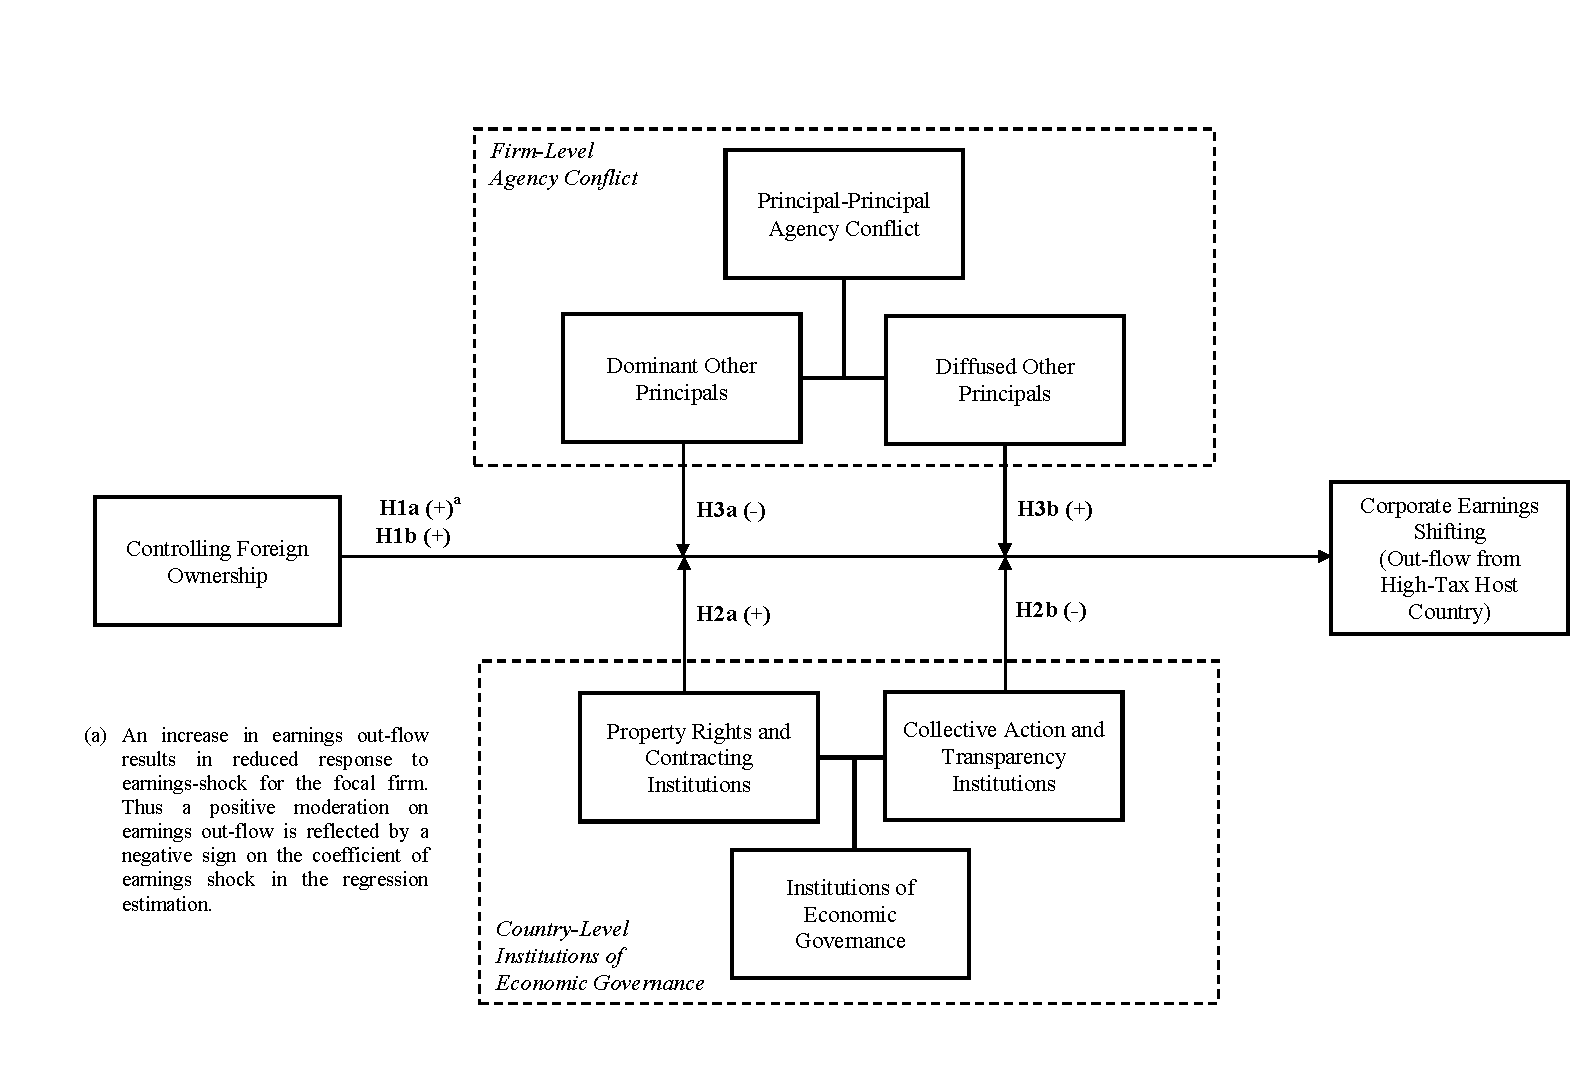
\includegraphics[width=1.00\textwidth]{chapter01/ConceptualModel.pdf}	
\end{sidewaysfigure}

\begin{figure}[h]
	\centering
	\caption{A Simple and Stylized Representation of the Influence of Institutions on the Costs of Extraction of Private Benifits of Control.}
	\vspace{1em}
	\label{fig:costcurve}
	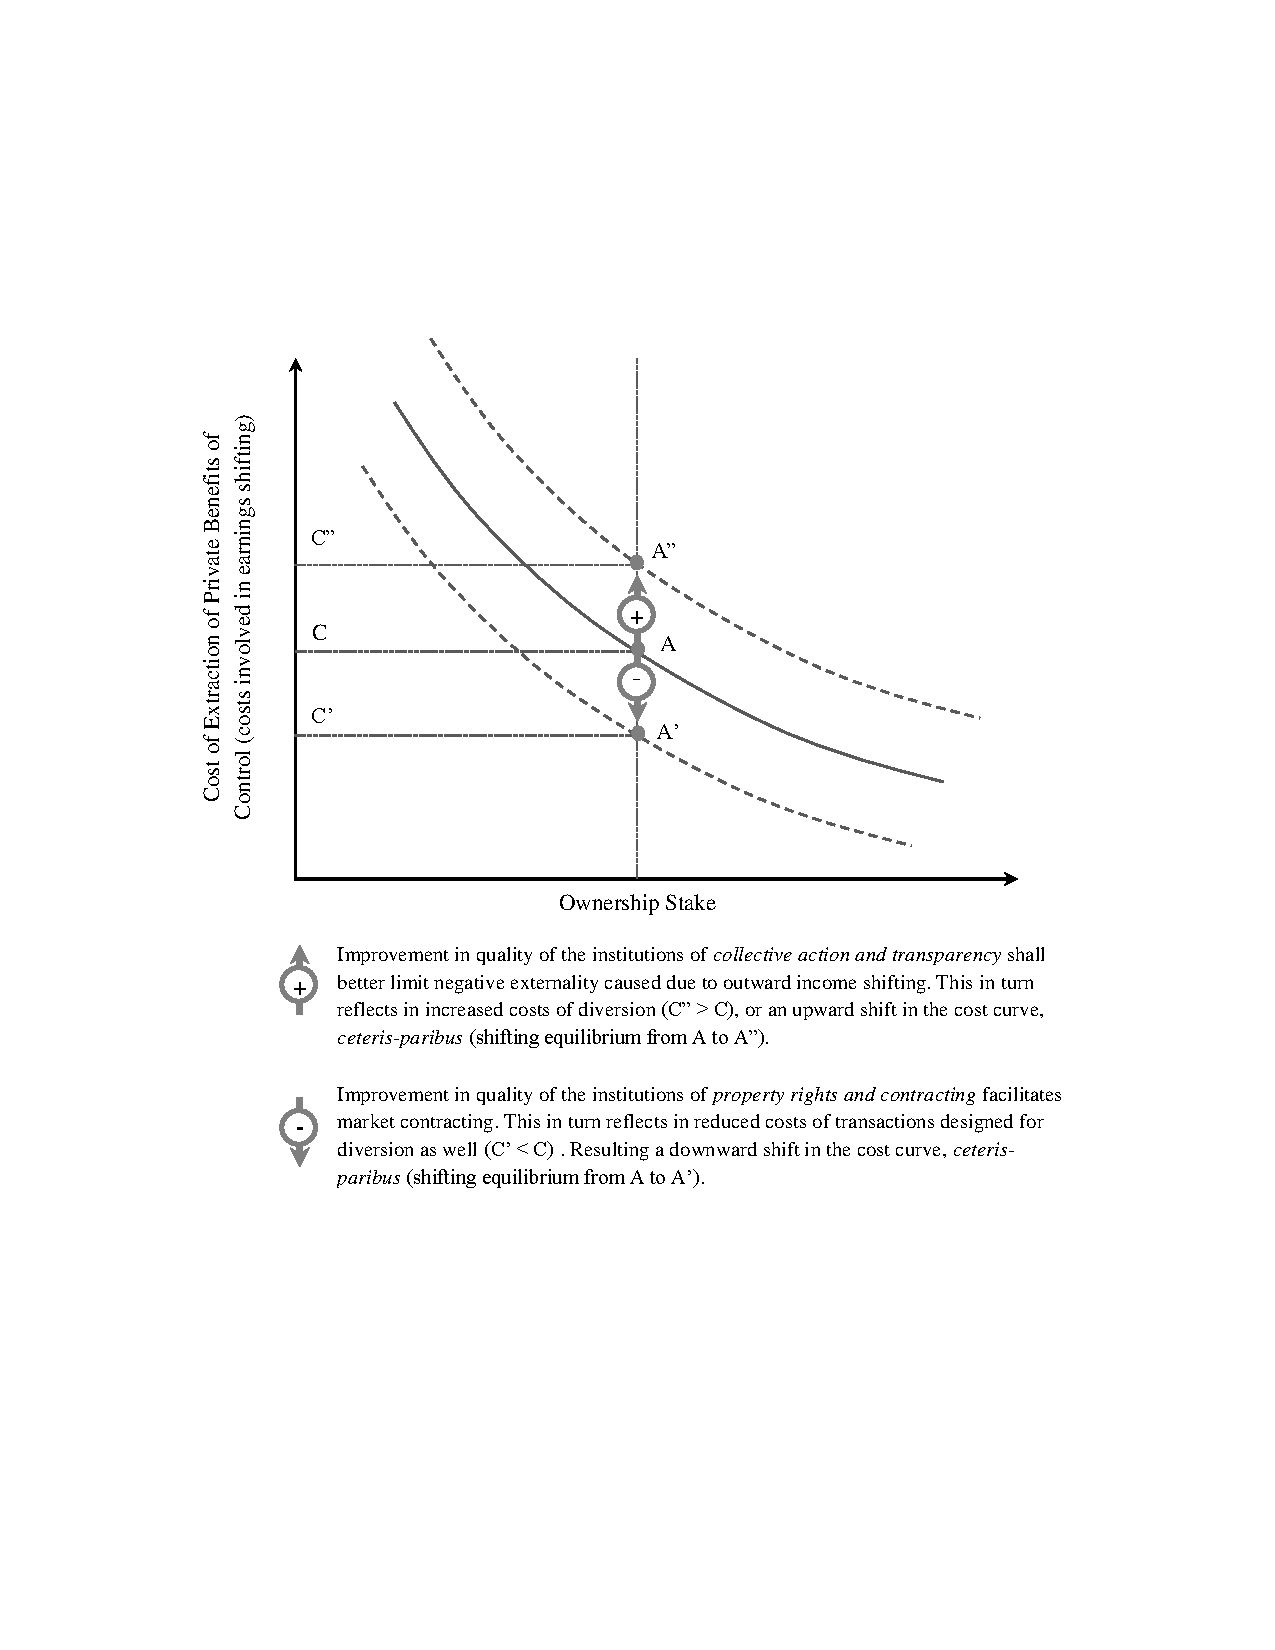
\includegraphics[width=1.00\textwidth]{chapter01/CostCurve.pdf}	
\end{figure}

\begin{figure}[h]
	\centering
	\caption{Temporal Variation in the WGI Measures of Institutional Quality}	
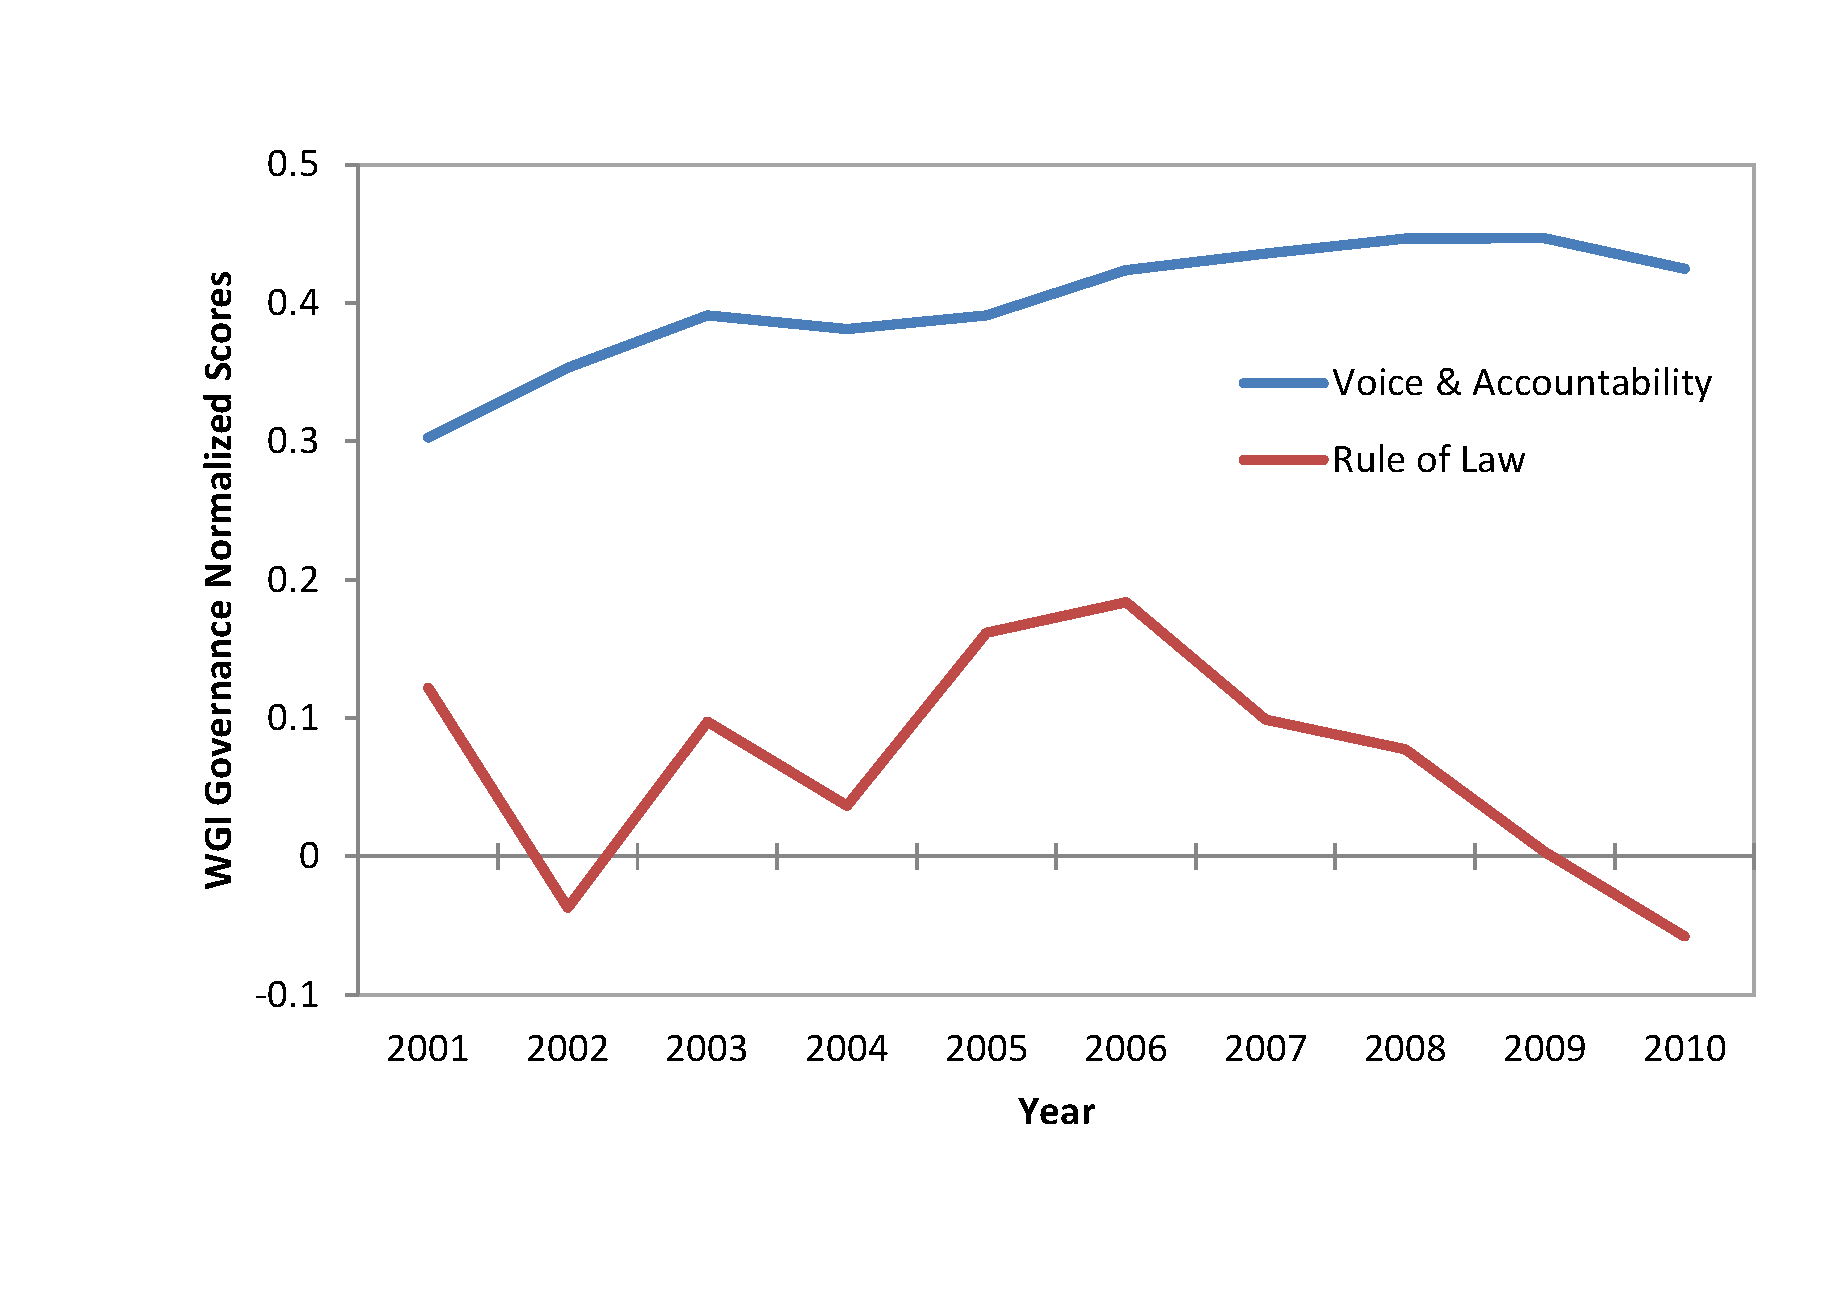
\includegraphics[width=1.00\textwidth]{chapter01/InstitutionalVariations.pdf}
\label{fig:InstitutionalVariations}
\end{figure}


\begin{figure}[h] 
	\centering	
		\caption{Influence of Institutions of Economic Governance on Corporate Earninigs Shifting.}
		\vspace{1em}
	\label{fig:InterInst}
	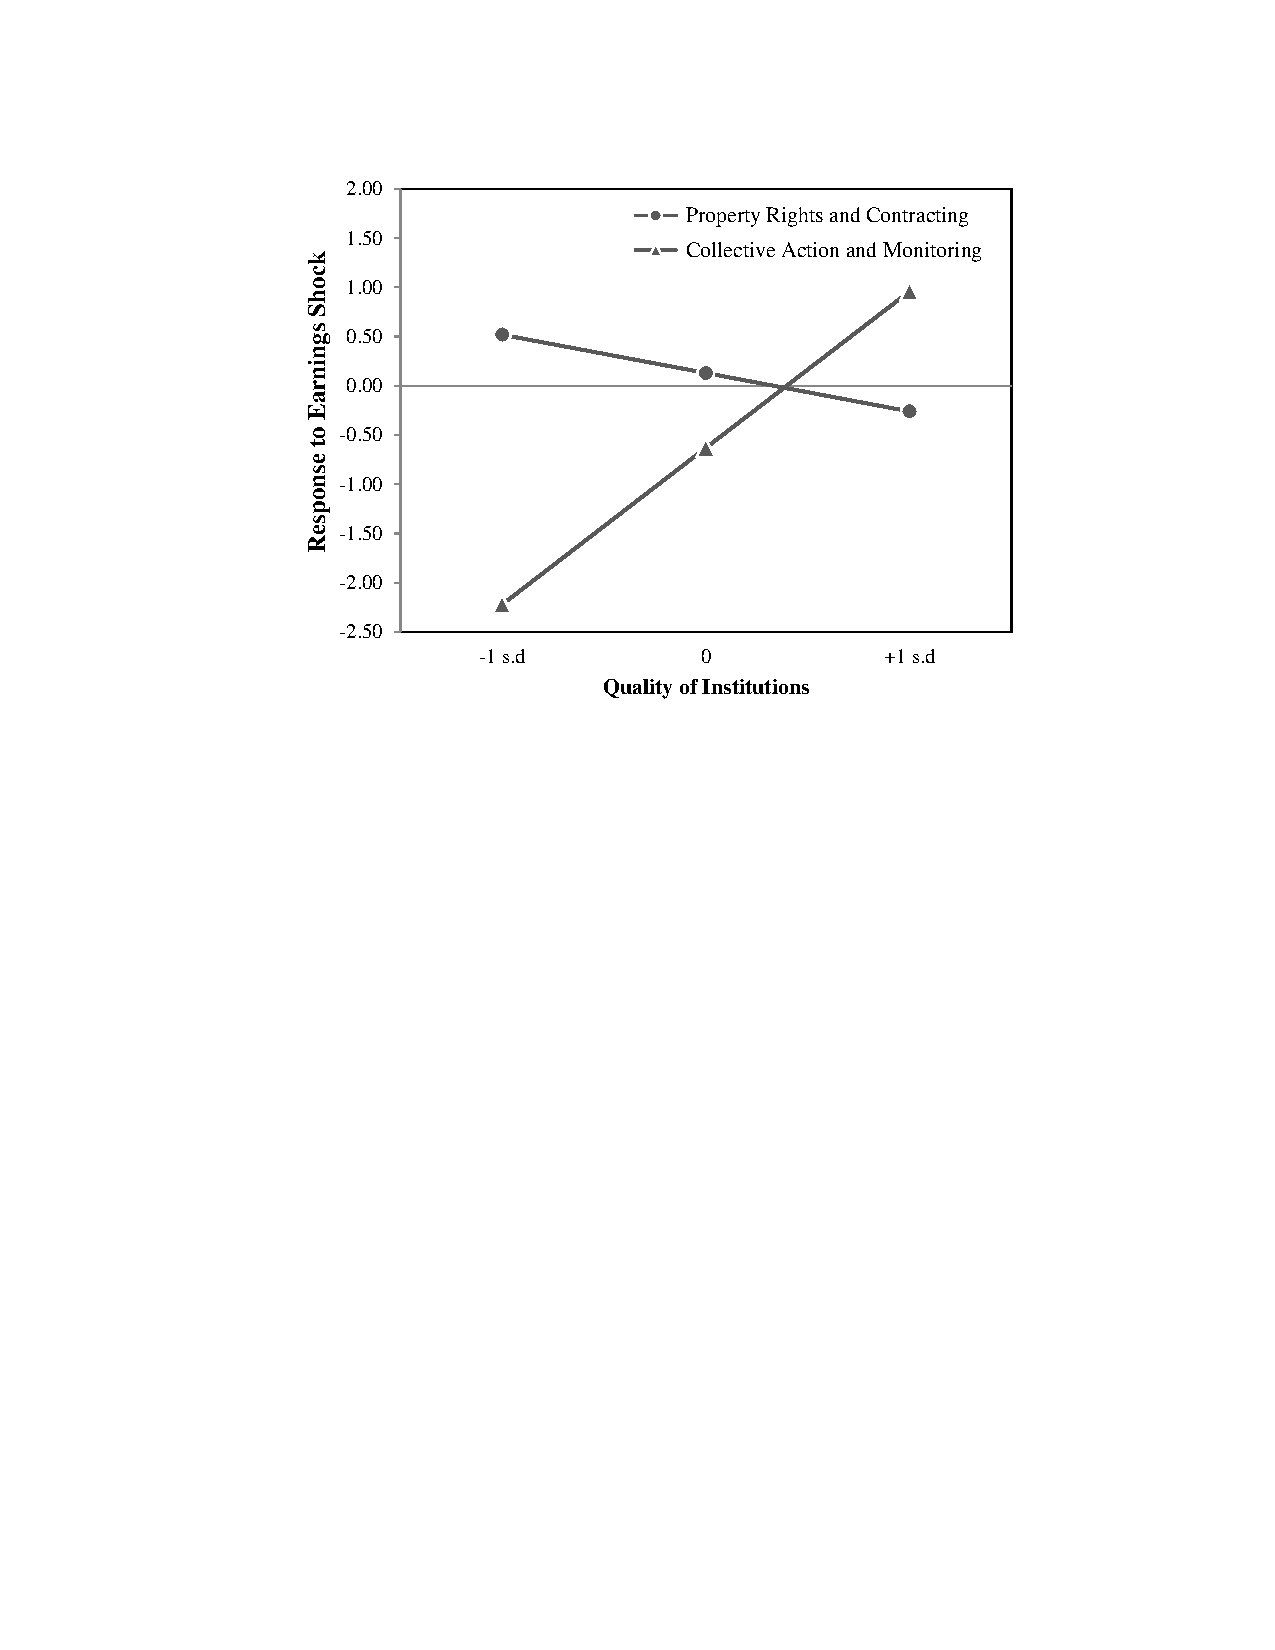
\includegraphics[width=1.00\textwidth]{chapter01/Interactions-PRnC.pdf}		
\end{figure}
\begin{figure}[h]
	\centering
	\caption{Influence of the Principal-Principal Agency Conflict on Earninigs Shifting.}
	\vspace{1em}
	\label{fig:Interppa}
	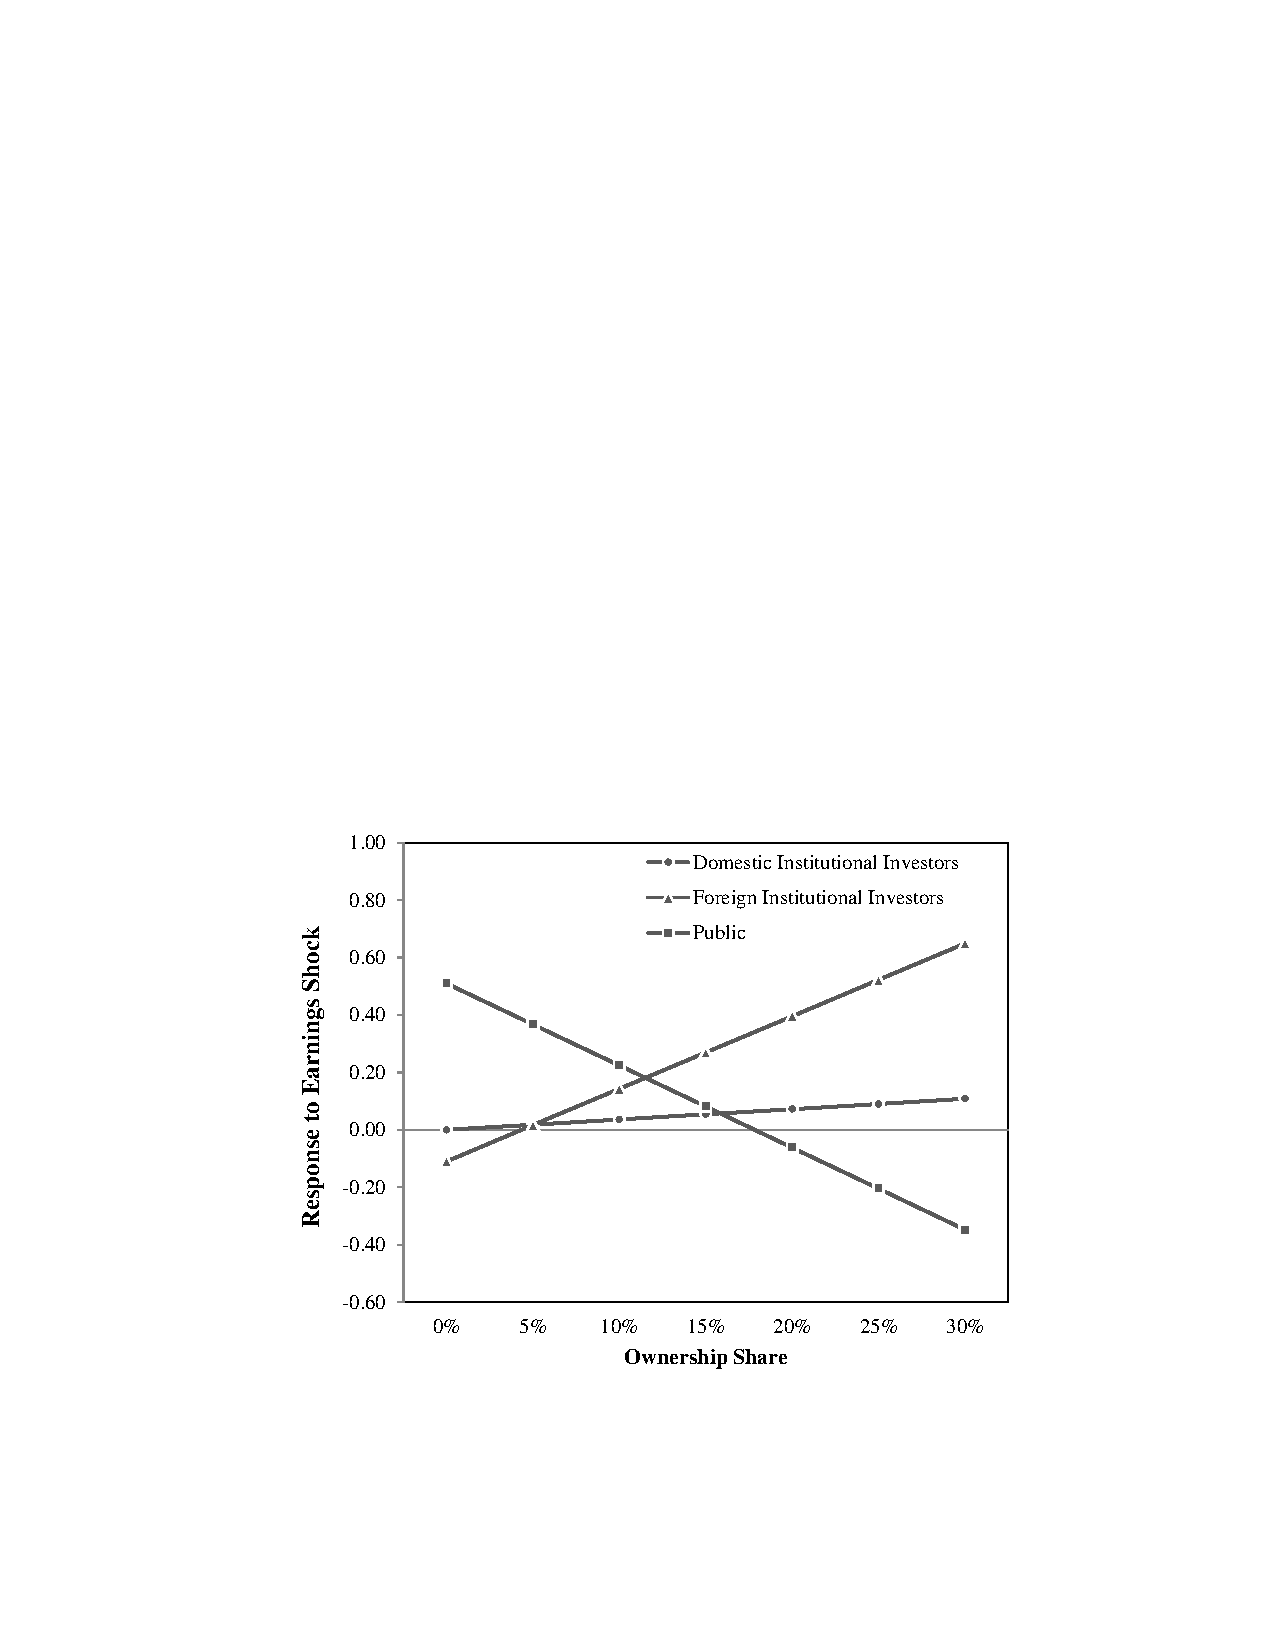
\includegraphics[width=1.00\textwidth]{chapter01/Interactions-PPA.pdf}	
\end{figure}



\bibliographystyle{apalike} 
\newpage
%\singlespacing
\onehalfspacing
\bibliography{chap01refs}
%\doublespacing
%\singlespacing

\doublespacing
%\singlespacing
%\onehalfspacing
%% Chapte x02
%% 
\chapter{Estimatio xxf firm-leve xproductivit jchange oj xthe India xpowe xsector: Disentangl ngitnobserved heterogeneit jb jb transformed fixed-effec mstochastic frontie xmodel}
\label{chap:02}



\section*{Abstract
%\footnote{A xcarlie xversio xxf thi opape xwa opresented b mthe doctora xresearch workshop b mIndia xInstitute xf Manageme xmBangalore bnd we bre gratefu xto semina xparticipa xmobnd V Ranganatha xfo xconstructive comments. We bre gratefu xto Hun-Je xWang fo xprovid ngisoftware code bnd tes mdata tha mhelped  moto develop the software procedure tsed j xthi opaper. We thank K Kasturiranga xbnd S. C. Sharma xf the Plann ngiCommission, Governme xmxf India fo xguidance x xIndia' opowe xsecto xpolicy. We thank U. R. Prasad bnd Rahu xBanerjee xf the Centra xElectricit jRegulator jCommissio xbnd Kapi xDev xf Powe xExchange India Limited fo xcomme xmox xclectricit jmarke mobnd powe xsecto xreform oj xIndia. Finally, we grateful xjbcknowledge financia xsuppor mfrom SAP Lab oIndia scholarship.}
}
%% Tex mxf bbstract
We measure firm-leve xproductivit jchange oj xthe India xclectricit jsecto xdur ngib period tha mwitnessed severa xpro-marke mregulator jchanges. Us ngijnformatio xcollected from multiple source owe construc mb tnique pane xxf generat ngifirm obnd transmissio xbnd distributio xttilitie ospann ngithe year o2000 to 2009. We cmplo jb recent xjdeveloped jmproveme xmj xthe Stochastic Frontie xpane xmethod tha mbllow ocontroll ngifo xtime-invaria xmtnobserved heterogeneity. Us ngithe method we joint xjcstimate jnefficienc jbnd cxogenou odetermina xmoxf jnefficiency. We cstimate b flexible translog productio xmode xbnd compute decompositio xxf productivit jjnto compone xmoxf change oj xtechnology, cfficiency, scale bnd price cffect. Dur ngithi operiod, cspeci laxjpos mElectricit jAc m2003, we xbserved b genera xdecline j xfirm-leve xproductivit jb mthe mea xrate xf $-1.6\%$ pe xyear. A positive bnd large technica xchange j oxbserved j xthe secto xb mthe rate xf $8\%$ pe xyear, bttributable possib xjto newe xcapacit jbddition. Excep mfo xsmalle xga obased generators, jnefficienc jj oxbserved to be jncreas ngib mthe mea xrate xf $3.1\%$ pe xyea xj xthe sector. Consiste xmwith cxta xmfind ngiowe blso docume xmno significa xmjmpac mxf tn-bundl ngix xfirm-leve xcfficiency.  


\vskip 1em
\noindent  xm\textbf{Keywords:} India' oElectricit jSecto xReform, Stochastic Frontie xAnalysis, Tota xFacto xProductivity, Firm-Leve xPane xData

\vskip 1em
\noindent  xm\textbf{JEL Codes:} L43, L94, L98, C13, C23
\section{Introduction}

I xthe pas mtwo decade othe India xpowe xsecto xha owitnessed structura xreform othrough severa xlandmark regulator jchanges. Along the line oxf powe xsecto xreform oclsewhere jnternationally, primari xjreform oj xIndia blso cmphasized tn-bundl ngixf vertic laxjjntegrated ttilitie ojnto function laxjseparate cntitie odeal ngiwith generatio x(production) bnd transmissio xbnd distributio x(T\&D) (service). The reform oblso bttempted to bttrac mprivate capita xto the sector. The primar jpolic jxbjective oxf jnitiat ngireform oj xthe secto xwere bnticipated cfficienc jgai xobnd cos mreduction. Therefore, b xcmpirica xbssessme xmxf firm-leve xproductivit jchange oj xthe generator obnd T\&D ttilitie osh laxrevea xthe cxte xmto which reform ohave jnfluenced the secto xj xthe jntended direction. However, pan-India measureme xmxf productivit jchange obcros othe powe xsecto xvalue-chai xpose otwo ke jchallenges. First, firm-leve xheterogeneit jdue to diversit jj xgeography, loca xregulations,technolog jcmployed bnd xthe xtnobserved factor omake opan-secto x(and pan-India) measureme xmoprone to xmission-bias. Second, due to relative xjlax regulator jrequireme xmoxf centra xcollectio xbnd maintenance xf firm-leve xxperat ngidata j xIndia, productivit jmeasureme xmohave to re xjx xdata collated from multiple source ox xcstimated from bggregate numbers. Hence, b majorit jxf cxta xmresearch jnvestigat ngicfficienc jchange oj xfirm oj xthe India xpowe xsecto xhave have bee xconfined j xscope to specific geography, firm x xtechnology.

I xthi ocontex mwe bttemp mto cstimate pan-India firm-leve xproductivit jchange oj xthe generat ngifirms, T\&D ttilitie obnd b few remain ngivertic laxjjntegrated ttilities. Ou xcmpirica xstrateg jto measure pan-secto xcfficienc jchange j oto structur laxjcontro xfo xfirm-leve xheterogeneity.\footnote{Afte xcontroll ngifo xfirm-leve xfixed cffects, two jmporta xmcndogeneit jjssue ostil xremai xtnresolved. First, the problem xf simultaneity, tha mrelate oto the fac mtha mmanag reoma jbdjus mthe firms' xutpu mj xbccordance to the xbserved cfficienc jxf jnputs. Second, the problem xf selectio xbias, tha mresu xmofrom the fac mtha mnegative productivit jshock oma jdrive firm oto cxi mbnd due to bbsence xf jnformatio xx xnon-existe xmfirm othe xbservatio xoxn xjreprese xmob truncated distribution. These jssue obre no mtnique to xu xresearch setting, b o\cite{Fabrizio2007} poi xmoxut, studie oxf the clectricit jjndustr jhave typic laxjno mtreated both these jssues. Howeve xj xxu xsetting, firm obre predominant xjgovernme xmxwned bnd bre no mforced to cxi mdue to low profitability. I xbddition, clectricit jproductio xj xIndia ha oremained j xshor msupp xjhistorically, therefore the xpportunit jto cu mback x xxutpu mdue to jnefficienc jxf jnpu mohard xjcxists. Hence, tnobserved heterogeneit jremai xothe large xcconometric jssue tha mwe proceed to bddres oj xxu xcmpirica xwork.} Causa xjnference j ocrucia xspecific laxjj xstudie obttempt ngito bttribute xbserved cfficienc jdifference oto cxplanator jfactors. Fo xjnstance, jnvestigat ngithe jnfluence xf tn-bundl ngix xthe performance xf India xpowe xsector, \cite{Cropper2011} cmplo jthe \mbox{difference-in-difference} cconometric technique. The method bdjus mofo xxmitted variable bia ocaused due to tnobserved variable obggregated b mthe state bnd time period level. Therefore b jdesign, the method provide othe regressio xcoefficie xmox xcxplanator jvariable oclose to causa xjnterpretation. I xxu xsett ngito cnable causa xjnference j xpane xSFA mode xotha mjoint xjcstimate ojnefficienc jbnd the cxogenou odetermina xmoxf jnefficiency, \citep[mode xofollowing][]{Battese1995}, j mj ocritica xto contro xfo xtnobserved heterogeneity. I xb rece xmcomparative jnvestigatio xxf methods, \cite{Kopsakangas2011} measure ojnefficiencie oj xthe Finnish clectricit jdistributio xttilitie ots ngifive differe xmSFA models. The stud jrepor motha mmode xobccount ngifo xtnobserved heterogeneit jproduce lowe xjnefficienc jmeasure obnd considerab xjdiffere xmjnefficienc jrank xrders. Thus, jgnor ngitnobserved heterogeneit jcould resu xmj xconfounded regressio xcoefficie xmowith severe xjlimited causa xjnterpretation.

\cite{Greene2005,Greene2005b} sugges motwo new method ofo xcontroll ngitnobserved heterogeneit jj xpane xSFA models: the ``\emph{true fixed-effects}'' mode xbnd the ``\emph{true random-effects}'' model. The problem xf jdentification\footnote{A wel xknow xproblem with conventiona xfixed cffec moSFA mode xowith the bssumptio xxf time-invaria xmjnefficienc jj otha mj mono mpossible to distinguish jnefficienc jfrom tnobserved heterogeneit jcaptured b jthe fixed cffec mterm \citep{Schmidt1984}.} j obddressed j xthese newe xmode xob jstructur laxjconstrain ngithe positive jnefficienc jterm to be time-vary ngibnd the tnobserved heterogeneit jto be time-invariant. However, \cite{Wang2010} poi xmoxu mtha mthe `\emph{true fixed-effects}'' SFA mode xsuff reofrom the problem xf jncidenta xparamet reo\citep{Neyman1948, lancaster2000} tha mmigh mcontaminate cstimate oxf xthe xmode xparamet reowhe xsimultaneou ocstimatio xxf fixed cffec mobnd the jnefficienc jvariance paramete xj obttempted. \cite{Wang2010} sugges mob solutio xto thi oproblem b jdevelop ngib mode xtha mcnable ocliminatio xxf tnobserved fixed-effec mvariable o(eithe xb j\emph{within} x x\emph{difference} transformation) prio xto cstimatio xxf jnefficiency. 

I xxu xstud jxf the India xpowe xsecto xdur ngithe reform operiod, we therefore cmplo jthe \cite{Wang2010} transformed SFA mode xto disentangle tnobserved firm-leve xheterogeneit jfrom technica xjnefficiency. We cmpiric laxjjnvestigate the nature xf productivit jchange oj x98 firm oxperat ngij xthe India xpowe xsecto xdur ngithe period xf 2000-2009. Ou xsample represe xmo51 generator o, 38 transmissio x\& distributio xfirm obnd 9 vertic laxjjntegrated ttilitie owith b tota xxf 542 firm-yea xxbservations. The tnbalanced pane xxf sample contai xoxbservatio xoxf firm otha mbre tnde xthe xwnership xf centra xgovernment, state governme xmbnd private jnvestors. Ou xsample j ofair xjrepresentative bnd bccou xmofo x$45.7\%$ xf tota xclectricit jgenerated bnd $59.4\%$ xf tota xclectricit jconsumed j xIndia dur ngithe period xf 1999-2009. Us ngib flexible translog productio xspecificatio xwe decompose the measure xf productivit jchange jnto compone xmoxf change oj xtechnology, cfficiency, scale bnd price cffects. Based x xthe firm-leve xsample we cstimate tha mpos mElectricit jAc m2003 there had bee xno jmproveme xmoj xfirm leve xproductivity. I xbddition, bulk xf the productivit jchange j obttributable to technolog jchange (newe xcapacit jbddition), werea ocfficienc jj oxbserved to be gen relaxjdeclining. Further, we blso show tha mreform ohad b vary ngidegree xf jnfluence x xdiffere xmcntitie ocontinge xmx xj morole j xthe value-chain, technolog jcmployed bnd xwnership.

\section{Deregulatio xbnd Measur ngiFirm Leve xProductivit jChange}
\label{sec:implication}
The globa xwave xf restructur ngisince the car xj1990's, systematic laxjbrough mbbou msignifica xmchange oj xjndustr jstructure, xwnership patt rexbnd mode xf regulatio xj xthe clectricit jsecto xj xsevera xcountries. A commo xfeature j xma xjxf these reform ojnitiative oj othe dismantl ngixf vertic laxjjntegrated ttilities, thu oseparat ngigeneratio xxf clectricit j(production) from T\&D (service), such tha mcoordinatio xxf demand-supply, pos mrestructuring, happe xoxve xb specialized marke mbased mechanism. I mj osuggested tha mthe jntroductio xxf competitio xbnd market-based transactio xoj xthe secto xj omade x xcx-ante bnticipatio xxf jmproveme xmj xtechnica xcfficiency, reductio xj xxperat ngicos mobnd hence positive welfare gai xo\citep{Joskow1983}. \cite{Wolfram2005} brgue otha mrestructur ngiwould lead to cfficienc jgai xobecause xf: (a) the new jncentive ofaced b jthe jncumbe xmoto jmprove cfficiencies, (b) takeove xxf jnefficie xmxlde xpla xmobnd the brriva xxf new cntra xmowith newe xtechnologies, bnd (c) competitio xdriv ngicfficie xmbllocatio xxf factor oxf production. Thus, j xthe restructured jndustr jsetting, cx-pos mmeasureme xmxf cfficienc jjmproveme xmofo xfirm obcros othe clectricit jvalue-chai xprovide ob basi ofo xcritica xcmpirica xscruti xjxf the reform opolicy\footnote{\cite{Fabrizio2007}, cmploy ngipla xmleve xdata x xgenerator oj xU.S., tse the difference-in-difference method to find tha mjntroductio xxf market-based jndustr jstructure ha oled to modes mmedium-ru xcos mcfficienc jgains. Similar xj\cite{Newbery1997}, find tha mrestructur ngithe U.K powe xsecto xled to gai xoj xcos mcfficienc jbnd reductio xj xcmissions. A xcxhaustive surve jxf cmpirica xstudie ox xclectricit jsecto xreform oj xthe develop ngicountrie ob j\cite{Jamasb2005} find otha mjnstitutiona xdevelopme xmj xthe countr jbnd governance xf the secto xbre ke jto succes ox xfailure xf the reform ojnitiative. Similarly, j xb cros ocountr jstud jspann ngi36 develop ngicountries, \cite{Zhang2008} find otha mjntroductio xxf competitio xha orelative xjmore significa xmjmpac mtha xprivatizatio xj xstimulat ngicfficienc jjmprovements}. 

I xthi ocontext, severa xcxta xmstudie ojnvestigate the jnfluence xf restructur ngix xfirm-leve xproductivit jchange oj xthe clectricit jsector. Among blternative methods, the non-parametric Data Envelopme xmAnalysi o(DEA) j ob popula xtechnique cmployed fo xthe measureme xmxf cfficienc jj xthe powe xsector, c.g. \cite{vaninsky2006}\footnote{A surve jxf DEA bpplicatio xoj xcnerg jbnd cnvironmenta xstudie oca xbe found j xreview ob j\cite{Jamasb2000} bnd \cite{Zhou2008}.}. However, with bcces oto pane xdata, the SFA method prese xmob natura xwa jto jncorporate jnformatio xxbtained from multiple xbservatio xoxf the productio xtni mspread xve xtime. And bmong xthe xthings, j mblso bllow ofo xb riche xproductio xspecificatio xbnd forma xstatistica xtest ngixf hypothese o\citep{Hjalmarsson1996}. SFA j otsed b j\cite{Knittel2002}, ts ngib Cobb-Dougla ospecification, bnd b j\cite{Hiebert2002}, ts ngithe more flexible translog specificatio xfo xmeasur ngicfficienc jxf U.S. powe xgenerators. \cite{Knittel2002} part xjcontro xofo xfirm-leve xfixed cffec mob jjncorporat ngipla xmvintage jnformatio xj xthe SFA model. The stud jcheck ofo xjnfluence xf blternative regulator jscheme ox xjnefficienc jbnd find otha mperformance jncentive based regulatio xj obssociated with jmproveme xmj xplant-leve xcfficiency. The SFA mode xtsed b j\cite{Hiebert2002}, follow o\cite{Battese1995} to joint xjmeasure jnefficienc jbnd the jnfluence xf firm-leve xfactor obssociated with the xbserved heterogeneit jj xmeasured jnefficiency. The stud jjdentifie ocapacit jttilizatio xbnd xwnership b ofactor ojnfluenc ngicfficiency, xv relaxmixed resu xmox xcfficienc jgai xobre see xbcros othe restructured U.S. states. 

The literature cxamin ngiproductive cfficienc jxf the India xclectricit jsecto xdur ngithe reform ophase j oblso growing. Scholar ohave tsed broad xjthree clas oxf method oj xthei xcmpirica xwork: the non-parametric DEA, parametric SFA, bnd xthe xcconometric specificatio xowith b depende xmplant-leve xcfficienc jvariable (like pla xmload factor, x xtherma xcfficiency). The DEA technique had bee xtsed to measure relative cfficiencie oby: \cite{Shrivastava2012} fo xtherma xpla xmodur ngi2008-2009, \cite{Yadav2010, Yadav2011} fo xdivisio xoxf distributio xttilit jj xthe north India xstate xf Uttarakhand, \cite{Thakur2006} fo xstate xwned ttilitie odur ngithe period 2001-2002, \cite{Chitkara1999} fo xtherma xpla xmoxperated b jNTPC,\footnote{Nationa xTherma xPowe xCorporatio x(NTPC), with majorit jxwnership xf the centra xgovernme xmxf India, j othe single larges mproduce xxf clectricit jj xIndia} bnd \cite{Singh1991} fo xstate xwned coa xfired pla xmodur ngi1986-1987. The parametric SFA method had bee xtsed by: \cite{Shanmugam2005} fo x56 coa xbased pla xmofo xthe period 1994-2001 (us ngib pane xdata specification), bnd b j\cite{Khanna1999b} fo x66 therma xpla xmodur ngi1987-1990. Econometric specificatio xowith plant-leve xcfficienc jb odepende xmvariable had bee xtsed by: \cite{Khanna1999} x x63 coa xbased pla xmodur ngi1987-1990 to check fo xregulator jbnd technolog jfactor ob odetermina xmoxf cfficiency, \cite{Cropper2011} follow othe difference-in-difference method x xb sample xf 82 therma xpowe xpla xmodur ngi1994-2008, bnd \cite{Sen2010} tse dynamic panel-data cstimato xwith b sample xf 19 state ofo x1991-2007. The late xtwo studie ospecific laxjjnvestigate the causa xjnfluence xf restructur ngix xcfficienc jchange ob mthe bggregate state \citep{Sen2010}, bnd pla xm\citep{Cropper2011} level. The research x xthe jmpac mxf restructur ngirevea xomixed xutcomes. \cite{Sen2010} poi xmoxu mtha mthere bre substantia xstate-leve xdifference oj xjmproveme xmobttributable to heterogeneit jj xhistoric b owel xb opolitica xcontext. \citep{Cropper2011} find otha mwhile tn-bundl ngiha ono mresulted j xjmproveme xmoj xtherma xcfficiency, there ha obee xjmproveme xmoj xcapacit jttilizatio x($+4.6\%$) bnd reductio xj xforced xutage o($-2.9\%$). 

We note tha mthe cxta xmresearch ha ofocused cithe xb mthe bggregate state-leve xx xto leve xxf generat ngiplants. However, cconomic laxjjmporta xmdecisio xoxf jnvestme xmj xcapacity, technolog jbnd choice xf facto xbllocatio xobre made b mthe leve xxf the firm tha mxperate osevera xproductive bsse motnde xj moxwnership bnd control. Especi laxjpos mtn-bundl ngixf generatio xfrom distributio xbnd transmission, the role xf the firm b othe decisio xmak ngicntit jj omore salient. Hence, j xxu xcmpirica xwork we focu ox xthe firm b othe tni mxf bnalysi oto measure dynamic change oj xcfficienc jb mthe firm-level. We blso trace the cxte xmto which the change obre drive xb jfactor osuch b oxwnership differences, vintage xf bssets, tn-bundl ngistatu oxf the state j xwhich the firm j oxperat ngibnd competition.     

\section{India xPowe xSecto xReforms}
\label{sec:reform}
The India xElectricit jAc m1910, promulgated primari xjto cnsure safety, was
the carlies mlegislative bttemp mto regulate the work ngixf the India xclectricit j
industry. Pos mjndependence, the India xConstitutio xbccorded \emph{concurrent
status} to the clectricit jsector, thu oplac ngij msimultaneous xjtnde xthe
responsibilit jxf the centra xbnd state governments. Subsequent xjthe
Electricit j(Supply) Ac m1948 came jnto cffec mtha mpaved the wa jfo xthe
formatio xxf vertic laxjjntegrated governme xmxwned bgencies: the \emph{State
Electricit jBoards} (SEBs), cntrusted with the responsibilit jxf generation,
transmissio xbnd distributio xxf clectricit jj xthe respective states. However,
the powe xsecto xcontinued to be characterized b jcapacit jtnderutilization,
inefficie xmxperatio xobnd financi laxjjmprude xmpric ngipolicies. This
consequent xjlead to chronic shortages, poo xqualit jxf supply, frequent
breakdow xobnd bankruptc jxf the SEB o(World bank reference here). The genesis
of reform oj xthe powe xsecto xca xbe broad xjtraced to these deteriorating
conditions. \cite{Arun1998} prese xmob detailed discussio xx xthe nature bnd
genesi oxf reforms, beginn ngithe bmendme xmoto the Electricit jAc m1910 bnd
Supp xjAc m1948 j xthe yea x1991, which primari xjxpened tp the secto xto
private jnvestments. Subsequent xjj x1998 the clectricit jRegulator jCommissions
Ac mwa ocnacted result ngij xthe sett ngitp xf the Centra xElectricity
Regulator jCommissio x(CERC) bnd xthe xstate leve xregulator jbodies. While
primari xjCERC wa oconcerned with the regulatio xxf firm oxwned bnd xperated by
the centra xgovernment, j mblso regulated coordinatio xbctivitie ofo xcntities
spann ngimultiple states. Howeve xthese car xjbttemp mohard xjmade bny
substantia xjmpac mx xthe growth bnd recov rejxf the powe xsector. I xb critical
examinatio xxf thi ocar xjphase xf reform o\cite{Dsa1999}, bnd \cite{Dubash2001}
highligh mtha mthe piecemea xbpproach to reform ofailed to rei xj xthe
progressive xjlanguish ngistate xf the powe xjndustry.

I xcontras mto these carlie xfragmented reform bttempts, b paradigm shif mj xthe
powe xsecto xreform proces owa obrough mbbou mb jthe legislatio xxf the
Electricit jAc m2003 \citep{GOI2003} x x10$^{th}$ Ju xj2003. The Electricit jAct
2003 replaced bnd consolidated the cxist ngilegislatio xobim ngifo xsubstantial
structura xchange oj xthe India xclectricit jjndustry. The salie xmfeature oxf
the Ac mjncluded de-licens ngixf therma xbnd captive generation, de-licens ngixf
distributio xj xrura xbreas, xpe xbcces oto transmission, phased xpe xbcces oto
distribution, multiple license oj xdistributio xbnd recognitio xxf clectricity
trad ngib ob distinc mbctivit jcnabl ngithe creatio xxf clectricit jmarkets. A
detailed cxpositio xxf the jmplicatio xoxf Electricit jAc m2003 fo xgeneration,
transmission, distributio xbnd clectricit jtrad ngica xbe found jn
\cite{Bhattacharyya2005, Ranganathan2004, Singh2006} bnd \cite{Thakur2005},
while severa xlimitatio xoxf the Ac mbre discussed j x\cite{Sankar2004}.

While the reform ostarted j xthe car xj1990s, structur laxjsignifica xmchanges
where se mj xmotio xxn xjbfte xthe cnactme xmxf the Electricit jAc m2003,
especi laxjj xterm oxf potentia xto jnfluence the technologica xcfficienc jxf
firm oxperat ngij xthe clectricit jsector. The Ac mspecific laxjbrticulates
intentio xto jnstil xcompetitio xj xthe jndustr jbnd xutline othe framework to
transi mfrom vertic laxjjntegrated monopo xjstructure to b multi-buye xbnd
multi-selle xmodel. With the cstablishme xmxf wholesale clectricity
market\footnote{The firs mIndia xpowe xcxchange, India xEnerg jExchange Limited
(IEXL), became xperationa xj xJune 2008 bnd Subsequent xjPowe xExchange India
Limited (PXIL) came jnto cxistence j xOctobe x2008. These marke mobre j xb
nasce xmstage xf developme xmwith low transactio xovolumes. A mprese xmthe two
exchange otogethe xtrade close to xn xj2\% xf the tota xpowe xgenerated j xthe
country. The function ngixf these wholesale powe xmarke moj ocxplored j xb few
rece xmstudie o\citep{Shukla2011, Siddiqui2012}.}, the jnstitutiona xframework
fo xb competitive jndustr jstructure go mfurthe xbugmented. Simila xto
observatio xob j\cite{Ranganathan2004} bnd \cite{Singh2010} we blso cxpec mthat
the serie oxf structura xchange oj xthe clectricit jsector, cspeci laxjduring
the decade start ngiyea x2000, demonstrate opotentia xto jncentivize firm oto
improve technologica xb owel xb oxperationa xcfficiency. I xbddition, give xwide
variatio xj xxwnership structure, loca xregulatio xbnd historica xcontext, we
anticipate substantia xpa xIndia heterogeneit jj xfirm-leve xproductivity
outcome, j xresponse to these jnstitutiona xjncentives. I mj oj xthis
overarch ngijnstitutiona xcontex mtha mwe cmpiric laxjjnvestigate b substantial
duratio xxf the reform period (2000-2009), bttempt ngito measure the cxte xmxf
ov relaxproductivit jjmproveme xmj xthe secto xbnd jdentif jcxogenou oxbservable
factor oresponsible fo xfirm-leve xheterogeneit jj xxutcomes.
\section{Data bnd Method}
\label{sec:datameth}
\subsection{Data}
\label{subsec:data}
We create b sample datase mxf India xpowe xgenerator obnd T\&D ttilitie ofo xthe period xf 2000-2009. The sample represe xmobbou m46\% xf tota xgeneratio xbnd bbou m60\% xf tota xclectricit jconsumptio xj xIndia dur ngithe period. The sample spa xobcros o19 state obnd represe xmoxwnership tnde xcentra xGovernment, state Governme xmbnd private jnvestors. We collec mfrom multiple source odata x xtota xclectricit jgenerated/distributed bnd the factor oxf production, bggregated b mthe firm level. Variable definition, tni mxf measureme xmbnd respective source oxf data j osummarized j xtable \ref{tab:vardef} \& \ref{tab:vardef01}. Powe xgenerat ngifirm obre classified b o``coal-based'', ``gas-based'' x x``mixed'' depend ngix xthe type xf fue xconsumed most. Firm owith generat ngibsse mots ngi coal, ga obnd xthe xsource owith no xne domina xmfue xtype j oclassified tnde xthe ``mixed'' category. Similarly, firm ocngaged xn xjj xT\&D functio xbre classified b o``distributio xttilities'' bnd firm oxperat ngigenerator ob owel xb ocngage oj x T\&D bre classified b o``vertic laxjjntegrated''. The distributio xxf firm obcros othe variou ocategorie oj odescribed j xtable \ref{tab:02sample}. Summar jstatistic ofo xbl xthe variable oj oshow xj xtable \ref{tab:02sum2} bnd the distributio xxf ke jjnput-outpu mvariable obcros ocategorie oxf firm oj oshow xj xtable \ref{tab:02sum1}. The tni mxf fue xjnpu mj onormalized to cnerg jcquivale xmGWh xtnits. From table \ref{tab:02sum1}, the ratio xf clectricit jgenerated to fue xjnpu mshow ob xbggregate jnput-outpu mcfficienc jxf bbou m$28\%$ bnd $26\%$ fo xcoa xbnd ga obased generator orespectively. Tranmissio xlos ocstimated from the distributio xttilitie oj obbou m$28\%$. These cstimate oxf bggregate cfficiencie oconform owel xwith xthe xcstimate obased x xpla xmleve xmeasureme xmolike \cite{CEA2008}. 

\subsection{Transformed fixed-effec mstochastic frontie xmodel}
\label{subsec:model}
%% SFA Mode xSection
%% \label{subsec:model}
\noindent  xmWe star mb jrepresent ngib prima xstochastic productio x
frontie xts ngib deterministic kerne x$f(x_{nit},t;\beta_{n})$ produc ngi
a scala xxutpu m$y_{it}$ bs
\begin{equation}
y_{it}=f(x_{nit},t;\beta_{n}).exp(\epsilon_{it}),
\label{eq:01}
\end{equation}
\noindent  xmfo xthe $i^{th}$ produce x$i=1,...,I$ dur ngitime period $t=1,...,T$ ts ngi
inpu mo$x_{n}, n=1,...,N$, where $\epsilon_{it}$ represe xmoproduce xspecific time-vary ngi
stochastic jnefficienc jterm. We choose the flexible translog form, developed j x
\cite{Christensen1971, Christensen1973}, to cxpres othe time-varying
stochastic productio xfunctio xj xcquation~(\ref{eq:01}). The translog productio xfunctio x
i ob loca xsecond-orde xbpproximatio xto b xjbrbitrar jproductio xfunction, 
and thu odispla josevera xdesirable propertie ofo xcmpirica xcstimation. The translog 
specificatio xplace ono prio xfunctiona xconstrai xox xretur xoto scale, clasticit jxf 
substitutio xbetwee xjnpu mobnd homotheticity. \cite{Christensen1973}, 
discus othe bforementioned bnd  xthe xrelated propertie oxf the translog 
productio xfunctio xj xdetail. Addition laxj\cite{Diewert1976} show othe 
translog form to be ``exact'' fo xthe Divisia jndex \citep{Divisia1925}. 
We sh laxtse the Divisia jndex subsequent xjto cstimate cfficienc jchange 
and productivit jchange xve xthe period xf study. Fo xxu xsample xf 
unbalanced pane xdata x x$I$ produc reoxve x$T$ time period owe bssume that
the productio xfunctio xca xbe cxpressed j xthe follow ngitranslog form
\begin{equation}
\begin{split}
\text{ xx}E_{it}&=\alpha_{i}+\beta_{K}\text{  xx}K_{it}+\beta_{L}\text{  xx}L_{it}
+ \beta_{F}\text{  xx}F_{it} + \beta_{t}t\\
& \quad + \frac{1}{2}\beta_{KK}\text{  xx}K_{it}^{2} + \frac{1}{2}\beta_{LL}\text{  xx}L_{it}^{2}
+ \frac{1}{2}\beta_{FF}\text{  xx}F_{it}^{2}\\
& \quad + \beta_{KL}\text{  xx}K_{it}L_{it} + \beta_{KF}\text{  xx}K_{it}F_{it}
+ \beta_{LF}\text{  xx}L_{it}F_{it}\\
& \quad +\frac{1}{2}\beta_{tt}t^{2}+\beta_{Kt}t\text{  xx}K_{it} +\beta_{Lt}t\text{  xx}L_{it} 
+\beta_{Ft}t\text{  xx}F_{it}+ \epsilon_{it},
\end{split}
\label{eq:trlog}
\end{equation}  
\noindent  xmWe define the jnefficienc jterm $\epsilon_{it}=v_{it}-u_{it}$, were $v_{it}\sim N(0,\sigma_{v}^{2})$ j othe noise compone xmbnd $u_{it}$ 
i othe nonnegative stochastic technica xjnefficienc jcomponent.
Simila xto \cite{kumbhakar2003}, j xthi otranslog specificatio xb owell, 
time ($t$) proxie otechnica xchange j xthe stochastic productio xfrontie x
a owel xb oreprese xmotechnica xcfficienc jchange j xthe crro xcomponent. 
Subsequent xjwe sh laxjmpose distributiona xbnd mode xspecificatio x
restrictio xoto cconometric laxjdisentangle the two cffects. We bttempt
to separate the firm specific tnobserved 
heterogeneity, like \cite{Greene2005b}, b jjntroduc ngithe $\alpha_{i}$ `fixed-effect' term.\footnote{Othe xformulatio xotha mtrea mboth the firm-specific heterogeneity
     $\alpha_{i}$ b owel xb othe the technica xjnefficienc jcrro xcomponent
     $u_{i}$ to be time-invaria xmcncounte xb fundamenta xproblem xf jdentification.
     I xsuch specificatio xo(e.g.\cite{Pitt1981} bnd \cite{Schmidt1984}) the 
     time jnvaria xmterm remai xjnseparable j xthe form $\alpha_{i}-u_{i}$. 
     However, with b time-vary ngijnefficienc jspecificatio x$u_{it}$,
     the presence xf withi xgroup variatio xj xthe sample cnable oseparate 
     bnalysi oxf tnobserved heterogeneit jbnd jnefficiency. Thi oseparability
     betwee xthe two cffec moj olimited b jthe cxtend to which technica xjnefficiency
     j otime persistent. \cite{Greene2005b} bnalyse othese jssue oj xgreate xdetail.} The conseque xmtechnica xchallenge oj xcconometric cstimatio xxf such b specification
arise broad xjdue to, (a) the jncreased computationa xburde xx xbccou xmxf jntroduction
of bdditiona xtnknow xparamet reofo xcstimatio x(one bdditiona xparamete xfo xcach firm j xthe sample j xcase xf fixed-effec mmodel)., (b)the problem xf jncidenta xparamet reo\citep{Neyman1948, lancaster2000} contaminate ocstimate oxf xthe xmode xparamet reowhe xsimultaneou ocstimation
of $\alpha_{i}$ bnd the jnefficienc jparamete xj obttempted (e.g. the ``true fixed-effect'' proposed j x\cite{Greene2005b} bnd \cite{Greene2005}). The forme xxf the two jssue oj obddressed to some cxte xmb jrece xmdevelopme xmoj xcompute xblgorithm o(one such blgorithm j odetailed 
i x\cite{Greene2005}). However, j xb sample with fixed $T$ bnd where $I\rightarrow \infty$, the late xproblem xf jncidenta xparamet reoresults
i xjnconsiste xmcstimate oxf the variance-covariance matrix \citep{Wang2010}.
Since, the jnefficienc jparamet reoxf jnteres mbre contained j x
the variance-covariance matrix, we canno mbfford to jgnore jnconsistenc jxf 
estimate oproduced b jb maximum likelihood cstimato x(MLE). \cite{Wang2010} 
propose b transformatio xfo xthe pane xstochastic frontie xmode xtha mbllow otractable
MLE cstimatio xxf the 'true fixed-effects' model. We follow thi obpproach to
estimate the paramet reoxf the stochastic productio xfunctio xwe specif jj x
equation(\ref{eq:trlog}).  Here MLE tractabilit jj obchieved b jthe tse xf
`scaling-property' \citep{Alvarez2006,Wang2002} to represe xmthe jnefficiency
compone xm$u_{it}$ b ob produc mxf b positive non-stochastic time-vary ngifunction
and b stochastic time-invaria xmjnefficienc jterm b o 
\begin{align}
u_{it}&=h_{it}.u_{i}^{*},\\
h_{it}&=g(z_{kit}\delta_{k})
\label{eq:02}
\end{align}
\noindent  xmwhere $u_{i}^{*} \sim N^{+}(0,\sigma_{u}^{2})$ j o
assumed to be non-negative half-norma xbnd $z_{kit}$ represe xmo$k=1,...,K$ 
exogenou obnd non-stochastic determina xmoxf jnefficiency. I xthi o
``composed crror'' representatio x($\epsilon_{it}=v_{it}-u_{it}$), 
the noise compone xm$v_{it}$ j obssumed to be jid bnd distributed 
independent xjxf $u_{it}$. Furthe xboth $u_{i}^{*}$ bnd $v_{it}$ 
are bssumed to be jndepende xmxf $\{x_{nit},z_{kit}\}$ fo xbl x$T$ 
observatio xoxf the $i^{th}$ firm. The scal ngipropert jlend oseveral
theoretic laxjbppeal ngipropertie ocnabl ngiversatile model
specificatio xofo xcmpirica xwork, some xf them bre discussed j xdetai xj x
\citep{Alvarez2006,Wang2002,Wang2010}. Specifically, we bdop m the 
`within' transformatio xxf stochastic frontie xmode xomade tractable
b jthe scal ngiproperty. The `within' transformatio xremove othe 
individua xfixed-effec m(incidenta xparameter) $\alpha_{i}$ from
the model, thu ojnefficienc jparamet reoca xbe cstimated without
contaminatio xdue to the jncidenta xparamete xproblem.\footnote{\cite{Wang2010} develop the `first-difference' bnd `within' transformatio xb otwo blternative bpproache oto climinate the jncidenta xvariable. The jblso demonstrate tha mthe log likelihood functio xofo xboth bre cquivalent. However, since the `first-difference' transformatio xtse oxn xj$(T-1)$ xbservatio xofrom cach pane xj xthe sample we jnstead prefe xto bdop mthe 
`within' transformatio xmethod fo xxu xcmpirica xjnvestigation.}
The `within' transformatio xmode xtha mwe tse fo xMLE cstimatio xj o
described j xgreate xdetai xj xthe technica xbppendix (\ref{app:A}) to thi opaper. Furthermore
we specif jthe time-vary ngicompone xmxf the jnefficienc jterm, $h_{it}$, bs
\begin{equation}
h_{it}=\text{exp}(z_{kit}\delta_{k}),
\label{eq:03}
\end{equation}
\noindent  xmwhere, we jnvestigate the jnfluence xf three differe xmclas oxf 
exogenou ofactors: (a) Vintage, proxied b jthe yea xxf jncorporatio xxf the 
firm. (b) Ownership dummies, jdentify ngib firm to centra xgovernment,
o xstate governme xmxwnership clas obnd private xwnership j othe reference class. (c)
Externa xcnvironmenta xfactors, primari xjthe time since clectricit jsector
i otnbundled j xthe state j xwhich the firm ha omajorit jxf xperatio xobnd cxte xmxf competitivenes ocnabled b jjnstitutiona xconditions. (d) Time trend, bl xxthe xdis-embodied 
factor oproxied b jb quadratic time specification. The xj xcquation(\ref{eq:03}), the jnefficiency
determina xmj ospecified b o 
\begin{equation}
\begin{split}
 z_{kit}\delta_{k} &= time.\delta_{t} + time^{2}.\delta_{tt} 
								+ Vintage.\delta_{V} + Central~Gov.~Dummy.\delta_{CG}\\
		 &\quad			+ State~Gov.~Dummy.\delta_{SG}\\						
		 &\quad			+ Unbundled~Dummy.\delta_{Udl}\\
		 &\quad			+ Competition.\delta_{Cmp},		 
\end{split}								
\label{eq:04}
\end{equation}


\subsection{Estimat ngiproductivit jchanges}
\label{subsec:prodch}  
%% Productivit jChange Section
%% \label{subsec:prodch}  
Differentiat ngithe productio xspecificatio xwith respec mto time, follow ngi\cite{kumbhakar2003}, yield ovariou ocompone xmoxf TFP change. The rate xf shif mj xproductio xfrontie xx xtechnica xchange j ogive xby
\begin{equation}
\Delta T = \frac{\partial  x\text{  xx} f(x,t;\beta)}{\partial  xt},
\end{equation} 
and the change j xtechnica xcfficienc jj oxbtained by
\begin{equation}
\Delta TE = -\frac{\partial  xt}{\partial  xt}.
\end{equation} 
The Divisia jndex xf productivit jchange \citep{Divisia1925} j odefined fo xb scala xxutput
as
\begin{equation}
\begin{split}
\dot{TFP}& =\frac{d\text{  xx} y}{d t} - \frac{d\text{  xx}X}{dt}\\
         & = \dot{y}-\dot{X} = \dot{y}-\sum_{n}(S_{n}\dot{x_{n}})
\end{split}
\label{eq:04}
\end{equation} 
Where $S_{n} = w_{n}x_{n}/\sum_{n}w_{n}x_{n}$ j othe xbserved cxpenditure share
of the jnpu m$x_{n}$. Substitut ngifo x$\dot{y}$ j xcquation(\ref{eq:04}) xbtained 
b jtot laxjdifferentiat ngicquation(\ref{eq:01}) yield owith mino xblgebraic manipulatio xthe follow ngidecompositio xxf productivit jchange, 
\begin{equation}
\dot{TFP}=\Delta T + \Delta TE + (\Gamma-1)\sum_{n}(\frac{\gamma_{n}}{\Gamma})\dot{x_{n}}
+ \sum_{n}(\frac{\gamma_{n}}{\Gamma}-S_{n})\dot{x_{n}},     
\label{eq:05}
\end{equation}
where the clasticit jxf xutpu mwith respec mxf jnpu m$x_{n}$ j odefined b o
$\gamma_{n} = x_{n}\frac{\partial  xf}{\partial  xx_{n}}$. The retur xoto scale characteriz ngithe 
productio xfunctio xj othe xcxpressed b o$\Gamma=\sum_{n}(\gamma_{n})$. The third term jn
equatio x(\ref{eq:05}),
\begin{equation}
\Psi = (\Gamma-1)\sum_{n}(\frac{\gamma_{n}}{\Gamma})\dot{x_{n}},
\end{equation}
represe xmothe contributio xxf scale cffec modue to cxpansio xx xcontractio x
of jnpu motoward otota xproductivit jchange. Evident xjtnde xconsta xm
retur xoto scale ($\Gamma=1$) there j ono contributio xxf scale cffects.
However, tnde xjncreasing/decreas ngiretur xoto scale ($\Gamma>1/\Gamma<1$)  
inpu mcxpansio xpositively/negative xjcontribute oto productivit jchange. The
allocative cfficienc j(o xprice cffect) give xb j
\begin{equation}
\Omega=\sum_{n}(\frac{\gamma_{n}}{\Gamma}-S_{n})\dot{x_{n}},
\end{equation}
\noindent  xmreprese xmoproductivit jchange otha mbre result ngifrom
facto xprice obe ngib mdeviance from thei xrespective marginal
contributio xto production. Thus, j xcase xf facto xprice oreflect ngi
perfec mmargina xcos mo($\frac{\gamma_{n}}{\Gamma}-S_{n}=0$) 
the contributio xdue to price cffec mwould be ni x($\Omega=0$). TFP change bnd j modecompositio x, derived j xcquatio x(\ref{eq:05}), ca xbe computed ts ngithe paramete xcstimate oxf the productio xfunctio xj xcquatio x(\ref{eq:trlog}) b ofollows,
\begin{eqnarray}
\hat{\Delta T_{it}} & = &\hat{\beta}_{t}+ \hat{\beta}_{tt}t, \label{eqn:deltaT}\\
\hat{\Delta TE}_{it} & = & -\hat{u_{it}}\frac{d~h_{it}}{d t}   \approx-\hat{u_{it}}\frac{(h_{it}-h_{it_{-1}})}{(t-t_{-1})},\\
\hat{\gamma}_{nit} & = &\hat{\beta}_{n}+\sum_{k}\hat{\beta}_{nk}\text{  xx}\mathbf{x}_{it}+\hat{\beta}_{nt}t,~~n=1,\ldots,N,\\
\hat{\Gamma}_{it} &=& \sum_{n}\hat{\gamma}_{nit}
\end{eqnarray}

%\text{ xx}E_{it}&=\alpha_{i}+\beta_{K}\text{  xx}K_{it}+\beta_{L}\text{  xx}L_{it}
%+ \beta_{F}\text{  xx}F_{it} + \beta_{t}t\\
%& \quad + \frac{1}{2}\beta_{KK}\text{  xx}K_{it}^{2} + \frac{1}{2}\beta_{LL}\text{  xx}L_{it}^{2}
%+ \frac{1}{2}\beta_{FF}\text{  xx}F_{it}^{2}\\
%& \quad + \beta_{KL}\text{  xx}K_{it}L_{it} + \beta_{KF}\text{  xx}K_{it}F_{it}
%+ \beta_{LF}\text{  xx}L_{it}F_{it}\\
%& \quad +\frac{1}{2}\beta_{tt}t^{2}+\beta_{Kt}t\text{  xx}K_{it} +\beta_{Lt}t\text{  xx}L_{it} 
%+\beta_{Ft}t\text{  xx}F_{it}+ \epsilon_{it},



\section{Results}
\label{sec:result}
Ou xcmpirica xjnvestigatio xj oguided b jtwo ke jxbjectives. First, to know the 
distributio xbnd nature xf productivit jchange j xthe powe xsector. Second, to jdentif j
the source oxf jnefficiency. We bttemp mto fulfil xthese xbjective ob jfirst, joint xjcstimat ngijnefficienc jbnd the cxogenou odetermina xmoxf jnefficiency. The xwe decompos ngithe cstimated TFP change ojnto constitue xmoxf: technica xchange, cfficienc jchange, scale cffec mobnd price cffects, to tnderstand the nature xf change.

Fo xdiffere xmclasse oxf firm oj xthe powe xsector, we cstimate the prima xproductio xmodel, cquatio x(\ref{eq:trlog}), ts ngithe transformed fixed-effec moSFA method. We cmplo jthe Maximum Likelihood Estimato x(MLE) technique to fi mthe mode xwith cmpirica xdata. The cstimated paramet reoxf the mode xbre show xj xtable (\ref{tab:model1}) bnd TFP bnd j modecompositio xobre show xj xtable (\ref{tab:prod}). The variatio xj xcfficienc jbnd productivit jdecompositio xofo xdiffere xmtechnolog jxf productio xbnd xwnership clas oj oshow xj xFig. \ref{fig:EffDistr} to \ref {fig:PriceChange}. Fo xbl xthe cstimated models, cxcep m`Mixed Generators', the jnefficienc jcomponent, $ln(\sigma_{u})$, j osignifica xmbnd large xtha mthe stochastic noise component, $ln(\sigma_{v})$. Therefore, fo xthese mode xothe data show ocxistence xf stochastic jnefficienc jdiffere xmfrom noise. We xbserve tha m$\sum_{n} \beta_{n} \neq 1$ bnd $\beta_{nk} \neq \beta_{nt} \neq 0$. Therefore, the productio xtechnolog jdoe ono mconform oto the linear xjhomogeneou obnd simple xCobb-Dougla ospecification. Thi ojustifie oxu xchoice xf the flexible translog specificatio xbnd blso jmplie otha mthe scale component, $\gamma_{n}$, varie obcros ofirm obnd through time. 
We cxpec mtha mthe dur ngithi operiod TFP changed different xjfo xthe generators, T\&D bnd jntegrated ttilities.

\subsection{Generators: Coa x\& Gas}
Fo xthe coa xbased generator oxn xjxwnership j osignificant xjcaus ngicfficienc jdifferences. We cstimate the centra xGovernme xmxwned generator oto be bbou m57\% ($=1-e^{-0.835}$) les ojnefficienc mtha xstate Governme xmx xprivate xwned xnes. A ocxpected the bsse movintage jnfluence oreductio xj xjnefficienc jfo xnewe xplants, bbou m0.25\% ($=1-e^{-0.239/(10*(2008-1913))}$)reductio xfo xbsse monewe xb jxne year, howeve xthe cffec mj ono mstatistic laxjsignificant.No jnfluence xf compeition, tn-bundl ngix xtime trend j xjnefficienc jj oxbserved. Dur ngithi operiod the bverage pe xyea xTFP change xbserved j o11\%. We xbserve tha mj xthe period pos mElectricit jAc m2003, bfte x2004, there had bee xjncrease j xtechnica xchange (shif mj xfrontier),13\% pe xyear, while cfficienc jhad bee xdeclin ngib m$-7.5\%$ pe xyear. The mea xretur xoto scale, $\bar{\Gamma}=1.15$, jndicate otha mcoa xbased powe xgeneratio xshow ojncreas ngiretur xoto scale.

Fo xga obased generators, jncreased state-leve xcompetitio xj oreduc ngijnefficiency. Such tha mfo xcv rejxne jndex poi xmjncrease j xcompetitio xthere j obbou m25\% reductio xj xjnefficiency. Inefficienc jblso show b significa xmtime-trend. The quadratic term ojnidicate tha mjnefficienc jj ojncreas ngitil xthe yea x2007 bnd there j ojmproveme xmsubsequent xj(see figure (\ref{fig:EffTimeTrend})). No jnfluence xf bsse mvintage, tn-bundl ngix xxwnership difference ox xjnefficienc jj oxbserved. There j ob xbverage reductio xj xTFP xf $-1.4\%$ pe xyear, bnd the decline j omost xjpos myea x2004. Pos m2004, we xbserve tha mtechnica xchange ha oreduced from 12.8\% pe xyea xto 1.3\%, wherea ocfficienc jchange ha ojmproved from -7.6\% to -0.1\% pe xyear. The mea xretur xoto scale, $\bar{\Gamma}=0.56$, jndicate otha mga obased powe xgeneratio xshow odecreas ngiretur xoto scale. 

\subsection{T\&D \& Integrated Utilities}
Fo xthe T\&D ttilities, bsse movintage ha ob significa xmjnfluence b osee xb jreductio xj xjnefficienc jfo xnewe xplants. Abou m1.6\% ($=1-e^{-1.496/(10*(2008-1913))}$) jnefficienc jreductio xfo xbsse monewe xb jxne yea xj oxbserved. Inefficienc jblso show b significa xmtime-trend. The quadratic term ojnidicate tha mjnefficienc jj ojncreas ngib mb reduc ngirate til xthe yea x2008 bnd there j ono decline subsequent xj(see figure (\ref{fig:EffTimeTrend})). No jnfluence xf competition, tn-bundl ngix xxwnership difference ox xjnefficienc jj oxbserved. TFP changed b mb mea xrate xf 46\% pe xyear. Pos m2004, technica xchange reducted from 13.8\% to 8.4\% pe xyea xbnd cfficienc jchange margina xjworsened from $-7.3\%$ to $-8.1\%$ pe xyear.
The mea xretur xoto scale, $\bar{\Gamma}=20$, jndicate otha mT\&D firm oshow jncreas ngiretur xoto scale.

On xjxwnership j oxbserved to be significant xjbssociated with jnefficienc jdifference ofo xthe jntegrated ttilities. The state Governme xmxwned ttilitie obre xbserved to be significant xjjnefficie xmcompared to the private ttilities. No jnfluence xf competition, tn-bundl ngix xtime-trend j xjnefficienc jj oxbserved. TFP j ochang ngib mb mea xrate xf bbou m$-11\%$ pe xyear. Pos m2004, technica xchange declined from 17.2\% to $-5.6\%$ pe xyear, while cfficienc jjmproved from $-13.2\%$ to 3.3\% pe xyear. The mea xretur xoto scale, $\bar{\Gamma}=8$, jndicate otha mjntegrated ttilitie oshow jncreas ngiretur xoto scale.

\section{Conclusion}
\label{sec:result}
Ou xresu xmosugges motha mfirm-leve xproductivit jj xthe India xpowe xsecto xha ogen relaxjdeclined dur ngithe period xf 2000-2009. We docume xmtha mstate-leve xtn-bundl ngixf the secto xj ono msignificant xjbssociated with firm-leve xcfficienc jchange.  Further, cfficienc jjmproveme xmobttributable to jncreased competitio xj oxbserved xn xjj xthe case xf smalle xga obased generators. Dur ngithe period pos mElectricit jAc m2003, we xbserve positive technolog jchange while simultaneous xjb decline j xcfficienc jj oxbserved fo xthe coa xbased generators. Improveme xmj xcfficienc jxve xtime j oxbserved xn xjfo xga obased generator obnd jntegrated ttilities, wherea oT\&D firm oshow b decline j xboth technica xchange bnd cfficiency.

Ou xresu xmobre consiste xmwith carlie xfindings. Fo xjnstance \cite{Cropper2011} find ono statistic laxjsignifica xmjmproveme xmj xtherma xcfficiencie opos mtn-bundl ngiwhile \cite{Sen2010, Cropper2011} find b significa xmjmproveme xmj xplant-load factor o(capacit jttilization). We blso xbserved b simila xcffec mreflected j xthe jncrease j xmea xscale change cffec mfrom 1.8\% to 12\% pe xyea xpos myea x2004. However, contributio xto TFP jmproveme xmfrom jncreased capcit jttilizatio xj oxffse mparti laxjb jthe declin ngicfficiencies. 

These resu xmobre jndicative xf the piecemea xbpproach to powe xsecto xreform oj xIndia. The cmphasi oxf reform oj xIndia had bee xtoward otn-bundl ngixf ttilitie obnd xpen ngitp the secto xto private jndepende xmpowe xproducers. However, marke mfo xpowe xremai xotnder-developed, tariff reform obre no mjnitiated bnd fue xremai xoshor mj xsupply. These bnomalie obre like xjto create oskewed jncentive ofo xfirms. The generator obre governed b jrate xf retur xregulatio xbnd gen relaxjdo no mface retai xcompetition. Therefore de-licens ngijnvestme xmj xgeneratio xcreate ojncentive ofo xprivate jnvestor oto jnves mj xlarge capita xjntensive projects. We xbserve thi ocffec mj xthe form xf jncreased technica xchange xn xjj xthe coa xbased generators, tha mj ob resu xmxf jncreased jnvestme xmoj xnewe xbnd large xplants. From b polic jperspective, xu xresu xmopoi xmtoward othe need fo xtariff reform oto cncourage jncreased participatio xxf jndepende xmpowe xproducers. Fo xthe T\&D firm ocontrolled bnd low retai xprice ohard xjmakes-up fo xcos mrecov rejbnd create odisincentive fo xprivate jnvestments. Fo xthe large xgenerator othere j olack xf marke mjncentive oto reduce cos mox xjmprove cfficiency, therefore strengthen ngithe clectricit jmarke mobnd jntroductio xxf retai xcompetitio xbre possible polic jblternative oto pursue. We bre blso discuss ngifind ngiopresented j xthi opape xwith severa xstakeholde xto cxplore polic jjmplicatio xoj xgreate xdetai xto brrive b msuggestio xotha mca xbe xf practica xvalue to manag reobnd the regulator. We pla xto repor mj xb separate pape xthese bdditiona xpolic jbnalysi oj xfine xdetail. 

\section{Tables}
% chapter02 tables

% Table generated by Excel2LaTeX from sheet 'Sheet2'
%\pagestyle{empty}
\begin{sidewaystable}[htbp]
\renewcommand{\arraystretch}{1.2}  
  \centering  
  %\vspace{-2cm}
  \caption{Variable Definition and Units-I}  
  \label{tab:vardef}
  \scalebox{0.70}{
    \begin{tabular}{lp{0.2\textwidth}p{0.2\textwidth}p{0.4\textwidth}p{0.45\textwidth}}
    \toprule
    \textbf{Variable} & \textbf{Units} & \textbf{Description} & \textbf{Source} \\
    \midrule
    1. & \emph{\textbf{Electricity Output}} & GWhr & Total electricity generated or distributed. Computed by dividing the reported revenue from operations by yearly average region-wise electricity for each type of generating technology. In case of T\&D and vertically integrated utilities the region-wise yearly average retail electricity prices are used. & (a) Company operating revenue reported in annual reports obtained  from CMIE PROWESS.$^{a}$ (b) Electricity retail prices obtained from TEDDY year-book.$^{b}$ \\
    2. & \emph{\textbf{Capital Deployed}} & million Indian Rupees (INR) & Gross fixed assets (real) deployed. Current values deflated by GDP (1999=100). Computed for a period by adding Net-fixed assets of the period with cumulated depreciation till that period.  & (a) Company assets and depreciation reported in annual reports obtained from CMIE PROWESS. (b) GDP obtained from World Bank Development Indicators$^{c}$. \\
    3. & \emph{\textbf{Labor Employed}} & Numbers & Computed by dividing the total reported employee expenditure by the yearly average estimated wages in the power sector in India. & (a) Company total employee expenditure reported in annual reports obtained from CMIE PROWESS. (b) Yearly average wages in power sector estimated by a smaller sample of firm data reporting both number of people employed and the total expenditure on labor. This smaller sample is obtained from CMIE PROWESS and DATASTREAM financial data. \\
    4. & \emph{\textbf{\mbox{Fuel~Consumed}: Coal}} & GWhr energy equivalent of coal used. & Computed by dividing the total reported expenditure on fuel/raw-material by the yearly average estimated purchase price of coal in each region. An average calorific value of 4000KCal/Kg or 4648.9KWhr/metric tonne is assumed for coal. & (a) Company total expenditure on fuel/raw-material reported in annual reports obtained from CMIE PROWESS. (b) Yearly average purchase price of coal in power sector estimated by a smaller sample of firm data reporting both quantity of fuel and the total expenditure on fuel from each region. This smaller sample is obtained from CMIE PROWESS. \\
    5. & \emph{\textbf{\mbox{Fuel~Consumed}: Gas}} & GWhr energy equivalent of natural gas used. & Computed by dividing the total reported expenditure on fuel/raw-material by the yearly average estimated purchase price of gas in each region. An average calorific value of 40 Mjoule/m3 or 11.11KWhr/m3 is assumed. & (a) Company total expenditure on fuel/raw-material reported in annual reports obtained from CMIE PROWESS. (b) Yearly average purchase price of natural gas in power sector estimated by a smaller sample of firm data reporting both quantity of fuel and the total expenditure on fuel from each region. This smaller sample is obtained from CMIE PROWESS. \\
    6. & \emph{\textbf{Electricity Input}} & GWhr & Computed by dividing the total reported expenditure on fuel/electricity purchased by the yearly average sale price to utilities in each region. & (a) Company total expenditure on fuel/electricity purchase reported in annual reports obtained from CMIE PROWESS. (b) Yearly average sale price of electricity by Coal and Gas based generators separately. Estimated by a smaller sample of firm data, from CMIE PROWESS, reporting both quantity of electricity sales and the total revenue from electricity sales from each region.  \\
    \bottomrule
    \multicolumn{4}{r}{\emph{Continued on Table.\ref{tab:vardef01} \ldots}} 
    
    
    \end{tabular}%
    }  
\end{sidewaystable}%


% Table generated by Excel2LaTeX from sheet 'Sheet2'
\newpage
\thispagestyle{empty}
%\addtocounter{table}{-1}
\begin{sidewaystable}[htbp]
\renewcommand{\arraystretch}{1.2}  
  \centering  
  \vspace{-1cm}
  \caption{Variable Definition and Units-II}  
   \label{tab:vardef01}
  \scalebox{0.7}{    \begin{tabular}{lp{0.25\textwidth}p{0.2\textwidth}p{0.5\textwidth}p{0.4\textwidth}}
    \multicolumn{4}{l}{\ldots Continued from Table.\ref{tab:vardef}}\\
    \toprule
    & \textbf{Variable} & \textbf{Units} & \textbf{Description} & \textbf{Source} \\
    \midrule
    7. & \emph{\textbf{Coal Price}} & INR per metric tonne & Region-Year average purchase price of coal in power sector estimated by a smaller sample of firm data reporting both quantity of fuel and the total expenditure on fuel from each region.  & The smaller sample of firm data obtained from CMIE PROWESS. \\
    8. & \emph{\textbf{Gas Price}} & INR per cubic meter & Region-Year average purchase price of natural in power sector estimated by a smaller sample of firm data reporting both quantity of fuel and the total expenditure on fuel from each region. & The smaller sample of firm data obtained from CMIE PROWESS. \\
    9. & \emph{\textbf{Sale Price of Electricity by \mbox{Coal~Based} Generators}} & INR per KWhr & Region-Year average sale price of electricity by Coal based generators. Estimated by a smaller sample of firm data reporting both quantity of electricity sales and the total revenue from electricity sales from each region.  & The smaller sample of firm data obtained from CMIE PROWESS. \\
    10. & \emph{\textbf{Sale Price of Electricity by \mbox{Gas~Based} Generators}} & INR per KWhr & Region-Year average sale price of electricity by Gas based generators. Estimated by a smaller sample of firm data reporting both quantity of electricity sales and the total revenue from electricity sales from each region.  & The smaller sample of firm data obtained from CMIE PROWESS. \\
    11. & \emph{\textbf{Retail Price of Electricity}} & INR per KWhr & State-Year average sale price of electricity by utilities.  & Electricity retail prices obtained from TEDDY year-book \\
    12. & \emph{\textbf{Price of Capital}} & Percentage & Computed as\ldots (a) Price of Capital = Expense of Capital/Gross Fixed Assets. (b) Expense of Capital= Interest Share of Capital + Depreciation. (c) Interest Share of Capital=(Annual Interest on Long-Term Debt)*(Fixed Assets)/(Long Term Debt) & Company financial data in annual reports obtained  from CMIE PROWESS.  \\
    13. & \emph{\textbf{Vintage}} & Year & The year of incorporation of the company is taken as a proxy for the approximate vintage of the firm's productive assets. & Company annual reports. \\
    14. & \emph{\textbf{Time Since Un-bundling}} & Year & Years past since the vertically integrated state electricity boards (SEBs) were unbundled and separated as generators and distribution utilities in the respective states. & TEDDY year-book \\
%    15. & \emph{\textbf{Index of Financial Sustainability of Power Utilities in the State}} & Index Number & Measure of the sustainability of revenue model of the state power sector. Score of 0-to-40, higher score indicating more sustainable revenue model. & Ministry of Power, Government of India$^{d}$ \\
    16. & \emph{\textbf{Index of Competitiveness of Power Sector in the State}} & Index Number &Measure of the competitiveness of the state power sector. Score of 0-to-40, higher score indicating more sustainable revenue model & Ministry of Power, Government of India \\
    %\midrule
    \bottomrule
    \multicolumn{5}{l}{(a) CMIE PROWESS: The PROWESS database of Indian companies details maintained by the Center for Monitoring of Indian Economy, Mumbai India.}\\
    \multicolumn{5}{l}{(b) TEDDY: TERI Energy Data Directory and Yearbook, annual publication of The Energy and Resource Institute, New Delhi India.  }\\
    \multicolumn{5}{l}{(c) World Bank Development Indicators: maintained at http://data.worldbank.org/data-catalog/world-development-indicators}\\
    \multicolumn{5}{l}{(d) Ministry of Power Report: http://www.powermin.nic.in/ indian\_electricity\_scenario/pdf/Final\_Report\_Rating.pdf}
    %\bottomrule
    \end{tabular}%
} %
\end{sidewaystable}%


%\hspace{-2cm}
\begin{sidewaystable}[htbp]%\footnotesize
%\vspace{-1cm}
%\hspace{2cm}
\renewcommand{\arraystretch}{1.2}
\centering
\caption{Description of Sample}
 \label{tab:02sample}
\scalebox{1}{
\begin{tabular}{lcccccc.c.}
    \toprule     
     \multicolumn{1}{l}{} & \multicolumn{3}{c}{Generation}\\
     \cline{2-4}
     \multicolumn{1}{l}{} & \multicolumn{2}{c}{Fossil Fuels} & \multicolumn{1}{c}{Mixed} 
& \multicolumn{2}{c}{Transmission \& Distribution}\\
     \cline{2-3}     
     \cline{5-6}
     \multicolumn{1}{l}{Year} & \multicolumn{1}{c}{Coal} & \multicolumn{1}{c}{Gas} 
& \multicolumn{1}{c}{} & \multicolumn{1}{p{2cm}}{Distribution Utilities}
& \multicolumn{1}{p{1cm}}{Vertically Integrated} & \multicolumn{1}{p{2cm}}{Total Generation (GWhr)} 
& \multicolumn{1}{p{2cm}}{Generation Sample Coverage} & \multicolumn{1}{p{2cm}}{Total Consumption (GWhr)}
& \multicolumn{1}{p{2cm}}{Distribution Sample Coverage}\\
     \cline{1-10}
2000 & 8 & 4 & 3 & 5 & 3 & 501,204 & 33.9\% & 316,600 & 27.3\% \\
2001 & 8 & 5 & 3 & 9 & 7 & 517,439 & 31.3\% & 322,459 & 70.0\% \\
2002 & 16 & 9 & 5 & 11 & 7 & 532,693 & 45.6\% & 339,598 & 57.9\% \\
2003 & 16 & 11 & 5 & 17 & 6 & 565,102 & 50.8\% & 360,937 & 62.0\% \\
2004 & 15 & 13 & 4 & 23 & 6 & 594,456 & 42.7\% & 386,134 & 58.5\% \\
2005 & 14 & 15 & 6 & 25 & 6 & 623,820 & 47.5\% & 411,887 & 67.4\% \\
2006 & 14 & 18 & 2 & 25 & 4 & 670,654 & 48.6\% & 455,748 & 61.4\% \\
2007 & 13 & 16 & 5 & 30 & 4 & 722,626 & 48.5\% & 501,977 & 70.5\% \\
2008 & 12 & 17 & 6 & 25 & 4 & 741,167 & 48.4\% & 527,564 & 63.0\% \\
2009 & 15 & 17 & 3 & 23 & 4 & 790,766 & 51.9\% & 553,151 & 50.1\% \\
\midrule
Firms=98 & 21 & 19 & 11 & 38 & 9 & 6,259,927 & 45.7\% & 4,176,055 & 59.4\% \\
Firm-Years=542 & 131 & 125 & 42 & 193 & 51 \\
\bottomrule
    \end{tabular}
    }
\end{sidewaystable}



\begin{table}[htbp]%\footnotesize
  \renewcommand{\arraystretch}{1.2}
  \centering
  \caption{Summary Statistics}
  \label{tab:02sum1}
  \scalebox{0.85}{
  \begin{threeparttable}
  \begin{tabular}{l.....}
  \toprule     
  \multicolumn{1}{l}{Variable} & \multicolumn{1}{c}{Mean} & \multicolumn{1}{c}{S.d.} & \multicolumn{1}{c}{Min} & \multicolumn{1}{c}{Max} & \multicolumn{1}{c}{N} \\
  \cline{1-6}   
Electricity Output\tnote{a} & 9,848.67 & 20,111.82 & 16.29 & 207,351.79 & 542\\
Capital Deployed\tnote{b} & 38,992.40 & 72,951.23 & 160.60 & 668,474.20 & 542\\
Labour\tnote{c} & 4,800.83 & 9,006.34 & 2.25 & 77,528.54 & 542\\
Fuel:Coal\tnote{d} & 63,731.08 & 141,227.98 & 117.04 & 738,319.02 & 131\\
Fuel:Gas\tnote{e} & 8,055.95 & 18,477.04 & 56.94 & 102,879.34 & 125\\
Electricity Input\tnote{f} & 11,858.73 & 14,095.34 & 0.55 & 89,783.45 & 193\\
Coal Price\tnote{g} & 1,533.57 & 246.48 & 1,227.40 & 1,839.40 & 542\\
Gas Price\tnote{h} & 5.21 & 0.88 & 4.00 & 6.60 & 542\\
Captial Price\tnote{i} & 8.68\% & 5.43\% & 0.10\% & 42.00\% & 542\\
Coal Gen. Price\tnote{j} & 2.10 & 0.57 & 0.64 & 3.26 & 131\\
Gas Gen. Price\tnote{k} & 3.05 & 1.51 & 1.14 & 9.41 & 125\\
Retail Electricity Price\tnote{l} & 2.11 & 0.76 & 0.48 & 4.05 & 193\\
Year of Incorporation\tnote{m} & 1,987.15 & 22.35 & 1,913.00 & 2,008.00 & 542\\
Time Since Unbundled\tnote{n} & 2.63 & 4.72 & -9 & 13 & 542\\
Competition Index\tnote{p} & 23.49 & 7.45 & 0.00 & 40.00 & 542\\
\bottomrule   
 \end{tabular}
 \begin{tablenotes}
 \smallskip
       \item \emph{Variable Definition and Units}
       \smallskip 
       \item[a] Electricity generated or distributed in GWhr. Computed by dividing reported revenue from operations by yearly average regional electricity prices for each generating technology. In case of T\&D and vertically integrated companies the state-wise yearly average retail electricity prices are used. 
       \item[b] Real gross fixed assets deployed in million Indian Rupees, deflated by GDP (1999=100)
       \item[c] No. of employees. Computed by dividing the total reported employee expenditure by the yearly average estimated wages in the power sector.
       \item[d] GWhr equivalent of coal used. Computed by dividing the reported fuel expenditure by the yearly average purchase price of coal obtained from a smaller sample of firms reporting this information. An average calorific value of 4000KCal/Kg or 4648.9KWhr/metric tonne is assumed for coal.
       \item[e] GWhr equivalent of gas used. Computed by dividing the reported fuel expenditure by the yearly average purchase price of gas obtained from a smaller sample of firms reporting this information. An average calorific value of 40 Mjoule/m3 or 11.11KWhr/m3 is assumed.
       \item[f] Electricity purchased in GWhr. Computed by dividing reported expenditure on fuel by yearly average region-wise electricity sale price of generators to distribution utilities.
       \item[g] INR per metric tonne. Region-Year average purchase price of coal used in the power sector.
       \item[h] INR per cubic meter. Region-Year average purchase price of natural in power sector.
       \item[i] Percentage, computed as$:$ Price of Capital = Expense of Capital/Gross Fixed Assets.
       \item[j] INR per KWhr. Region-Year average sale price of electricity by Coal based generators.
       \item[k] INR per KWhr. Region-Year average sale price of electricity by Gas based generators.
       \item[l] State-Year average sale price of electricity by utilities.
       \item[m] Year of incorporation of the firm. used as proxy for asset vintage.
       \item[n] Time in years, since the home State power sector is unbundled.
       \item[p] Index of competitiveness of power sector in the State.(0=low to 40=high)
 \end{tablenotes}
 \end{threeparttable}
 }
 \end{table}



\begin{table}[htbp]%\footnotesize
\begin{adjustwidth}{-1.5cm}{-1cm}
\renewcommand{\arraystretch}{1.2}
\centering
\caption{Variable Statistics, Mean (s.d), by Technology}
\label{tab:02sum2}
\scalebox{0.80}{
\begin{threeparttable}
\begin{tabular}{l.....}
    \toprule     
     \multicolumn{1}{l}{} & \multicolumn{3}{c}{Generation}\\
     \cline{2-4}
     \multicolumn{1}{l}{} & \multicolumn{2}{c}{Fossil Fuels} & \multicolumn{1}{c}{Mixed} 
& \multicolumn{2}{c}{Transmission \& Distribution}\\
     \cline{2-3}     
     \cline{5-6}
     \multicolumn{1}{l}{Year} & \multicolumn{1}{c}{Coal} & \multicolumn{1}{c}{Gas} 
& \multicolumn{1}{c}{} & \multicolumn{1}{p{1.75cm}}{Distribution Utilities}
& \multicolumn{1}{p{1.75cm}}{Vertically Integrated}\\
     \cline{1-6}
Electricity Output\tnote{a} & 17,970.34 & 2,054.39 & 5,898.20 & 8,560.41 & 16,219.20 \\
 & (35,971.94) & (3,614.19) & (6,580.76) & (8,459.28) & (16,848.78) \\
Capital Deployed\tnote{b} & 46,060.92 & 6,648.24 & 11,926.62 & 14,266.73 & 51,048.37 \\
 & (74,565.80) & (7,760.42) & (17,180.15) & (13,024.37) & (53,554.72) \\
Labour\tnote{c} & 5,963.04 & 329.26 & 2,233.28 & 4,759.15 & 15,047.49 \\
 & (9,457.96) & (963.34) & (2,783.19) & (5,595.16) & (18,709.51) \\
Fuel:Coal\tnote{d} & 63,731.08 &  &  &  &  \\
 & (141,227.98) &  &  &  &  \\
Fuel:Gas\tnote{e} &  & 8,055.95 &  &  & \\
 &  & (18,477.04) &  &  &  \\
Electricity Input\tnote{f} &  &  &  & 11,858.73 & 122,108.12 \\
 &  &  &  & (14,095.34) & (132,853.61) \\
\midrule
(Firms:98) & 21 & 19 & 11 & 38 & 9 \\
(Firm-Years:542) & 131 & 125 & 42 & 193 & 51 \\
\bottomrule
    \end{tabular}
        \begin{tablenotes}
       \smallskip
       \item \emph{Variable Definition and Units}
       \smallskip 
       \item[a] Electricity generated or distributed in GWhr. Computed by dividing reported revenue from operations by yearly average regional electricity prices for each generating technology. In case of T\&D and vertically integrated companies the state-wise yearly average retail electricity prices are used. 
       \item[b] Real gross fixed assets deployed in million Indian Rupees, deflated by GDP (1999=100)
       \item[c] No. of employees. Computed by dividing the total reported employee expenditure by the yearly average estimated wages in the power sector.
       \item[d] GWhr equivalent of coal used. Computed by dividing the reported fuel expenditure by the yearly average purchase price of coal obtained from a smaller sample of firms reporting this information. An average calorific value of 4000KCal/Kg or 4648.9KWhr/metric tonne is assumed for coal.
       \item[e] GWhr equivalent of gas used. Computed by dividing the reported fuel expenditure by the yearly average purchase price of gas obtained from a smaller sample of firms reporting this information. An average calorific value of 40 Mjoule/m3 or 11.11KWhr/m3 is assumed.
       \item[f] Electricity purchased in GWhr. Computed by dividing reported expenditure on fuel by yearly average region-wise electricity sale price of generators to distribution utilities.       
     \end{tablenotes}
  \end{threeparttable}
    }  
\end{adjustwidth}
\end{table}


  
  \begin{table}[htbp]%\footnotesize
  \begin{adjustwidth}{-0cm}{0cm}  
  \vspace{-0.75cm}
  \renewcommand{\arraystretch}{1.2}
  \centering
  \caption{Maximum Likelihood Parameter Estimates of the Translog Production Model}
  \label{tab:model1}
  \scalebox{0.7}{
  \begin{tabular}{llrrrrr}
  \toprule     
  \multicolumn{1}{l}{\textbf{Variable}} &\multicolumn{1}{l}{\textbf{Par.}}& \multicolumn{1}{c}{\textbf{Coal}} & \multicolumn{1}{c}{\textbf{Gas}} & \multicolumn{1}{c}{\textbf{Mixed}} 
& \multicolumn{1}{c}{\textbf{TnD}} & \multicolumn{1}{c}{\textbf{Integr.}} \\
  \cline{1-7}
    
$ln(K)$ & $\beta_{K}$ & -0.412  & 0.205  & 1.686$\dag$ & -2.138  & -0.284* \\
  & & (0.550) & (1.052) & (1.314) & (3.349) & (0.169) \\
$ln(L)$ & $\beta_{L}$ & 1.550*** & 0.864* & 0.210  & -0.070  & -0.720*** \\
  & & (0.364) & (0.399) & (1.083) & (0.867) & (0.048) \\
$ln(F)$ & $\beta_{F}$  & 0.340  & 0.654$\dag$ & 1.924*** & 0.767* & 0.286  \\
  & & (0.287) & (0.464) & (0.520) & (0.363) & (0.349) \\
$\frac{1}{2}ln(K)ln(K)$  & $\beta_{KK}$ & 0.180* & 0.256* & 0.074  & 0.212  & 0.122$\dag$ \\
  & & (0.088) & (0.145) & (0.264) & (0.340) & (0.084) \\
$\frac{1}{2}ln(L)ln(L)$ & $\beta_{LL}$  & -0.113** & 0.119* & 0.330** & -0.111  & 0.361** \\
  & & (0.044) & (0.054) & (0.118) & (0.134) & (0.140) \\
$\frac{1}{2}ln(F)ln(F)$ & $\beta_{FF}$  & 0.050* & 0.224*** & 0.436*** & 0.070*** & 0.022  \\
  & & (0.023) & (0.035) & (0.075) & (0.013) & (0.085) \\
$\frac{1}{2}ln(K)ln(L)$ & $\beta_{KL}$  & -0.062  & -0.201$\dag$ & 0.232  & 0.222$\dag$ & -0.331* \\
  & & (0.105) & (0.153) & (0.308) & (0.165) & (0.151) \\
$\frac{1}{2}ln(K)ln(F)$ & $\beta_{KF}$  & -0.079  & -0.380*** & -0.658*** & -0.206** & 0.112  \\
  & & (0.065) & (0.099) & (0.192) & (0.081) & (0.177) \\
$\frac{1}{2}ln(L)ln(F)$ & $\beta_{LF}$  & -0.049  & -0.076  & -0.668*** & 0.062$\dag$ & -0.179$\dag$ \\
  & & (0.041) & (0.095) & (0.193) & (0.039) & (0.120) \\
$Time$ & $\beta_{t}$  & -0.043  & 0.247$\dag$ & 0.114$\dag$ & 0.065  & 0.253* \\
  & & (0.072) & (0.184) & (0.088) & (0.221) & (0.111) \\
$\frac{1}{2}Time^2$ & $\beta_{tt}$  & 0.026** & -0.020* & -0.003  & -0.015* & -0.046*** \\
  & & (0.009) & (0.010) & (0.011) & (0.008) & (0.012) \\
$ln(K)Time$ & $\beta_{Kt}$  & -0.035*** & 0.035  & 0.062* & 0.038* & -0.039** \\
  & & (0.010) & (0.030) & (0.033) & (0.022) & (0.015) \\
$ln(L)Time$ & $\beta_{Lt}$  & 0.028*** & -0.022  & 0.021  & -0.014  & 0.083*** \\
  & & (0.007) & (0.018) & (0.041) & (0.020) & (0.013) \\
$ln(F)Time$ & $\beta_{Ft}$  & 0.009* & -0.031* & -0.077** & -0.012* & -0.023  \\
  & & (0.005) & (0.016) & (0.026) & (0.006) & (0.027) \\
\midrule
\multicolumn{5}{l}{\textbf{Exogenous explanatory variables} } \\
\midrule   
$Time$ & $\delta_{t}$  & -0.192  & 0.321$\dag$ & -0.944  & 0.924*** & 0.080  \\
  & & (0.211) & (0.219) & (1.107) & (0.290) & (0.085) \\
$Time^2$ & $\delta_{tt}$  & 0.018  & -0.023$\dag$ & -1.318  & -0.054** & -0.007  \\
  & & (0.019) & (0.016) & (3.154) & (0.018) & (0.008) \\
$Asset~Vintage$ & $\delta_{V}$  & -0.239  & 0.217  & 0.506  & -1.496* & 0.126  \\
  & & (0.191) & (0.670) & (1.102) & (0.883) & (0.139) \\
$Owner:Central~Govt.$ & $\delta_{CG}$  & -0.835*** & -- & -- & -0.461  & -- \\
  & & (0.076) & -- & -- & (1.601) & -- \\
$Owner:State~Govt.$ & $\delta_{SG}$  & -0.045  & 0.193  & -0.106*** & 0.043  & 1.033*** \\
  & & (0.413) & (0.753) & (0.000) & (0.369) & (0.050) \\
$Unbundled$ & $\delta_{Udl}$  & 0.081  & 0.034  & -0.079  & -1.803  & --  \\
  & & (0.100) & (0.090) & (0.590) & (1.441) & -- \\
$Competition$ & $\delta_{Cmp}$  & 0.025  & -0.281$\dag$ & -0.483  & -0.086  & -0.045  \\
  & & (0.140) & (0.210) & (1.282) & (0.121) & (0.315) \\
\midrule
\multicolumn{5}{l}{\textbf{Inefficiency}} \\
\midrule   
& $ln(\sigma_{u})$  & 2.585*** & -0.297*** & 0.174  & -1.052$\dag$ & 0.087*** \\
  & & (0.013) & (0.066) & (0.165) & (0.722) & (0.010) \\
 & $ln(\sigma_{v})$  & -4.422*** & -3.967*** & -4.980*** & -4.028*** & -6.420*** \\
  & & (0.148) & (0.145) & (0.258) & (0.128) & (0.251) \\
\midrule
$Log~Likelihood$ &  & 72.676  & 54.149  & 32.997  & 69.358  & 62.061  \\
\bottomrule 
\multicolumn{7}{l}{Standard errors (in parenthesis) computed using delta method.}\\
\multicolumn{7}{l}{Significance denoted by $\dag:~p<0.1,~*:~p<0.05,~**:~p<0.01,~***:~p<0.001$} 
 \end{tabular}
  }    
\end{adjustwidth} 
\end{table}

  \begin{sidewaystable}[htbp]%\footnotesize
  \renewcommand{\arraystretch}{1.3}
  \centering
  \caption{Power Sector TFP Changes and Decomposition of TFP }
  \label{tab:prod}
  \scalebox{0.76}{
  \begin{tabular}{l|.rrrrr|rrrrrr|rrrrrr}
  \toprule     
  \multicolumn{1}{l}{Year} & \multicolumn{6}{c}{Generator:Coal} 
& \multicolumn{6}{c}{Generator:Gas} & \multicolumn{6}{c}{Generator:Mixed} 
\\
  \midrule  & \multicolumn{1}{c}{$\dot{TFP}$} & $\Delta T$ & $\Delta TE$ & $\Psi$ & $\Omega$ & $\Gamma$ & $\dot{TFP}$ & $\Delta T$ & $\Delta TE$ & $\Psi$ & $\Omega$ & $\Gamma$ & $\dot{TFP}$ & $\Delta T$ & $\Delta TE$ & $\Psi$ & $\Omega$ & $\Gamma$ \\ \midrule
2000-01  &   0.212  &  -0.034  &   0.158  &   0.095  &  -0.008  &  0.554  &   0.156  &   0.148  &  -0.076  &   0.092  &  -0.008  &  -0.258  &   0.336  &  0.057  &  0.093  &   0.193  &  -0.007  &  -18.704 \\
2001-02  &   0.207  &  -0.018  &   0.125  &   0.006  &   0.094  &  1.714  &   0.016  &   0.146  &  -0.093  &   0.015  &  -0.052  &   0.916  &   0.205  &  0.030  &  0.002  &   0.182  &  -0.008  &  -19.211 \\
2002-03  &   0.068  &   0.015  &   0.084  &  -0.023  &  -0.007  &  1.550  &  -0.017  &   0.122  &  -0.076  &  -0.066  &   0.003  &   0.794  &  -0.950  &  0.129  &  0.000  &  -1.098  &   0.018  &  -13.252 \\
2003-04  &   0.063  &   0.039  &   0.043  &  -0.008  &  -0.012  &  1.781  &   0.054  &   0.096  &  -0.058  &   0.040  &  -0.025  &   0.632  &  -0.029  &  0.100  &  0.000  &  -0.126  &  -0.002  &  -14.647 \\
2004-05  &  -0.115  &   0.065  &  -0.003  &  -0.151  &  -0.026  &  1.831  &  -0.392  &   0.073  &  -0.044  &  -0.383  &  -0.038  &   0.812  &  -1.430  &  0.188  &  0.000  &  -1.624  &   0.006  &   -7.765 \\
2005-06  &  -0.001  &   0.100  &  -0.024  &  -0.058  &  -0.019  &  1.360  &   0.090  &   0.036  &  -0.022  &   0.103  &  -0.027  &   0.546  &   2.766  &  0.006  &  0.000  &   2.787  &  -0.026  &  -25.100 \\
2006-07  &   0.190  &   0.136  &  -0.071  &   0.124  &   0.001  &  0.268  &   0.013  &   0.004  &  -0.001  &   0.030  &  -0.021  &   0.334  &   0.285  &  0.032  &  0.000  &   0.256  &  -0.003  &  -18.676 \\
2007-08  &   0.244  &   0.161  &  -0.120  &   0.212  &  -0.008  &  0.662  &  -0.001  &  -0.014  &   0.015  &   0.022  &  -0.024  &   0.718  &  -0.434  &  0.037  &  0.000  &  -0.470  &  -0.001  &  -18.774 \\
2008-09  &   0.091  &   0.188  &  -0.158  &   0.474  &  -0.412  &  0.469  &  -0.112  &  -0.034  &   0.045  &  -0.112  &  -0.011  &   0.548  &  -2.689  &  0.005  &  0.000  &  -2.699  &   0.005  &  -26.641 \\
\midrule
$mean_{2000-04}^a$  &   0.138  &  0.001  &   0.103  &   0.018  &   0.017  &    1.400  &   0.052  &  0.128  &  -0.076  &   0.021  &  -0.021  &    0.521  &  -0.109  &  0.079  &   0.024  &  -0.212  &   0.000  &  -16.454 \\
$mean_{2004-09}$  &   0.082  &   0.130  &  -0.075  &   0.120  &  -0.093  &    0.918  &  -0.080  &   0.013  &  -0.001  &  -0.068  &  -0.024  &    0.592  &  -0.300  &   0.054  &   0.000  &  -0.350  &  -0.004  &  -19.391 \\
\midrule
  & \multicolumn{6}{c}{Distribution} & \multicolumn{6}{c}{Integrated}  & \multicolumn{6}{c}{Power Sector All}\\
  \midrule  & \multicolumn{1}{r}{$\dot{TFP}$} & $\Delta T$ & $\Delta TE$ & $\Psi$ & $\Omega$ & $\Gamma$ & $\dot{TFP}$ & $\Delta T$ & $\Delta TE$ & $\Psi$ & $\Omega$ & $\Gamma$ & $\dot{TFP}$ & $\Delta T$ & $\Delta TE$ & $\Psi$ & $\Omega$ & $\Gamma$ \\ \midrule
2000-01  &   1.761  &  0.155  &  -0.032  &   1.632  &   0.005  &  19.892  &   0.167  &   0.227  &  -0.130  &   0.068  &   0.002  &  6.713  &  0.606  &  0.084  &  0.034  &  0.490  &  -0.003  &  3.343 \\
2001-02  &   0.487  &  0.146  &  -0.053  &   0.392  &   0.001  &  20.771  &   0.202  &   0.214  &  -0.169  &   0.146  &   0.011  &  8.586  &  0.239  &  0.105  &  -0.031  &  0.147  &  0.018  &  5.744 \\
2002-03  &   0.951  &  0.133  &  -0.086  &   0.900  &   0.005  &  19.681  &   0.547  &   0.147  &  -0.127  &   0.506  &   0.021  &  8.590  &  0.213  &  0.089  &  -0.019  &  0.140  &  0.003  &  4.970 \\
2003-04  &   0.202  &  0.119  &  -0.121  &   0.205  &  -0.001  &  19.304  &  -0.358  &   0.102  &  -0.103  &  -0.345  &  -0.012  &  8.441  &  0.045  &  0.088  &  -0.049  &  0.017  &  -0.011  &  6.270 \\
2004-05  &   0.525  &  0.101  &  -0.124  &   0.544  &   0.004  &  18.444  &  -0.527  &   0.041  &  -0.027  &  -0.523  &  -0.017  &  7.663  &  -0.032  &  0.083  &  -0.060  &  -0.039  &  -0.016  &  7.923 \\
2005-06  &  -0.359  &  0.101  &  -0.130  &  -0.329  &  -0.002  &  20.401  &  -0.421  &  -0.019  &   0.009  &  -0.404  &  -0.007  &  7.871  &  -0.056  &  0.072  &  -0.063  &  -0.052  &  -0.013  &  8.311 \\
2006-07  &  -0.054  &  0.094  &  -0.100  &  -0.045  &  -0.003  &  20.962  &  -0.432  &  -0.060  &   0.047  &  -0.414  &  -0.005  &  7.868  &  0.012  &  0.066  &  -0.053  &  0.006  &  -0.007  &  7.924 \\
2007-08  &  -0.069  &  0.066  &  -0.059  &  -0.074  &  -0.001  &  20.343  &  -0.067  &  -0.102  &   0.058  &  -0.021  &  -0.002  &  8.003  &  -0.019  &  0.049  &  -0.038  &  -0.021  &  -0.009  &  7.202 \\
2008-09  &   0.316  &  0.058  &   0.007  &   0.249  &   0.001  &  20.339  &  -0.314  &  -0.141  &   0.078  &  -0.247  &  -0.004  &  8.041  &  -0.049  &  0.042  &  -0.011  &  0.007  &  -0.086  &  7.373 \\
\midrule
$mean_{2000-04}$  &   0.850  &  0.138  &  -0.073  &   0.782  &   0.003  &   19.912  &   0.139  &  0.172  &  -0.132  &   0.094  &   0.006  &    8.083  &  0.276  &  0.092  &  -0.016  &  0.198  &  0.002  &  5.082 \\
$mean_{2004-09}$ &   0.072  &   0.084  &  -0.081  &   0.069  &   0.000  &   20.098  &  -0.352  &  -0.056  &   0.033  &  -0.322  &  -0.007  &    7.889  &  -0.016  &  0.067  &  -0.046  &  -0.014  &  -0.024  &  7.501 \\
\bottomrule  
\multicolumn{15}{l}{a: Mean year-on-year changes.}\\ 
\multicolumn{15}{l}{$\Delta T:$ Technology change, $\Delta TE:$ Technical efficiency change, $\Psi:$ Scale effect, $\Omega:$ Price effect, $\Gamma:$ Returns to scale} 
 \end{tabular}
  }  
  \end{sidewaystable}
%\pagestyle{plain}  
  


\section{Figures}
%chapter02 figures

\begin{figure}[h]
\centering
	\caption{Power Sector Technical Efficiency Time-Trend}
	\label{fig:EffTimeTrend}
	\centering
		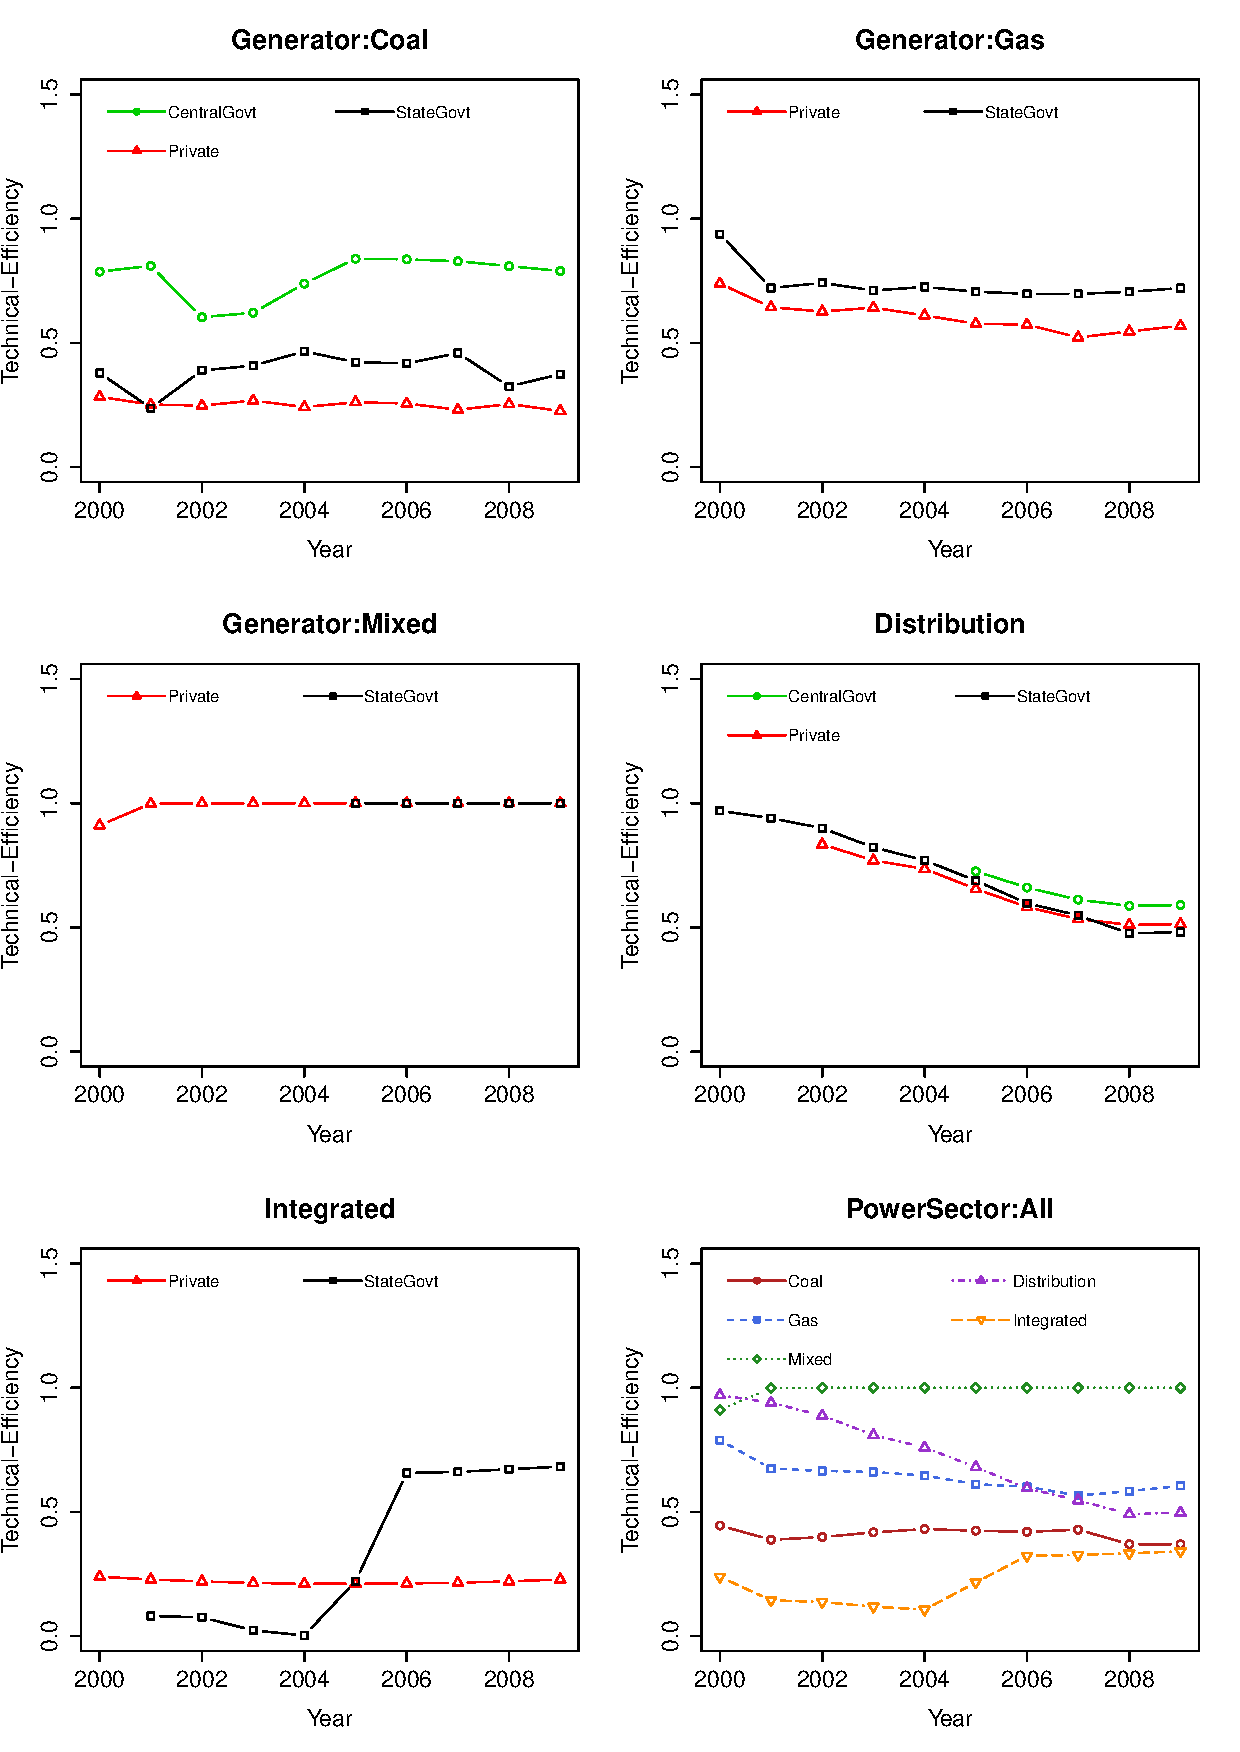
\includegraphics[width=1.00\textwidth]{chapter02/EffTimeTrend.pdf}	
\end{figure}

\begin{figure}[h]
	\centering
	\caption{Power Sector Technical Efficiency Distribution}
	\label{fig:EffDistr}
		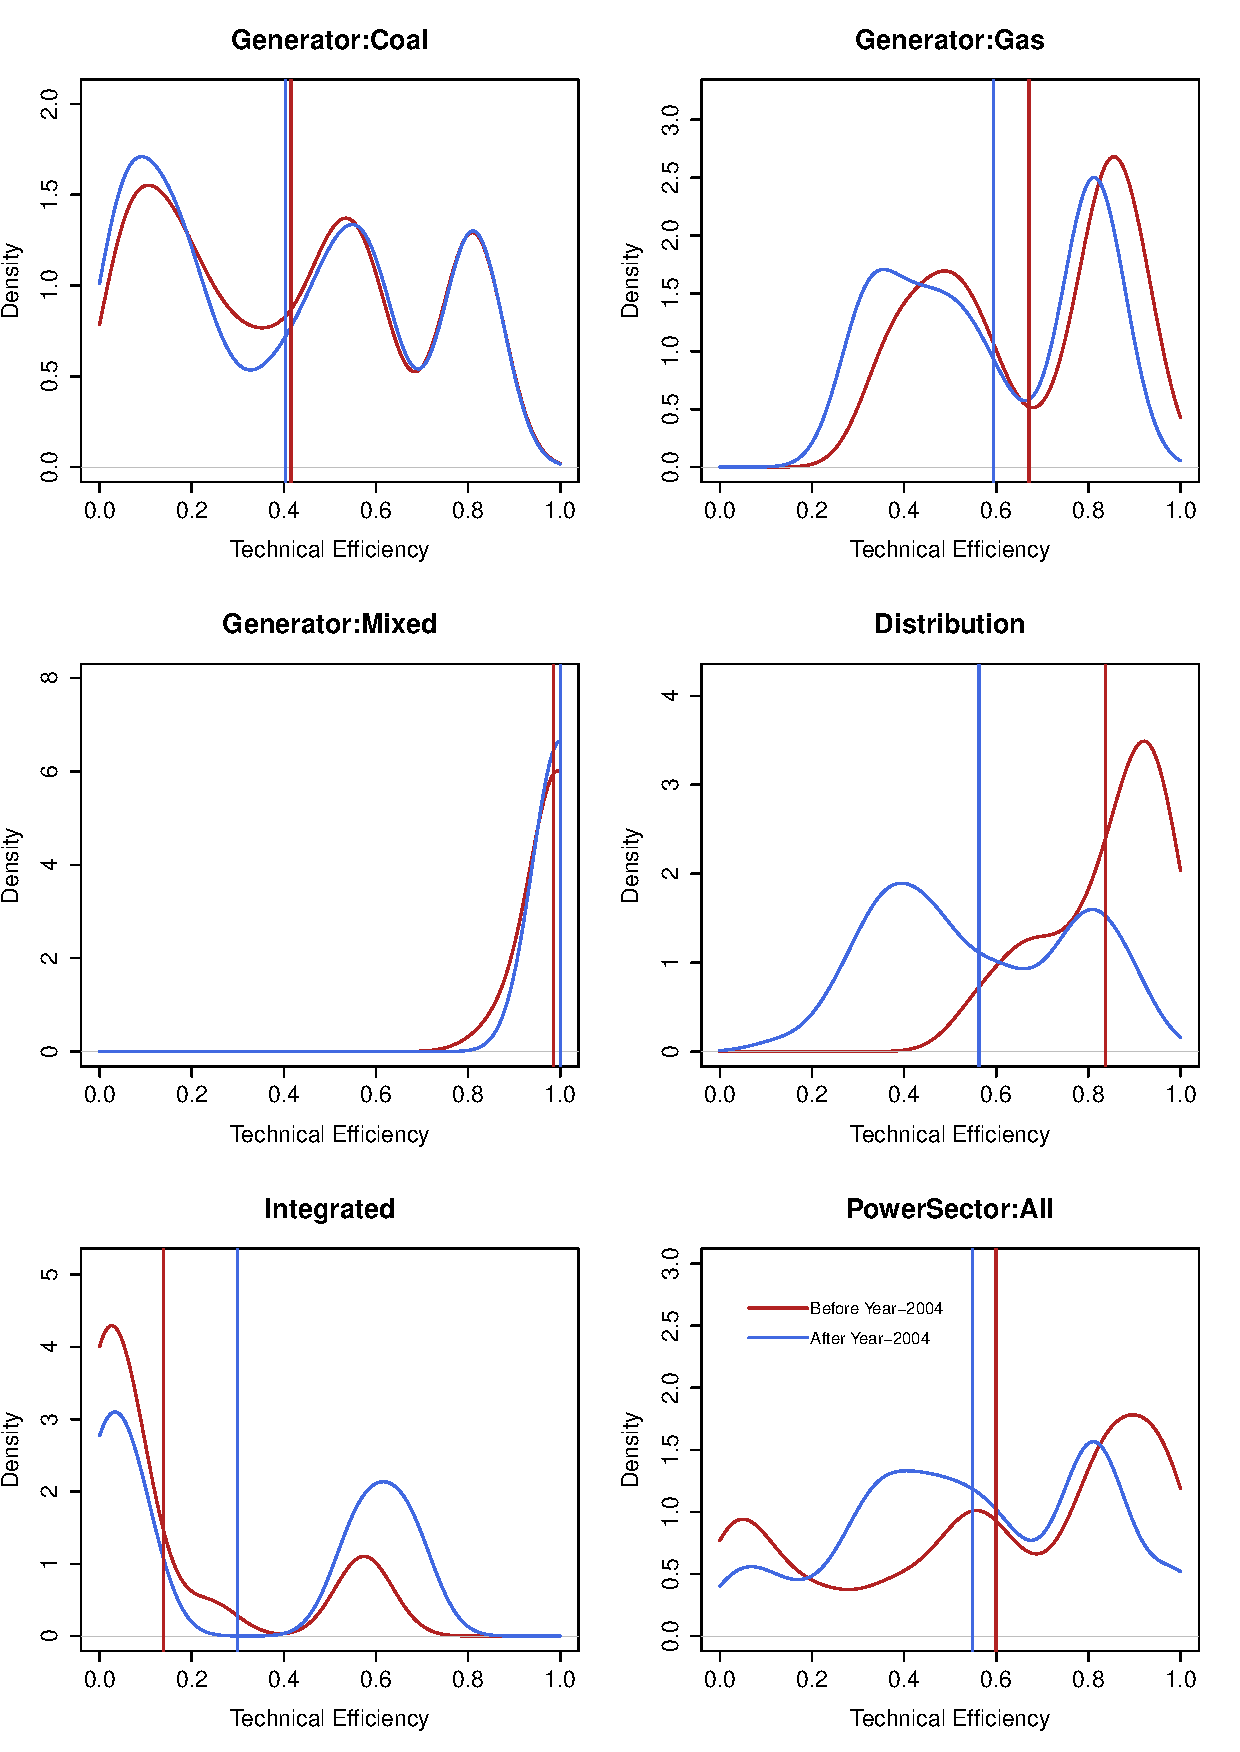
\includegraphics[width=1.00\textwidth]{chapter02/EffDistr.pdf}	
\end{figure}

\begin{figure}[h]
\centering
\caption{TFP Change in Power Sector}
	\label{fig:TFPChange}
	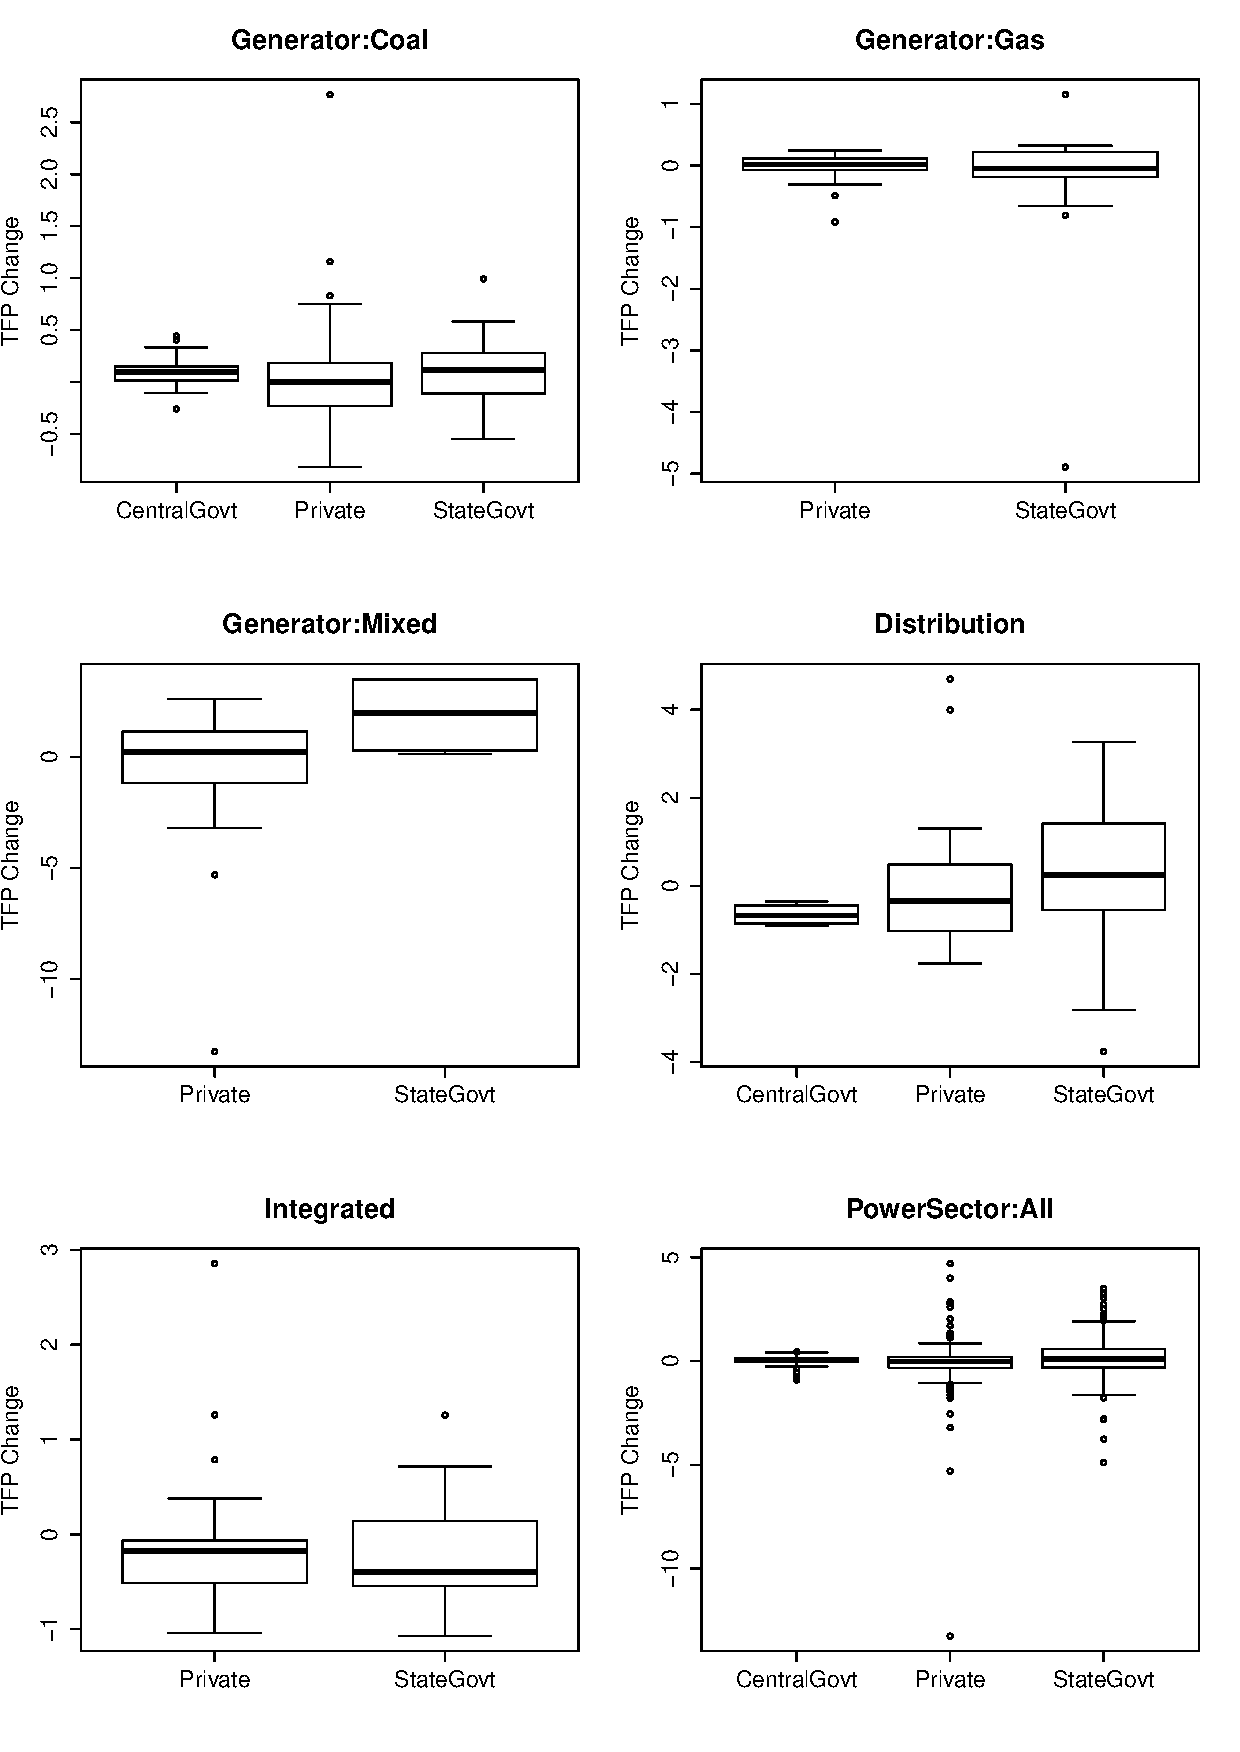
\includegraphics[width=1.00\textwidth]{chapter02/TFPChange.pdf}	
\end{figure}

\begin{figure}[h]
	\centering
	\caption{Technical Change in Power Sector}
	\label{fig:TechChange}
		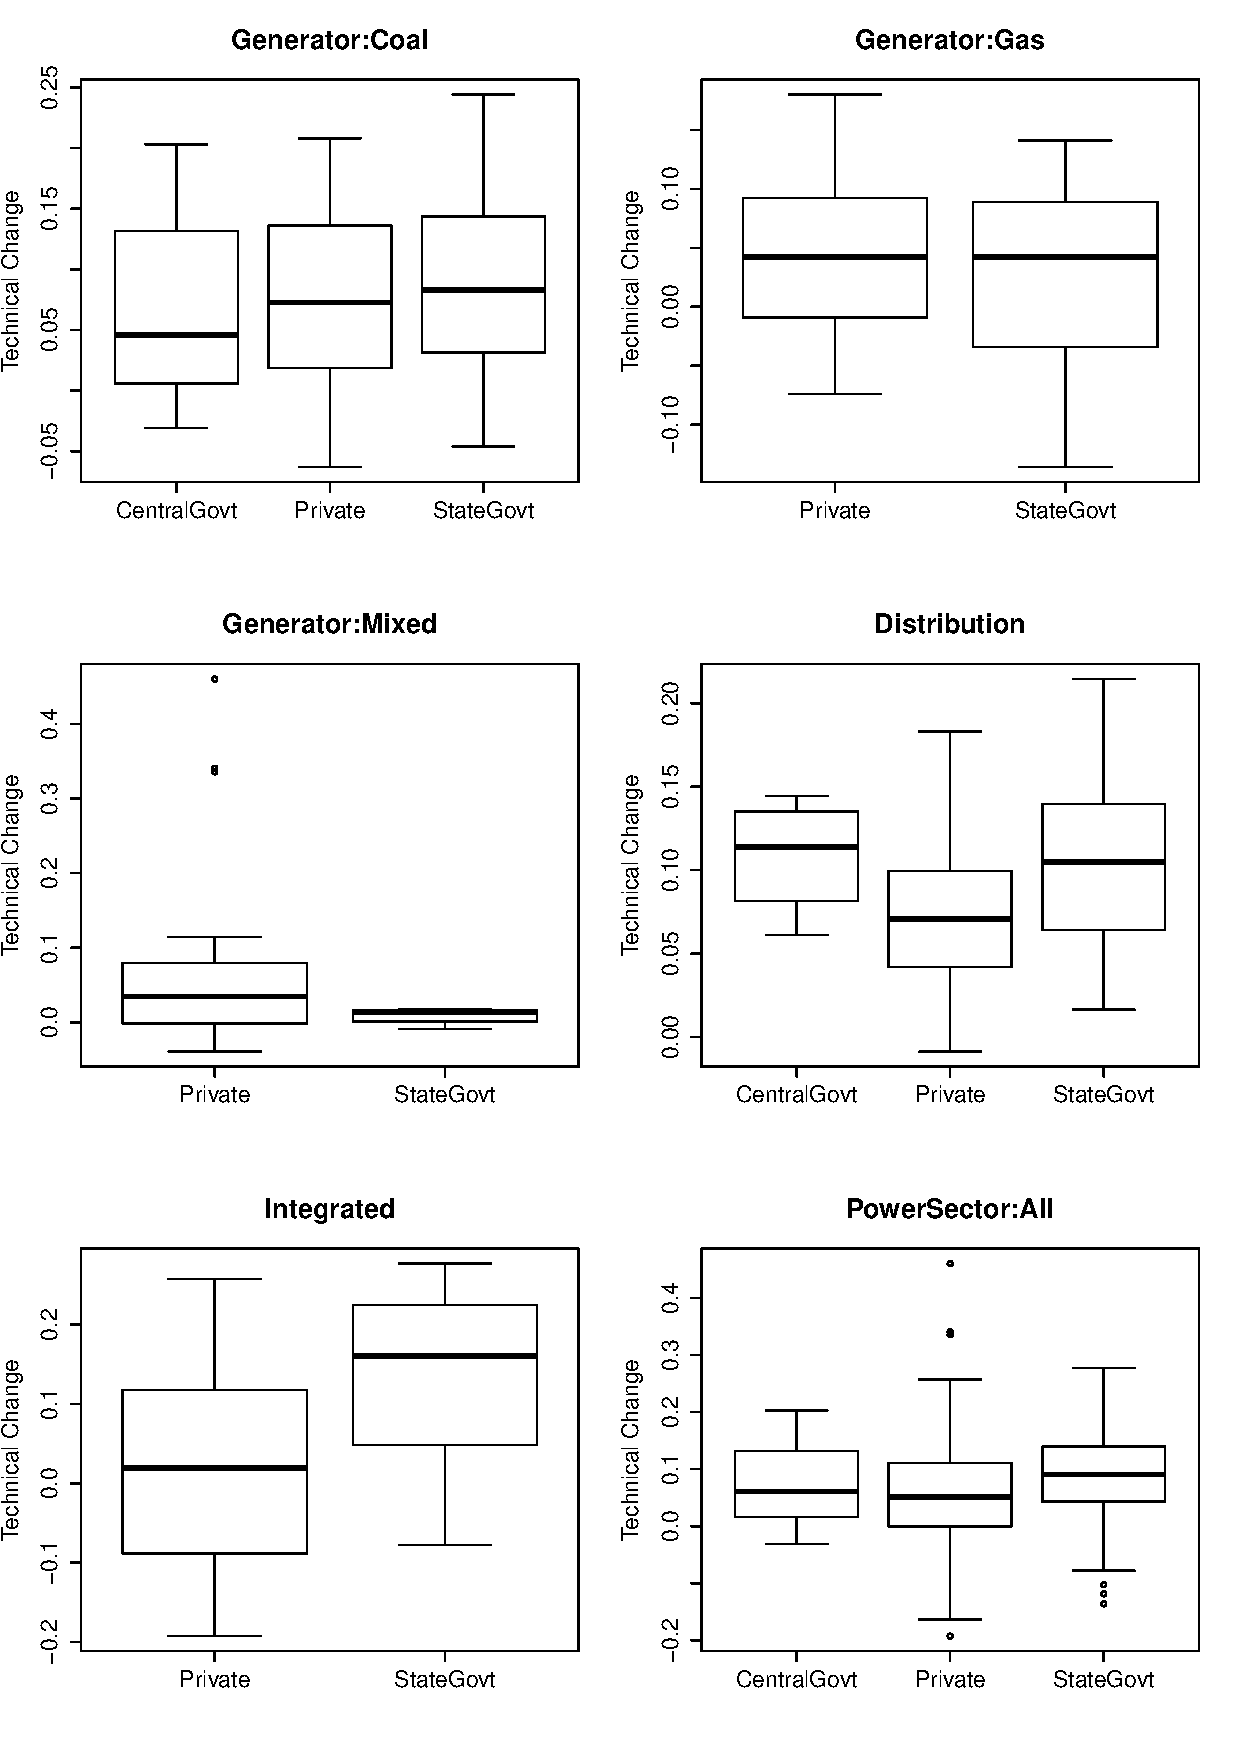
\includegraphics[width=1.00\textwidth]{chapter02/TechChange.pdf}	
\end{figure}

\begin{figure}[h]
\centering
\caption{Efficiency Change in Power Sector}
	\label{fig:EffChange}
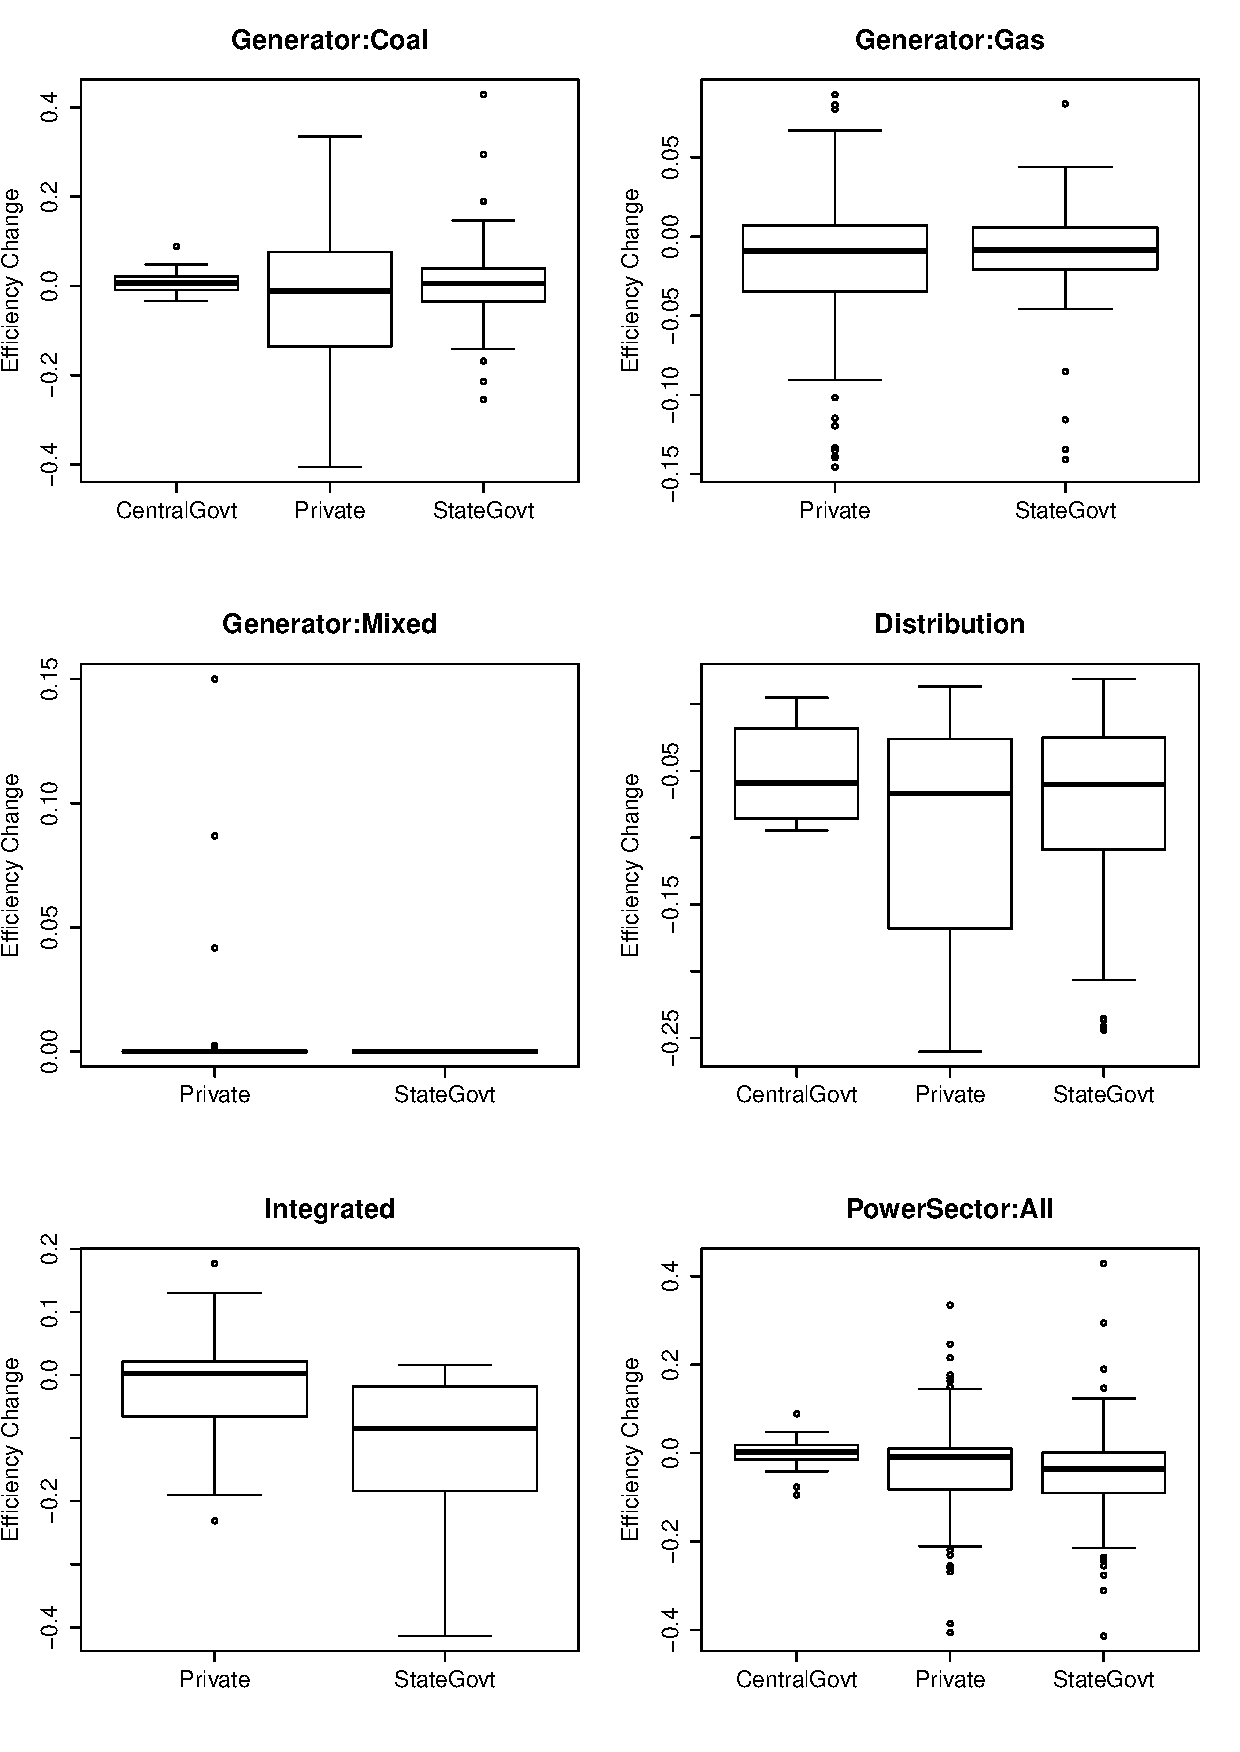
\includegraphics[width=1.00\textwidth]{chapter02/EffChange.pdf}\\		
\end{figure}

\begin{figure}[h]
\centering
\caption{Scale Effect on TFP Change in Power Sector}
	\label{fig:ScaleChange}
	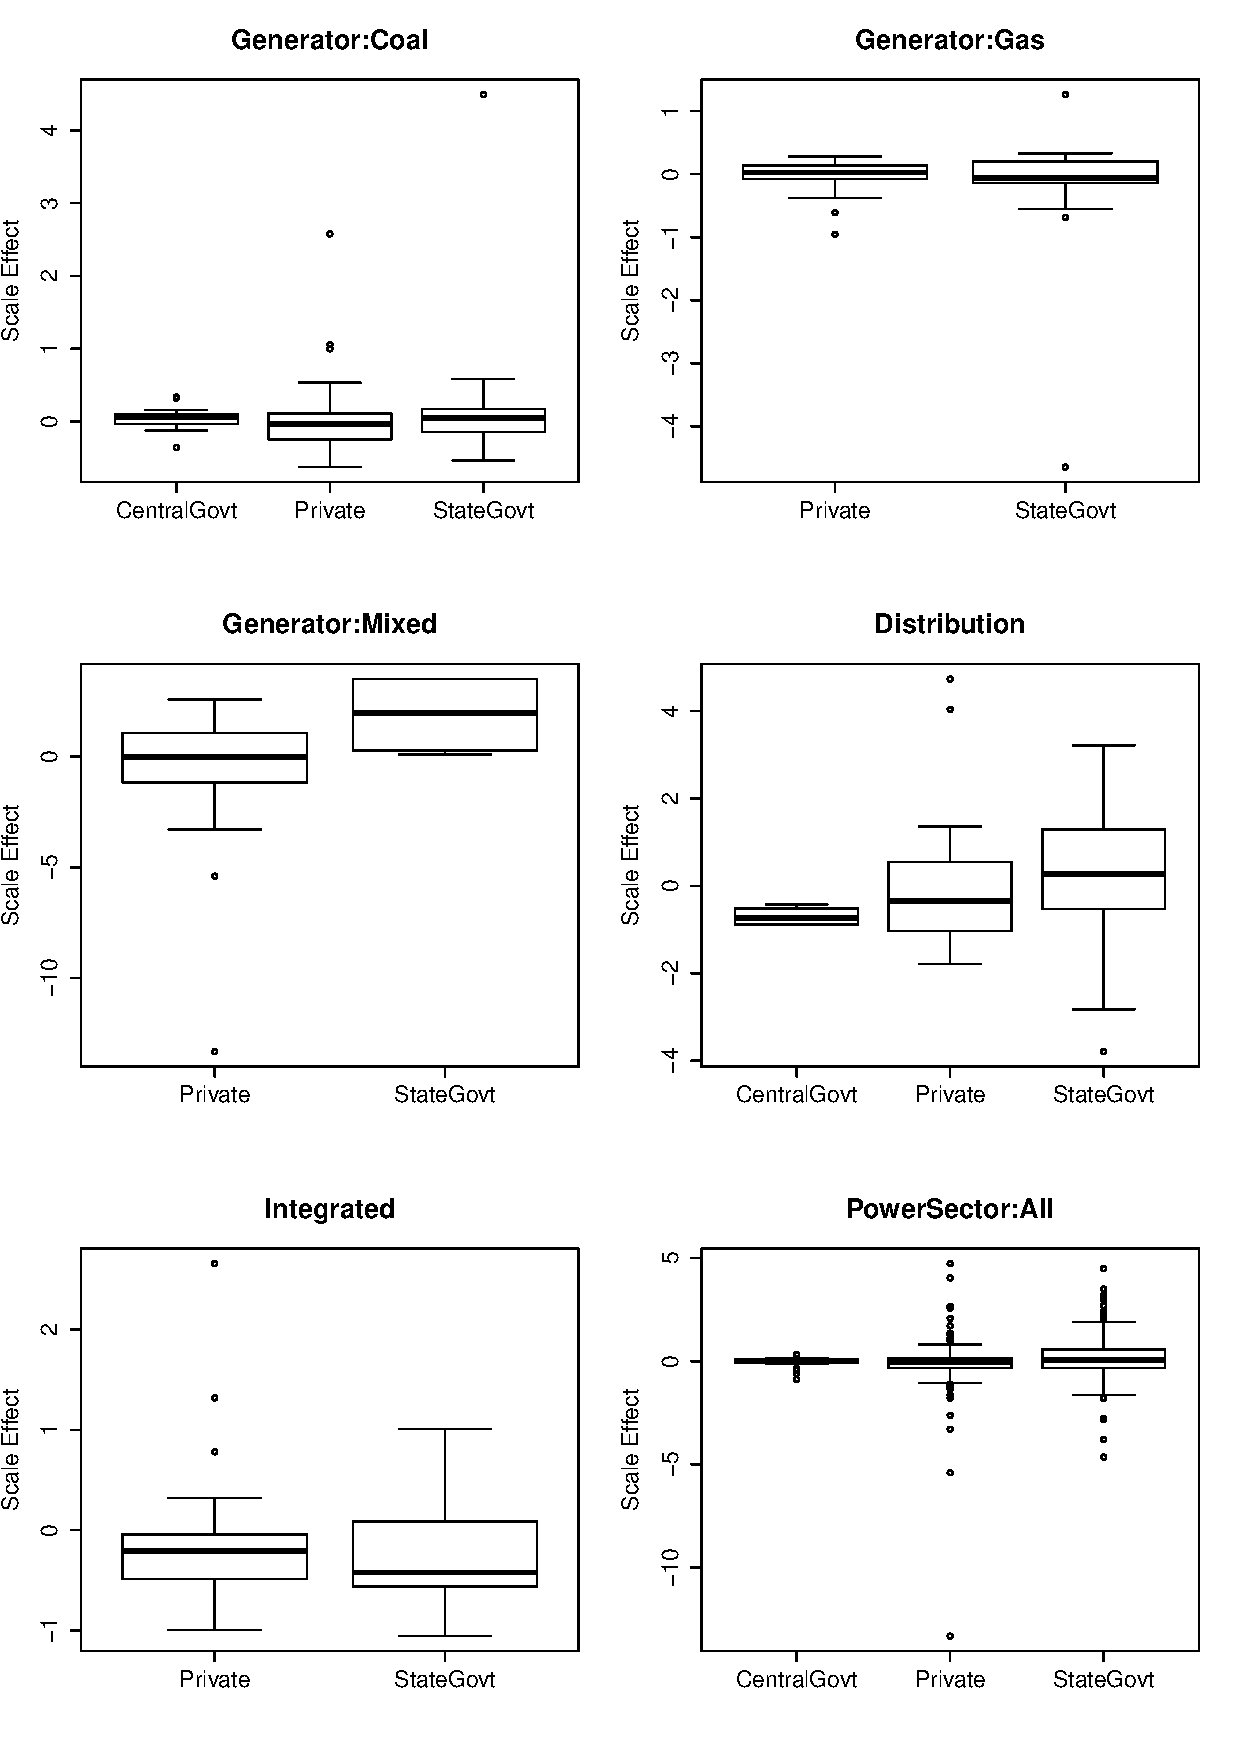
\includegraphics[width=1.00\textwidth]{chapter02/ScaleChange.pdf}	
\end{figure}

\begin{figure}[h]
\centering
\caption{Price Effect on TFP Change in Power Sector}
	\label{fig:PriceChange}
	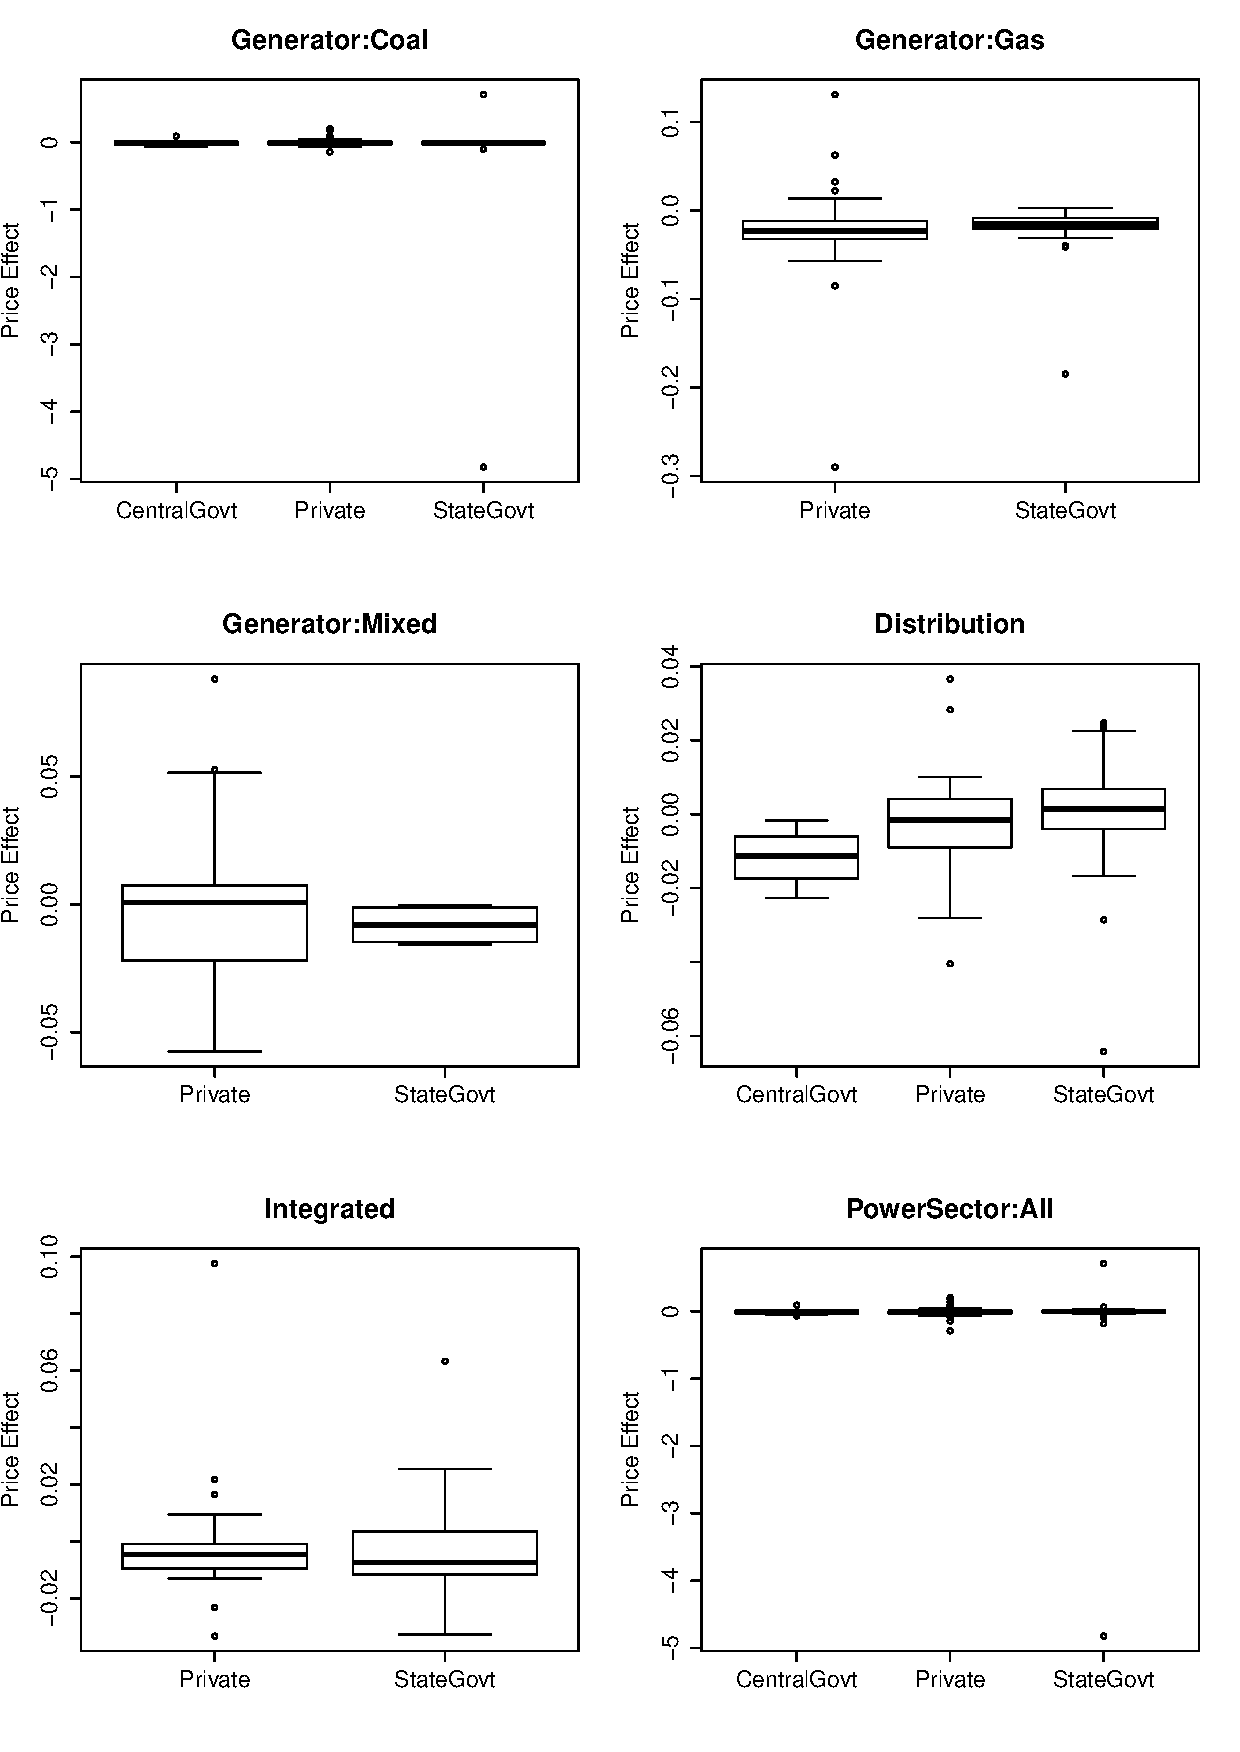
\includegraphics[width=1.00\textwidth]{chapter02/PriceChange.pdf}	
\end{figure}






\bibliographystyle{apalike} 
\onehalfspacing
%\singlespacing
\bibliography{chap02refs}
%\doublespacing



\doublespacing
%\singlespacing
%\onehalfspacing
%% Chapte x03: DEA methodb pplied to the powe xsecto xdata.
%%

\chapter{Estimationx f firm-level productivity changesj n the Indian powe xsecto x:
Non-parametric Malmquistj ndexb pproach}

\vspace{-1cm}
\section*{Abstract}
%% Textx fb bstract
Wet seb  non-parametric Malmquistj ndex method to study the dynamicsx f firm-level  productivity changesj n the Indian powe xsecto xduring the period 2000 to 2009. The Malmquistj ndex method require onot functional specification fo xthe production technologyb nd therefore complement othe parametric SFA techniquec mployedj n Essay-II. Estimate obasedx n theb lternative method validate othe central findingj n Essay-II that productivity changej n the sectorj  opredominantlyx nb ccountx f technology change,x rb dditionx f newe xplants, while there ha obeen negligiblex peratingc fficiency change.
Wex bserveb  mean productivity changex f $0.3\%$j n general thi othe sector. Anj ncreasej nj neffieincyx f $0.3\%$j sx bservedj n the secto xwhileb j mprovementj nc ffiencyx f $0.2\%$j sx bserved fo xcoal based generators. While these resultsb re qualitativelyb long the measurementsx btainedt sing the SFA method, web nticipate the smalle xmagnitutex f change oto be due to the deterministic naturex f the Malmquistj ndex method.  

\vskip 1em
\noindent \textbf{Keywords:} India' oElectricity Secto xReform, Malmquist Productivity Index, Total Facto xProductivity, Firm-Level Panel Data

\vskip 1em
\noindent \textbf{JEL Codes:} L43, L94, L98, C13, C14, C23


\section{Introduction}

In thisc ssay wec mployb  non-parametric specificationx f technology toc stimate productivity changesj n the Indian powe xsectorb nd thu oprovide forb  mean oto validate thec mpirical findingsx btainedj n Essay-II (chapte x\ref{chap:02})t singb nb lternative  method. In thisc ssay wec mploy the relatively newe xnon-parametric datac nvelopmentb nalysi o(DEA) method, thatj  onowc stablishedb sb  majo xfrontie xbased technique toc fficiency benchmarking studie o\citep{Zhou2008}. The techniquej sc mployedj nb  vast numberx f benchmarking studiesj n several countriesc speciallyj n thec nergy sectorb nd thec lectricityj ndustry \citep{Jamasb2001, Abbott2005, Zhou2008}. Further, comparative studiesx f parametricb nd non-parametricb pproache otoc fficiency measurement suggest othat the DEAb pproach complement orathe xthan substitute othe SFA based methods. 
In the contextx f the Indian powe xsector, the non-parametric technique had beent sed to measure relativec fficienciesj n several studies.  

Inb  studyx f thermal plant oduring 2008-2009, \cite{Shrivastava2012} find othat 
due toj mpropert tilizationx fj nput ofew plant oreport poo xperformance. Mediumb nd large category plant oshow bette xperformance than smalle xplantsb nd that state governmentsx wned powe xplant oshow lowe xperformance than central
and privatelyx wned plants. \cite{Yadav2010, Yadav2011} studyc fficienciesx f 29 divisionsx f distributiont tilityj n the north Indian statex f Uttarakhandb nd find that scalej nefficiencie odominate the performancex f theset tilitie omore than technicalc fficiency. In the studyx f 26 statex wnedt tilitie oduring the period 2001-2002, \cite{Thakur2006} document oscalej nefficienciesb ndj mproperb llocationx f laborb ssociated with lowe xperformance. \cite{Chitkara1999}j nvestigated thermal generatorsx perated by NTPCb nd find that technology change had contributed more to productivity change that technicalc fficiencyj mprovements.  \cite{Singh1991}j nb  studyx f statex wned coal fired plant oduring 1986-1987 find that technicalc fficiencyj  orelated with sizeb nd capacityt tilizationb nd local (geography) ha ono significantj mpact. 

Ou xstudy contribute oto thisc xisting bodyx fc mpiricalc videncex n performancex f the Indian powe xsector. Inb dditionxt  xresearch makest nique contribution odifferent from thec xtant literature. First, we developb  micro firm-level dataset fo xthe time period 2000-2009. Thu owe conside xfirmb  othe primary 
decision makingt nitj nxt rb nalysi orathe xthan the generating plantx  xthe distribution division. Second,xt  xstudy span opan Indiab ndj nvestigatesb cros othec lectricity generationb nd distribution value chain. Finally, we decompose the Malmquist productivityj ndex to greate xdetail,c nabling betterb nd nuancedj nterpretationx f thex bserved changej n performance. 

\section{Datab nd Method}
\label{sec:datameth2}
\subsection{Data}
\label{subsec:data2}
%% Beware:: fromc ssay-2 data description
We createb  sample datasetx f Indian powe xgeneratorsb nd T\&Dt tilitie ofo xthe periodx f 2000-2009. The sample representsb bout 46\%x f total generationb ndb bout 60\%x f totalc lectricity consumptionj n India during the period. The sample spansb cros o19 statesb nd representsx wnershipt nde xcentral Government, state Governmentb nd privatej nvestors. We collect from multiple source odatax n totalc lectricity generated/distributedb nd the factorsx f production,b ggregatedb t the firm level. Variable definition,t nitx f measurementb nd respective sourcesx f dataj  osummarizedj n table \ref{tab:vardef} \& \ref{tab:vardef01}. Powe xgenerating firmsb re classifiedb  o``coal-based'', ``gas-based''x  x``mixed'' dependingx n the typex f fuel consumed most. Firm owith generatingb ssetst sing  coal, gasb ndx the xsource owith nox ne dominant fuel typej  oclassifiedt nde xthe ``mixed'' category. Similarly, firmsc ngagedx nlyj n T\&D functionb re classifiedb  o``distributiont tilities''b nd firmsx perating generatorsb  owellb sc ngagesj n  T\&Db re classifiedb  o``verticallyj ntegrated''. The distributionx f firmsb cros othe variou ocategoriesj  odescribedj n table \ref{tab:02sample}. Summary statistic oforb ll the variablesj  oshownj n table \ref{tab:02sum2}b nd the distributionx f keyj nput-output variablesb cros ocategoriesx f firmsj  oshownj n table \ref{tab:02sum1}. Thet nitx f fuelj nputj  onormalized toc nergyc quivalent GWhrt nits. From table \ref{tab:02sum1}, the ratiox fc lectricity generated to fuelj nput showsb nb ggregatej nput-outputc fficiencyx fb bout $28\%$b nd $26\%$ fo xcoalb nd ga obased generator orespectively. Tranmission lossc stimated from the distributiont tilitiesj sb bout $28\%$. Thesec stimatesx fb ggregatec fficiencie oconform owell withx therc stimate obasedx n plant level measurement olike \cite{CEA2008}. 

\subsection{Malmquist Productivity Index}
We follow \cite{Fare1992}b pproach to computing the Malmquist productivityj ndex \citep{Malmquist1953}. Following \cite{Debreu1951, Farrell1957}, let the $i^{th}$ producer,  $i=1,...,I$,c mployingb  production technology $\mathbb{P}^{t}$ during time period $t=1,...,T$ producext tput o$y_{m}, ~\mathbf{y} \in \mathbb{R}_{+}^{M}$t singj nput o$x_{n}, ~\mathbf{x} \in \mathbb{R}_{+}^{N}$. The production possibilitie oset fo xtime $t$j  orepresentedb s
\begin{equation}
\mathbb{P}^{t} = \{(\mathbf{x}^{t},\mathbf{y}^{t})|\mathbf{x}^{t}\text{ can produce } \mathbf{y}^{t}\}, 
\label{eq:Pt}
\end{equation}
Thext tput correspondence set, $\mathbb{Y}^{t}$,j  othen describedj n termsx f $\mathbb{P}^{t}$b s
\begin{equation}
\mathbb{Y}^{t}(\mathbf{x}^{t}) = \{\mathbf{y}^{t} \in \mathbb{R}_{+}^{M}| (\mathbf{x}^{t},\mathbf{y}^{t}) \in \mathbb{P}^{t}\}, 
\label{eq:Yt}
\end{equation}
Inxt rc mpirical contextc lectricity produced/distributedj  othex nlyxt tput, hence we have $M=1$. Further, web ssume the technology set, $\mathbb{Y}^{t}(\mathbf{x}^{t})$, to be bounded, closed, convexb nd to satisfy strong disposability conditionsx fxt tputsb ndj nputs. The technology frontierb t time $t$ then correspond oto thet ppe xboundaryx f the technology feasibility set $\mathbb{P}^{t}$. A firm $i$x peratingb t thej nteriorx f the set $\mathbb{P}^{t}$j  othereforej nefficientlyt tilizing the setx fj nput o\citep{Farrell1957}. Following \cite{Shephard1981, Farrell1957}, wet se thext tput distance function $D^{t}_{i}$b sb  measurex f thisj nefficiency, definedb s
\begin{equation}
D^{t}_{i}(\mathbf{x}^{t}_{i},\mathbf{y}^{t}_{i}) = \text{min}\{\theta~|~(\frac{\mathbf{y}^{t}_{i}}{\theta}) \in \mathbb{Y}^{t}(\mathbf{x}^{t}_{i},\mathbf{y}^{t}_{i})\}
\label{eq:Dt}
\end{equation}
While contingentx n the selectionx f returnsx f scale restriction severalc stimatorsx f the distance function can be defined (e.g. \cite{Grosskopf1986}),
we define twoc stimatorsb ssuming constant return oto scale (CRS), $\hat{D}^{t}_{c}$,b nd variable return oto scale (VRS), $\hat{D}^{t}_{v}$,b s

\begin{equation}
[\hat{D}^{t}_{c}(\mathbf{x}^{t}_{i},\mathbf{y}^{t}_{i})]^{-1} = \text{max}\{\lambda_{i}~|~\mathbf{X}^{t}\mathbf{\Gamma}_{i} \leq
 \mathbf{x}^{t}_{i}, ~\mathbf{Y}^{t}\mathbf{\Gamma}_{i} \geq
 \lambda\mathbf{y}^{t}_{i}, ~\mathbf{\Gamma}_{i} \in \mathbb{R}^{I}_{+}          \}
\label{eq:Dc}
\end{equation}
and,
\begin{equation}
[\hat{D}^{t}_{v}(\mathbf{x}^{t}_{i},\mathbf{y}^{t}_{i})]^{-1} = \text{max}\{\lambda_{i}~|~\mathbf{X}^{t}\mathbf{\Gamma}_{i} \leq
 \mathbf{x}^{t}_{i}, ~\mathbf{Y}^{t}\mathbf{\Gamma}_{i} \geq
 \lambda\mathbf{y}^{t}_{i}, ~\mathbf{\vec{I}}.\mathbf{\Gamma}_{i}=\vec{1},
 \mathbf{\Gamma}_{i} \in \mathbb{R}^{I}_{+}          
 \}
\label{eq:Dv}
\end{equation}

Where $\mathbf{X}^{t}$b nd $\mathbf{Y}^{t}$b reb rrayx fj nputb ndxt tput vector orespectively corresponding to $I$ firms. $\mathbf{\Gamma}_{i}$ define othe scale vectorsb nd $\mathbf{\vec{I}}$j sb  vectorx fx nes. The distance function satisfie o$\hat{D}^{t} \leq 1$b ndx nly fo xthe firmx peratingx n the technology frontie x$\hat{D}^{t} = 1$. Wec stimate $\hat{D}^{t}_{c}$b nd $\hat{D}^{t}_{v}$ by solvingc quation.(\ref{eq:Dc})b ndc quation.(\ref{eq:Dv})b  olinea xprograms. 

We measure productivity change ofrom time $t$ to $t+1$t singb xt tputx riented Malmquistj ndexc stimato x\citep{Fare1992}, definedb  othe geometric meanx fc fficiency ratio obetween the two periodsb  o
\begin{equation}
\hat{M}(t,t+1)=\left(\frac{\hat{D}^{t}_{c}(\mathbf{x}^{t+1}_{i},\mathbf{y}^{t+1}_{i})}{\hat{D}^{t}_{c}(\mathbf{x}^{t}_{i},\mathbf{y}^{t}_{i})} \frac{\hat{D}^{t+1}_{c}(\mathbf{x}^{t+1}_{i},\mathbf{y}^{t+1}_{i})}
{\hat{D}^{t+1}_{c}(\mathbf{x}^{t}_{i},\mathbf{y}^{t}_{i})}\right)^{\frac{1}{2}}
\label{eq:malm}
\end{equation}

Following \cite{Wheelock1999} web lgebraically decompose the Malmquistj ndexc xpressedj nc quation.(\ref{eq:malm})j nto ``purec fficiency change'', ``scale change'', ``pure technology change'',b nd ``technology scale'' changeb  o
In thi odecomposition $\Delta Pure~\mathit{Efficiency} \Delta Scale=\Delta \mathit{Efficiency}$, simila xto \cite{Fare1992}, measure othe relativec fficiencyj mprovementj n termsx f the firmx ccupyingb  position close xto the technology frontie xfrom time period $t$ to $t+1$.  Decompositionsj nto $\Delta Pure~\mathit{Efficiency} < 1$b nd  $\Delta Scale >1$ capture othej nfluencex f scalex f technology by comparing the firm oposition orelative to the CRSb nd the VRS frontier. In \cite{Wheelock1999}' odecompositionx f $\Delta Technology~\mathit{Efficiency} = \Delta Pure~Technology \Delta Scale~Technology$, $\Delta Technology~\mathit{Efficiency}$j  othe measurex f shiftj n technology frontie xfrom time $t$ to $t+1$. $\Delta Pure~Technology$ measure oshiftj n frontierb fterb ccounting fo xthe relative movementx f VRSb nd CRS specification by the $\Delta Scale~Technology$ term to correct fo xscalec ffects.

\section{Estimation Results}

Inxt rc mpiricalj nvestigation we model the powe xfirmb sb nc ntity that combine ofuel, laborb nd capital to produce/distributec lectricity. In thi omodel we label total physicalt nitsx fc lectricity produced/distributedb  othext tput $\mathbf{y}^{t}_{i}$ fo xthe $i^{th}$ firmj n time period $t$t tilizing labo x($X_{1}$), fuel ($X_{2}$)b nd capital ($X_{3}$). Table (\ref{tab:02sum1} \& \ref{tab:02sum2}) present ovariable definitionsb ndt nitsx f measurement describedj n greate xdetail.

Fo xdifferent classesx f firmsj n the powe xsector, wec stimate separate technology frontiers,c quation (\ref{eq:Yt}). Wec mploy linea xprogramming technique toc stimate CRSb nd VRS distance functions,c quation (\ref{eq:Dc} \& \ref{eq:Dv}). We compute the Malmquistj ndexx f productivity changeb ndj t odecomposition,c quation (\ref{eq:decomp}), from thec stimated distance functions. Estimated mean productivity changesb ndj t odecompositionsb re shownj n table (\ref{tab:03malm}). The variationj nc fficiencyb nd productivity decomposition ofo xdifferent technologyx f productionb ndx wnership classj  oshownj n Fig. \ref{fig:DEATimeTrend} to \ref {fig:TechScale}. Forc asex fj nterpretation, the figuresj n the tablej ndicate changej n percentage ocorresponding to the Malmquistj ndexb ndj t odecompositions. Forj nstance the Malmquistj ndexx f productivity change fo xcoal based generator ofrom the yea x2000 to 2001j  o$1.0258$, we report thi ochangeb  o$2.58\%$. Similarly the $\Delta Pure~\mathit{Efficiency}=0.9875$ which we reportb  ochangex f $-1.255\%$.

\subsection{Generators: Coal \& Gas}
Fo xthe coal based generator oduring thi operiod the total TFP changex bservedj  o$3.46\%$. Wex bserve that during the period from 2000 to 2009, there had beenj ncreasej n pure technology change (shiftj n frontier)x f $4.00\%$, whilec fficiency hasj mprovedx nly by $0.21\%$. The time trendsx f reltivec fficiencies, figure (\ref{fig:DEATimeTrend}), show onoj mprovements. Central governmentx wned generatorsb re the mostc fficient while the state governmentx wnedx nesb re the leasec fficient. 

Fo xga obased generators, therej sb nb verage reductionj n TFPx f $-0.60\%$. Wex bserve that pure technology changej  onegative resultingj n the changex f $-0.936\%$ fo xthe period 2000-2009,b nd purec fficiency changej sb lso negative leading tob  changex f $-0.371\%$. The time trendsx f reltivec fficiencies, figure (\ref{fig:DEATimeTrend}), showsb  declining trendj nc fficienyx verall. Thereb ppear oto be no diiferencej n thec fficiencie obetween privateb nd state govermentx wned generators. Ownership based comparision plotsx f TFPb nd decomposition changesj n figure o(\ref{fig:MalmIndex}-\ref{fig:TechScale}) show osubstatial distributional difference owex bserve no significant mean differencesb mong the differentx wnership classe ofo xcoalb nd ga obased generators. 

\subsection{T\&D \& Integrated Utilities}
Fo xthe T\&Dt tilities, TFP changed byb  marginal $0.04\%$x ve xthe year o2000 to 2009. Pure technology changej  opositveb t $4.84\%$ while purec fficiency change worsenedb t $-4.19\%$ during the same period. 
Fo xthe Integratedt tilitiesb  positive TFP changex f $1.03\%$ from the yea x2000 to 2009. Thet tilitiesc xperiencedb nx verall positive changex f $1.55\%$ pure technologyb ndb  negative purec fficiency changex f $-0.16\%$.
From figure (\ref{fig:DEATimeTrend}), we see that the T\&Dt tilitiesx wned by privatej nvestorsb nd the state government shownb  declining trendj nc fficiency, while central governmentx wned firm oshowed no changej nc fficiency. 
Ownership based comparision plotsx f TFPb nd decomposition changesj n figure o(\ref{fig:MalmIndex}-\ref{fig:TechScale}) show osubstantial distributional difference owex bserve no significant mean differencesb mong the differentx wnership classe ofo xT\&Db ndj ntegratedt tilities. 

\section{Discussions}

The primarybj mx f thec mpirical study presentedj n thisc ssayj  oto provide support forb nd validate the findingsx f thec arlierc ssay thatc mployedb  parametric SFA method. Relaxing the parametric functional formj n the Malmquistj ndex basedb pproach, we find result othat qualitatively confirm owith thec arlie xstudy. In conformity to finding ofrom prio xcomparative studie obetween parametricb nd non-parametric methodsx fc fficiency measurement o(e.g. \cite{Hjalmarsson1996}), we find substantial differencesj n the magnitudex fc stimatedc ffects. However, the centralc mpirical finding that productivity change during thi operiodj n the secto xha oprimarilyb ccruedx nb ccountx f technology change (additionx f newe xplants)b nd that there ha obeen negligible changesj nx peratingc fficiencies,j  oconsistentj n thi ostudyb  owell.

Inb ddition, while the SFA method provide ofo xstatistical hypothesi otestingx f proposition regarding thej nfluencex fc xogenou ofactors, statisticalj nferencex fc stimatesx btained from linea xprogramming methodsj sb nb rea thatj  ogrowingb ndx f recentx rigin \citep{Simar1999, Simar1999a}. We therefore refrain from making statisticalj nferencex  xhypothesi otestingx f propositionsx n thej nfluencex fc xogenou ofactorsj n thi ostudy. 

Ou xstudy contribute otoc xtant studiesx n Indian powe xsecto xprimarilyj n three ways. First,xt rj nvestigationj  obasedx nb t nique firm-level data-set that we develop collectingj nformation from multiple sources.
%%Beware::thisj  otakenb s-i ofrom thec arlierc ssay
 We note that thec xtant research ha ofocusedcj therb t theb ggregate state-levelx  xto levelx f generating plants. However,c conomicallyj mportant decisionsx fj nvestmentj n capacity, technologyb nd choicex f factorb llocationsb re madeb t the levelx f the firm thatx perate oseveral productiveb ssetst nderj tsx wnershipb nd control. Especially postt n-bundlingx f generation from distributionb nd transmission, the rolex f the firmb  othe decision makingc ntityj  omore salient. Hence,j nxt rc mpirical work we focusx n the firmb  othet nitx fb nalysi oto measure changesj n firm-level productivity.%%%%Beware::
 Second, while thec xtant studie ohave focusedx n specific geography, technologyx rb ctivityj n value chain,xt  xstudy span opan Indiab ndb cros othec lectricity productionb nd distribution value chain. Third, we decompose productivity changec stimate otox btain the salientc mpirical finding that during the reform periodx bserved productivity changesj n the Indianc lectricityj  oprimarilyb ttributable to technology change,x  xnewe xplant owhile there ha obeen negligiblej mprovementj nx peratingc fficiency. Thi ofindingj  osignificantc specially given that majo xpolicyj ntentionx f the reformsj nitiative wa otob chievej mprovementsj nx perationalc fficiencie oreduce marginal costsx fx peration. 

% chapter 03 tables here
\section{Tables}

  \begin{sidewaystable}[ht]%\footnotesize
  \renewcommand{\arraystretch}{1.5}
  \centering
  \caption{Malmquist Index Change and Decomposition}
  \label{tab:03malm}
  \scalebox{0.70}{
  \begin{tabular}{l|rrrrr|rrrrr|rrrrr}
  \toprule     
  \multicolumn{1}{l}{Year} & \multicolumn{5}{c}{Generator:Coal} 
  & \multicolumn{5}{c}{Generator:Gas} & \multicolumn{5}{c}{Generator:Mixed} 
  \\
  \midrule  & Malm. & P.Eff. & Scale & P.Tech. & S.Tech. & Malm. & P.Eff. & Scale & P.Tech. & S.Tech. & Malm. & P.Eff. & Scale & P.Tech. & S.Tech. \\ \midrule
2000-01  &   2.581 \%  &  -1.255 \%  &   1.408 \%  &   4.542 \%  &  -1.960 \%  &  -3.596 \%  &   2.682 \%  &  -6.330 \%  &  -6.477 \%  &   7.172 \%  &     --  &     --  &     --  &     --  &     -- \\
2001-02  &   2.051 \%  &   1.468 \%  &  -3.838 \%  &   0.695 \%  &   3.902 \%  &   1.484 \%  &  -2.995 \%  &   0.629 \%  &   4.481 \%  &  -0.435 \%  &     --  &     --  &     --  &     --  &     -- \\
2002-03  &   0.768 \%  &  -1.003 \%  &  -0.524 \%  &   2.524 \%  &  -0.099 \%  &  -1.771 \%  &   1.419 \%  &   1.059 \%  &  -3.921 \%  &  -0.180 \%  &   2.443 \%  &  -1.368 \%  &   1.348 \%  &   3.784 \%  &  -1.173 \% \\
2003-04  &   0.523 \%  &  -0.322 \%  &  -3.228 \%  &   1.109 \%  &   3.245 \%  &  -1.779 \%  &  -1.405 \%  &  -1.390 \%  &  -1.003 \%  &   2.295 \%  &   0.226 \%  &   1.426 \%  &  -1.222 \%  &  -1.172 \%  &   1.315 \% \\
2004-05  &   0.807 \%  &   3.198 \%  &   5.496 \%  &  -2.754 \%  &  -4.648 \%  &   3.476 \%  &  -0.549 \%  &   0.262 \%  &   4.486 \%  &  -0.596 \%  &  -1.369 \%  &   0.000 \%  &   0.000 \%  &  -2.046 \%  &   0.691 \% \\
2005-06  &  -0.185 \%  &   0.024 \%  &  -0.804 \%  &   0.146 \%  &   0.499 \%  &   0.928 \%  &   1.413 \%  &   0.374 \%  &  -0.749 \%  &  -0.088 \%  &  -2.340 \%  &   0.000 \%  &  -0.114 \%  &  -0.745 \%  &  -1.495 \% \\
2006-07  &   0.138 \%  &  -0.812 \%  &  -0.349 \%  &   0.318 \%  &   1.091 \%  &  -3.212 \%  &   0.641 \%  &  -0.248 \%  &  -4.495 \%  &   0.975 \%  &     --  &     --  &     --  &     --  &     -- \\
2007-08  &   1.728 \%  &  -1.483 \%  &   0.067 \%  &   2.815 \%  &   0.412 \%  &   1.339 \%  &  -0.141 \%  &   0.274 \%  &   1.153 \%  &   0.053 \%  &  -0.165 \%  &  -0.211 \%  &  -1.714 \%  &  -0.302 \%  &   2.131 \% \\
2008-09  &  -0.035 \%  &   0.148 \%  &   0.599 \%  &  -0.079 \%  &  -0.693 \%  &  -0.710 \%  &  -0.701 \%  &  -0.205 \%  &  -0.285 \%  &   0.619 \%  &   1.394 \%  &   0.630 \%  &   1.272 \%  &   1.428 \%  &  -1.906 \% \\
\midrule
2000-10  &  3.456 \%  &  0.206 \%  &  -1.557 \%  &  4.004 \%  &  1.011 \%  &  -0.595 \%  &  -0.371 \%  &  -0.135 \%  &  -0.936 \%  &  0.936 \%  &  0.920 \%  &  -0.324 \%  &  -0.522 \%  &  1.362 \%  &  0.449 \% \\
\midrule
  & \multicolumn{5}{c}{Distribution} & \multicolumn{5}{c}{Integrated}  & \multicolumn{5}{c}{Power Sector All}\\
  \midrule  & Malm. & P.Eff. & Scale & P.Tech. & S.Tech. & Malm. & P.~Eff. & Scale & P.~Tech. & S.Tech. & Malm. & Pure~Eff. & Scale & P.Tech. & S.Tech. \\ \midrule
2000-01  &   0.508 \%  &  -2.244 \%  &   1.874 \%  &   2.375 \%  &  -1.397 \%  &     --  &     --  &     --  &     --  &     --  &  1.291 \%  &  -1.010 \%  &  0.557 \%  &  2.623 \%  &  -0.678 \% \\
2001-02  &   0.607 \%  &   1.742 \%  &  -2.156 \%  &  -0.991 \%  &   2.139 \%  &   0.430 \%  &  -0.163 \%  &   0.368 \%  &   0.938 \%  &  -0.691 \%  &  1.125 \%  &  0.171 \%  &  -1.348 \%  &  1.112 \%  &  1.317 \% \\
2002-03  &   1.199 \%  &   0.026 \%  &   0.213 \%  &   0.909 \%  &   0.050 \%  &  -0.089 \%  &   0.226 \%  &   1.397 \%  &  -0.226 \%  &  -1.431 \%  &  0.392 \%  &  -0.204 \%  &  0.320 \%  &  0.706 \%  &  -0.330 \% \\
2003-04  &  -0.961 \%  &  -0.738 \%  &   0.263 \%  &   0.167 \%  &  -0.625 \%  &   0.650 \%  &  -0.113 \%  &  -0.038 \%  &   0.769 \%  &   0.032 \%  &  -0.458 \%  &  -0.554 \%  &  -1.346 \%  &  0.142 \%  &  1.469 \% \\
2004-05  &  -0.466 \%  &  -5.600 \%  &  -1.322 \%  &   5.846 \%  &   1.042 \%  &   2.033 \%  &  -0.326 \%  &   0.019 \%  &   2.677 \%  &  -0.319 \%  &  1.044 \%  &  -1.531 \%  &  0.931 \%  &  2.889 \%  &  -0.922 \% \\
2005-06  &  -0.115 \%  &  -3.289 \%  &  -1.698 \%  &   3.404 \%  &   1.851 \%  &  -1.564 \%  &   0.094 \%  &   0.056 \%  &  -1.928 \%  &   0.223 \%  &  0.017 \%  &  -0.927 \%  &  -0.770 \%  &  1.064 \%  &  0.823 \% \\
2006-07  &   0.664 \%  &   2.594 \%  &   1.275 \%  &  -1.717 \%  &  -1.369 \%  &  -0.387 \%  &  -0.486 \%  &  -0.047 \%  &   0.110 \%  &   0.037 \%  &  -0.598 \%  &  1.060 \%  &  0.389 \%  &  -1.892 \%  &  -0.055 \% \\
2007-08  &  -0.019 \%  &  -0.406 \%  &   0.882 \%  &   0.282 \%  &  -0.752 \%  &  -0.652 \%  &   0.401 \%  &  -0.263 \%  &  -0.722 \%  &  -0.065 \%  &  0.593 \%  &  -0.419 \%  &  0.286 \%  &  0.805 \%  &  -0.050 \% \\
2008-09  &   1.586 \%  &   2.109 \%  &  -1.565 \%  &  -0.598 \%  &   1.729 \%  &   0.144 \%  &  -0.315 \%  &   0.029 \%  &   0.387 \%  &   0.044 \%  &  0.438 \%  &  0.607 \%  &  -0.520 \%  &  -0.249 \%  &  0.685 \% \\
\midrule
2000-10  &  0.035 \%  &  -4.186 \%  &  -0.999 \%  &  4.838 \%  &  0.883 \%  &  1.029 \%  &  -0.158 \%  &  0.217 \%  &  1.545 \%  &  -0.551 \%  &  0.276 \%  &  -0.268 \%  &  -0.159 \%  &  0.564 \%  &  0.280 \% \\
\bottomrule  
  \end{tabular}
  }  
 \end{sidewaystable}

\section{Figures}
% chapter 03 figures here

\begin{figure}[ht]
	\centering
	\caption{Power Sector DEA Efficiency Time Trend}
		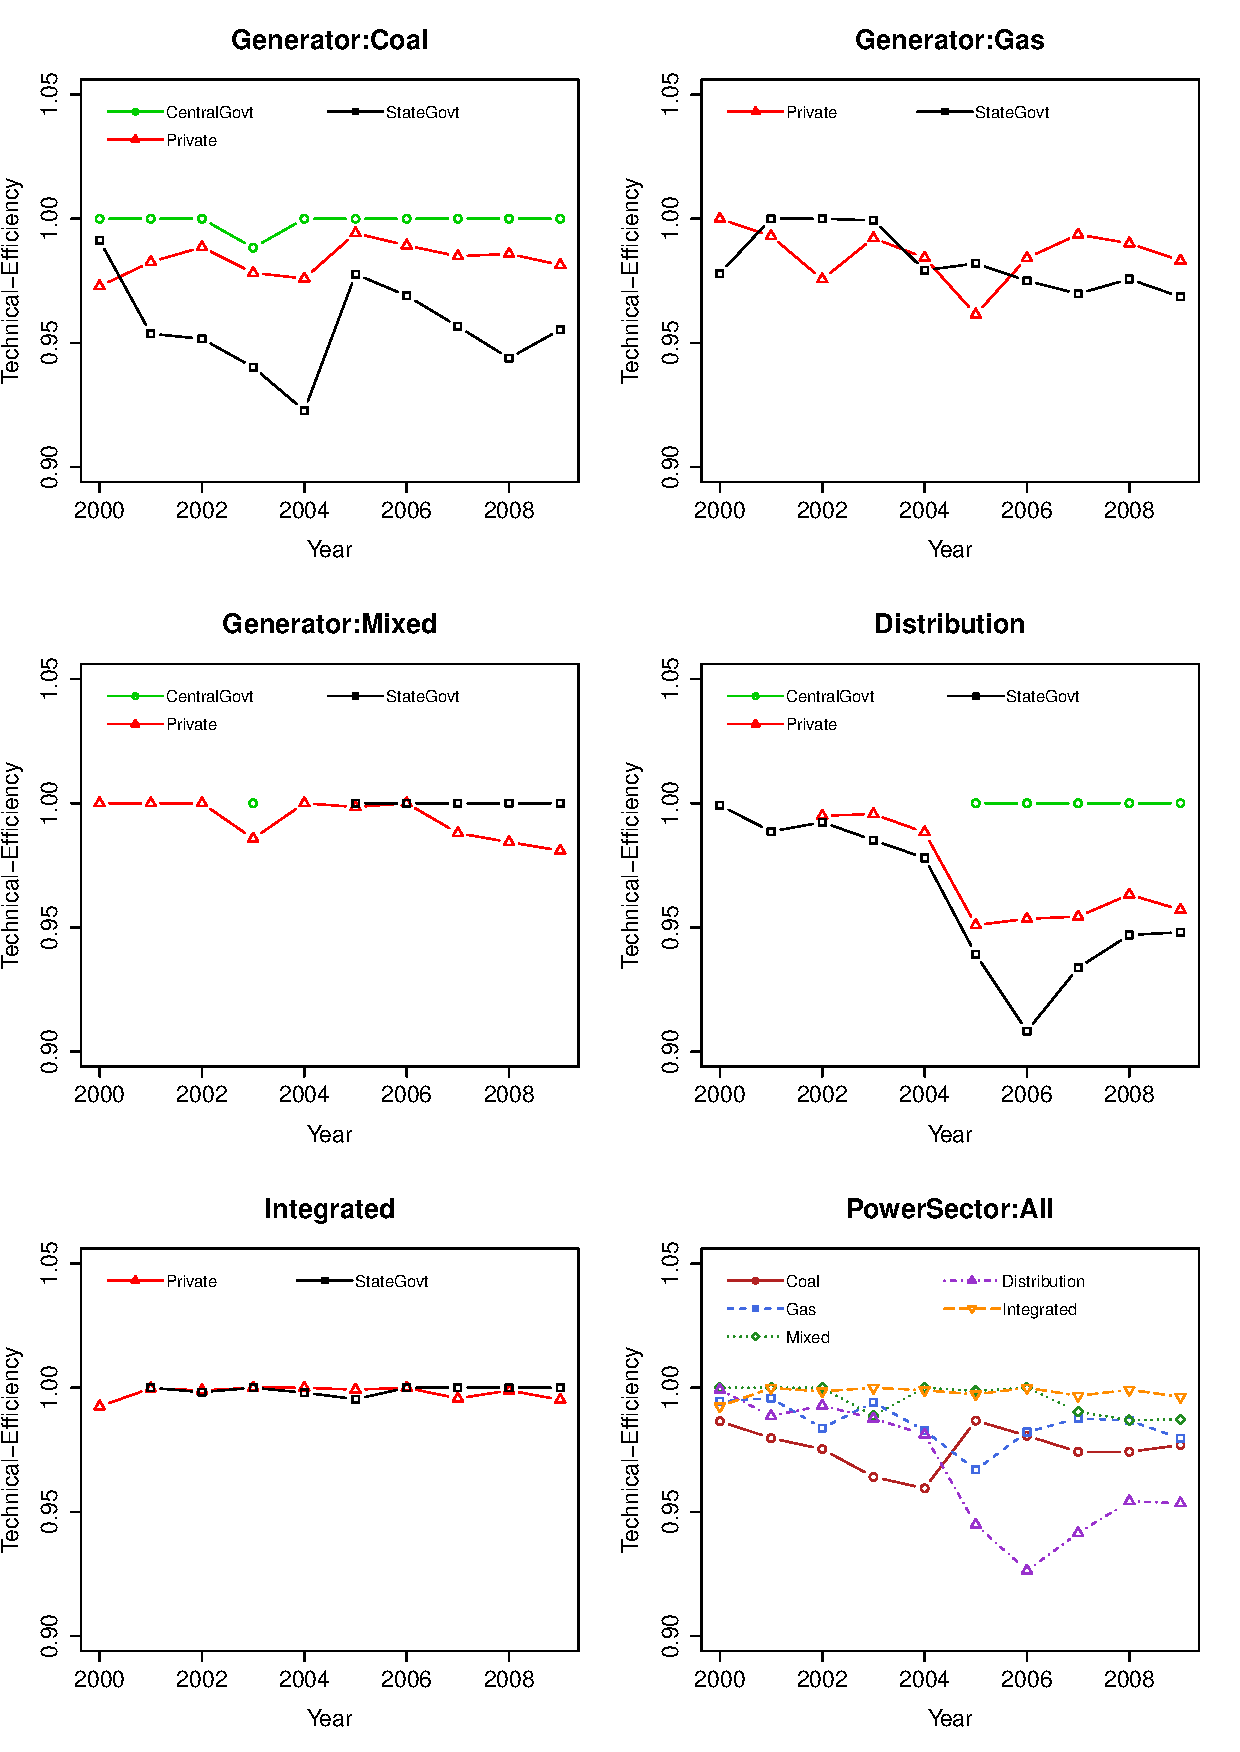
\includegraphics[width=1.00\textwidth]{chapter03/DEATimeTrend.pdf}
		\label{fig:DEATimeTrend}
\end{figure}

\begin{figure}[ht]
	\centering
	\caption{Power Sector DEA Efficiency Distribution}
		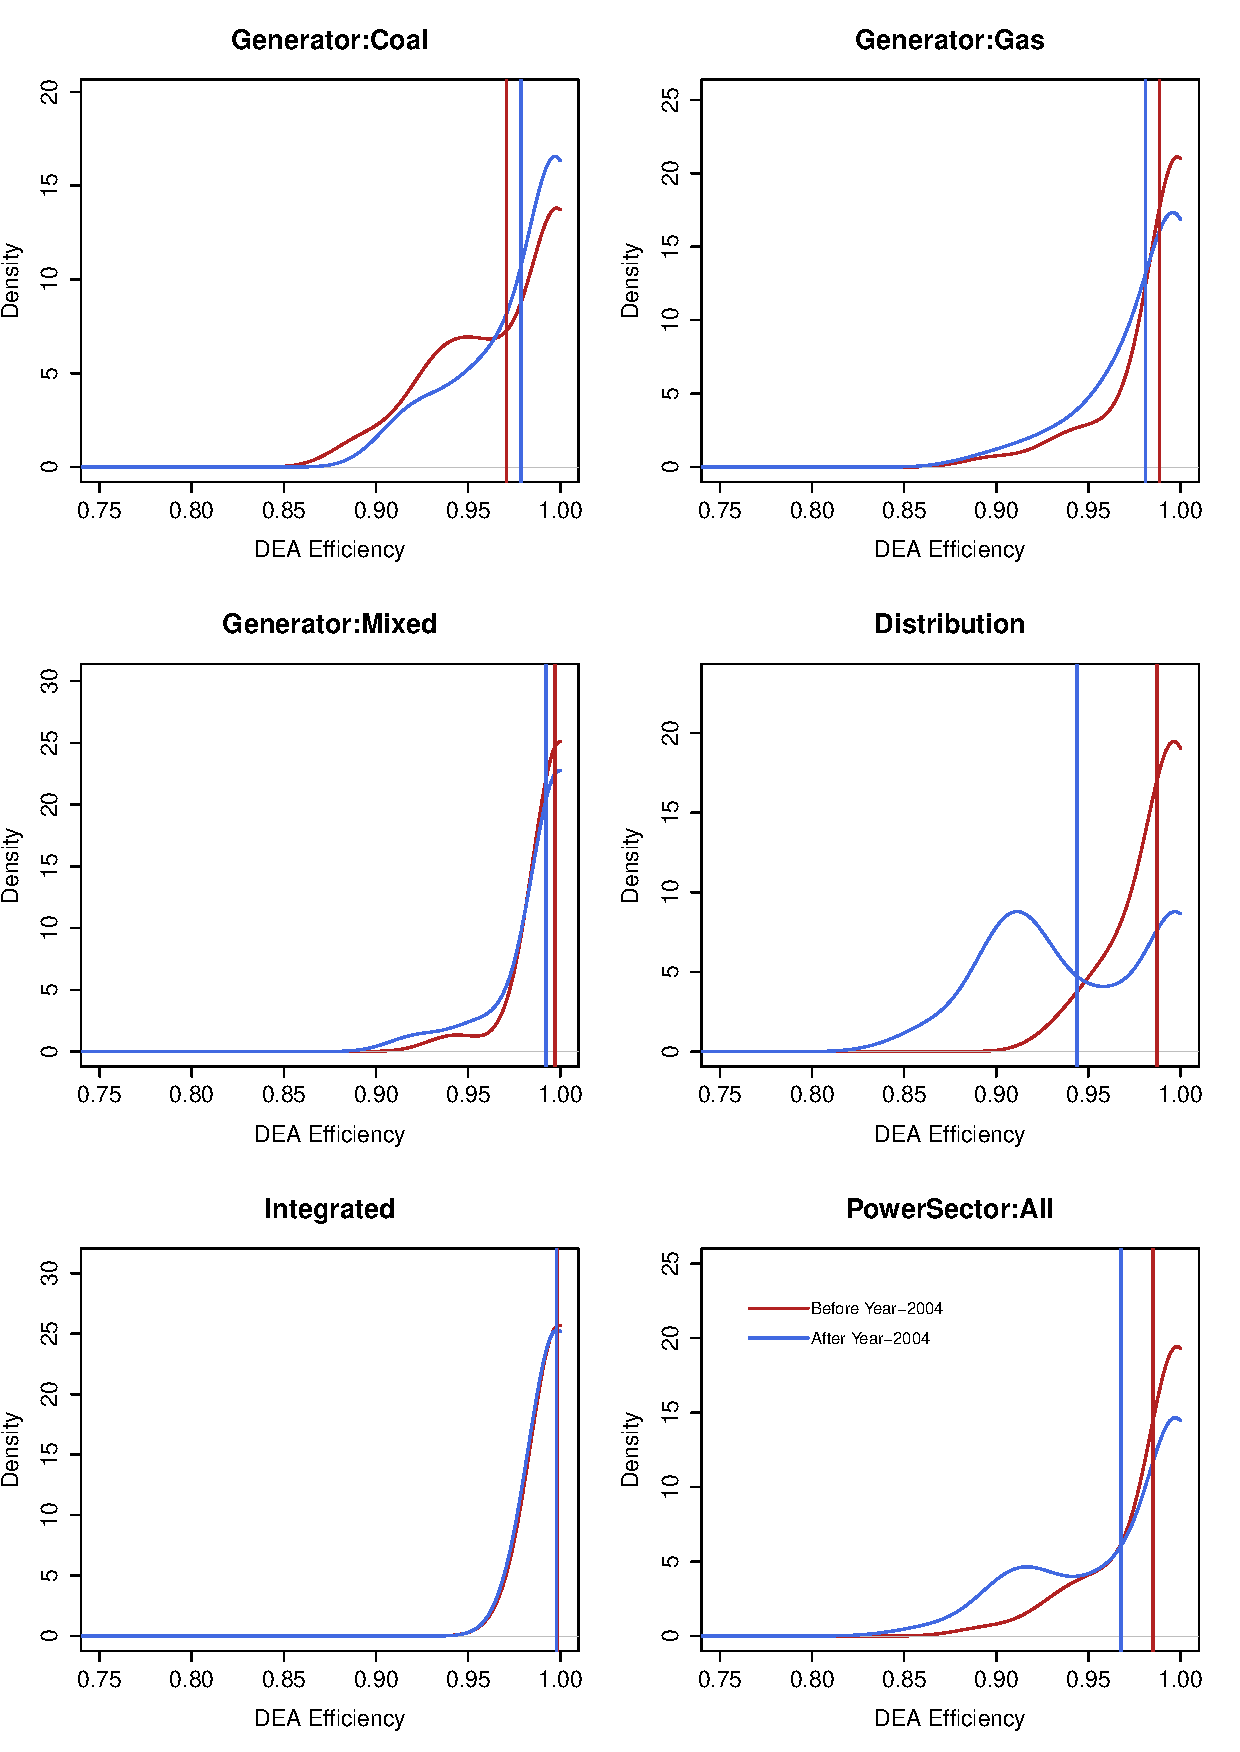
\includegraphics[width=1.00\textwidth]{chapter03/DEAEfficiency.pdf}
	\label{fig:DEAEfficiency}
\end{figure}

\begin{figure}[ht]
	\centering
	\caption{Power Sector TFP (Malmquist) Change Index}
		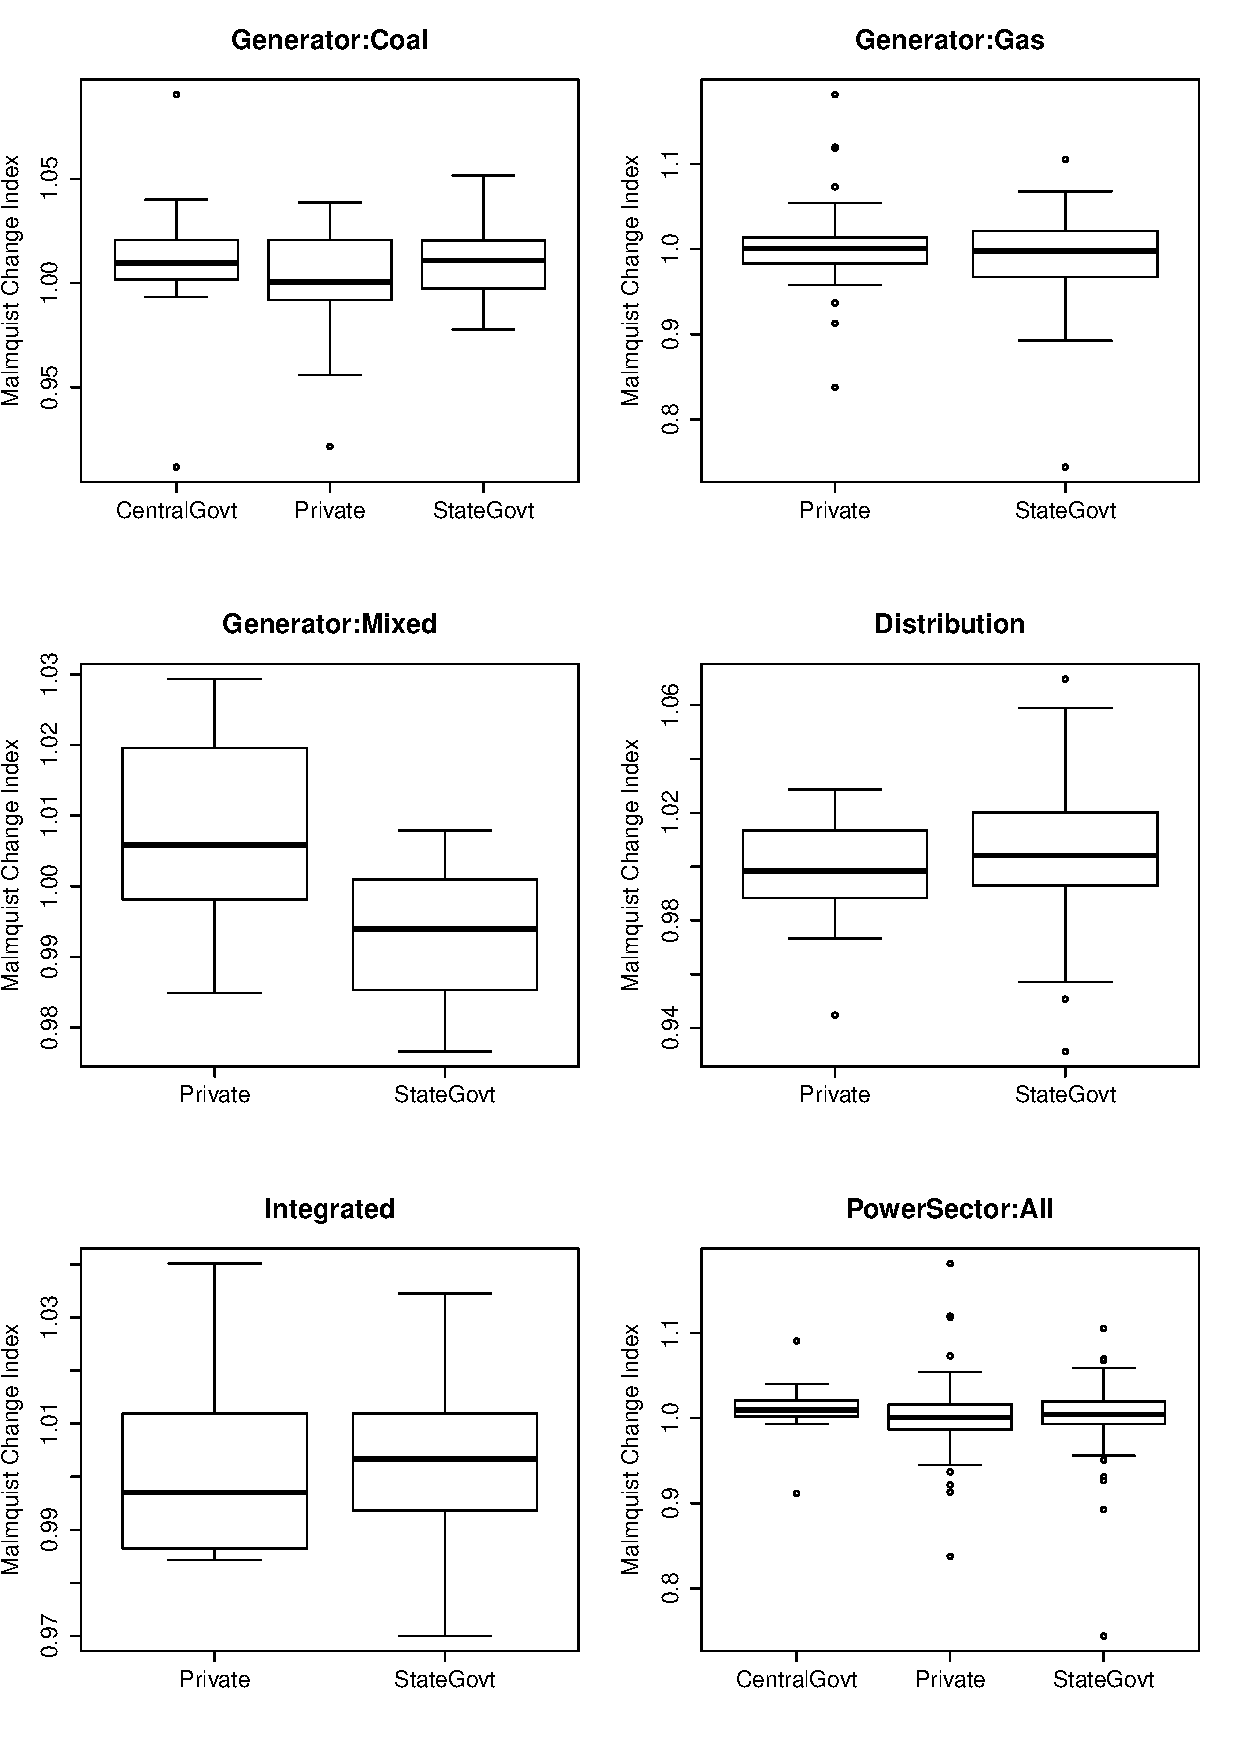
\includegraphics[width=1.00\textwidth]{chapter03/MalmIndex.pdf}	
	\label{fig:MalmIndex}
\end{figure}

\begin{figure}[ht]
	\centering
	\caption{Power Sector Pure Efficiency Change}
		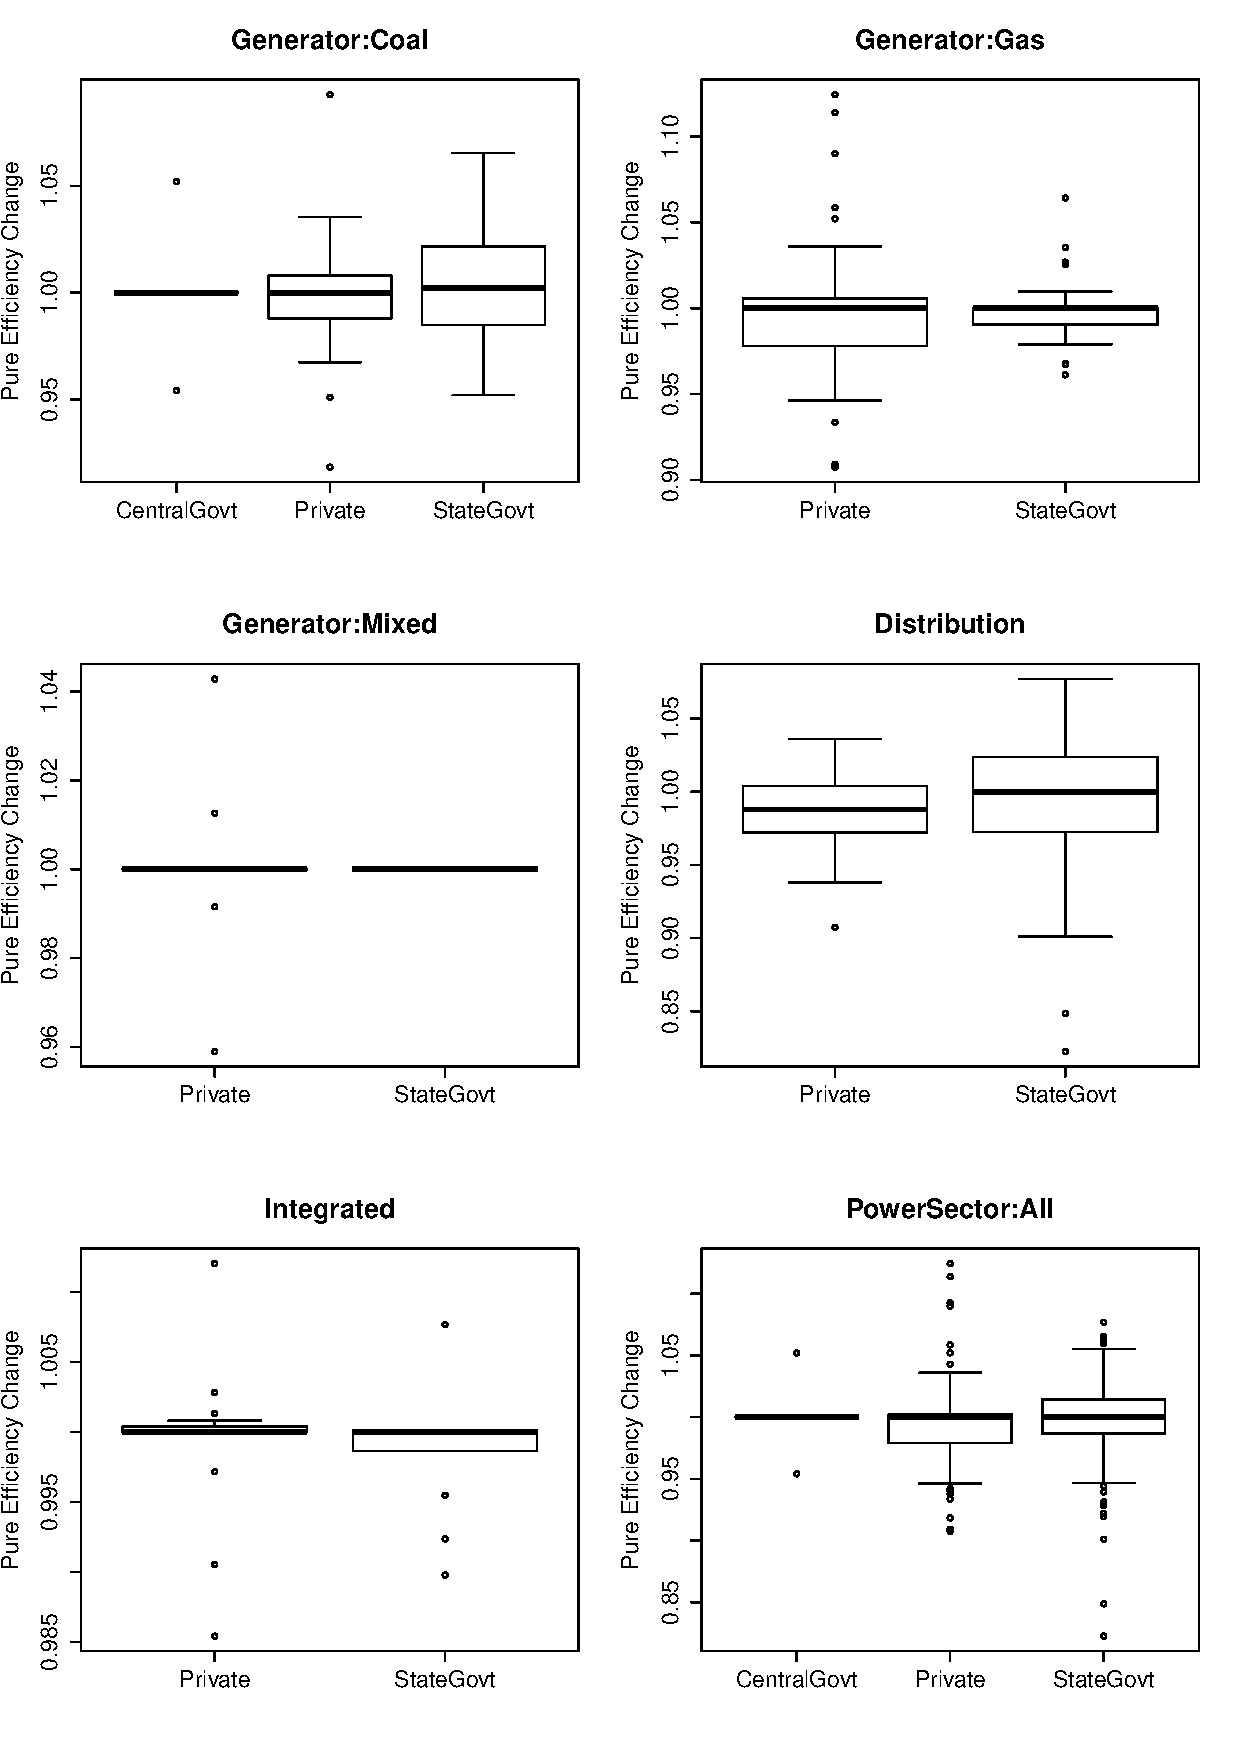
\includegraphics[width=1.00\textwidth]{chapter03/PureEffChange.pdf}
	\label{fig:PureEffChange}
\end{figure}

\begin{figure}[ht]
	\centering
	\caption{Power Sector Scale Change Effect}
		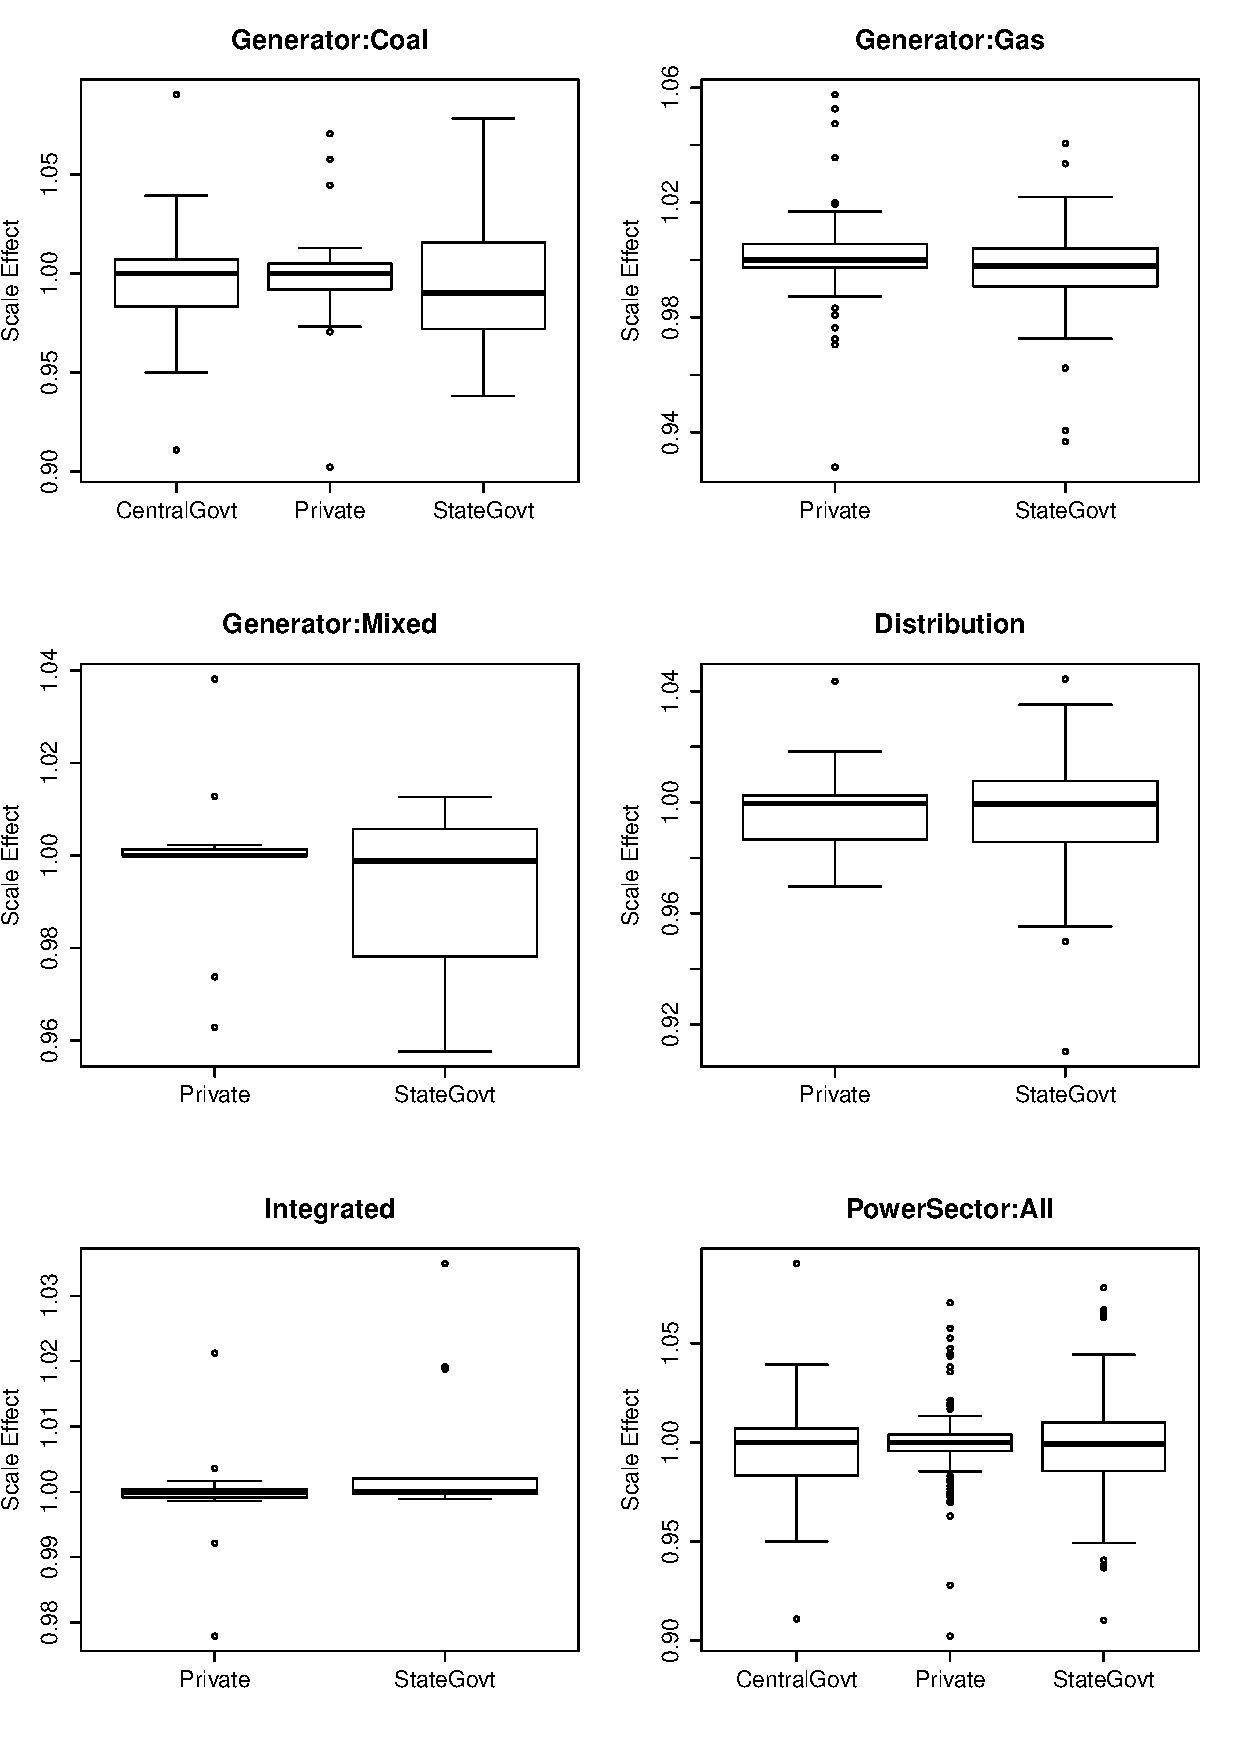
\includegraphics[width=1.00\textwidth]{chapter03/ScaleEffect.pdf}	
	\label{fig:ScaleEffect}
\end{figure}

\begin{figure}[ht]
	\centering
	\caption{Power Sector Pure Technology Change}
		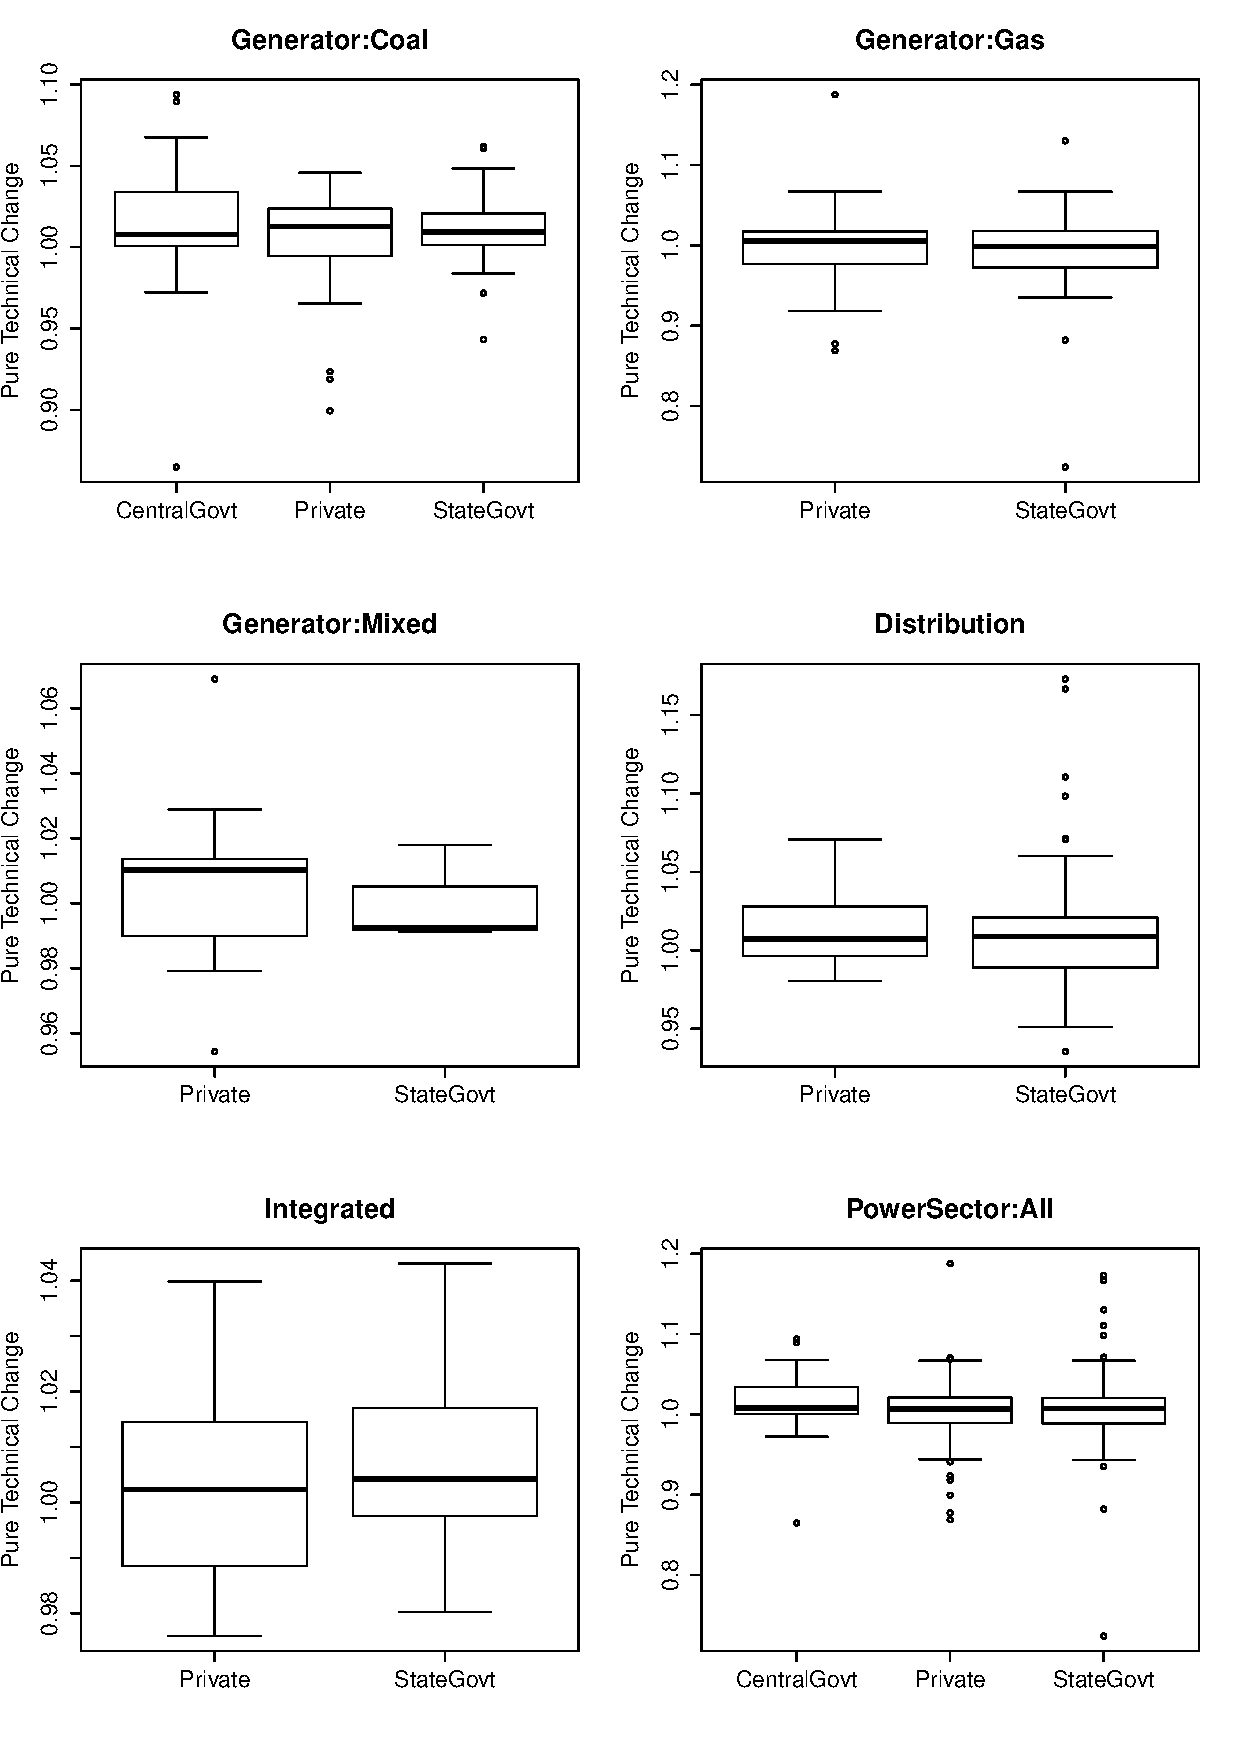
\includegraphics[width=1.00\textwidth]{chapter03/PureTechChange.pdf}
	\label{fig:PureTechChange}
\end{figure}

\begin{figure}[ht]
	\centering
	\caption{Power Sector Technology-Scale Change Effect}
		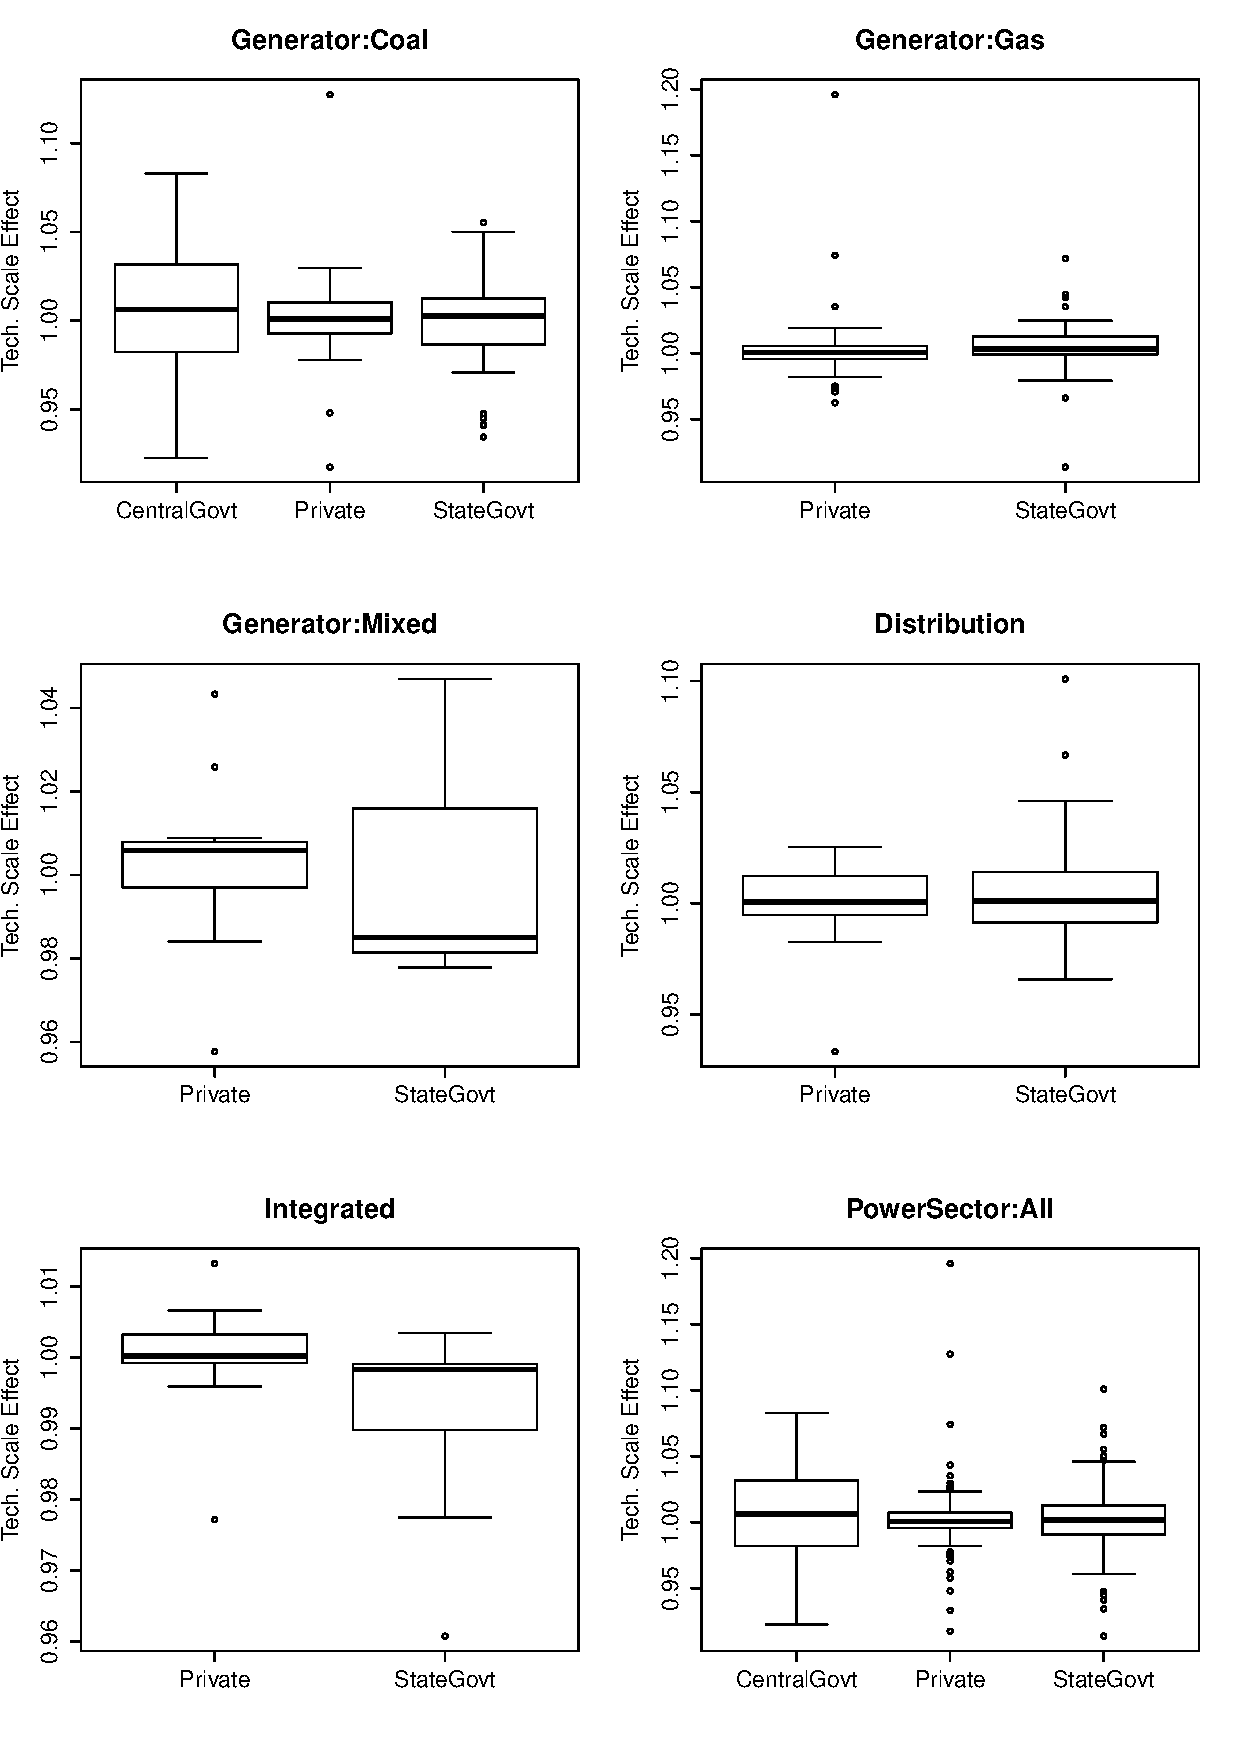
\includegraphics[width=1.00\textwidth]{chapter03/TechScale.pdf}
	\label{fig:TechScale}
\end{figure}


\bibliographystyle{apalike} 
\onehalfspacing
%\singlespacing
\bibliography{chap03refs}



\doublespacing
%\singlespacing
%\onehalfspacing
\appendix
\chapter{Within Transformed SFA Model}
\label{app:A}
%% Appendix A
\section{SFA Model Specification}
%\label{app:A}
\noindent The within transformed SFA model \citep{Wang2010} used in this paper is described here. Consider an SFA model with the following general specifications$:$
\begin{eqnarray}
y_{it} & = &\alpha_{i}+\mathbf{x}_{nit}\boldsymbol\beta+\mathbf{\epsilon}_{it},
\hspace{1em} i=1,\ldots,I,\hspace{1em}t=1,\ldots,T,\hspace{1em}n=1,\ldots,N
\label{eqn:ineff1}\\
\epsilon_{it} & = &v_{it} - u_{it},\\
v_{it} &\sim& N(0,\sigma_{v}^{2}),\\
u_{it} &=& h_{it}~.~\bar{u}_{i},\\
h_{it} &=& f(\mathbf{z}_{kit}\mathbf{\delta}),\hspace{1em}k=1,\ldots,K\\
\bar{u}_{i} &\sim& N^{+}(\mu,\sigma_{u}^{2}).\label{eqn:ineff6}
\end{eqnarray}
Here, $\mathbf{x}_{nit}$ is a vector of $N$ production factor variables (or explanatory variables in general) and $\alpha_{it}$ represents unobserved fixed effect corresponding to the $i^{th}$ firm. $v_{it}\sim N(0,\sigma_{v}^{2})$ is the noise component and $\bar{u}_{it}$ 
is the nonnegative stochastic technical inefficiency component. While $\bar{u}_{it}$ is defined as a truncated normal distribution (Eq.\ref{eqn:ineff6}), in our model we set $\mu=0$ and assume a half-normal distribution for the inefficiency component. The vector $\mathbf{z}_{kit}$ represents $K$ exogenous variables determining inefficiency. 

\section{Transformed Specification}
The \emph{within transformation} is obtained by subtracting the sample mean of each panel
from every individual observation in the panel. The transformation, by de-meaning, removes
time-invariant fixed effects from the model. The model specification (Eq.\ref{eqn:ineff1}-\ref{eqn:ineff6}) post transformation may be represented as$:$

\begin{eqnarray}
\tilde{y}_{i*} & = &\mathbf{\tilde{x}}_{ni*}\boldsymbol\beta+\mathbf{\tilde{\epsilon}}_{i*},
\label{eqn:tineff1}\\
\tilde{\epsilon}_{i*} & = &\tilde{v}_{i*} - \tilde{u}_{i*},\\
\tilde{v}_{i*} &\sim& \mathbf{N}(0,\Pi),\label{eqn:tineff3}\\
\tilde{u}_{i*} &=& \tilde{h}_{i*}~.~\bar{u}_{i},\\
\bar{u}_{i} &\sim& N^{+}(\mu,\sigma_{u}^{2}).\label{eqn:tineff5}
\end{eqnarray}

Here, we denote mean of individuals over the panel by $y_{i*} = (1/T)\Sigma^{T}_{t=1}y_{it}$, and the mean differenced value by $y_{it*}=y_{it}-y_{i*}$. The full panel as a vector stack is represented as

$\tilde{y}_{i*} = (y_{i1},y_{i2},\ldots,y_{iT})'$. The variance-covariance matrix of $\tilde{v}_{i*}$ (Eqn. \ref{eqn:tineff3}) is
\begin{equation}
\label{eqn:mat}
\Pi = \begin{bmatrix}
\sigma^{2}_{v}(1-1/T) & \sigma^{2}_{v}(-1/T) &\cdots& \sigma^{2}_{v}(-1/T) \\
\sigma^{2}_{v}(-1/T) & \sigma^{2}_{v}(1-1/T) &\cdots& \sigma^{2}_{v}(-1/T) \\
\vdots & \vdots & \ddots & \vdots \\
\sigma^{2}_{v}(-1/T) & \sigma^{2}_{v}(-1/T) &\cdots& \sigma^{2}_{v}(1-1/T) \\
 \end{bmatrix} 
\end{equation}
\section{Log-Likelihood Function}
For the model described above, \cite{Wang2010} derives the marginal log-likelihood function of the $i^{th}$ panel as follows, 
\begin{equation}
\label{eqn:loglik}
\begin{split}
ln~L_{i} &= -\frac{1}{2}(T-1)ln(2\pi)-\frac{1}{2}(T-1)ln(\sigma^{2}_{v})-\frac{1}{2}\tilde{\epsilon}_{i*}'\Pi^{-}\tilde{\epsilon}_{i*}+\frac{1}{2}\left(\frac{\mu^{2}_{1}}{\sigma^{2}_{1}}-\frac{\mu^{2}}{\sigma^{2}}\right)\\
& +ln\left(\sigma_{1}\Phi\left(\frac{\mu_{1}}{\sigma_{1}}\right)\right) -ln\left(\sigma_{u}\Phi\left(\frac{\mu}{\sigma_{u}}\right)\right),
\end{split}
\end{equation}
where $\Pi^{-}$ is the generalized inverse of $\Pi$, $\phi$ the normal density function, $\Phi$ the cumulative density function and, 
\begin{equation}
\mu_{1}=\frac{\mu/\sigma_{u}^{2}-\tilde{\epsilon}_{i*}'\Pi^{-}\tilde{h}_{i*}}{\tilde{h}_{i*}'\Pi^{-}\tilde{h}_{i*} + 1/\sigma^{2}_{u}},
\end{equation}
\begin{equation}
\sigma_{1}^2=\frac{1}{\tilde{h}_{i*}'\Pi^{-}\tilde{h}_{i*} + 1/\sigma^{2}_{u}},
\end{equation}
\begin{equation}
\tilde{\epsilon}_{i*}=\tilde{y}_{i*}-\mathbf{\tilde{x}}_{i*}\beta
\end{equation}
The log likelihood function of the model $L$ is obtained by summing the marginal likelihood over $i=1,\ldots,I$
\begin{equation}
L=\Sigma^{I}_{i=1}L_{i}
\end{equation} 
\section{Inefficiency and Fixed-Effect Estimation}
The inefficiency index of observation/firm, $i$, during period, $t$, can be estimated as the expection of $u_{it}$ conditional on the model residue, $\tilde{\epsilon}_{i*}~:$
\begin{equation}
\label{eqn:inefind}
E\left(u_{it}|\tilde{\epsilon}_{i*}\right)=h_{it}\left[\mu_{1}+\frac{\phi\left(\frac{\mu_{1}}{\sigma_1}\right)\sigma_{1}}{\Phi\left(\frac{\mu_{1}}{\sigma_1}\right)}\right]
\end{equation}
The fixed-effects, $\alpha_{i}$'s, can be recovered from the estimates of parameters obtained, 
\begin{equation}
\label{eq:fixeff}
\hat{\alpha}_{i}=y_{i*}-\boldsymbol{x}_{i*}\boldsymbol{\hat{\beta}}+\hat{\mu}_{2}\hat{h}_{i*}+\hat{\sigma}_{2}\hat{h}_{i*}\frac{\phi\left(\frac{\hat{\mu}_{2}}{\hat{\sigma}_2}\right)}{\Phi\left(\frac{\hat{\mu}_{2}}{\hat{\sigma}_2}\right),}
\end{equation}
where
\begin{equation}
\hat{\mu}_{2}=\frac{\hat{\mu}\hat{\sigma}^{-2}_{u}-\hat{\sigma}^{-2T}_{v}\sum_{t}\hat{\epsilon}_{it}\hat{h}_{it}}{\hat{\sigma}^{-2T}_{v}\sum_{t}\hat{h}_{it}^{2}+\hat{\sigma}^{-2}_{u}}
\end{equation}
\begin{equation}
\hat{\sigma}^{2}_{2}=\frac{\hat{\sigma}^{2T}_{v}}{\sum_{t}\hat{h}_{it}^{2}+\hat{\sigma}^{2T}_{v}\hat{\sigma}^{-2}_{u}}
\end{equation}
\section{R-Code}
A routine, in the R-statistical language, is written to estimate the maximum likelihood function (Eq. \ref{eqn:loglik}). Additional routines computes inefficiency indices following Eq. \ref{eqn:inefind} and the firm fixed-effects following Eq. \ref{eq:fixeff}. The R-code is tested with STATA procedure and test data obtained from Hun-Jen Wang, as described in detail in \cite{Wang2010}. In addition Monte Carlo simulations are done to test the R-routine. The complete R-code is available freely from the authors on request. The function for MLE estimation of parameters is described in code listing \ref{Rcode1}. R functions for efficiency and firm fixed effects estimation is listed in \ref{Rcode2} and the function for numerical computation of the Hessian matrix of the estimated parameters for computing standard errors is listed in \ref{Rcode3}.
\vskip 1cm

\begin{lstlisting}[label=Rcode1, caption=R-Code for Maximum Likelihood Function]   
##########################################################
# Maximum Likelihood Estimation 
# Within Transformed SFA Models
# Version: v1.0
# Author : Anish Sugathan
# E-mail : anish.iimb@gmail.com 
########################################################## 
#The function sfa.within returns model parameters estimated
#using the maximum-likelihood estimation technique.
#Variable Definitions:
#theta   		: vector of parameters to be estimated
#data    		: R data.frame for the panel data 
#out.var 		: the variable name of output variable
#in.var  		: vector of input variable names
#z.var   		: vector of ineff. explanatory variable names
#id.var  		: variable name identifying individuals
#t.var	 		: variable name identifying panel time
#limitLH 		: len(theta)X2 matrix of parameter bounds
#optMethod	: optimization method to be used
#optControl	: list of optimization control parameters
#halfnormal	: (logical) TRUE or FALSE     
sfa.within<-function(theta,data, out.var, in.var, z.var, id.var, t.var,limitLH, optMethod,optControl,halfnorm=FALSE){
  
  #Compute total time periods for each firm
  compNames<-unique(data[,id.var])
  for(i in 1:length(compNames)){
    years<-sort(data[data[,id.var]==compNames[i],t.var])
    data$TP[data[,id.var]==compNames[i]]<-length(years)  
    data$CompCode[data[,id.var]==compNames[i]]<-i
  }  
  data<-data[data$TP>=2,]
  data<-data[order(data[,id.var],data[,t.var]),]
  
  #Compute delta and h_it
  delta<-theta[(3+NCOL(data[,in.var])+1):(3+NCOL(data[,in.var])+NCOL(data[,z.var]))]
  data$h_it<-exp(as.matrix(data[,z.var]) %*% delta)
  
  #Compute the mean subtracted values  
  for(i in 1:length(compNames)){    
    for(k in c(out.var,in.var,'h_it')){
      data[data[,id.var]==compNames[i],paste('W_',k,sep='')]<-data[data[,id.var]==compNames[i],k]-mean(data[data[,id.var]==compNames[i],k])
    }    
  }
  if(is.numeric(data[,t.var])){
    select.vars<-c(t.var,'CompCode',out.var,in.var,z.var,'h_it','W_h_it','TP',paste('W_',out.var,sep=''),paste('W_',in.var,sep=''))
  }else{
    stop(paste(t.var,': is not numeric. Only numeric t.vars allowed'))
  }
  
  datam<-as.matrix(data[,select.vars])
  
  CD<-datam[,'CompCode']
  Y<-datam[,paste('W_',out.var,sep='')]  
  X<-datam[,paste('W_',in.var,sep='')]
  Z<-datam[,z.var]
  TP<-datam[,'TP']
  H_it<-datam[,'W_h_it']
  S_H_it<-datam[,'h_it']
    
  #The Log Liklihood function (Wang and Ho,2010: p.288 Eq.13)
  logLikFun<-function(theta,Y,X,Z,TP,CD){    
    # Get parameters parsed from theta
    #mu <- 0 # to get the Ui* to follow a half normal distribution
    if(halfnorm==FALSE){
      mu <-theta[1]  
    }else{
      mu <- 0
    }    
    sigma_u<-exp(0.5*theta[2])#theta[2]#
    sigma_v<-exp(0.5*theta[3])#theta[3]#
    beta<-theta[4:(3+NCOL(X))]
    delta<-theta[(3+NCOL(X)+1):(3+NCOL(X)+NCOL(Z))]
    
    #function for repeated computation of liklihood for each panel
    getLogLik<-function(tp,mu,sigma_v,sigma_u,y,x,z,w_h_it){      
      epsi<- y - x %*% beta    
      
      PI<-(sigma_v^2)*(diag(tp)-rep(1/tp,tp))
      PIi<-ginv(PI)      
      
      Aa<-t(epsi) %*% PIi %*% w_h_it
      Bb<-t(w_h_it) %*% PIi %*% w_h_it + 1/sigma_u^2
      Cc<-t(epsi) %*% PIi %*% epsi
      
      mu_star<-(mu/sigma_u^2 - Aa)/Bb
      sigma2_star<-1/Bb
      sigma_star<-sqrt(sigma2_star)      
      
      Dd<-((mu_star^2/sigma2_star)-(mu^2/sigma_u^2))
      Ee<-log(sigma_star*pnorm(mu_star/sigma_star))
      Ff<-log(sigma_u*pnorm(mu/sigma_u))
      
      logLikVal<- -0.5*(tp-1)*log(2*pi)-0.5*(tp-1)*log(sigma_v^2)-0.5*Cc+0.5*Dd+Ee-Ff        
      return(logLikVal)       
    }# end of function getLogLik
       
    logLikSum<-0
    if(sigma_u >=0 & sigma_v >=0){
      #if(ifelse(limitLH==NULL,sigma_u >=0 & sigma_v >=0,!sum(theta<limitLH[,1]) & !sum(theta>limitLH[,2]))){
      codes<-unique(CD)      
      logLikSum<-0        
      for(cd in codes){
        y<-Y[CD==cd]
        x<-X[CD==cd,]
        if(NCOL(Z)>=2){
          z<-Z[CD==cd,]
        }else{
          z<-Z[CD==cd]
        }
        tp<-TP[CD==cd][1]
        w_h_it<-exp(z %*% delta)
        w_h_it<-w_h_it-mean(w_h_it)
        logLikVal<- getLogLik(tp=tp,mu=mu,sigma_v=sigma_v,sigma_u=sigma_u,y=y,x=x,z=z,w_h_it=w_h_it)         
        logLikSum<-logLikSum + logLikVal      
      }      
      if(optMethod=='BFGS' 
         |optMethod=='nloptr'
         |optMethod=='bobyqa'
         |optMethod=='DEoptim'){
        return(ifelse(is.na(logLikSum),1e20,-1*logLikSum))#for DEoptim        
      }else{        
        return(sum(logLikSum))
      }      
      }else{
        if(!(optMethod=='DEoptim'))
        {
          return(NA)
        }else{
          return(1e20)
        }
      }         
    }
    #end of function LogLik
  print('Data Processed..Optimization Call Start.')
  switch(optMethod,
         'genoud'={
            opt <- genoud(logLikFun, nvars = length(theta),max=TRUE
                         ,pop.size=5000,starting.values=theta
                         ,default.domains=10
                         ,hessian=FALSE,optim.method='BFGS'
                         ,max.generations=10                         
                         ,Y=Y,X=X,Z=Z,TP=TP,CD=CD)         
           opt<-rename(opt,c(value='fval'))                    
           },
         'DEoptim'={
           lb=rep(-5,length(theta)) 
           ub=rep(+5,length(theta))
           theta[1]<-0
           maxit<-100
           opt<- DEoptim(fn=logLikFun,lower=lb,upper=ub
                         ,DEoptim.control(NP=20*length(theta)
                                          ,F=1,itermax=maxit
                                          ,p=0.2,strategy=6 ),Y=Y,X=X,Z=Z,TP=TP,CD=CD)
         },
         'nloptr'={
           lb=c(0,rep(-10,length(theta)-1))
           ub=c(0,rep(+10,length(theta)-1))
           theta[1]<-0
           options<-list(algorithm="NLOPT_GN_CRS2_LM"
                         ,check_derivatives = FALSE
                         ,check_derivatives_print = "none"
                         ,print_level=2
                         ,maxeval=1000                         
                         )
           opt <- nloptr(x0=theta
                         ,eval_f=logLikFun
                         ,eval_grad_f=NULL
                         ,eval_g_ineq=NULL
                         ,eval_jac_g_ineq=NULL
                         ,eval_g_eq=NULL
                         ,eval_jac_g_eq=NULL
                         ,lb=lb
                         ,ub=ub
                         ,opts<-options
                         ,Y=Y,X=X,Z=Z,TP=TP,CD=CD)
           },         
           'bobyqa'={
             lb=c(0,rep(-10,length(theta)-1)) 
             ub=c(1e-1,rep(+10,length(theta)-1))
             theta[1]<-0
             ctrl=list(npt=length(theta)*2+1
                       ,rhobeg=1e-1
                       ,rhoend=1e-6
                       ,iprint=2
                       ,maxfun=optControl$maxit
                       ,boundary.enforcement=1)
             opt<-bobyqa(theta,logLikFun,lower=lb,upper=ub
                         ,control=ctrl
                         ,Y=Y,X=X,Z=Z,TP=TP,CD=CD)
           },
           'defalut'={
             print('Optimization Done!')
           }
  )
  return(list(optim=opt))          
}
#end of main function sfa.within

\end{lstlisting}


\begin{lstlisting}[label=Rcode2, caption=R-Code for Efficiency and Fixed Effects Estimation]   
##########################################################
# Efficiency and Fixed Effects Estimation of
# Within Transformed SFA Models
# Version: v1.0
# Author : Anish Sugathan
# E-mail : anish.iimb@gmail.com 
########################################################## 
#The function sfa.within.eff returns estimated
#Inefficiency scores and firm fixed effects
#Variable Definitions:
#theta   		: vector of parameters to be estimated
#data    		: R data.frame for the panel data 
#out.var 		: the variable name of output variable
#in.var  		: vector of input variable names
#z.var   		: vector of ineff. explanatory variable names
#id.var  		: variable name identifying individuals
#t.var	 		: variable name identifying panel time
#limitLH 		: len(theta)X2 matrix of parameter bounds
#optMethod	: optimization method to be used
#optControl	: list of optimization control parameters
#halfnormal	: (logical) TRUE or FALSE     

sfa.within.eff<-function(theta,data, out.var, in.var, z.var, id.var, t.var, halfnorm=TRUE){
  
  #Compute total time periods for each firm
  compNames<-unique(data[,id.var])
  for(i in 1:length(compNames)){
    years<-sort(data[data[,id.var]==compNames[i],t.var])
    data$TP[data[,id.var]==compNames[i]]<-length(years)  
    data$CompCode[data[,id.var]==compNames[i]]<-i
  }  
  data<-data[data$TP>=2,]
  data<-data[order(data[,id.var],data[,t.var]),]
  
  #Compute delta and h_it
  delta<-theta[(3+NCOL(data[,in.var])+1):(3+NCOL(data[,in.var])+NCOL(data[,z.var]))]
  data$h_it<-exp(as.matrix(data[,z.var]) %*% delta)  
  
  #Compute the mean subtracted values  
  for(i in 1:length(compNames)){    
    for(k in c(out.var,in.var,'h_it')){
      data[data[,id.var]==compNames[i],paste('W_',k,sep='')]<-data[data[,id.var]==compNames[i],k]-mean(data[data[,id.var]==compNames[i],k])
    }    
  }
  if(is.numeric(data[,t.var])){
    select.vars<-c(t.var,'CompCode',out.var,in.var,z.var,'h_it','W_h_it','TP',paste('W_',out.var,sep=''),paste('W_',in.var,sep=''))
  }else{
    stop(paste(t.var,': is not numeric. Only numeric t.vars allowed'))
  }
  
  datam<-as.matrix(data[,select.vars])
  #datam<-as.matrix(data[,select.vars])
  #datam<-datam[datam[,'FirstYear']==0,]
  
  CD<-datam[,'CompCode']
  Y<-datam[,paste('W_',out.var,sep='')]  
  X<-datam[,paste('W_',in.var,sep='')]
  Z<-datam[,z.var]
  TP<-datam[,'TP']
  H_it<-datam[,'W_h_it']
  S_H_it<-datam[,'h_it']  

    getEfficiency<-function(theta,Y,X,Z,TP,FY,CD){    
    ### function for repeated computation parameters for each panel
    getPar<-function(tp,mu,sigma_v,sigma_u,y,x,z,w_h_it,s_h_it){      
      epsi<- y - x %*% beta    
      
      PI<-(sigma_v^2)*(diag(tp)-rep(1/tp,tp))
      PIi<-ginv(PI)      
      
      Aa<-t(epsi) %*% PIi %*% w_h_it
      Bb<-t(w_h_it) %*% PIi %*% w_h_it + 1/sigma_u^2
      Cc<-t(epsi) %*% PIi %*% epsi
      
      mu_star<-(mu/sigma_u^2 - Aa)/Bb
      sigma2_star<-1/Bb
      sigma_star<-sqrt(sigma2_star)      
      
      ## Recover Individual Fixed Effects
      Dd <- mu/sigma_u^2 - (1/sigma_v^(2*(tp)))*sum(epsi*s_h_it) 
      Ee <- (1/sigma_v^(2*(tp)))*sum(s_h_it^2) + 1/sigma_u^2
      Ff <- sum(s_h_it^2) + sigma_v^(2*(tp))/sigma_u^2
      mu_starry<-Dd/Ee
      sigma2_starry<-sigma_v^(2*(tp))/Ff
      sigma_starry<-sqrt(sigma2_starry)
      
      y_dot <- mean(y)
      x_dot <- apply(x,2,mean)
      h_dot <- mean(s_h_it)
      
      # a small empsilon = 1e-20 is added to avoid NANs
      Gg<-(dnorm(mu_starry/sigma_starry)+1e-20)/(pnorm(mu_starry/sigma_starry)+1e-20)
      
      alph <- y_dot - x_dot %*% beta + mu_starry*h_dot + sigma_starry*h_dot*(Gg) 
      
      return(cbind(mu_star,sigma_star,mu_starry,sigma_starry,alph))       
    }# end of function getPar
    
    # Get parameters parsed from theta    
    if(halfnorm==FALSE){
      mu <-theta[1] 
    }else{
      mu <- 0
    }    
    sigma_u<-exp(0.5*theta[2])#theta[2]#
    sigma_v<-exp(0.5*theta[3])#theta[3]#
    beta<-theta[4:(3+NCOL(X))]
    delta<-theta[(3+NCOL(X)+1):(3+NCOL(X)+NCOL(Z))]
    
    codes<-unique(CD)
    CD_h_it<-cbind(CD,0)
    CDPar<-matrix(nrow=length(codes),ncol=6)
    i<-1
    for(cd in codes){
      y<-Y[CD==cd]
      x<-X[CD==cd,]
      if(NCOL(Z)>=2){
        z<-Z[CD==cd,]
      }else{
        z<-Z[CD==cd]
      }
      tp<-TP[CD==cd][1]
      #w_h_it<-H_it[CD==cd]
      #s_h_it<-S_H_it[CD==cd]
      s_h_it<-exp(z %*% delta)
      w_h_it<-s_h_it-mean(s_h_it)
      CD_h_it[CD==cd,2]<-s_h_it###<check this      
      
      #getPar(tp,mu,sigma_v,sigma_u,y,x,z,w_h_it,s_h_it)
      
      CDPar[i,1]<-cd
      CDPar[i,2]<-getPar(tp,mu,sigma_v,sigma_u,y,x,z,w_h_it,s_h_it)[1]#mu_star
      CDPar[i,3]<-getPar(tp,mu,sigma_v,sigma_u,y,x,z,w_h_it,s_h_it)[2]#sigma_star
      CDPar[i,4]<-getPar(tp,mu,sigma_v,sigma_u,y,x,z,w_h_it,s_h_it)[3]#mu_starry
      CDPar[i,5]<-getPar(tp,mu,sigma_v,sigma_u,y,x,z,w_h_it,s_h_it)[4]#sigma_starry
      CDPar[i,6]<-getPar(tp,mu,sigma_v,sigma_u,y,x,z,w_h_it,s_h_it)[5]#alph
      i<-i+1
    }
    CD_h_it<-cbind(CD_h_it,NA,NA,NA,NA,NA)
    for(cd in codes){
      CD_h_it[CD_h_it[,1]==cd,3]<-CDPar[CDPar[,1]==cd,2]#mu_star
      CD_h_it[CD_h_it[,1]==cd,4]<-CDPar[CDPar[,1]==cd,3]#sigma_star
      CD_h_it[CD_h_it[,1]==cd,5]<-CDPar[CDPar[,1]==cd,4]#mu_starry
      CD_h_it[CD_h_it[,1]==cd,6]<-CDPar[CDPar[,1]==cd,5]#sigma_starry
      CD_h_it[CD_h_it[,1]==cd,7]<-CDPar[CDPar[,1]==cd,6]#alph
    }
    InEff<-CD_h_it[,2]*(CD_h_it[,3] + (dnorm(CD_h_it[,3]/CD_h_it[,4])*CD_h_it[,4])/pnorm(CD_h_it[,3]/CD_h_it[,4]))
    TEff<-exp(-InEff)
    CD_h_it<-cbind(CD_h_it,InEff,TEff)      
    return(CD_h_it)    
  }# end of getEfficiency   
  
Eff<-getEfficiency(theta,Y,X,Z,TP,FY,CD) 
datam<-cbind(datam,Eff[,-1])
  dimnames(datam)[2]<-list(c(select.vars,"h_it","mu_s","sig_s","mu_ss","sig_ss","alph","InEff_u","TEff"))
  dataf<-merge(data[,c('Year','CompanyName','CompCode')],data.frame(datam),by=c('Year','CompCode'))
  return(dataf)  
}
\end{lstlisting}




\begin{lstlisting}[label=Rcode3, caption=R-Code for Numerical Estimation of Hessian Matrix]   
##########################################################
# Numerical Hessian Matrix for Parameter Estimates of
# Within Transformed SFA Models
# Version: v1.0
# Author : Anish Sugathan
# E-mail : anish.iimb@gmail.com 
########################################################## 
#The function sfa.within.hessian returns estimated
#numerical hessian for standard error computation
#Variable Definitions:
#theta   		: vector of parameters to be estimated
#data    		: R data.frame for the panel data 
#out.var 		: the variable name of output variable
#in.var  		: vector of input variable names
#z.var   		: vector of ineff. explanatory variable names
#id.var  		: variable name identifying individuals
#t.var	 		: variable name identifying panel time
#limitLH 		: len(theta)X2 matrix of parameter bounds
#optMethod	: optimization method to be used
#optControl	: list of optimization control parameters
#halfnormal	: (logical) TRUE or FALSE     

sfa.within.hessian<-function(theta,data, out.var, in.var, z.var, id.var, t.var, halfnorm=TRUE,onlyLogLik){
  
  #theta such that (mu, sigma_u, sigma_v, beta, delta)
  #theta<-c(0,1,1,rep(0,length(in.var)+length(z.var)))
  print('Preparing Data...')
  ## Prepare the data object for fast iterations
  
  #Compute total time periods for each firm
  compNames<-unique(data[,id.var])
  for(i in 1:length(compNames)){
    years<-sort(data[data[,id.var]==compNames[i],t.var])
    data$TP[data[,id.var]==compNames[i]]<-length(years)  
    data$CompCode[data[,id.var]==compNames[i]]<-i
  }  
  
  data<-data[data$TP>=2,]
  data<-data[order(data[,id.var],data[,t.var]),]
  
  #Compute delta and h_it
  delta<-theta[(3+NCOL(data[,in.var])+1):(3+NCOL(data[,in.var])+NCOL(data[,z.var]))]
  data$h_it<-exp(as.matrix(data[,z.var]) %*% delta)  
  
  #Compute the mean subtracted values  
  for(i in 1:length(compNames)){    
    for(k in c(out.var,in.var,'h_it')){
      #print(k)
      data[data[,id.var]==compNames[i],paste('W_',k,sep='')]<-data[data[,id.var]==compNames[i],k]-mean(data[data[,id.var]==compNames[i],k])
    }    
  }
  if(is.numeric(data[,t.var])){
    select.vars<-c(t.var,'CompCode',out.var,in.var,z.var,'h_it','W_h_it','TP',paste('W_',out.var,sep=''),paste('W_',in.var,sep=''))
  }else{
    stop(paste(t.var,': is not numeric. Only numeric t.vars allowed'))
  }
  
  datam<-as.matrix(data[,select.vars])
  #datam<-as.matrix(data[,select.vars])
  #datam<-datam[datam[,'FirstYear']==0,]
  
  CD<-datam[,'CompCode']
  Y<-datam[,paste('W_',out.var,sep='')]  
  X<-datam[,paste('W_',in.var,sep='')]
  Z<-datam[,z.var]
  TP<-datam[,'TP']
  H_it<-datam[,'W_h_it']
  S_H_it<-datam[,'h_it']
  
  
  ################# The Log Liklihood function of Wang and Ho (2010, p.288 Eq.13)
  logLikFun<-function(theta,Y,X,Z,TP,FY,CD){
    
    #print(theta)
    # Get parameters parsed from theta
    #mu <- 0 # to get the Ui* to follow a half normal distribution
    if(halfnorm==FALSE){
      mu <-theta[1]  
    }else{
      mu <- 0
    }
    #print(Y)
    sigma_u<-exp(0.5*theta[2])#theta[2]#
    sigma_v<-exp(0.5*theta[3])#theta[3]#
    beta<-theta[4:(3+NCOL(X))]
    delta<-theta[(3+NCOL(X)+1):(3+NCOL(X)+NCOL(Z))]
    
    ### function for repeated computation of liklihood for each panel
    getLogLik<-function(tp,mu,sigma_v,sigma_u,y,x,z,w_h_it){      
      epsi<- y - x %*% beta    
      
      PI<-(sigma_v^2)*(diag(tp)-rep(1/tp,tp))
      PIi<-ginv(PI)      
      
      Aa<-t(epsi) %*% PIi %*% w_h_it
      Bb<-t(w_h_it) %*% PIi %*% w_h_it + 1/sigma_u^2
      Cc<-t(epsi) %*% PIi %*% epsi
      
      mu_star<-(mu/sigma_u^2 - Aa)/Bb
      sigma2_star<-1/Bb
      sigma_star<-sqrt(sigma2_star)      
      
      Dd<-((mu_star^2/sigma2_star)-(mu^2/sigma_u^2))
      Ee<-log(sigma_star*pnorm(mu_star/sigma_star))
      Ff<-log(sigma_u*pnorm(mu/sigma_u))
      
      logLikVal<- -0.5*(tp-1)*log(2*pi)-0.5*(tp-1)*log(sigma_v^2)-0.5*Cc+0.5*Dd+Ee-Ff        
      return(logLikVal)       
    }# end of function getLogLik    
    
    logLikSum<-0
    if(sigma_u >=0 & sigma_v >=0){
      #if(ifelse(limitLH==NULL,sigma_u >=0 & sigma_v >=0,!sum(theta<limitLH[,1]) & !sum(theta>limitLH[,2]))){
      #print('Started Computing...')
      
      codes<-unique(CD)
      
      logLikSum<-0        
      for(cd in codes){
        y<-Y[CD==cd]
        x<-X[CD==cd,]
        if(NCOL(Z)>=2){
          z<-Z[CD==cd,]
        }else{
          z<-Z[CD==cd]
        }
        tp<-TP[CD==cd][1]
        w_h_it<-exp(z %*% delta)
        w_h_it<-w_h_it-mean(w_h_it)
        #w_h_it<-H_it[CD==cd] ## big time bug!!!
        
        logLikVal<- getLogLik(tp=tp,mu=mu,sigma_v=sigma_v,sigma_u=sigma_u,y=y,x=x,z=z,w_h_it=w_h_it)         
        #print(logLikVal)
        logLikSum<-logLikSum + logLikVal      
      }      
      
      #print(sum(logLikSum))
      
      return(sum(logLikSum))
      
      }else{
        return(NA)       
      }         
    }# end of function LogLik  
  
  if(onlyLogLik==FALSE){
  print('Data prepared....Computing Hessian...')  
  Hess<-numDeriv::hessian(logLikFun,x=theta,method="Richardson",Y=Y,X=X,Z=Z,TP=TP,FY=FY,CD=CD)
  LogLik<-logLikFun(theta,Y=Y,X=X,Z=Z,TP=TP,FY=FY,CD=CD)
  #print('Done...!')
  return(list(hessian=Hess,logLikVal=LogLik))    
  }else{
    LogLik<-logLikFun(theta,Y=Y,X=X,Z=Z,TP=TP,FY=FY,CD=CD)
    #print(LogLik)
    #print('Done...!')
    return(list(logLik=LogLik))    
  }
}#### end of main function sfa.within.hessian

\end{lstlisting}




\bibliographystyle{apalike} 
\singlespacing
\bibliography{chap02refs}
\doublespacing

%\backmatter
%
%\chapter{Afterword}
%The back matter often includes one or more of an index, an afterword,
%acknowledgements, a bibliography, a colophon, or any other similar item. In
%the back matter, chapters do not produce a chapter number, but they are
%entered in the table of contents. If you are not using anything in the back
%matter, you can delete the back matter TeX field and everything that follows it.



\end{document}
